\newif\ifSTUDENTSBOOK
\STUDENTSBOOKtrue
\STUDENTSBOOKfalse

\def\booktitleE{Japanese: Natural Steps}
\ifSTUDENTSBOOK
\def\booksubtitleE{How to speak Japanese naturally: a workbook}
\else
\def\booksubtitleE{A Natural Method for Speaking and Learning Japanese}
\fi%STUDENTSBOOK
\def\booktitleJ{日本語: ナチュラル・ステップ}
\def\booksubtitleJ{自然な言語の学び方と話し方}
\def\version{\today}
%\def\fpicture{./Alfons-Mucha-1896-Spring.png}
%\def\fpicture{./ManetEdouardThe_Fifer1866.jpg}
\def\fpicture{img/2021ushism.jpg}
\def\moocfpica{\fbox{\includegraphics[trim=0 0 0 0,clip,height=0.67\hsize]{\fpicture}}}
\def\moocfpicb{\fbox{\includegraphics[trim=0 0 0 0,clip,height=0.50\hsize]{\fpicture}}}
\def\pictitle{A little girl with a cow}
\def\picauthor{Yoshio Yamamoto}

% Japanese用の条件マクロ
\newif\ifEnglish
% 英語のスイッチ
\Englishfalse
%\Englishtrue

\ifEnglish
  \documentclass[uplatex,dvipdfmx,b5paper,english,10pt]{jsbook}
\else
  \documentclass[uplatex,dvipdfmx,b5paper,10pt]{jsbook}
\fi

\usepackage[inline]{enumitem}

\newif\ifOUTLINEOFLANGUAGESTRUCTURE
%\OUTLINEOFLANGUAGESTRUCTUREtrue
\OUTLINEOFLANGUAGESTRUCTUREfalse

\newif\ifSTARTFROMTHEBASICS
%\STARTFROMTHEBASICStrue
\STARTFROMTHEBASICSfalse

\newif\ifNATURALSPEAKINGPARTONE
%\NATURALSPEAKINGPARTONEtrue
\NATURALSPEAKINGPARTONEfalse

\newif\ifNATURALSPEAKINGPARTTWO
\NATURALSPEAKINGPARTTWOfalse

\newif\ifNATURALSPEAKINGPARTTHREE
\NATURALSPEAKINGPARTTHREEfalse

\newif\ifSTRATEGICPATTERNS
\STRATEGICPATTERNSfalse

\newif\ifGRAMMARNOTES
\GRAMMARNOTESfalse

\newif\ifTASKSHEETS
\TASKSHEETSfalse

\newif\ifCHARTSANDLISTS
\CHARTSANDLISTSfalse

\newif\ifBACKPAGES
\BACKPAGESfalse

\newif\ifINDEX
%\INDEXtrue
\INDEXfalse

\newif\ifABST
%\ABSTtrue
\ABSTfalse

\newif\ifTASK
%\TASKtrue
\TASKfalse

\newif\ifNOTESPACE
%\NOTESPACEtrue
\NOTESPACEfalse

\newif\ifPREFACE
%\PREFACEtrue
\PREFACEfalse

\newif\ifVOICE
%\VOICEtrue
\VOICEfalse

\newif\ifSHORTNOTES
%\SHORTNOTEStrue
\SHORTNOTESfalse

\newif\ifPOSTSCRIPT
%\POSTSCRIPTtrue
\POSTSCRIPTfalse

\usepackage{hyperref}
\usepackage{pxjahyper}
\hypersetup{% hyperrefオプションリスト
 setpagesize=false,
 bookmarksnumbered=true,%
 bookmarksopen=true,%
 colorlinks=true,%
 linkcolor=black,
 citecolor=black,
 urlcolor=black,
}
\usepackage{lmodern}
\usepackage{framed}
\usepackage{wrapfig}
\usepackage{scalefnt}
\usepackage{version,url,here}	% required for `\comment' (yatex added)
\usepackage[dvipdfmx]{graphicx}	% required for `\includegraphics' (yatex added)
\usepackage{nruby}
\usepackage{natbib,url}
\usepackage{makeidx}
\usepackage{listings,plistings}
\usepackage{color}
\usepackage{xcolor}
\lstloadlanguages{[LaTeX]TeX, sh}
\colorlet{lstcolTeX}{green!50!black}
\colorlet{lstcoltext}{black}
\colorlet{lstcolshell}{blue!50!black}
\usepackage{pdfpages}

\newcounter{marginparcntbw}[chapter]
\newcommand{\theMarginparcntbw}{$\dagger$\arabic{marginparcntbw}}
\newcommand{\Marginparbw}[2][−10pt]{%
  \stepcounter{marginparcntbw}%
  \textsuperscript{\theMarginparcntbw}%
  \protect\marginpar{\vskip#1\footnotesize%
    \textsuperscript{\theMarginparcntbw}
    {#2}\par}}


\setlength{\fboxsep}{.5zw}
\setlength{\fboxrule}{.6pt}

\lstdefinestyle{shell}{language=sh, rulecolor=\color{lstcolshell!25}}
\lstdefinestyle{TeX}{language=TeX, rulecolor=\color{lstcolTeX!25}}
\lstdefinestyle{text}{language=TeX, rulecolor=\color{lstcoltext!25}}

\lstset{% 
language={C++}, 
% backgroundcolor={\color[gray]{.85}},% 
basicstyle={\small},% 
identifierstyle={\small},% 
%commentstyle={\small\ttfamily \color[rgb]{0,0.5,0}},% 
%keywordstyle={\small\bfseries \color[rgb]{0,0,1}},% 
ndkeywordstyle={\small},% 
stringstyle={\small\ttfamily}, 
frame={tb}, 
breaklines=true, 
columns=[l]{fullflexible},% 
numbers=left,% 
xrightmargin=0zw,% 
xleftmargin=3zw,% 
numberstyle={\scriptsize},% 
stepnumber=1, 
numbersep=1zw,% 
morecomment=[l]{//}% 
} 

%\usepackage[format=hang,labelsep=colon,margin=10pt,sc,small]{caption}
\bibpunct[:\,]{(}{)}{,}{a}{}{,}
\definecolor{royalblue}{rgb}{0.0, 0.14, 0.4}
\newcommand{\colorrule}[1]{%
\begingroup\color{#1}\hrule\endgroup%
}%
\newcommand{\Colorrule}[1]{%
\begingroup\color{#1}\rule{1\textwidth}{2.4pt}\endgroup%
}%
\newcommand{\TColorrule}[1]{%
\begingroup\color{#1}\rule[2pt]{1\textwidth}{.6pt}\endgroup%
}%

\usepackage{ascmac}	% required for `\boxnote' (yatex added)
\usepackage{framed}
\usepackage{color}

\definecolor{lightgray}{rgb}{0.75,0.75,0.75}

\newtheorem{theo}{定理}[section]
\newtheorem{defi}{定義}[section]
\newtheorem{lemm}{補題}[section]

\makeatletter
\renewenvironment{leftbar}{%
%  \def\FrameCommand{\vrule width 3pt \hspace{10pt}}%  デフォルトの線の太さは3pt
  \def\FrameCommand{\vrule width 1pt \hspace{10pt}}% 
  \MakeFramed {\advance\hsize-\width \FrameRestore}}%
 {\endMakeFramed}
\makeatother

\newenvironment{redleftbar}{%
  \def\FrameCommand{\textcolor{red}{\vrule width 1pt} \hspace{10pt}}% 
  \MakeFramed {\advance\hsize-\width \FrameRestore}}%
 {\endMakeFramed}

\newenvironment{lightgrayleftbar}{%
  \def\FrameCommand{\textcolor{lightgray}{\vrule width .5zw} \hspace{10pt}}% 
  \MakeFramed {\advance\hsize-\width \FrameRestore}}%
{\endMakeFramed}


\AtBeginDvi{\special{papersize=\the\paperwidth,\the\paperheight}}

\newcommand{\mini}[2]{%
\setbox0=\hbox{\tt#1}\dp0=4pt%
\setbox1=\hbox{\tiny#2}\ht1=4pt\dp1=7pt%
\leavevmode\vtop{\offinterlineskip\box0\box1}}

\ifEnglish
\renewcommand{\lstlistlistingname}{List of Source codes}
\else
\renewcommand{\lstlistlistingname}{プログラム一覧}
\fi


\newcounter{excount}
\setcounter{excount}{0}
\newcounter{kdcount}
\setcounter{kdcount}{0}
\newcounter{ancount}
\setcounter{ancount}{0}
\newcounter{notecnt} % grammar note counter
\setcounter{notecnt}{0}
\newcounter{columncnt}
\setcounter{columncnt}{0}

\newenvironment{note}{%
\refstepcounter{notecnt}
\begin{itemize}
\ifEnglish
 \item[N.\thenotecnt]

\else
 \item[N.\thenotecnt] 
 \fi
}{%
\end{itemize}
%\vspace{1\baselineskip}
}

\newenvironment{toiquestion}{%
\refstepcounter{excount}
\begin{itemize}
\ifEnglish
 \item[Q.\theexcount]
\else
 \item[問\theexcount] 
 \fi
}{%
\end{itemize}
%\vspace{1\baselineskip}
\vspace{.0\baselineskip}
}

\newenvironment{toianswer}{%
\begin{itemize}
\ifEnglish
 \item[A.\theexcount]
\else
 \item[答\theexcount] 
 \fi
}{%
\end{itemize}
\vspace{.0\baselineskip}
}

\newenvironment{instruction}{%
\begin{description}
\ifEnglish
 \item[Guide]
\else

 \item[指導法] 
 \fi
}{%
\end{description}
\vspace{1\baselineskip}
}


%\input{non-mooc-preset.tex}

%%% すべて
\newif\ifTASKSHEETSONLY
\TASKSHEETSONLYtrue
%\TASKSHEETSONLYfalse

%%% 冊子別スイッチ
\newif\ifTASKSHEETSONLY
\TASKSHEETSONLYtrue
%\TASKSHEETSONLYfalse

\ifTASKSHEETSONLY
\OUTLINEOFLANGUAGESTRUCTUREtrue
\STARTFROMTHEBASICStrue
\TASKSHEETStrue
\CHARTSANDLISTStrue
\fi%TASKSHEETSONLY

\newif\ifALLCHAPTERS
\ALLCHAPTERStrue
%\ALLCHAPTERSfalse

\ifALLCHAPTERS
\OUTLINEOFLANGUAGESTRUCTUREtrue
%\OUTLINEOFLANGUAGESTRUCTUREfalse
\STARTFROMTHEBASICStrue
%\STARTFROMTHEBASICSfalse
\NATURALSPEAKINGPARTONEtrue
%\NATURALSPEAKINGPARTONEfalse
\NATURALSPEAKINGPARTTWOtrue
%\NATURALSPEAKINGPARTTWOfalse
\NATURALSPEAKINGPARTTHREEtrue
%\NATURALSPEAKINGPARTTHREEfalse
\STRATEGICPATTERNStrue
%\STRATEGICPATTERNSfalse
\GRAMMARNOTEStrue
%\GRAMMARNOTESfalse
\TASKSHEETStrue
%\TASKSHEETSfalse
\CHARTSANDLISTStrue
%\CHARTSANDLISTSfalse
\BACKPAGEStrue
%\BACKPAGESfalse
\INDEXtrue
%\INDEXfalse
\ABSTtrue
%\ABSTfalse
\TASKtrue
%\TASKfalse
\NOTESPACEtrue
%\NOTESPACEfalse
\PREFACEtrue
%\PREFACEfalse
%\VOICEtrue
\VOICEfalse
%\SHORTNOTEStrue
\SHORTNOTESfalse
%\POSTSCRIPTtrue
\POSTSCRIPTfalse
\fi%ALLCHAPTERS

\makeindex
%\usepackage[dvipdfmx]{graphicx}    % required for `\includegraphics' (yatex added)
\usepackage{version}
\usepackage{multicol}
\usepackage{siunitx} % for decimal tab

% font warning を見たい場合には以下の3行をコメントアウトすること。
\usepackage{silence}
\WarningFilter{latexfont}{Some font shapes}
\WarningFilter{latexfont}{Font shape}


\begin{document}
\frontmatter
\thispagestyle{empty}

%\input{mooc-front-page.tex}
\setlength\unitlength{1pt}
\begin{picture}(150,70)(70,565)  
 \put(100,200){\moocfpica} 
 \put( 0,475){\linethickness{0.4mm}\line(1,0){600}}
 \put( 0,173){\linethickness{0.4mm}\line(1,0){600}} 
 \put(090, 40){
\includegraphics[trim=0 0 0 0, clip, width=25mm]{img/titech12.png}}
 \ifEnglish
 \put(100,514){\scalefont{2.2}\bfseries\booktitleE}
 \put(100,490){\scalefont{1.6}\bfseries\booksubtitleE}
 \put(100,145){\scalefont{2.0}\bfseries Hilofumi Yamamoto}
 \put(100,130){\itshape\bfseries Ph.D.\,in Linguistics}
 \put(100,115){\itshape\bfseries Institute of Science Tokyo}
 \else
 \put(100,510){\scalefont{2.5}\bfseries\booktitleJ}
 \put(100,490){\scalefont{1.6}\bfseries\booksubtitleJ}
 \put(100,145){\scalefont{2.0}\bfseries 山 元 啓 史}
 \put(100,130){\itshape\bfseries Ph.D.\,in Linguistics}
 \put(100,115){\scalefont{1.2}\bfseries 東京科学大学}
\fi
\end{picture}
\newpage
\ifEnglish
\noindent\booktitleE: \booksubtitleE
\else
\noindent\booktitleJ: \booksubtitleJ
\fi

 \begin{picture}(150,70)(70,300)
%  \put(60,53){\moocfpicb\ \includegraphics[height=4mm]{64px-PD-icon.png}}
  \put(60,53){\moocfpicb}
  \put(60,30){\scalefont{1.0}\pictitle}
  \put(60,20){\scalefont{0.8}\textcopyright \ \picauthor\ 2021}
%  \put(60,06){\scalefont{0.5}This work is in the public domain in its country of origin and other countries}
%  \put(60,00){\scalefont{0.5}and areas where the copyright term is the author's life plus 70 years or less.}
 \end{picture}
 
 \vfill
 
 \noindent
 \begin{tabular}[t]{rl}
  \begin{minipage}[c]{25mm}
   \fbox{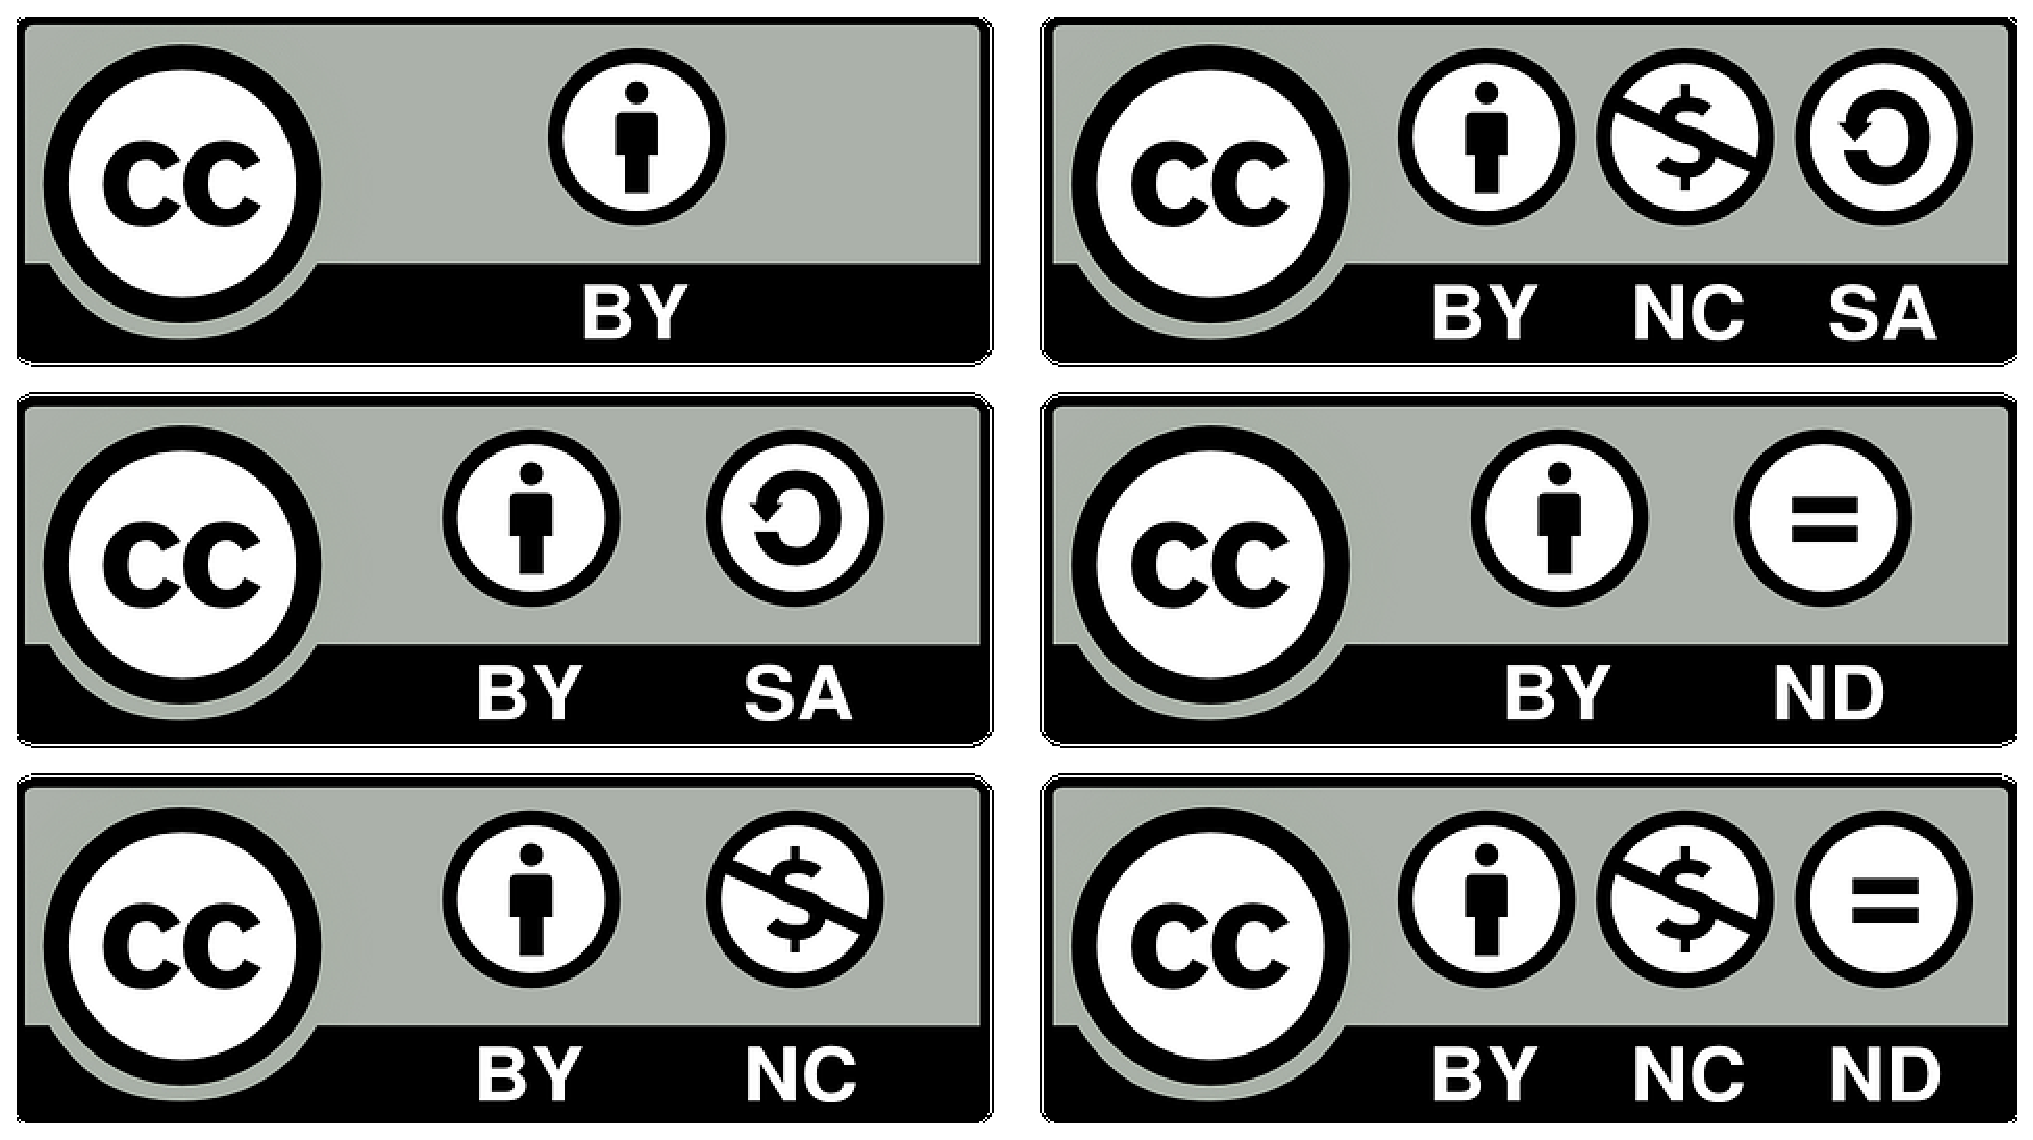
\includegraphics[trim=0 180 490 180,clip,width=20mm]{img/cclicense.eps}}
  \end{minipage} & 
  \begin{minipage}[c]{50mm}\footnotesize
   Hilofumi Yamamoto, Ph.D. \rule[-.0pt]{0pt}{8pt} \\
   Institute of Science Tokyo 
  \end{minipage}\\
 \end{tabular}


\ifEnglish
\setlength{\parindent}{3em}
\else
\fi

\ifPREFACE
\ifEnglish
\chapter*{Preface}
\else
\chapter*{はじめに}
\fi

\ifEnglish
This is a textbook that I wrote initially for the courses held at Institute of Science Tokyo {\itshape Strategic Japanese\/}.
\else
本書は著者が東京科学大学で開講していた日本文化コース、ストラテジック・ジャパニーズの教科書「ストラテジック・ジャパニーズ」のうち、「自然な話し方」を抜き出した分冊である。
\fi
\ifEnglish
Perhaps two natural approaches are needed to achieve {\it Natural speaking\/}:
one is that the conversation itself is natural; and the other is that the way of learning is natural.
\else
おそらく「自然な話し方」を達成するためには、2つの自然なアプローチが必要であろう。
1つは、会話自体が自然であること、もう1つは学び方が自然であることである。
\fi
\ifEnglish
This book, ``Japanese: Natural Steps; How to Speak Naturally,'' does not explain the rules of sentence structure and word order in detail.
\else
「自然な話し方」は文型、語順というルールをあえて無視すること。
\fi
\ifEnglish
On the other hand, ignoring the word order in a phrase or using verbs without conjugating them correctly can make a big difference in the meaning and not convey what you want to say, so these are explained in detail and stressed to be practiced.
\else
一方、句の中の語順を無視すること、動詞を正確に活用しないで使うことは、意味が大きく違ってしまい、言いたいことが伝達できないので、これらについては詳しく説明し、練習するように強調している。
\fi
\ifEnglish
If you keep this in mind, you can speak Japanese relatively freely.
\else
このことを押さえておけば、日本語は比較的自由に話せる。
\fi

\ifEnglish
Skills are developed gradually by working a little harder and improving a little more, but when I look at a beginner's textbook, it contains long sentences that students cannot seem to remember.
\else
技術は少しずつ難しくしてだんだん上手になっていくものなのに、初級の教科書を見ると、とうてい覚えられそうもないような長い文が出てくる。
\fi
\ifEnglish
We cannot remember it, so we cannot say it.
\else
覚えられないのだから、言えるはずもない。
\fi
\ifEnglish
Difficulty in conversation and pronunciation is a problem not on the learning side, but on the teaching side.
\else
会話が難しいとか発音が難しいとかは、学ぶ側の問題ではなく、教える側の問題だ。
\fi
\ifEnglish
It makes students uneasy and deprives them of their self-confidence because teachers have not analyzed the reality of what it means for students to really open their mouths.
\else
教師が本当に口を開くとはどういうことなのか、その現実を分析していないから、学生に不安を与え、学生の自信を奪う。
\fi
\ifEnglish
The lack of analysis of conversational scenes by teachers can also be inferred from the fact that teachers treat students in the early stages of language learners as if they were children.
\else
教師の会話場面の分析不足は、教師が言語学習初期の学生を子供のように扱うことからも推測できる。
\fi
\ifEnglish
Short utterances are not childish.
\else
短い発話は、子供っぽい言い方ではない。
\fi
\ifEnglish
Childishness is in the content to be dealt with.
\else
子供っぽさは扱う内容にある。
\fi
\ifEnglish
There are many short forms of communication in the contents done by adults.
\else
大人の文脈で短く表現されるコミュニケーションはいくらでもある。
\fi
\ifEnglish
It is the teacher's responsibility to extract that from the reality and show students the scenes that are needed for them.
\else
その現実を取り出し、必要とされる場面を見せることが教師の仕事だと考えている。
\fi

\vspace*{1\baselineskip}

% 00万とか1000万とか、そういう世界。

\begin{flushright}
\ifEnglish
Hilofumi Yamamoto, Ph.D.\\
Professor of Linguistics\\
Institute of Science Tokyo 
\else
{\large 山 元 啓 史}\hspace*{3zw}\\
{\small 東京科学大学教授}\hspace*{2zw}\\
\fi
\end{flushright}
\fi%PREFACE

\ifVOICE
\input{ling-a-voice.tex}
\fi%VOICE

\ifSHORTNOTES
\input{ling-a-notes.tex}
\fi%SHORTNOTES

\tableofcontents
%\listoffigures
%\listoftables
%\lstlistoflistings

\mainmatter


\ifOUTLINEOFLANGUAGESTRUCTURE
\ifEnglish
\chapter{Outline of Language Structure}
\else
\chapter{言語構造の概要}
\fi

\begin{abstract}
\ifEnglish
There isn't much you need to know before starting conversation practice.
\else
会話練習を始める前に知っておくべきことはあまりない。
\fi
\ifEnglish
Students should focus on practicing real conversation and writing.
\else
学生は実際の会話や作文の練習に集中すればよい。
\fi
\ifEnglish
However, it is advisable to learn beforehand how to sustain actual practice and understand the minimum structure of the language.
\else
ただし、あらかじめ、実際の練習を長続きさせるための工夫や、最低限の言語の仕組みを学んでおいたほうが良い。
\fi
\end{abstract}

\ifEnglish
\section{Structure and Discourse}
\else
\section{構造と会話の流れ}
\fi

\ifEnglish
Pay attention to the structure of the Japanese language and the flow of conversation.
\else
日本語という言語の構造と会話の流れに注目すること。
\fi
\ifEnglish
The word order of Japanese is relatively free.
\else
日本語の語順は、比較的自由である。
\fi
\ifEnglish
Subjects can be omitted as long as they are clear from the context.
\else
主語は文脈で理解できる限り、省略しても良い。
\fi
\ifEnglish
This is not limited to Japanese.
\else
これは日本語に限られたことではない。
\fi
\ifEnglish
In any language, word order is often flexible, and especially in conversation, many words can be omitted as long as the speaker and actions are clear to both parties.
\else
どの言語でも、語順はかなり自由であり、特に会話において、話者や動作主がわかれば、多くの語が省略できる。
\fi
\ifEnglish
Therefore, you can speak in whatever order feels most natural to you.
\else
したがって、思った順に安心して話してもよい。
\fi
\ifEnglish
This does not mean you are free to change the order of all words or omit any word as you please.
\else
ただ、まったく自由にすべての語の順序を変えたり、好きな語を省略してもよい、というわけではない。
\fi

\begin{toiquestion}
\ifEnglish
When speaking your mother tongue, think about whether you can omit the subject.
Consider if it is acceptable to omit it in conversation, and if it is appropriate to omit it in written language.
\else
自分の母語を話す時、主語を省略してもよいかどうかを考えなさい。
会話の中で省略してもよいか、また、書きことばでも省略してよいかどうかを考えなさい。
\fi
\end{toiquestion}

% 20241111
\begin{toianswer}
\ifEnglish
One-word utterances can be found in every language.
If only the most important words are spoken and the meaning is clear, one word can convey the message.
If the meaning is ambiguous, add words to clarify.
Whether it is a subject or an object depends on the context.
Whether it can be omitted also depends on the context, but in many cases, it should be omitted.
\else
どの言語でも、一語の発話が見られる。
最も大切な語だけを発話して、意味が明確であれば、一語で意味が伝わる。
もし意味が曖昧なら、語を追加して、曖昧さを解消する。
それが主語であるか、目的語であるかは、そのときの文脈による。
省略してもよいかどうかも文脈によるが、多くの場合、省略してよいはずだ。
\fi
\end{toianswer}

\ifEnglish
\subsection{Word order}
\else
\subsection{語順}
\fi

\ifEnglish
The word order of Japanese is relatively free.
\else
日本語の語順は比較的自由である。
\fi
\ifEnglish
However, the order in words and phrases cannot be changed.
\else
ただし、語や句の中の順番は変えられない。
\fi
\ifEnglish
The order in which the verbs are taught in the textbook is correct.
\else
動詞の形は教科書で教える順が正しい。
\fi
\ifEnglish
The verb is followed by an auxiliary verb that represents tense or voice.
\else
動詞の後に時制や態を表す助動詞が来る。
\fi
\ifEnglish
The order is never reversed.
\else
その順番が逆になることは決してない。
\fi
\ifEnglish
If the order,  (noun 2) of (noun 1), changes into the order, (noun1) of (noun 2), the meaning with the both will be completely different.
\else
(名詞1)の(名詞2)が(名詞2)の名詞1)の形になったら意味はぜんぜん違ってしまう。
\fi
\ifEnglish
We cannot change the word order in the phrase.
\else
句の中の語順を変えてはいけない。
\fi
\ifEnglish
The word order in verb phrases and noun phrases cannot be changed either.
\else
動詞句や名詞句の中の語順は変えられない。
\fi
\ifEnglish
These should be thought of as relatively long verbs, long nouns, rather than a series of words.
\else
これらはいくつかの単語がつながったものと考えるのではなく、比較的長い形の動詞、長い形の名詞と考えるべきである。
\fi
\ifEnglish
With that in mind, the Japanese word order may be in the order in which the speaker thinks what he or she wants to say.
\else
そのように考えると、日本語の語順は話し手がいいたいことを考えた順番で話しても良いことになる。
\fi
\ifEnglish
You can speak words according to your thought order.
\else
思考の順序で話してよい。
\fi
\ifEnglish
That would be the least stressful way of speaking.
\else
それがもっとも脳に負担を掛けない話し方であろう。
\fi

\begin{toiquestion}
 \ifEnglish
 When speaking your mother tongue, consider whether you can speak the order of the words relatively freely.
 \else
 自分の母語を話す時、語の順番は比較的自由に話してもよいかどうかを考えなさい。
 \fi
\end{toiquestion}

\ifEnglish
\subsection{Omission of particles}
\else
\subsection{助詞の省略}
\fi

\ifEnglish
A particle is added after the noun.
\else
名詞の後には助詞をつける。
\fi
\ifEnglish
It is when writing letters and academi papers, and it is more natural to omit particles in conversation.
\else
それは手紙や論文を書く時で、会話では助詞を省略する方が自然である。
\fi
\ifEnglish
However, there are particles that cannot be omitted depending on the context.
\else
ただし、文脈によって省略できない助詞がある。
\fi
\ifEnglish
In the case of moving verbs, to go, to come, to depart, to arrive, and so on, the destination `ni', the operating place `de', the departure place `o', and so on are necessary to clarify the meaning.
\else
移動の動詞、行く・来る・出発する・到着するなどの場合、到着地「に」、動作場所「で」、出発地「を」などは意味をはっきりさせるために必要である。
\fi
\ifEnglish
If we feel that the word order is different from other languages, it is better to think that it is not different as the structure of the language, but that the word order is used because of the structure of society and culture.
\else
語順が他の言語と違うと感じられるのであれば、それは言語の構造として違うのではなく、社会や文化の構造が原因でその語順が使われていると考えたほうが良い。
\fi
\ifEnglish
It may be a roundabout way of saying, but it may be advantageous to acquire cultural knowledge before learning a language.
\else
遠回りのように感じるかもしれないが、言語よりもむしろ先に文化の知識を身につけておく方が言語の習得に有利であろう。
\fi


\begin{toiquestion}
\ifEnglish
Discuss whether your mother tongue has equivalents to Japanese particles.
Also discuss the differences between it and Japanese particles.
\else
あなたの言語に日本語の助詞に相当するものがあるかどうか考えよ。
また、それと日本語の助詞との相違についても話し合え。
\fi
\end{toiquestion}


\ifEnglish
\subsection{Conjugations of verbs}
\else
\subsection{動詞の活用}
\fi
\ifEnglish
Do not make a mistake on the conjugations of verbs.
Misusing verb conjugations is the same as using different words.
\else
動詞の活用は間違えてはいけない。
動詞の活用を間違えるのは、違う単語を使っているのと同じである。
\fi
\ifEnglish
Note the sound of the predicate centered on the verb.
\else
動詞を中心とする述部の音には注意せよ。
\fi
\ifEnglish
In the predicate, various small sounds are connected to form one meaningful element (character string).
\else
述部にはさまざまな小さな音が連なって意味ある文字列になっている。
\fi
\ifEnglish
Among them, the sounds related to the conjugation of verbs play an important role.
\else
その中でも動詞の活用に関わる音は重要な意味を担う。
\fi
\ifEnglish
Therefore, it is necessary to practice so that the verb form that matches the meaning can be uttered promptly.
\else
ゆえに意味に即した動詞の形が速やかに発声できるような練習が必要である。
\fi

\begin{toiquestion}
\ifEnglish
The conjugations of verbs are complicated and various.
Consider whether each verb form is evenly used.
Also, consider which is the most commonly used form.
\else
動詞の活用形は複雑かもしれないが、それぞれの活用形が同じ頻度で使われているかどうかを考えなさい。
また、どれがもっともよく使われる形か考えなさい。
\fi
\end{toiquestion}

\ifEnglish
\section{Learning Strategy of Grammar}
\else
\section{文法の学び方}
\fi

\ifEnglish
Learn from commonly used verbs and commonly used forms. You don't need to learn all the conjugated forms since not all of them are used.
\else
よく使われる動詞、よく使われる形から学ぶこと。
すべての活用形が同じ頻度で使われるわけではないので、活用形のすべてを覚える必要はない。
\fi
\ifEnglish
Don't just learn words and expressions because they are frequent, but learn the order in which they are easy to remember and the techniques for remembering them.
\else
単に頻度が高いからという理由で学ぶのではなく、覚えやすい順番と覚え方の技術を身につけること。
\fi
\ifEnglish
Find a form that you can use immediately, and use it immediately before you forget it. Repeat this.
\else
すぐに使える形を見つけ、忘れる前にすぐ使う。
これを繰り返す。
\fi

\begin{toiquestion}
\ifEnglish
Check out the following words in Japanese: `go', `come', `eat', `is', and `do'.
Think and practice how to remember these five verbs right now.
\else
「行く」「来る」「食べる」「いる」「する」は日本語で何というかを調べなさい。
この5つの動詞を今すぐ覚える方法を考え、実践してみなさい。
\fi
\end{toiquestion}


\ifEnglish
\subsection{Utterance}
\else
\subsection{発話}
\fi

\ifEnglish
Utterance is the act of physically breathing out.
\else
発話は物理的に息を出す行為である。
\fi
\ifEnglish
Think of a way to speak with as little energy as possible.
\else
できるだけエネルギーを使わないで発話する方法を考えること。
\fi
\ifEnglish
The simplest response is to convey your intentions with only facial expressions and nods, without speaking.
\else
もっとも簡単な返答は、発話せず、表情やうなずきだけで意思を伝えることである。
\fi
\ifEnglish
There is a limit to ``do not speak,'' so when speaking, remember short phrases of about 3 words and speak them promptly.
\else
「発話しない」には限度があるので、発話する場合は、3語程度の短い句を覚え、その短い句を速やかに発話する。
\fi
\ifEnglish
If it's a short phrase, you can remember it without knowing the spelling.
\else
短い句であれば、綴を知らなくても覚えられる。
\fi
\ifEnglish
I think that 3 words is the limit to say in a breath in conversation.
\else
会話で一息で言うには3語が限度と考える。
\fi
\ifEnglish
Let's try to make a game that speaks quickly in 3 words as a group activity.
\else
3語で素早く発話するゲームをグループ活動で作ってやってみる。
\fi

\begin{toiquestion}
\ifEnglish
Think of a simple phrase that can be said in about three words.
\else
3語程度で言える簡単なフレーズを考えなさい。
\fi
\end{toiquestion}


\ifEnglish
\subsection{Verbs}
\else
\subsection{動詞}
\fi

\ifEnglish
Verbs are one of the most important sentence element in constructing a sentence.
Verbs have conjugations.
Each verb has a basic meaning, and at the same time, each conjugation has a meaning.
For beginners, it is recommended to remember the dictionary form and the negative form in pairs.
\else
動詞は、文を構成する上でもっとも重要な文の要素である。
動詞には活用がある。
それぞれの動詞には基本的な意味があると同時に、活用形毎に意味がある。
初心者には、辞書形と否定形を対で覚えることをお勧めする。
\fi
\ifEnglish
That way, you will not have a hard time making a {\it te form\/}.
\else
そうすれば「テ形」を作るのに苦労しない。
\fi
\ifEnglish
Learn dictionary form, negative form, and te form, just like you can learn multiplication tables and lyrics of popular songs.
\else
掛け算の九九や歌謡曲の歌詞を覚えるように、辞書形、否定形、テ形を覚える。
\fi
\ifEnglish
It is not realistic to think about conjugations and speak in the middle of a conversation.
\else
会話の途中で活用形を考え、発話するのは現実的ではない。
\fi
\ifEnglish
There is no point in unrealistic practice.
\else
現実的でない練習に意味はない。
\fi
\ifEnglish
In conversation, focus on the te form of the verb.
\else
会話では、動詞のテ形を中心に話すこと。
\fi
\ifEnglish
If you use the te form, you can express anything of past phrases, future phrases, present phrases, orders, requests, and impressions.
\else
テ形を使えば、過去でも未来でも現在の状態でも命令でも依頼でも感想でも何でも表現できる。
\fi
\ifEnglish
``I looked at it, and the I thought, was it blue?'' ``Yesterday, I did it'' ``Tomorrow, I will go to college'' ``Please eat it ...,'' and so on.
\else
「それ見て、思って、青かな?と」「昨日、やって」「明日、行って、大学へ」「どうぞ、食べて…」など。
\fi

\ifEnglish
Memorize verbs in the order of Group III, II, and I verbs.
\else
動詞の活用は、IIIグループ、IIグループ、そしてIグループの順に覚えること。
\fi
\ifEnglish
Group III verbs are frequently used in daily life.
\else
IIIグループは日常生活で頻繁に使われる。
\fi
\ifEnglish
The stem of Group II verbs does not change.
\else
IIグループは語幹が変化しない。
\fi
\ifEnglish
If you remember first that the negative stem of Group I verbs is `A' dan, the others are Group II or III verbs.
\else
Iグループは否定形の語幹がア段であることを先に覚えておけば、それ以外はIIあるいはIIIグループである。
\fi
\ifEnglish
In summary, the following three points are sufficient for memorizing the conjugations of verbs:
\else
まとめると、動詞の覚え方は、次の3点で十分である。
\fi

\begin{enumerate}
\ifEnglish
  \item A verb should be memorized by pairing a dictionary form and a negative form,
  \item Remember Group III, II, and I verbs in that order, and
  \item If {\it a\/} is in front of {\it nai\/}, it is a verb belongs to Group I, and if {\it i\/} or {\it e\/} should be considered as they belong to Group II.
\else
  \item 動詞の活用形は、辞書形と否定形の対で練習
  \item IIIグループ、IIグループ、そしてIグループの順に練習
  \item 「ない」の前が{\it a\/}ならIグループ、{\it i\/}あるいは{\it e\/}ならIIグループ
\fi
\end{enumerate}

\begin{toiquestion}
\ifEnglish
Check out the following words in Japanese: `go', `come', `eat', `is', and `do'.
Think and practice how to remember these five verbs right now.
\else
「行く」「来る」「食べる」「いる」「する」は日本語で何というかを調べなさい。
この5つの動詞を今すぐ覚える方法を考え、実践してみなさい。
\fi
\end{toiquestion}

\ifEnglish
\subsection{Adjectives: i-Adjective and na-Adjective}
\else
\subsection{形容詞: イ形容詞、ナ形容詞}
\fi

\ifEnglish
As with verbs, adjectives (i-adjectives) should be practiced in pairs with dictionary and negative forms.
\else
形容詞(イ形容詞)も動詞と同様、辞書形と否定形をペアで練習するとよい。
\fi
\ifEnglish
``ii? yokunai?''(Good or not good?) ``sugoi? sugokunai?''(Awesome or not?)  ``oishii? oishikunai?''(Delicious or not?) and so on.
\else
「いい?よくない?」「すごい?すごくない?」「おいしい?おいしくない?」など。
\fi
\ifEnglish
This is not a strange usage.
\else
これは別に変な使い方ではない。
\fi
\ifEnglish
Rather than that, it has the ability to seek emphasis, consent, and empathy, a pattern often found in actual Japanese conversation.
\else
むしろ、これには強調、同意、共感を求める機能があり、実際の日本語会話に頻繁に見られるパターンである。
\fi
\ifEnglish
It is convenient to remember na-adjectives as a pair of dictionary and negation.
Na-adjective should be remembered with a noun phrase, ``beautiful flower'' with a noun at the end.
It is also practical to add a noun to the end and remember it as a noun phrase such as {\it kireina hana\/} (beautiful flower).
{\it genkina hito\/} (energetic people), {\it yuumeina tokoro\/} (famous places) {\it taihenna keiken\/} (great experiences), etc.
\else
ナ形容詞も、辞書形、否定形のペアで覚えておくと便利である。
後ろに名詞をつけて「きれいな花」と名詞句で覚えるのも実用的である。
「元気な人」「有名なところ」「たいへんな経験」など。
\fi

\begin{toiquestion}
\ifEnglish
There are two types of Japanese adjectives. Describe the characteristics of each.
\else
日本語の形容詞は2種類ある。それぞれの特徴を述べよ。
\fi
\end{toiquestion}


\ifEnglish
\subsection{Proper noun first}
\else
\subsection{固有名詞が先}
\fi

\ifEnglish
Learning language is learning the culture where the language is spoken.
\else
言語を学ぶということは、文化を学ぶということである。
\fi
\ifEnglish
Learning culture is learning the language with that the culture is expressed.
\else
文化を学ぶということは、言語を学ぶということである。
\fi
\ifEnglish
Language that has been separated from the culture does not exist.
\else
文化と切り離された言語は存在しない。
\fi
\ifEnglish
The word `s\=up\=am\=aketto'  itself may exist, but the proper noun `Toky\=u suto\=a (Tokyu store)' is used more than the word itself.
\else
スーパーマーケットということばそのものは存在するが、実際にはそれよりも、「東急ストア?」「東急、行く?」のように固有名詞が使われる。
\fi
\ifEnglish
Rather than the word, `hanb\=ag\=ashoppu (hamburger shop), ``Makudonarudo (the McDonald's) is more familiar than that and people often shortly use the word `makudo'.
\else
ハンバーガーショップということばよりも、「マクドナルド」「マック」「マクド」が実際には使われる。
\fi
\ifEnglish
To learn proper nouns than general nouns is practical in that they directly depend on the culture.
\else
一般的な名詞を学ぶよりも固有名詞、すなわち文化(上記の例であれば特定地域)に直接依存した語の方が現実的である。
\fi

\begin{toiquestion}
\ifEnglish
When speaking in your own language, think about which is more commonly used, proper nouns or general nouns, for things that are closely related to your life, such as supermarkets and convenience stores.
\else
自分の言語で話す時、スーパーマーケットやコンビニエンスストアなど、生活に密接なものは、固有名詞と一般名詞とどちらがよく使われているかを考えなさい。
\fi
\end{toiquestion}

\ifEnglish
\subsection{Slang and Idiom}
\else
\subsection{俗語と慣用句}
\fi

\ifEnglish
Slang and idioms are also important.
\else
俗語と慣用句も重要である。
\fi
\ifEnglish
Slang is a limited-time word born from an era-dependent situation.
\else
俗語はその時代に依存した状況から生まれてきた、期間限定の語である。
\fi
\ifEnglish
Buzzwords and youth words have similar qualities.
\else
流行語も若者ことばも類似の性質を持っている。
\fi
\ifEnglish
For example, {\it man-neri\/} (in a rut), {\it maji?\/} (seriously?), {\it ch\=o-muzu\/} (super-difficult), {\it bochi-bochi\/} (little by little), {\it yan'nacchau\/} (no way!), {\it akimahen\/} (cannot do it),{\it s\-oiu mon'yo\/} (That's what it is), {\it dasai\/} (tackey, lame), {\it yabai\/} (crapy), and so on.
\else
たとえば、マンネリ (in a rut)、 マジ?、 超ムズ、 ぼちぼち、 やんなっちゃう、 あきまへん、 そういうもんよ、 ダサい、 やばい、 などのことばである。
\fi

\begin{toiquestion}
\ifEnglish
Think about whether youth language and slang are used in your language.
\else
自分の言語で、若者ことばと俗語が使われているかどうか、考えてみなさい。
\fi
\end{toiquestion}

\ifEnglish
\subsection{The shortest form, also quick response}
\else
\subsection{短い言い方と素早い返答}
\fi

\ifEnglish
Life of the conversation is speed.
\else
会話の命はスピードである。
\fi
\ifEnglish
As long as it is the representation from the mouth, speed is the most important.
\else
表現を口から出す限り、スピードは最も大切である。
\fi
\ifEnglish
To ensure speed, language form must be shortest and a speaker must react immediately.
\else
スピードを確保するには、言語の形式はもっとも短く、即座に反応することである。
\fi
\ifEnglish
The shortest form should be learned in advance, and it is necessary to train mouth and throat muscles to speak them.
\else
もっとも短い形式をあらかじめ学び、それを発話する口や喉の筋肉を鍛える必要がある。
\fi
\ifEnglish
Do not keep silent when asked by the person you're talking to.
\else
話し相手から聞かれたら、黙っていてはいけない。
\fi
\ifEnglish
Get used to the rhythm of responding instantly in a short form.
And prepare a lot of short, easy-to-pronounce phrases.
The short form is the most economical and easy-to-pronounce linguistic form that is easy to convey to the person you are talking to.
\else
短い形で即座に返答するリズムに慣れること。
そして短い発音しやすいフレーズをたくさん準備しておくこと。
短い形は、もっとも経済的で発音しやすい形で相手に伝わりやすい言語形式である。
\fi
\ifEnglish
React immediately.
If you cannot do that, say something like {\it e-tto-\/}, {\it ano-\/}, and just react immediately.
\else
即座に反応すること。
それができない場合には、「ああ、えーと」などを使い、反応だけでも即座に行う。
\fi

\begin{toiquestion}
\ifEnglish
Even in your own language, if you cannot respond immediately, you are probably uttering something and reacting.
Think about what words you are using to respond.
\else
自分の言語でも、すぐに返答できないとき、何か発話して反応しているだろう。
どんなことばで反応しているか、を考えてみなさい。
\fi
\end{toiquestion}
%最適化された、経済的な形は短い形。
%最小努力の法則。


\ifEnglish
\subsection{Politeness}
\else
\subsection{丁寧さ}
\fi

\ifEnglish
It is important to note that formal speech should not be mixed with casual speech.
\else
フォーマルな言い方をする時には、カジュアルな言い方を混ぜてはいけないことに気をつけなければならない。
\fi
\ifEnglish
Many students say that honorifics are difficult.
\else
多くの学生は敬語が難しいという。
\fi
\ifEnglish
Remembering honorifics is not difficult at all.
\else
敬語を覚えることは決して難しくない。
\fi
\ifEnglish
It's not too difficult to judge the relationship between yourself and the listener.
\else
自身と聞き手との関係を判断するのもそんなに難しくはない。
\fi
\ifEnglish
So what's difficult?
\else
では、何が難しいのか。
\fi
\ifEnglish
There is a rule that casual and formal expressions should not be mixed in the same sentence.
\else
カジュアルな表現とフォーマルな表現を同じ文に混ぜて使ってはいけないというルールがある。
\fi
\ifEnglish
It is difficult to pay attention not to mix casual expressions with honorific sentences.
\else
敬語の文にカジュアルな表現が混ざらないように注意するのは難しい。
\fi
\ifEnglish
For example,  {\itshape dakedo\/}(but), {\itshape keredo\/}(even though; but), are good words for casual conversation.
They, however, should never be mixed in formal conversation.
In formal style, {\itshape desukedo\/}(but), {\itshape desukeredomo\/}(but), or {\itshape shikashi\/} should be used.
\else
たとえば、「だけど」「けれど」はカジュアルではよいことばではあるが、フォーマルに絶対混ぜられないことばである。
フォーマルスタイルでは、「ですけど」もしくは「ですけれども」、「しかし」を用いなければならない。
\fi

\begin{toiquestion}
\ifEnglish
Think about whether you can mix casual and formal styles in your own language.
\else
自分の言語でも、カジュアルとフォーマルのスタイルを混ぜて使ってもよいかどうかを考えなさい。
\fi
\end{toiquestion}

\ifEnglish
\section{Recommendations}
\else
\section{推薦するもの}
\fi

\ifEnglish
There are various books (Japanese textbooks, dictionaries, manga, magazines), CDs, the Internet, mobile phone apps, etc.
Besides, if you include food packages, signs on the streets, menus, etc., you will always have resources to learn Japanese by your side.
\else
書籍(日本語教科書、辞書、マンガ、雑誌)、CD、インターネット、携帯電話アプリ等、さまざまなものがある。
他にも、食品のパッケージ、看板、掲示、メニュー、等を入れれば、日本語を学ぶためのリソースはいつでもそばにある。
\fi

\ifEnglish
\subsection{References}
\else
\subsection{参考書}
\fi

\ifEnglish
If you do not feel the need to rely on a grammar book, you do not need to use any.
A reference book which includes many examples sentences is recomended since the grammar description alone will not explain you how to use it.
\cite{Kaiser_Butler200103} is one of the choices we recommend as a dictionary which includes significant examples.
\else
文法書に頼る必要性を感じなければ、何も使わなくてもよい。
文法だけを見ても使い方はわからないので、例文が多く書かれている参考書が良い。
\cite{Kaiser_Butler200103}は実際の新聞記事より採取した例文が掲載されている数少ない選択肢の1つである。
\fi

\ifEnglish
\subsection{Internet resources}
\else
\subsection{インターネットのリソース}
\fi

\ifEnglish
Fan sites with subtitled songs, dramas, and drama scenarios, all of which can be used for shadowing.
Subtitles are useful for training in short reading comprehension.
\else
字幕付きの歌、ドラマ、ドラマシナリオが掲載されているファンサイト、これらはすべてシャドウイングに使える。
字幕は、短文読解の訓練に役立つ。
\fi

\ifEnglish
\subsection{Dictation for Every Day (D4E)}
\else
\subsection{ディクテーション: D4E}
\fi

\ifEnglish
The practice of listening to the same sentence over and over is necessary to confirm your language recognition.
\else
同じ文を何回も聞く練習は、自分の言語認識を確認するのに必要である。
\fi
\ifEnglish
Dictation is convenient for that training.
\else
ディクテーションはその訓練に便利である。
\fi
\ifEnglish
However, it is difficult for language learners to judge whether what they wrote was correct.
\else
しかし、自分の書いたものが正しかったかどうか、自分で判断するのは難しい。
\fi
\ifEnglish
It would be convenient to have an on-site application where the computer system displays the scoring results.
\else
採点結果をコンピュータシステムが表示するオンサイトアプリケーションがあれば、それは便利である。
\fi
\ifEnglish
The audio obtained from the system is useful not only for writing down, but also for aloud shadowing.
\else
そのシステムから得られる音声は、書き取るだけでなく、声に出してシャドウイングを行うのにも便利である。
\fi

\begin{toiquestion}
\ifEnglish
Try practicing with D4E(Dictation for Every day)\footnote{D4E: \href{https://cuckoo.js.ila.titech.ac.jp/~yamagen/d4ev5/index?proj=d4e}{\url{https://cuckoo.js.ila.titech.ac.jp/~yamagen/d4ev5/index?proj=d4e}}}, and exchange ideas about what you noticed during the practice.
\else
D4E\footnote{D4E: \href{https://cuckoo.js.ila.titech.ac.jp/~yamagen/d4ev5/index?proj=d4e}{\url{https://cuckoo.js.ila.titech.ac.jp/~yamagen/d4ev5/index?proj=d4e}}}
を使って実際にディクテーションの練習をしてみなさい。
そして練習中に気がついたことについて意見交換をしなさい。
\fi
\end{toiquestion}
\fi%OUTLINEOFLANGUAGESTRUCTURE

%%%%%%%%%%%%%%%%%%%%%%%%%%%%%%%%%%%%%%%%%%%%%%%%%%%%%%%%
%%%%%%%%%%%%%%%%%%%%%%%%%%%%%%%%%%%%%%%%%%%%%%%%%%%%%%%%
%%%%%%%%%%%%%%%%%%%%%%%%%%%%%%%%%%%%%%%%%%%%%%%%%%%%%%%%
%%%%%%%%%%%%%%%%%%%%%%%%%%%%%%%%%%%%%%%%%%%%%%%%%%%%%%%%

\ifSTARTFROMTHEBASICS
\ifEnglish
\chapter{Start from the Basics}
\else
\chapter{まずは基礎から}
\fi%English

\begin{abstract}
\ifEnglish
You do not have to learn all the basics of Japanese first.
You may learn this first, but it is almost useless to remember grammar rules without actually using them.
It is, therefore, effective to look back on the basics during your conversation practices.
Regarding this chapter as a reference, return to this chapter while practicing the chapter called ``Natural Speaking'' in the followings.
\else
日本語の基礎ははじめに全部を学ぶ必要はない。
学んでもよいが、実際に使うこともせずして、覚えることは無駄に近いので、使いながら、基礎に振りかえってみるのが効果的である。
この章はレファレンスぐらいに考えて、次の章の「自然な話し方」を実践しながら、この章に戻って確認するとよい。
\fi
\end{abstract}


\ifEnglish
\section{Quick reaction: Uchi kuru? (Wanna come my house?)}
\else
\section{すぐに反応する: うち、来る?}
\fi

%ファイル名: T51Preparation01.pdf: Uchi kuru? Quick reaction
\ifEnglish
The first thing to do is to practice the quick reaction.
It is important to practice the quick reaction to the Japanese language.
\else
まずは、すぐに反応する練習をする。
日本語の発話に慣れることが重要。
\fi
\ifEnglish
Activities include listening to three basic sentences, determining which one of the three it is, and answering it by number.
\else
基本文、3つを聞いて、3つのうちのいずれかであるかを判断し、それを番号で答える活動をする。
\fi

\ifEnglish
\subsection{Conversation patterns}
\else
\subsection{会話パターン}
\fi

\ifEnglish
The following patterns are often used in daily life in Japan.
\else
以下のパターンは日本の日常生活でよく使われる。
\fi

\ifEnglish
Q..Question sentence; A..Affirmative sentence; N..Negative sentence
\else
Q..疑問文; A..肯定文; N..否定文
\fi

\begin{figure}[htbp]
  \begin{center}
    \fbox{
\includegraphics[trim=80 90 70 60, clip, width=0.16\textwidth]
    {img/quickReactionQuestion01.png} }
    \hspace{0.1\textwidth}
    \fbox{
\includegraphics[trim=80 90 70 60, clip, width=0.16\textwidth]
    {img/quickReactionAffirmative01.png} }
    \hspace{0.1\textwidth}
    \fbox{
\includegraphics[trim=80 90 70 60, clip, width=0.16\textwidth]
    {img/quickReactionNegative01.png} }
  \end{center}
\ifEnglish
\caption{Three ways of quick reaction}
\else
\caption{3つのすぐに反応する方法}
\fi
  \label{fig:QuickReaction}
\end{figure}

\begin{enumerate}
\item 
\begin{itemize}
  \item [Q:] Uchi, kuru? (Do you come to my house?)
  \item [A:] Un, iku. (Yes, I will go.)
  \item [N:] Uun, ikanai. (No, I will not go.)
\end{itemize}
\item 
\begin{itemize}
  \item [Q:] Ge-mu, suru? (Do you play a game?)
  \item [A:] Un, suru. (Yes, I will do.)
  \item [N:] Uun, shinai. (No, I won't do.)
\end{itemize}
\item
\begin{itemize}
  \item [Q:] Kore, taberu? (Do you eat this?)
  \item [A:] Un, taberu. (Yes, I will eat it.)
  \item [N:] Un, tabenai. (No, I will not eat it.)
\end{itemize}
\item  
\begin{itemize}
  \item [Q:] Kore, miru? (Do you see it?)
  \item [A:] Un, miru. (Yes, I will see it.)
  \item [N:] Uun, minai. (No, I will not see it.)
\end{itemize}
\item 
\begin{itemize}
  \item [Q:] Ko-hi-, nomu? (Do you drink a coffee?)
  \item [A:] Un, nomu. (Yes, I will drink.)
  \item [N:] Uun, nomanai. (No, I will not drink.)
\end{itemize}
\end{enumerate}

\ifEnglish
\subsection{Tasks}
\else
\subsection{課題}
\fi

\begin{enumerate}
\ifEnglish
  \item React quiclky to your instructor's utterances using finger signs.
\else
  \item 指のサインを使って、インストラクターの発話にすぐに反応しなさい。
\fi
\ifEnglish
  \item Practice the five patterns above with your partner.
\else
  \item 上記の5つのパターンをパートナーと練習しなさい。
\fi
\ifEnglish
  \item Make a new conversation using the patterns with your partners.
\else
  \item パートナーと、新しい会話を作りなさい。
\fi
\end{enumerate}

\ifEnglish
\subsection{Discussion}
\else
\subsection{ディスカッション}
\fi

\begin{enumerate}
\ifEnglish
 \item How would you feel if you gave a short and quick answer?
\else
 \item 短かくすぐに答えるとどんな感じがするか。
\fi
\ifEnglish
 \item Look at the english and guess what each Japanese word means.
\else
 \item 英語を見て、日本語のそれぞれの単語はどんな意味かを推測しなさい。
\fi
\ifEnglish
 \item Think about how to make a question sentence in Japanese.
\else
 \item 日本語の疑問文はどう作るかを考えなさい。
\fi
\ifEnglish
 \item Find out what sound always appears at the end of the verb in negative sentences.
\else
 \item 否定文のとき、動詞の末尾にどんな音がいつもあるか、見つけなさい。
\fi
\ifEnglish
 \item Add words to these patterns and have a conversation using the new sentences.
\else
 \item これらのパターンに単語を加えて、新しい文を使って会話をしてみなさい。
\fi
\end{enumerate}

\subsection{Game}

\ifEnglish
In groups of three, each person asks a question to the person next to them.
The person asked the question must respond immediately.
The group that lasts the longest wins.
\else 
3人1組になって、1人ずつ、隣の人に質問をします。
質問された人は、すぐに返答しなければなりません。
1番長く続けたグループが勝ちです。
\fi

\ifEnglish
\section{Verb the Basics: A Day in My Life}
\else
\section{動詞の基本: 私のある1日}
\fi

%ファイル名: T51BasicVerb01V02.pdf: A day in my life.

\ifEnglish
It is very important as an introduction to Japanese, but unfortunately, this teaching material does not end in 60 minutes if you do it carefully.
\else
日本語の導入としてとても重要であるが、残念なことに、この教材は、じっくりやると60分では終わらない。
\fi
\ifEnglish
It suffices if you can roughly understand the whole picture of the verb sentence, which is the predicate that is important in utterance.
\else
発話で重要となる述部を担う、動詞文の全体像が大雑把に理解できればそれでよい。
\fi
\ifEnglish
It is an impactful teaching material to give an overview of the language of Japanese and to show that this language is systematic.
\else
日本語という言語の概要を示し、この言語がシステマティックであるということを示すにはインパクトがある教材である。
\fi

\ifEnglish
\subsection{Top 12 useful verbs}
\else
\subsection{最初の12の役立つ動詞}
\fi

\begin{table}[htpb]\small\centering
  \ifEnglish
  \caption{Top 12 useful verbs for the daily conversation}
  \else
  \caption{日常会話に役立つ動詞トップ12}
  \fi
  \label{tab:label}
  \begin{tabular}{lll}\noalign{\hrule height .8pt}
   1. suru (do III) &
   2. kuru (come III)&
   3. taberu (eat II.e)\\
   4. miru (see II.i)&
   5. kiku (drink I.k)&
   6. yomu (read I.m)\\
   7. nomu (drink I.m)&
   8. toru (take I.r)&
   9. kau (buy I.w)\\
   \hspace{-1ex}10. iku (go I.k*) &
   \hspace{-1ex}11. mottekuru (bring III)&
   \hspace{-1ex}12. kureru (give me II.e)\\
  \end{tabular}
\end{table}

\ifEnglish
Students will learn important 12 basic verbs and the outline of verbs through practicing verb conjugation:
\else
重要12動詞の活用練習を通して、動詞の基本あるいは概要を学ぶ。
\fi
\ifEnglish
Japanese verbs have conjugations, but not all conjugations are used at the same frequency.
\else
日本語の動詞には活用があるが、すべての活用は同じ頻度で使われるわけでない
\fi
\ifEnglish
Students do not have to be able to practice because the purpose is to see the whole picture of the verb.
\else
動詞の全体像を眺めることが目的なので、練習ができなくても良い。
\fi

\ifEnglish
There are three types of verbs in Japanese, called Group I, II, and III verbs, respectively.
\else
日本語の3種類の動詞があり、それぞれI, II, IIIグループと呼ばれている。
\fi
\ifEnglish
It is convenient to be aware of the grouping of verbs, but it will be a problem if students cannot distinguish between the I group verb {\it kiru\/} (to cut) and the I group verb {\it kiru\/} (to wear) whose the both of dictionary forms end with {\it ru\/}.
\else
動詞のグループ分けを意識すると便利であるが、辞書形が「る」で終わるIグループ動詞「切る」、IIグループ動詞「着る」の区別ができずに困るだろう。
\fi
\ifEnglish
Even if students remember it with its masu form, students cannot distinguish it if just the before `masu' is `i' such as {\it kaimasu\/} (to buy) or {\it imasu\/} (to be).
\else
ます形で覚えたとしても、「買います」「います」のように「ます」の前が「い」になっていたら区別はできない。
\fi
\ifEnglish
If students use it from the verbs that frequently appear, such as {\it kau $\rightarrow$ katte\/}, and {\it iru $\rightarrow$ ite\/} like learning multiplication tables, students will become not to make a mistake.
\else
掛け算の九九を学ぶように、「買う $\rightarrow$ 買って」「います $\rightarrow$ いて」と頻出する動詞から使っていれば、そのうち間違えないようになるだろう。
\fi
\ifEnglish
Students should not have to try too hard to remember.
\else
あまり覚えようと努力する必要もないはずだ。
\fi

\subsection*{Group III verbs: irregular verbs}

\ifEnglish
Learn from Group III verbs (irregular conjugation verbs) first.
\else
IIIグループ(不規則活用動詞)から先に学ぶ。
\fi


\begin{table}[htpb]\small\centering
  \ifEnglish
  \caption{Group III verbs;
   blue letters are stems;
   red letters are inflected flexions;
   the stem of Group III verbs does irregulary change.
  }
  \else
  \caption{IIIグループ動詞;
    青い文字は語幹;
    赤い文字は活用語尾;
    IIIグループ動詞の語幹は不規則に変化する。
  }
  \fi
  \label{tab:IIIgroupverb}
  \begin{tabular}{rrrrrrrr}\noalign{\hrule height .8pt}
      & negative & polite   & dictionary & conditional  & volitional& potential \\
      & -\textcolor{red}{nai}
      & -\textcolor{red}{masu}
      & -\textcolor{red}{ru}
      & -\textcolor{red}{reba}
      & -\textcolor{red}{you}
      & -\textcolor{red}{rareru}
      \\\hline
      \multicolumn{1}{l}{to do}
      & \textcolor{blue}{shi}\textcolor{red}{nai}
      & \textcolor{blue}{shi}\textcolor{red}{masu}
      & \textcolor{blue}{su}\textcolor{red}{ru}
      & \textcolor{blue}{su}\textcolor{red}{reba}
      & \textcolor{blue}{shi}\textcolor{red}{you}
      & dekiru
      \\
      \multicolumn{1}{l}{to come}
      & \textcolor{blue}{ko}\textcolor{red}{nai}
      & \textcolor{blue}{ki}\textcolor{red}{masu}
      & \textcolor{blue}{ku}\textcolor{red}{ru}
      & \textcolor{blue}{ku}\textcolor{red}{reba}
      & \textcolor{blue}{ko}\textcolor{red}{you}
      & \textcolor{blue}{ko}\textcolor{red}{rareru}
      \\
  \end{tabular}
\end{table}

\ifEnglish
There are only two verbs in the III group: {\it suru\/} (do) and {\it kuru\/} (come).
\else
IIIグループには、「する」「くる」の2種類の動詞しかない。
\fi
\ifEnglish
The conjugation of Group III verbs changes as shown in Table \ref{tab:IIIgroupverb}.
Since the stems of conjugations change in various ways, it is better to make sentences by yourself and actually use the sentences many times.
The stem of Group III verbs generally refers to the conjunctive form of the stem (the form of {\it kimasu\/} minus {\it masu\/}.
\else
活用は表\ref{tab:IIIgroupverb}のように変化する。
活用語幹が様々に変化するので、自分で文を作って、その文を実際に何度も使うのがよい。
IIIグループの語幹とは一般的に連用形の語幹(「来ます」から「ます」を取り除いた形)を言う。
\fi
\ifEnglish
Practice dictionary and negative forms in pairs, such as {\it suru\/} (do), {\it shinai\/} (do not), {\it kuru\/} (come), and {\it konai\/} (not come).
\else
「する」「しない」、「くる」「こない」のように辞書形・否定形をペアで練習する。
\fi
\ifEnglish
Make simple exchanges such as in Table \ref{tab:iiiGroupPractice}.
\begin{table}[htpb]\small\centering
  \caption{Simple practices of the III group verbs}
  \label{tab:iiiGroupPractice}
  \begin{tabular}{ll}\noalign{\hrule height .8pt}
                Japanese & English \\\hline
{\it okane aru? nai!\/} & Do you/we have money? No!\\
{\it jikan aru? nai!\/} & Do you/we have time? No!\\
{\it shukudai aru? nai!\/} & Do you/we have homework? No!\\
{\it benkyo suru? shinai!\/} & Do you study? No!\\
{\it ryouri suru? shinai!\/} & Do you cook? No!\\
{\it supo-tsu suru? shinai!\/} & Do you play sports? No!\\
{\it asu mo daigaku kuru? konai!\/} & Will you come to college tomorrow? No!\\
{\it asu mo kenkyuushitsu kuru? konai!\/} & Do you come to the labo tomorrow? No!\\
  \end{tabular}
\end{table}
\else
表\ref{tab:iiiGroupPractice}に示すような簡単なやりとりで練習をすると良い。
\begin{table}[htpb]\small\centering
  \caption{IIIグループ動詞の簡単な練習}
  \label{tab:iiiGroupPractice}
  \begin{tabular}{ll}\noalign{\hrule height .8pt}
                日本語 & 英語\\\hline
お金、ある? ない! & Do you/we have money? No!\\
時間、ある? ない! & Do you/we have time? No!\\
宿題、ある? ない! & Do you/we have homework? No!\\
勉強する? しない! & Do you study? No!\\
料理する? しない! & Do you cook? No!\\
スポーツする? しない! & Do you play sports? No!\\
明日も大学、くる? こない! & Will you come to college tomorrow? No!\\
明日も研究室、くる? こない! & Do you come to the labo tomorrow? No!\\
  \end{tabular}
\end{table}
\fi
\ifEnglish
If you talk like a game repeatedly, you can remember it naturally.
In this case, it is a dictionary form and a negative form learning method, but the same idea applies to the te form learning method.
\else
繰り返しゲームのように会話をすれば、自然に覚えられる。
この場合は辞書形と否定形の学び方であるが、テ型の学び方についても同じ考え方である。
\fi
\ifEnglish
The types of verbs should be increased over time.
It is more important to find and use various nouns that are used with verbs.
\else
動詞の種類は時間を掛けて増やしていけば良い。
それよりも動詞と一緒に使う名詞をいろいろ自分で探して使ってみることが重要である。
\fi
\ifEnglish
Look up a noun that suits your life in the dictionary and use it with the verb.
\else
自分の生活に即した名詞を辞書で探して、動詞といっしょに使うとよい。
\fi

\ifEnglish
We will practice {\it aru\/} (to have; there is) and {\it nai\/}(not have; there is no) as well.
\else
「ある」「ない」もここで練習する。
\fi
\ifEnglish
It may seem strange, but {\it aru\/} is a verb and {\it nai\/} is an i-adjective.
The difference in part of speech between {\it aru\/} and {\it nai\/} means that the language system is different.
\else
奇妙に思うかもしれないが、「ある」は動詞であり、「ない」はイ形容詞である。
「ある」と「ない」の品詞が違うということは、言語のシステムが違うということである。
\fi
\ifEnglish
Since the form of denial of {\it aru\/} is originally used as in the form of {\it aranu\/} or {\it arazu\/}, {\it aru\/} is conjugated as {\it arazu\/}, {\it arimasu\/}, {\it aru\/}, {\it areba\/}, {\it ar\=o\/}, so it is similar to I group conjugation.
\else
「ある」の否定の形は本来は「あらぬ」「あらず」なので、「あらず」「あります」「ある」「あれば」「あろう」と活用するので、五段活用に似ている。
\fi
\ifEnglish
However, in modern language, there is no usage of {\it arazu\/} and it is not common since it is used as a literary expression such as {\it aranu utagai wo kakerareta\/} (I am unsuspected) or {\it kare wa t\=ojin ni arazu\/} (he is not a thief).
\else
しかし、現代語では「あらない」という使い方はなく、文語的に「あらぬ疑いをかけられた」「彼は盗人にあらず」のように使われるので一般的ではない。
\fi
\ifEnglish
The negative form of {\it aru\/} uses an i-adjective {\it nai\/}.
\else
「ある」の否定形は形容詞の「ない」が使われる。
\fi
\ifEnglish
{\it Aru\/} is called {\it Ra-gyo henkaku katsuy\=o\/} (R-irregular conjugation) in Japanese linguistics.
\else
「ある」は日本語学ではラ行変格活用と呼ばれている。
\fi

\begin{toiquestion}
\ifEnglish
Follow Table \ref{tab:iiiGroupPractice} and practice conversation with your classmates.
After practice, check if you remember the dictionary and negative forms of Group III verbs
\else
表\ref{tab:iiiGroupPractice}に倣ってクラスメートと会話練習をしてみなさい。
練習後、IIIグループの動詞の辞書形と否定形が覚えられたかどうかを確認しなさい。
\fi
\end{toiquestion}


\subsection*{Group II: {\it i\/} subgroup and {\it e\/} subgroup}

\begin{table}[htpb]\small\centering
  \ifEnglish
  \caption{Group II verbs;
   blue letters are stems;
   red letters are inflected flexions;
   the stem of II group verb does not change.
  }
  \else
  \caption{IIグループ動詞;
    青い文字は語幹;
    赤い文字は活用語尾;
    IIグループ動詞の語幹は変化しない。
  }
  \fi
  \label{tab:IIgroupverb}
  \begin{tabular}{rrrrrrr}\noalign{\hrule height .8pt}
      &          &          &          &            & conditional &          \\
      &          & negative & polite   & dictionary & /potential  & volitional\\
      &
      & -\textcolor{red}{nai}
      & -\textcolor{red}{masu}
      & -\textcolor{red}{ru}
      & -\textcolor{red}{reba/reru}
      & -\textcolor{red}{you}
      \\\hline
      \multicolumn{1}{c}{\textcolor{blue}{i}}
      &\multicolumn{1}{l}{to wear}
      & k\textcolor{blue}{i}\textcolor{red}{nai}
      & k\textcolor{blue}{i}\textcolor{red}{masu}
      & k\textcolor{blue}{i}\textcolor{red}{ru}
      & k\textcolor{blue}{i}\textcolor{red}{reba/reru}
      & k\textcolor{blue}{i}\textcolor{red}{you}
      \\
      \multicolumn{1}{c}{\textcolor{blue}{e}}
      &\multicolumn{1}{l}{to eat}
      & tab\textcolor{blue}{e}\textcolor{red}{nai}
      & tab\textcolor{blue}{e}\textcolor{red}{masu}
      & tab\textcolor{blue}{e}\textcolor{red}{ru}
      & tab\textcolor{blue}{e}\textcolor{red}{reba/reru}
      & tab\textcolor{blue}{e}\textcolor{red}{you}
      \\
  \end{tabular}
\end{table}

\ifEnglish
There are two subclasses of Group II verbs: {\it Kami-ichidan d\=oshi\/}, the verb group of the second vowel {\it i\/} of {\it aiueo\/} with no inflection ending, and the verb group of the fourth vowel {\it e\/} with no inflection ending.
We will name the former Group II.i and the latter Group II.e in this book.
\else
IIグループ動詞には、下位分類として、母音のiが活用語尾である上一段動詞、と母音のeが活用語尾である下一段動詞の2種類がある。
本書では、前者をII.iグループ、後者をII.eグループと呼ぶことにする。
\fi
\ifEnglish
The same applies to Group II verbs. {\it gohan, taberu?\/} (do you eat rice?), {\it tabenai\/} (no, I don't), {\it terebi, miru\/} (do you watch TV?), {\it minai\/} (no, I don't), etc.
\else
IIグループも同様。「ごはん、食べる」「食べない」、「テレビ、見る」「見ない」など。
\fi
\ifEnglish
You can think of {\it miru\/} (see), {\it iru\/} (be), {\it kariru\/} (borrow), and {\it okiru\/} (get up) as verbs in II.i verbs.
\else
「見る」「いる」「借りる」「起きる」の4つがII.iグループの動詞としてよく使われると考えてよい。
\fi

\begin{toiquestion}
 \ifEnglish
 Write the conjugations of each of the following Group II verbs.
 \else
 つぎのIIグループの動詞についてそれぞれの活用形を書いてみなさい。
 \fi
\end{toiquestion}

   

\begin{table}[ht]\centering
\ifEnglish
 \caption{Conjugation table (II Group verbs)}
\else
 \caption{活用表 (IIグループの動詞)}
\fi
 \label{IIGroup}
% \vspace*{-.8\baselineskip}
\def\tabcolsep{2.0pt}
\def\arraystretch{.8}
\begin{tabular}{rrrrrrr}\noalign{\hrule height .8pt}
    &          &          &          &            & conditional &          \\
    &          & negative & polite   & dictionary & /potential  & volitional\\
    &
    & -\textcolor{red}{nai}
    & -\textcolor{red}{masu}
    & -\textcolor{red}{ru}
    & -\textcolor{red}{reba/reru}
    & -\textcolor{red}{you}
    \\\hline

    &\multicolumn{1}{l}{to wear}
    & k\textcolor{blue}{i}\textcolor{red}{nai}
    & k\textcolor{blue}{i}\textcolor{red}{masu}
    & k\textcolor{blue}{i}\textcolor{red}{ru}
    & k\textcolor{blue}{i}\textcolor{red}{reba/reru}
    & k\textcolor{blue}{i}\textcolor{red}{you}
    \\\hline

    1. &\multicolumn{1}{l}{to live}    & & &  ikiru       & & \\
    2. &\multicolumn{1}{l}{to be}      & & &    iru       & & \\
    3. &\multicolumn{1}{l}{to see}     & & &   miru       & & \\
    4. &\multicolumn{1}{l}{to wake up} & & &  okiru       & & \\
    5. &\multicolumn{1}{l}{to pass}    & & & sugiru       & & \\
    6. &\multicolumn{1}{l}{to fall}    & & & ochiru       & & \\
    7. &\multicolumn{1}{l}{to get off} & & &  oriru       & & \\
    \hline

    &\multicolumn{1}{l}{to eat}
    & tab\textcolor{blue}{e}\textcolor{red}{nai}
    & tab\textcolor{blue}{e}\textcolor{red}{masu}
    & tab\textcolor{blue}{e}\textcolor{red}{ru}
    & tab\textcolor{blue}{e}\textcolor{red}{reba/reru}
    & tab\textcolor{blue}{e}\textcolor{red}{you}
    \\ \hline
    8. &\multicolumn{1}{l}{to change}    & & & kaeru     & & \\
    9. &\multicolumn{1}{l}{to show}      & & & miseru    & & \\
   10. &\multicolumn{1}{l}{to mix}       & & & mazeru    & & \\
   11. &\multicolumn{1}{l}{to throw away}& & & suteru    & & \\
   12. &\multicolumn{1}{l}{to exit}      & & & deru      & & \\
   13. &\multicolumn{1}{l}{to sleep}     & & & neru      & & \\
   14. &\multicolumn{1}{l}{to put into}  & & & ireru     & & \\

%    \multicolumn{1}{c}{\textcolor{blue}{e}} &\multicolumn{1}{l}{to get/obtain}& & & eru       & & \\
%    \multicolumn{1}{c}{\textcolor{blue}{e}} &\multicolumn{1}{l}{to receive}   & & & ukeru     & & \\
%   \multicolumn{1}{c}{\textcolor{blue}{e}} &\multicolumn{1}{l}{to tell}      & & & tsugeru   & & \\
%    \multicolumn{1}{c}{\textcolor{blue}{e}} &\multicolumn{1}{l}{to boil}      & & & yuderu    & & \\
%    \multicolumn{1}{c}{\textcolor{blue}{e}} &\multicolumn{1}{l}{to visit/ask} & & & tazuneru  & & \\
%    \multicolumn{1}{c}{\textcolor{blue}{e}} &\multicolumn{1}{l}{to request}   & & & motomeru  & & \\
\end{tabular}
\end{table}


\ifEnglish
\subsection*{Group I: aiueo conjugation}
\else
\subsection*{Iグループ: あいうえお活用}
\fi

\ifEnglish
It is good to learn the conjugation of I group verbs according to the Japanese syllabary chart.(Table\,\ref{IGroup})
\else
Iグループの動詞の活用は日本語の50音図表に沿って学ぶと良い(表\,\ref{IGroup})。
\fi
\ifEnglish
Consider {\it kaku\/} (write) as an example of the verb ①.
\else
①の動詞の例として、「書く」を考えてみる。
\fi

\ifEnglish
{\it Kaku\/} (write) is a I group verb, which is a dictionary form.
\else
「書く」はIグループの動詞で、辞書形である。
\fi
\ifEnglish
Inflection of I group is followed by conjugation endings, {\it -nai, -masu,-, -ba/ru, -u\/} in that order.
They are called negative form, conjunctive form, dictionary form, conditional/potential form, and volitional form, respectively.
\else
Iグループの活用は、-nai, -masu, -, -ba/ru, -uの順で活用語尾が付く。
それぞれ、否定形、連用形、辞書形、条件形/可能形、意向形と呼ばれている。
\fi
\ifEnglish
The stem of the II group verb does not change with {\it i\/} or {\it e\/}, but the stem of the I group verb changes with {\it aiueo\/}.
\else
IIグループ動詞は、iあるいはeで語幹は変化しないが、Iグループ動詞は語幹がaiueoと変化する。
\fi
\ifEnglish
It is important to think about the mechanism and put it into practice.
\else
仕組みを考えて実践するのが重要である。
\fi

\begin{table}[ht]\centering
\ifEnglish
 \caption{Conjugation table (I Group verbs)}
\else
 \caption{活用表 (Iグループの動詞)}
\fi
 \label{IGroup}
 \vspace*{-.8\baselineskip}
\def\tabcolsep{2.0pt}
\def\arraystretch{.75}
\begin{tabular}[t]{cccccccccc|c|l|l}\noalign{\hrule height 1.0pt}
⑨&⑧&  &⑦&⑥&⑤&④&③&②&①& && \\
  w& r& y& m& b& n& t& s& g& k& & suffix  &form name\\\hline
 わ&ら&や&ま&ば&な&た&さ&が&か&a& -nai    &negative    \\
 い&り&  &み&び&に&ち&し&ぎ&き&i& -masu   &polite/masu  \\
 う&る&ゆ&む&ぶ&ぬ&つ&す&ぐ&く&u& .       &dictionary  \\
 え&れ&  &め&べ&ね&て&せ&げ&け&e& -ba,-ru &conditional, potential\\
 お&ろ&よ&も&ぼ&の&と&そ&ご&こ&o& -u      &volitional\\\hline
% t& t&  &  &  &  & t&  &  & i& & -te     & \\
%  &  &  & n& n& n&  &  & i&  & & -de     & \\\hline
\end{tabular}
\end{table}

\ifEnglish
It seems that the conjugation table is quite systematic and systematic for students who have already learned some Japanese conversations.
\else
活用表は多くの日本語既習者にとってはかなり体系的・システマティックなものであると感ずるようだ。
\fi
\ifEnglish
Some students noticed that the Japanese syllabary included a verb conjugation mechanism and wondered why Japanese teachers didn't present students this system sooner.
\else
50音図に動詞活用の仕組みが含まれているのに気づいて、なぜもっと早くこのシステムを提示してくれなかったのかと教師に訴える学生もいる。
\fi

\ifEnglish
As well as II group versbs, I group verbs have conjugations, and practice them in the positive and negative forms such as: {\it daigaku, iku?\/} (are you going to university?), {\it ikanai\/} (no, I am not going to go), {\it ofuro, hairu?\/} (are you going to take a bath?), {\it hairanai\/} (no, I am not going to take a bath), etc.
\else
IグループもIIグループと同様に肯定形・否定形で練習するとよい。たとえば、「大学、行く」「行かない」、「おふろ、入る」「入らない」など。
\fi

\ifEnglish
\subsection{How to make a te-form}
\else
\subsection{テ形の作り方}
\fi

\begin{table}[ht]\centering
\ifEnglish
\caption{How to make a te-form}
\else
\caption{テ形の作り方}
\fi
 \vspace*{-.8\baselineskip}
 \label{tab:teform}
\def\tabcolsep{2.0pt}
\def\arraystretch{.75}
\begin{tabular}[t]{cccccccccc|c|l|l}\noalign{\hrule height 1.0pt}
⑨&⑧&  &⑦&⑥&⑤&④&③&②&①& && \\
  w& r& y& m& b& n& t& s& g& k& & suffix  &form name\\\hline
 わ&ら&や&ま&ば&な&た&さ&が&か&a& -nai    &negative    \\
 い&り&  &み&び&に&ち&し&ぎ&き&i& -masu   &polite/masu  \\
 う&る&ゆ&む&ぶ&ぬ&つ&す&ぐ&く&u& .       &dictionary  \\
 え&れ&  &め&べ&ね&て&せ&げ&け&e& -ba,-ru &conditional, potential\\
 お&ろ&よ&も&ぼ&の&と&そ&ご&こ&o& -u      &volitional\\\hline
\textcolor{blue}{t}& \textcolor{blue}{t}&  &  &  &  & \textcolor{blue}{t}&  &  & \textcolor{blue}{i}& & \textcolor{blue}{-te}   \\
 &  &  &\textcolor{red}{n} & \textcolor{red}{n}& \textcolor{red}{n}&  &  & \textcolor{red}{i}&  & & \textcolor{red}{-de}   \\\hline
\end{tabular}
\end{table}

\ifEnglish
The conjugation of Japanese verbs has a special form called ``{\it te form\/},'' which can be regarded as a conjunctive form in other languages, and that form is strategic.
The te form can express the past, present, and future in just one form.
\else
日本語の動詞の活用には、テ形という他の言語では、接続形と見做される特別な形があり、その形はストラテジックである。
テ形は、たった1つの形で過去も現在も未来も言い表せられる。
\fi
\ifEnglish
For how to make a te form, see the bottom two lines of Table \ref{tab:teform}.
\else
テ形の作り方は、表\ref{tab:teform}の下2行を見ると良い。
\fi
\ifEnglish
Te form ends with {\it te\/} or {\it de\/} depending on the vowel of the stem.
There are no exceptions to the rules, except that {\it iku\/} (to go) becomes {\it itte\/}.
\else
テ形の活用語尾は語幹の母音により「て」あるいは「で」で終わる。
「行く」が「行って」になる以外、規則に例外はない。
\fi
\ifEnglish
Table \ref{tab:teform} shows how to make a te form of Group I verbs.
How to make a te form is all expressed in this table.
\else
表\ref{tab:teform}にIグループ動詞のテ形の作り方を示した。
テ形をどう作るかはこの表ですべてが表現されている。
\fi
\ifEnglish
There is no need to forcibly learn how to make a te form.
\else
テ形の作り方を強制的に覚える必要はない。
\fi
\ifEnglish
It is better to think about why the pronunciation of the te form is as shown in the table.
\else
なぜ、テ形の発音が表のようになったかを考えたほうが良い。
\fi
\ifEnglish
{\it Te\/} form is called ``{\it onbin kei\/} (so to say, articulatory form)'' in Japanese linguistics.
\else
テ形は日本語の言語学では、音便形と呼ばれている。
\fi
\ifEnglish
The original shape of the te form is a conjunctive form connected to {\it te\/}.
In other words, the original form is {\it kikite\/} which is {\it kiki\/} added with {\it te\/} after subtracting {\it masu\/} from {\it kikimasu\/}.
\else
テ形のもともとの形は、連用形にテが接続したものである。
すなわち、「聞きます」の「ます」をとって、「聞き」に「て」が付いた「聞きて」がもともとの形である。
\fi
\ifEnglish
This is because it is difficult to say {\it kikite\/} many times quickly, so the sound changes to {\it kiite\/}.
\else
これは、「聞きて」を何回も速く言うのは、言いにくいので、「聞いて」と音が変化したものである。
\fi
\ifEnglish
In fact, if you try to pronounce {\it kikite\/} and {\it kiite\/} alternately, you will find that {\it kiite\/} is easier to pronounce.
\else
実際に、「聞きて」と「聞いて」を交互に発音してみると、「聞いて」の方が発音しやすいことがわかるだろう。
\fi
\ifEnglish
Ultimately, there are only eight ways to make Te-form.
Making from dictionary form:
in the case of 3G verbs, each is replaces as ① {\it kuru\/} $\rightarrow$ {\it kite\/}, ② {\it suru\/} $\rightarrow$ {\it shite\/};
in the case of 2G verbs, a hiragana at the end of the verb is replaced with {\it te\/} such as ③ {\it miru\/} $\rightarrow$ {\it mite\/} or {\it taberu\/} $\rightarrow$ {\it tabete\/};
in the case of 1G verbs,
④if a hiragana at the end of the verb is {\it u, tu, ru\/}, it is replaced with {\it tte\/} such as {\it motu\/} (have) $\rightarrow$ {\it motte\/},
⑤if a hiragana at the end of the verb is {\it nu, mu, bu\/}, it is replaced with {\it nde\/} such as {\it asobu\/} (play) $\rightarrow$ {\it asonde\/};
⑥if a hiragana at the end of the verb is {\it ku, gu\/}, it is replaced with {\it ite, ide\/} respectively such as {\it kaku\/} (write) $\rightarrow$ {\it kaite\/}, {\it oyogu\/} (swim) $\rightarrow$ {\it oyoide\/};
⑦if a hiragana at the end of the verb is {\it su\/}, it is replaced with {\it site\/}.
However, ⑧ in the case of the verb {\it iku\/} (go), it is replaced with {\it itte\/} which should be regarded as an exception.
\else
究極的には、テ形の作り方には8つしかない。
辞書形では、
3Gは、①「くる」「きて」、②「する」「して」、
2Gは、動詞の末尾のひらがなに注目し、③「る」を「て」、
1Gは、動詞の末尾のひらがなが④「うつる」のときは「って」、⑤「ぬぶむ」のときは「んで」、⑥「くぐ」のときは「いて,いで」、⑦「す」のときは「して」にする。
ただし、⑧動詞「行く」のときは例外的に「行って」になる。
\fi


\begin{toiquestion}
\ifEnglish
Convert top 12 verbs into te form.
\else
12の頻出動詞をテ形に変換しなさい。
\fi
\end{toiquestion}

\begin{tabbing}
 00 \=
 00000000000000 \=
 00000000000000000 \=
 00000000000000000000 \=
 000000000000000 \kill
 \>
 1. suru (do)      \>
 2. kuru (come)    \>
 3. taberu (eat)   \>
 4. miru (see)     \\
 \>
 5. kiku (listen)  \>
 6. yomu (read)    \>
 7. nomu (drink)   \>
 8. toru (take)    \\
 \>
 9. kau (buy)        \>
\hspace{-.5em}10. iku (go) $\Rightarrow$ itte    \>
\hspace{-.5em}11. mottekuru (bring)   \>
\hspace{-.5em}12. kureru (give me)    \\
\end{tabbing}

\begin{toiquestion}
\ifEnglish
For the following verbs, try to pronounce them in the both conjunctive form + {\it te\/} and te form ways, and check which is easier to say.
ompare which one is easier to say, {\it ikite\/}, {\it iite\/}, and {\it itte\/}.
Also, compare the te form of {\it iku\/} (to go)  with those of {\it iu\/} (to say) and {\it ikiru\/} (to live; II.i).
\else
つぎの動詞についても、「連用形+て」と「て形」の両方を発音してみて、どちらの方が言いやすいか比べてみなさい。
「行く」についても、「行きて」「行いて」「行って」のどれが言いやすいか、比べてみなさい。
さらに、「行く」のテ形と、「言う」、「生きる(II.i)」のテ形とも比較しなさい。
\fi
\end{toiquestion}

\ifEnglish
\begin{tabbing}
 00 \=
 0000000000000000000000 \=
 0000000000000000000000 \=
 0000000000000000000000 \kill
 \>
 1. oyogu (swim)    \>
 2. hanasu (speak)  \>
 3. tatsu (stand)   \\
 \>
 4. asobu (play)    \>
 5. yomu (read)     \>
 6. toru (take)     \\
 \>
 7. iku (go)        \>
 8. iu (say)        \>
 9. ikiru (live)    \\
\end{tabbing}
\else
\begin{tabbing}
 00 \=
 0000000000000000000000 \=
 0000000000000000000000 \=
 0000000000000000000000 \kill
 \>
 1. 泳ぐ $\Rightarrow$   \>
 2. 話す $\Rightarrow$   \>
 3. 立つ $\Rightarrow$   \\
 \>
 4. 遊ぶ $\Rightarrow$   \>
 5. 読む $\Rightarrow$   \>
 6. 取る $\Rightarrow$   \\
 \>
 7. 買う $\Rightarrow$   \>
 8. 行く $\Rightarrow$   \\
\end{tabbing}
\fi

\ifEnglish
You can also parallel verbs such as ``{\it utatte nonde tabete waratte ...\/}'' (sing, drink, eat, laugh, and ...).
If you do not know what to say and you are not sure what you should say, you may say something with a te form verb, then your conversation partner, she/he may be a native speaker, would say what you would have said for you.
\else
「歌って飲んで食べて笑って」など動詞の並列もできる。
何を言ってよいかわからなくて、自分の発言にあまり自信がない時、まず、動詞のテ形で言っておけば、会話相手のネイティブスピーカーが代わりに言ってくれるかもしれない。
\fi
\ifEnglish
It may seem strange to some students.
\else
ある学生にとっては不思議に思うかもしれない。
\fi

\begin{toiquestion}
 \ifEnglish
 Describe what you did yesterday in te form, using three verbs. At that time, add {\it deshita\/} at the end of the sentence such as the following example:

Ex: {\it kino, toshokan itte, hon sagashite, benkyoshite, ...deshita\/}

(Yesterday, I went to the library, looked for some books, studied, and so on)
 \else
 あなたの昨日行ったことを動詞3つを使って、例のようにテ形で言いなさい。その際、文の最後に「でした」をつけなさい。

 例: 昨日、図書館、行って、本、探して、勉強して、...でした。
 \fi
\end{toiquestion}

\begin{toiquestion}
\ifEnglish
Explain to other students how to make the te form.
\else
テ形の作り方を他の学生に説明しなさい。
\fi
\ifEnglish
Then discuss whose explanation is the simplest and most understandable.
\else
そして、誰の説明が最も簡単で最もわかりやすいかを話し合いなさい。
\fi
\end{toiquestion}


\ifEnglish
\subsection{Discussion}
\else
\subsection{ディスカッション}
\fi
\ifEnglish
Impressions of the language being learned vary from person to person.
\else
学習中の言語に関する印象は個人によって異なる。
\fi
\ifEnglish
It makes sense to discuss learning processes with the people who are learning together.
\else
いっしょに学んでいる人と学習過程について話しあうのは意義がある。
\fi
\ifEnglish
Is the word you are learning difficult or easy, is it difficult to speak, is it easy, is it difficult to hear, is it easy, and so on.
\else
自分が今、学んでいる単語が難しいのか、易しいのか、それは話すのに難しいのか、易しいのか、聞くのに難しいのか、易しいのか、など。
\fi

\begin{toiquestion}
\ifEnglish
 What verbs do you feel you need more of in your conversation practice?
\else
  会話の練習でどんな動詞がもっと必要だと思いましたか。
\fi
\end{toiquestion}

\begin{toiquestion}
\ifEnglish
 Where would you like to use the expressions you practiced today?
\else
 今日練習した表現をどこで使ってみたいですか。
\fi
\end{toiquestion}

\ifEnglish
What words to remember more is a question frequently asked by students to teachers.
\else
どんな単語をもっと覚えたらよいかは、よく学生から教師に尋ねられる質問である。
\fi
\ifEnglish
The answer is to start with the word you want to say.
\else
答えは、自分が言いたいと思った単語から覚えれば良い、である。
\fi
\ifEnglish
Teachers do not know exactly which words to learn for students, so asking your classmates is a good way to study.
\else
具体的にどの単語が言いたいかは、教師にはわからないので、クラスメートに聞いてみることが、よい勉強方法である。
\fi
\ifEnglish
Next, the key to improving is to always think about opportunities to use the words you have learned.
\else
つぎに学んだ単語を使うチャンスを常に考えることが上達の秘訣である。
\fi
\ifEnglish
The minimum requirement to improve language is to use.
\else
言語が上手になる最低条件は使うこと。
\fi

%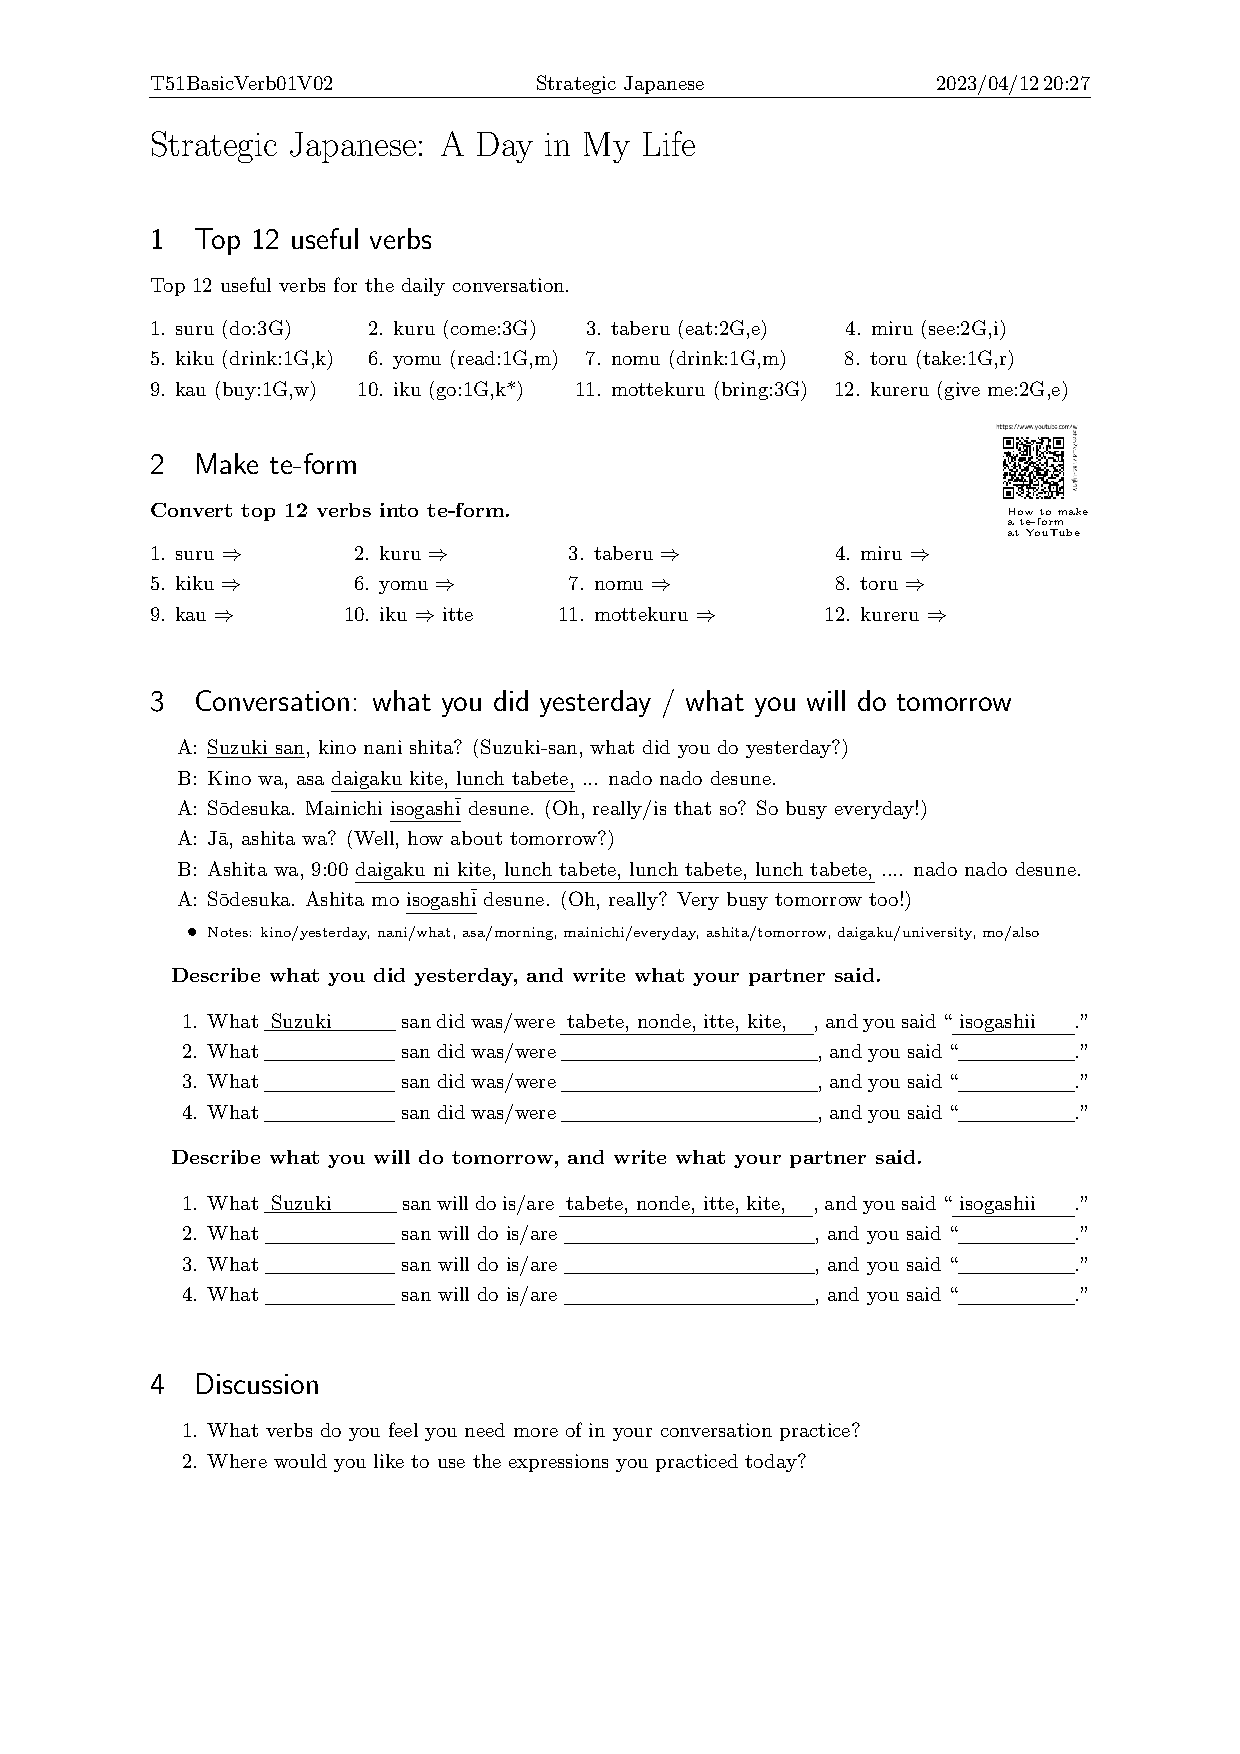
\includepdf[pages=-, scale=.86, trim=70 62 70 30, clip, offset=0mm -8.5mm, pagecommand={\thispagestyle{plain}}]{T51BasicVerb01V02.pdf}


\ifEnglish
\section{{\it Motteru?\/}(have it?)/{\it iru?\/}(need it?)}
\else
\section{持っている/要る}
\fi

%T51BasicVerb02V02.pdf: Do you want to have it? motteiru/motteinai, iru/iranai.
\ifEnglish
There are some verbs that you should pay attention to when using them.
\else
動詞の中でもいくつか使い方に注意する動詞がある。
\fi
\ifEnglish
They are four verbs which are  {\it motsu\/} (to have) and {\it iru\/} (to need) that we deal with here, and {\it aru\/} (to be), and {\it shiru\/} (to know) in the following section in Natural Speaking.
\else
ここで取り扱う「持つ」「要る」と「自然な話し方」の章で取り扱う「ある」「知る」の4つの動詞がそれである。
\fi
\ifEnglish
{\it motsu\/} and {\it iru\/} are verbs that are immediately needed in daily life.
\else
「持っている」「要る」は生活上すぐさま必要となる動詞である。
\fi
\ifEnglish
It is more often used in the form of {\it motteiru\/} (to be having) than {\it motsu\/} (to have).
\else
「持つ」よりも「持っている」の形で使われることの方が多い。
\fi
\ifEnglish
Similarly, {\it shitteiru\/} (to have known) is more often used than {\it shiru\/} (to know).
\else
同様に「知る」は「知っている」という動詞で使われることの方が多い。
\fi
\ifEnglish
However, the negative form of {\it motteiru\/} is {\it motteinai\/}, but that of {\it shitteiru\/} is {\it shiranai\/}.
\else
ところが、「持っている」の否定形は「持っていない」だが、「知る」の否定形は「知らない」である。
\fi
\ifEnglish
The negative form of {\it motteiru\/} is correctly {\it motteinai\/}, but some native speakers answer {\it motanai\/} as the answer to a question, {\it okane, motteiru\/}.
\else
「持っている」の否定形は正しくは「持っていない」であるが、母語話者の中には「お金持っている?」の答えとして「持たない」と答える人もいる。
\fi
\ifEnglish
There are another example like this. For example, {\it kono eiga, mita?\/} (Have you already seen this movie?) --- {\it Uun, minai\/} (Nope, I haven't seen it yet).
\else
このような例は他にもある。たとえば、「この映画、見た?」「ううん、見ない」がある。
\fi

\ifEnglish
The spoken word corresponding to ``need'' is not {\it hitsuyou\/} (necessary) but {\it iru\/} (to need) in Japanese.
\else
  ``need''に対応する話しことばは「必要」ではなく「要る」である。
\fi
\ifEnglish
The verb, {\it iru\/}, also means ``to want'' and is a convenient word with few syllables.
\else
「要る」は``want''の意味でもあり、音節の少ない便利な単語である。
\fi
\ifEnglish
It is commonly used in the form of {\it iru\/} and {\it iranai\/}, but there is almost no use of {\it itteiru\/}.
\else
「要る」は、「要る」「要らない」の形で普通に使われるが、「要っている」という使い方はほとんどない。
\fi
\ifEnglish
The frequency of appearance of verbs varies greatly depending on the conjugation form.
Also, since the meaning and usage of verbs changes according to the conjugation form, it is important not only to consider the meaning of the dictionary form, but to remember and use a verb in the form when it was used.
\else
動詞の出現頻度は、活用形によって大きく異なる。
また、動詞の意味や使い方は活用形にしたがって、変わるので、辞書形の意味だけを考えるのではなく、使われた時の形で覚えて、使ってみることが重要である。
\fi

\ifEnglish
\subsection {Let's learn from a simple conversation model}
\else
\subsection{とりあえず簡単な会話のモデルから学ぼう}
\fi
\ifEnglish
Only two-word questions: {\it kore motteru? kore iru?\/}
The only forms of verbs used here are {\it motteru/mottenai\/} and {\it iru/iranai\/}.
Rather than being nervous about the conjugations of complex verbs, you can just think of using such words.
\else
わずか2語の質問: これ、持ってる? これ、いる?
今ここで使う動詞の形は、「持ってる」「持ってない」「いる」「要らない」だけである。
あまり複雑な動詞の活用形に神経を使うよりも、そのような単語を使うとだけ考えればよい。
\fi
\ifEnglish
Students should do conversation practices without thinking about verb forms like this.
\else
このような言語の形を考えなくても良い会話練習を多くすべきである。
\fi
\ifEnglish
What you need to do here is to know various kinds of nouns we use together in this sentence.
\else
ここで必要なのは、この文でいっしょに使う名詞を多く知っていることである。
\fi
\ifEnglish
Try to focus on content rather than grammar.
\else
文法よりも内容を重視した活動を行うようにすることである。
\fi
\ifEnglish
Of course, the content of communication is important.
Keep it simple so that you do not have to pay attention to grammar for meaningful communication.
\else
コミュニケーションは当然、内容が重要である。
有意義なコミュニケーションを行うには、文法に注意を向けなくてもよいように、シンプルにしておく。
\fi

\begin{toiquestion}
 \ifEnglish
 Write down as many nouns as possible that you can use with verbs, {\it motteru\/} and {\it iru\/} respectively.
 \else
 「持ってる」と「要る」と共に使える名詞をそれぞれできるだけ多く書き出しなさい。
 \fi
\end{toiquestion}

\ifEnglish
The ability to speak a language is the ability to speak when not preparing.
\else
言語が話せる能力とは準備しない時の会話能力である。
\fi
\ifEnglish
If there is a preparation, it is not a language preparation, but a preparation to obtain in advance knowledge or content about what to say.
\else
もし、準備というものがあるなら、それは言語の準備ではなく、話すべきことに関する知識あるいは内容をあらかじめ知るという準備である。
\fi
\ifEnglish
Therefore, it is important to learn cultural nouns.
\else
ゆえに、文化に応じた名詞を学ぶことが重要なのである。
\fi

\ifEnglish
\subsection{Task}
First, write down the names of things you don't want.
Next, ask your friends if you need it.
\else
\subsection{タスク}
まず、自分のいらないものの名前を書き出す。
つぎに、友だちに、それが要るかどうかを聞いてみる。
\fi
\begin{toiquestion}
\ifEnglish
Write down {\bfseries things} you have and you do not need it (in English or Japanese).
\else
ほしいものを日本語でも英語でもよいので、名詞で書き出しなさい。
\fi
\end{toiquestion}

\ifEnglish
\subsection{Activity}
Ask your classmate if he/she want to have what you do not need.
\else
\subsection{活動}
自分がいらないものがいるかどうか、クラスメートに聞く。
\fi

\begin{toiquestion}
\ifEnglish
Talk to your classmates using different nouns, as in the following example.
And make a note of who needs what and what they don't need.
\else
次の例のように、いろいろな名詞を使ってクラスメートと会話しなさい。
そして、誰が何が要るか、何が要らないかメモしなさい。
\fi
\end{toiquestion}

\ifEnglish
\begin{itemize}
  \labelwidth=-10mm
  \item[You:] \underline{Suzuki} san, \underline{jitensha} motteru?
    {\tiny\hfill Suzuki san, do you have a bicycle?}
  \item[Suzuki:] Un motteru.
    {\tiny\hfill Yes, I do. I don't need it.}
  \item[You:] \underline{Tanaka} san, \underline{jitensha} motteru?
    {\tiny\hfill Tanaka san, do you have a bicycle?}
  \item[Tanaka:] Uun mottenai.
    {\tiny\hfill No, I don't.}
  \item[You:] Iru?
    {\tiny\hfill Do you want to have it?/Need it?.}
  \item[Tanaka:] Un \underline{iru}! Hoshii.
    {\tiny\hfill Yes, I need it! I want it.}
\end{itemize}
\else
\begin{itemize}
  \labelwidth=-10mm
  \item[あなた:] \underline{鈴木}さん、\underline{自転車}、持ってる?
    {\tiny\hfill Suzuki san, do you have a bicycle?}
  \item[鈴木:] うん、持ってる。
    {\tiny\hfill Yes, I do. I don't need it.}
  \item[あなた:] \underline{田中}さん、\underline{自転車}、持ってる?
    {\tiny\hfill Tanaka san, do you have a bicycle?}
  \item[田中:] ううん、持ってない。
    {\tiny\hfill No, I don't.}
  \item[あなた:] いる?
    {\tiny\hfill Do you want to have it?/Need it?.}
  \item[田中:] うん、\underline{いる}!ほしい。
    {\tiny\hfill Yes, I need it! I want it.}
\end{itemize}
\fi

\ifEnglish
\subsection{Discussion}
\else
\subsection{ディスカッション}
\fi

\begin{toiquestion}
\ifEnglish
What kind of things do you need in your daily life?
\else
日常生活で必要なものは何か。
\fi
\end{toiquestion}

\begin{toiquestion}
\ifEnglish
What words or expressions did you want to know more about during the practice?
\else
練習していてもっと知りたいと思った単語や表現は何か。
\fi
\end{toiquestion}

\begin{toianswer}
\ifEnglish
Since both {\it iru\/} (need) and {\it motteiru\/} (have) take simple sentence structures, you do not need to pay attention to grammar.
All you have to do is speak two words, a noun and a verb, in order.
Rather than that, it will be possible to promote conversation by thinking about what is necessary and what is not necessary on a daily basis.
\else
「要る」も「持っている」も簡単な文の構造であるので、文法に注意して話すことはあまりない。
単純に名詞と動詞の2つの単語を順番に話せばよいだけである。
むしろ、準備として日頃から必要なものと不要なものを考えておくことが速やかに会話をすすめることができるだろう。
\fi
\end{toianswer}

%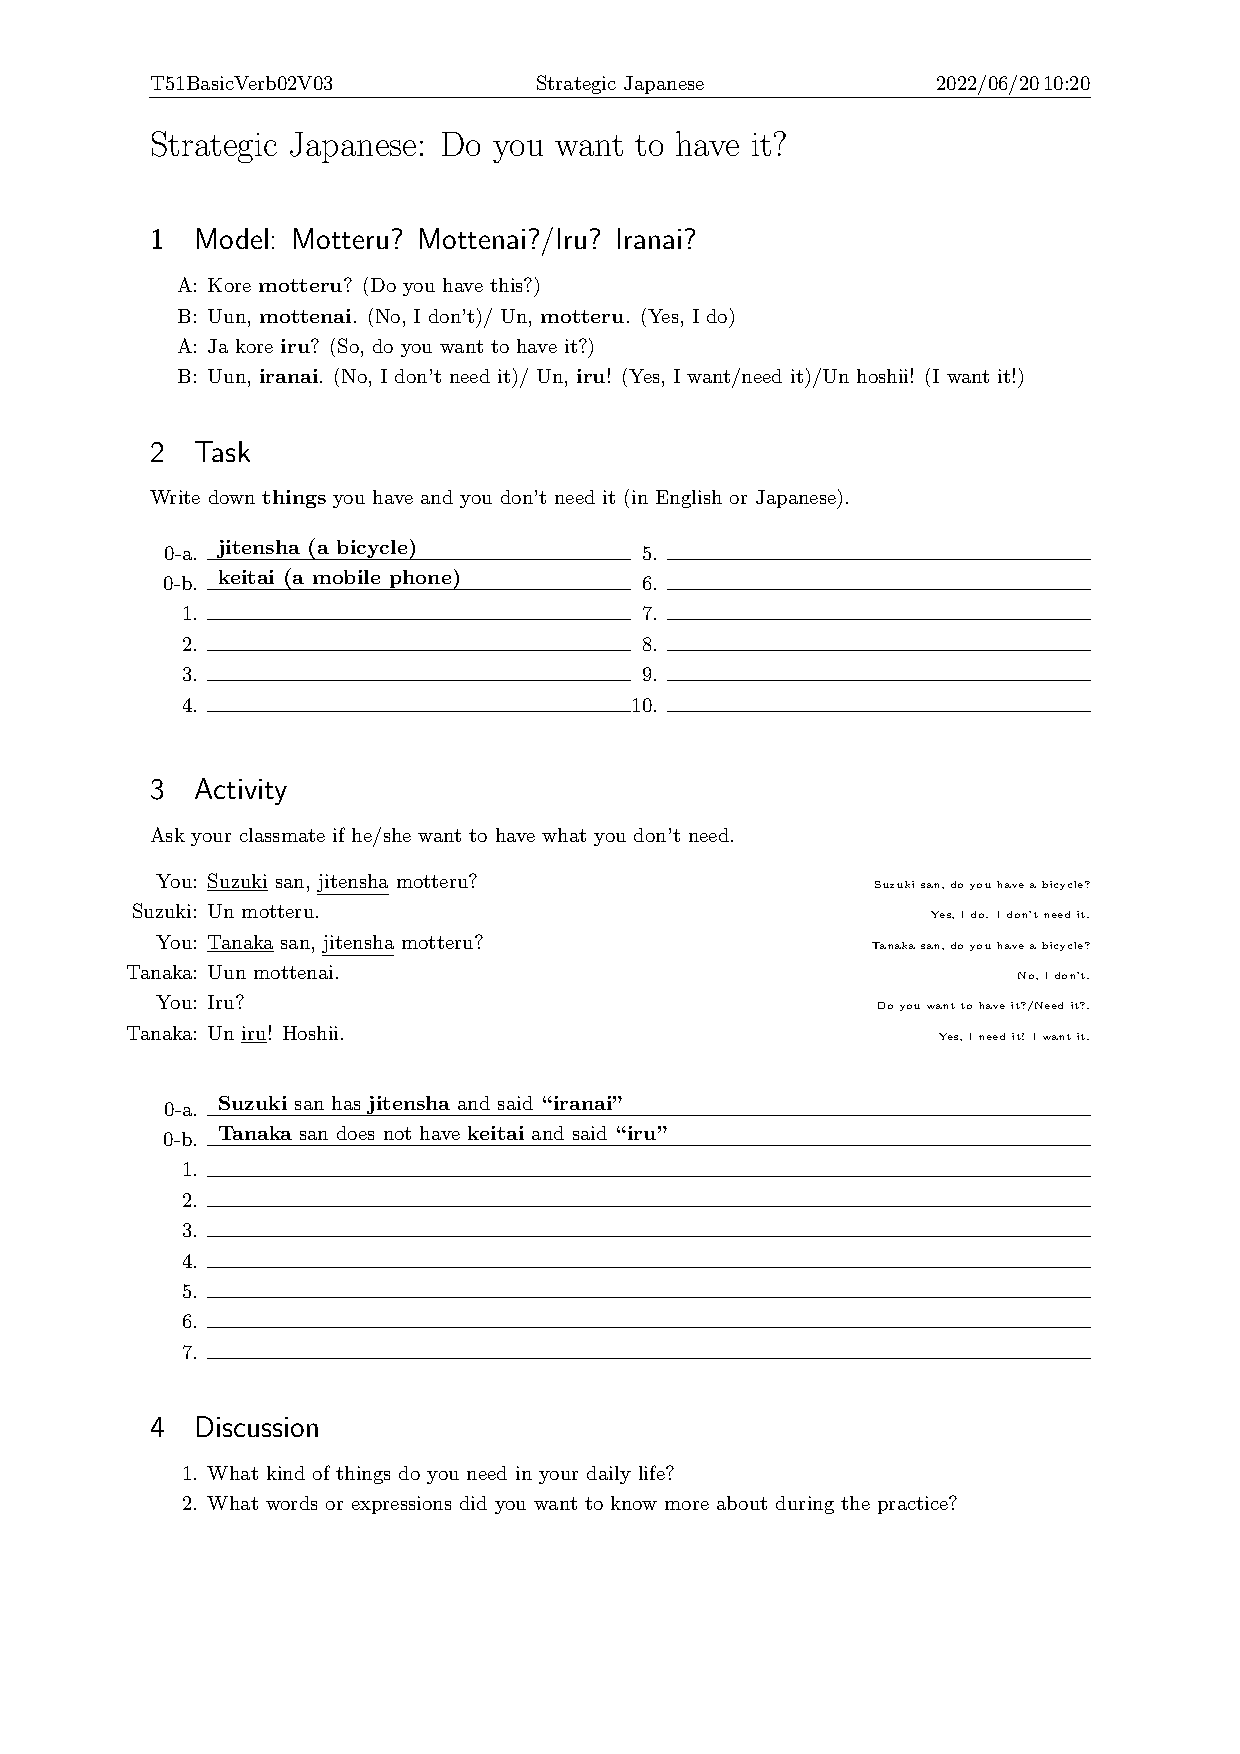
\includepdf[pages=-, scale=.86, trim=70 62 70 30, clip, offset=0mm -8.5mm, pagecommand={\thispagestyle{plain}}]{T51BasicVerb02V03.pdf}


\ifEnglish
\section{Verb negative: negative forms of verb}
\else
\section{動詞否定形}
\fi

\ifEnglish
There is an advantage in remembering the dictionary form and the negative form at the same time.
The negative form of Japanese verbs does not become a negative form only by adding something to the dictionary form.
So you have to remember the negative form for each verb.
First, if you remember the negative form, you know which group of verbs the verb belongs to.
Therefore, it is good to remember not only the dictionary form but also the negative form at the same time.
If the suffix, {\it nai} (negative auxiliary) is preceded by an a-row, the verb belongs to group I.
If not, it belongs to group II or III, but since group III includes only ``kuru'' (come) and ``suru'' (do), it is easy to see that the rest belongs to group II.
Since it is almost impossible to use verbs in actual conversation and answer immediately, it is realistic to remember each conjugation as a word.
\else
辞書形と否定形を同時に覚えるには利点がある。
日本語の否定形は、基本形に何かを付ければ、否定形になるのではない。
だから、否定形を覚えなければならない。
はじめに、否定形を覚えていれば、その動詞がどのグループの動詞なのかがわかる。
したがって、辞書形だけでなく否定形も同時に覚えるのが良い。
「ない」の前がa段であれば、Iグループ、それ以外ならIIかIIIグループだが、
IIIグループは「くる」「する」しかないので、残りはIIグループであることは容易にわかる。
実際の会話中に動詞を活用させて即答するのはほとんど不可能なので、それぞれの活用形を単語として覚えておくのが現実的である。
\fi

\begin{toiquestion}
\ifEnglish
Pronounce the Japanese verbs you know in pairs of dictionary form and negative form.
\else
知っている日本語の動詞を辞書形と否定形のペアで発音しなさい。
\fi
\end{toiquestion}

\ifEnglish
\section{Adjective: i-adjective and na-adjective}
\else
\section{イ形容詞・ナ形容詞}
\fi

\ifEnglish
\subsection{Basics}
\else
\subsection{基本}
\fi
\ifEnglish
The expressing of feelings, evaluations, and impressions is the one of the most essential speaking skills.
Adjectives are useful for conveying emotions, taste, touch, temperature, and other sensations.
Na adjectives are often used to convey reputation and reputation.
\else
感情、評価、感想を発話するのに必須。
イ形容詞は、感情や味覚、触覚、気温などの感覚を伝えるのに役に立つ。
ナ形容詞は、評価や評判を伝えるのによく使われる。
\fi
\ifEnglish
Yamato/traditional Japanese is roughly i-adjective, and Chinese and loanwords are na-adjectives, but new words may sometime be defined as i-adjectives.
\else
和語はイ形容詞、漢語や外来語はナ形容詞であるが、新しい語がイ形容詞として生まれることもある。
\fi

\begin{itemize}
  \item[A:]
    \ifEnglish
    Dou?  (How?/How do you feel?/What do you think?)
    \else
    どう?
    \fi
  \item[B:]
    \ifEnglish
    Omoshiroi/ureshii/kirei/shizuka...\\
    (It's interesting/fantastics/enjoyable/, I am happy, It's clean/beautiful,...etc.)
    \else
    おもしろい・うれしい・きれい・しずか(などなど)
    \fi
\end{itemize}

\ifEnglish
Preferences and opinions are the easiest form of expressing one's thoughts.
\else
好みや感想はもっとも簡単に自分の考えが述べられる形式。
\fi
\ifEnglish
From day one, we can have the above style of conversations.
\else
初日から、上記のような会話はできる。
\fi
\ifEnglish
Greeting is a very important conversation, but unfortunately it can't be used more than once, and doing it more than once would be strange.
\else
「あいさつ」はとても重要な会話であるが、残念ながら何回も使えないし、何回もすると奇妙である。
\fi
\ifEnglish
If you partner many conversations with a list of adjectives(\S \ref{adjectives}), you will feel like you speak naturally.
\else
形容詞のリスト(\S \ref{adjectives})を見ながら、何回もやり取りすると話した感がある。
\fi
\ifEnglish
This practice should also be done at a fast pace so as not to stagnate, and should be done like a game.
\else
この練習も停滞しないようスピードをつけて、ゲーム感覚でやるとよい。
\fi

\begin{toiquestion}
\ifEnglish
Say the following English adjectives in Japanese i-adjectives and na-adjectives.
\else
次の英語の形容詞を日本語のイ形容詞、ナ形容詞で言いなさい。
\fi
\end{toiquestion}
\begin{tabbing}
 00 \=
 00000000000000 \=
 00000000000000 \=
 00000000000000 \=
 00000000000000 \=
 00000000000000 \kill
 \>
 1. big     \>
 2. small   \>
 3. hot     \>
 4. cold    \>
 5. long  \\
 \>
 6. short  \>
 7. delicious  \>
 8. fast  \>
 9. slow  \>
\hspace{-.5em}10. famous       \\
 \>
\hspace{-.5em}11. beautiful    \>
\hspace{-.5em}12. convenient   \>
\hspace{-.5em}13. fun      \>
\hspace{-.5em}14. far      \>
\hspace{-.5em}15. strong   \\
 \>

\hspace{-.5em}16. happy    \>
\hspace{-.5em}17. noisy        \>
\hspace{-.5em}18. safety       \>
\hspace{-.5em}19. complex      \>
\hspace{-.5em}20. convenient   \\

 \>
\hspace{-.5em}21. fine         \>
\hspace{-.5em}22. easy         \>
\hspace{-.5em}23. good at      \>
\hspace{-.5em}24. dislike      \>
\hspace{-.5em}25. weak         \\

 \>
\hspace{-.5em}26. gorgeous     \>
\hspace{-.5em}27. simple       \>
\hspace{-.5em}28. kind         \>
\hspace{-.5em}29. quiet        \>
\hspace{-.5em}30. love, like   \\

\end{tabbing}

\begin{toianswer}
\ifEnglish
Use the following words.
Basically, a word ending with `i' is an i-adjective.
However, even if words end with `i', they are possibly na-adjectives, so be careful.
In the following list, na-adjectives are attached with ``/na.''
\else
つぎの単語を使う。
基本的に、語尾がiで終わる単語は、イ形容詞である。
しかし、iで終わる単語でも、ナ形容詞があるので、注意が必要である。
つぎのリストでは、ナ形容詞には語尾に/naをつけておいた。
\fi

\begin{tabbing}
 \=
 00000000000000000 \=
 00000000000000000 \=
 00000000000000000 \=
 00000000000000000 \kill

 \>
 1. ookii      \>
 2. chiisai    \>
 3. atsui      \>
 4. tsumetai   \\

 \>
 5. nagai      \>
 6. mijikai    \>
 7. oishii     \>
 8. hayai      \\

 \>
 9. osoi       \>
\hspace{-.5em}10. yuumei/na    \>
\hspace{-.5em}11. utsukushii   \>
\hspace{-.5em}12. chikai       \\

\>
\hspace{-.5em}13. tanoshii     \>
\hspace{-.5em}14. tooi         \>
\hspace{-.5em}15. tsuyoi       \>
\hspace{-.5em}16. shiawase/na  \\

\>
\hspace{-.5em}17. urusai       \>
\hspace{-.5em}18. anzen/na     \>
\hspace{-.5em}19. fukuzatsu/na \>
\hspace{-.5em}20. benri/na     \\

\>
\hspace{-.5em}21. yoi          \>
\hspace{-.5em}22. kantan/na    \>
\hspace{-.5em}23. jouzu/na     \>
\hspace{-.5em}24. kirai/na     \\

\>
\hspace{-.5em}25. yowai        \>
\hspace{-.5em}26. rippa/na     \>
\hspace{-.5em}27. kantan/na    \>
\hspace{-.5em}28. shinsetsu/na \\

\>
\hspace{-.5em}29. shizuka/na   \>
\hspace{-.5em}30. suki/na      \\

\end{tabbing}
\end{toianswer}

\ifEnglish
\subsection{Negative form}
\else
\subsection{否定形}
\fi

\ifEnglish
The negative form of the adjective is to replace the ending `i' with `kunai', and the na adjective is to add `dewanai/janai' to the end.
\else
イ形容詞の否定形は、語尾の「い」を「くない」に置き換える、ナ形容詞は、語尾に「ではない/じゃない」を付ける。
\fi

\begin{toiquestion}
\ifEnglish
Make the above i-adjectives and na-adjectives negative.
\else
上のイ形容詞、ナ形容詞を否定形にしなさい。
\fi
\end{toiquestion}
\begin{toianswer}
\ifEnglish
You can convert according to the rules mentioned above.
However, note that words ending with `i' are not always i-adjectives.
\begin{tabbing}
 \=
 00000000000000000 \=
 00000000000000000 \=
 00000000000000000 \=
 00000000000000000 \kill

 \>
 1. ookikunai      \>
 2. chiisakunai    \>
 3. atsukunai      \>
 4. tsumetakunai   \\

 \>
 5. nagakunai      \>
 6. mijikakunai    \>
 7. oishikunai     \>
 8. hayakunai      \\

 \>
 9. osokunai       \>
\hspace{-.5em}10. yuumeijanai      \>
\hspace{-.5em}11. utsukushikunai   \>
\hspace{-.5em}12. chikakunai       \\

\>
\hspace{-.5em}13. tanoshikunai     \>
\hspace{-.5em}14. tookunai         \>
\hspace{-.5em}15. tsuyokunai       \>
\hspace{-.5em}16. shiawasejanai    \\

\>
\hspace{-.5em}17. urusakunai       \>
\hspace{-.5em}18. anzenjanai       \>
\hspace{-.5em}19. fukuzatsujanai   \>
\hspace{-.5em}20. benrijanai       \\

\>
\hspace{-.5em}21. yokunai          \>
\hspace{-.5em}22. kantanjanai      \>
\hspace{-.5em}23. jouzujanai       \>
\hspace{-.5em}24. kiraijanai       \\

\>
\hspace{-.5em}25. yowakunai        \>
\hspace{-.5em}26. rippajanai       \>
\hspace{-.5em}27. kantanjanai      \>
\hspace{-.5em}28. shinsetsujanai   \\

\>
\hspace{-.5em}29. shizukajanai   \>
\hspace{-.5em}30. sukijanai      \\

\end{tabbing}
\else
上に述べたルール通りに変換すれば良い。
ただし、`i'で終わる単語は必ずしもイ形容詞ではないので注意が必要である。
\begin{tabbing}
 \=
 00000000000000000 \=
 00000000000000000 \=
 00000000000000000 \=
 00000000000000000 \kill

 \>
 1. 大きくない\>
 2. 小さくない    \>
 3. あつくない      \>
 4. つめたくない   \\

 \>
 5. nagai      \>
 6. mijikai    \>
 7. oishii     \>
 8. hayai      \\

 \>
 9. osoi       \>
\hspace{-.5em}10. yuumei       \>
\hspace{-.5em}11. utsukushii   \>
\hspace{-.5em}12. benri        \\

\>
\hspace{-.5em}13. tanoshii     \>
\hspace{-.5em}14. tooi         \>
\hspace{-.5em}15. tsuyoi       \>
\hspace{-.5em}16. shiawase/na  \\

\>
\hspace{-.5em}17. urusai       \>
\hspace{-.5em}18. anzen/na     \>
\hspace{-.5em}19. fukuzatsu/na \>
\hspace{-.5em}20. benri/na     \\

\>
\hspace{-.5em}21. yoi          \>
\hspace{-.5em}22. kantan/na    \>
\hspace{-.5em}23. jouzu/na     \>
\hspace{-.5em}24. kirai/na     \\

\>
\hspace{-.5em}25. yowai        \>
\hspace{-.5em}26. rippa/na     \>
\hspace{-.5em}27. kantan/na    \>
\hspace{-.5em}28. shinzetsu/na \\

\>
\hspace{-.5em}29. shizuka/na   \>
\hspace{-.5em}30. suki/na      \\

\end{tabbing}

\fi
\end{toianswer}


\ifEnglish
\subsection{Past form}
\else
\subsection{過去形}
\fi

\ifEnglish
The Past form of the adjective is to replace the ending `i' with `katta', and the na adjective is to add `datta' to the end.
\else
イ形容詞の過去形は、語尾の「い」を「かった」に置き換える、ナ形容詞は、語尾に「だった」を付ける。
\fi

\begin{toiquestion}
\ifEnglish
Convert the above i- and na-adjectives to the past tense respectively.
\else
上記のイ形容詞、ナ形容詞を過去形に変換しなさい。
\fi
\end{toiquestion}

\ifEnglish
  \section{How to use a particle naturally}
\else
  \section{自然な助詞の使い方}
\fi

\ifEnglish
We will learn how to use particles naturally: particles for indicating an arrival place {\it ni\/}, a mean/an action place {\it de\/}, and a leaving place {\it wo\/}.
  And the natural use of particles in a phrase; noun + particles such as {\it toshokan de benkyo\/}, {\it igirisu ni ryugaku\/}, and {\it Tokyo wo shuppatsu\/}.
\else
  助詞「に、で、を」の自然な助詞の使い方。
  それらは到着点の「に」、手段あるいは動作場所の「で」、出発点の「を」である。

  また、動詞を使わない自然な助詞の使い方も示す。
  「図書館で勉強」、「イギリスに留学」、「東京を出発」など「名詞+助詞+名詞」の形で使える。
  いずれも動作を表す名詞が後ろに置かれる。
 \fi


\ifEnglish
Figure~\ref{fig:vehicle-formation} and Figure~\ref{fig:location-formation}
indicate the cases of using particles, {\it ni\/}, {\it de\/}, and {\it wo\/}.
\else
図~\ref{fig:vehicle-formation}、図\ref{fig:location-formation}に「に」「で」「を」の使い方を示す。
\fi
\ifEnglish
Looking at both figures, you can see the concept of the three particles.
\else
両方の図を見ると、3つの助詞の持つ概念がわかるだろう。
\fi
\ifEnglish
{\it Ni\/} indicates the arrival point, {\it de\/} indicates the place of action, and {\it o\/} indicates the starting point.
\else
「に」は到着点、「で」は行為の場所、「を」は出発点を示している。
\fi
\ifEnglish
In the case of a bus, the place of the act of ``moving'' is a vehicle.
As a result, both figures represent the same concept of particles.
\else
バスの場合は、「移動」という行為の場所が乗り物である。
結果的に両方の図は同じ助詞の概念を表している。
\fi
\ifEnglish
It should be noted that when using these three particles, all of them are when using action verbs.
\else
注意しなければならないことは、これら3つの助詞を使うときは、いずれも行為を表す動詞を使うときである。
\fi
\ifEnglish
For example, {\it ni\/} may indicate an existence such as `here' or a result such as ``it will be spring.''
\else
たとえば、「に」には、「ここにあります」のような存在を示すものや、「春になります」のような結果を示すものもある。
\fi
\ifEnglish
These `ni' do not mean the arrival point.
\else
これらの「に」は到着点という意味はない。
\fi
% 20220701
\ifEnglish
In conversation, it is better to omit particles as much as possible, but when you want to distinguish the meaning, it is better to use particles explicitly.
\else
会話では、できるだけ助詞を省略するのが良いとされているが、意味を区別したいときは助詞を明示的に使った方がよい。
\fi
\ifEnglish
In the case of a verb that expresses an action, the particle cannot be omitted because the relationship between the noun and the verb that indicate the place used together in the sentence must be clearly stated.
\else
行為を表す動詞のときは、文中でいっしょに使われる場所を示す名詞と動詞との関係を明示しなければならないため、助詞を省略することができない。
\fi
\ifEnglish
Particles cannot be omitted when the meaning is difficult to understand without specifying the particles.
\else
助詞を明示しないと意味がわかりにくくなるとき、助詞は省略できない。
\fi

% 20220702
\begin{figure}[htb]\centering\small
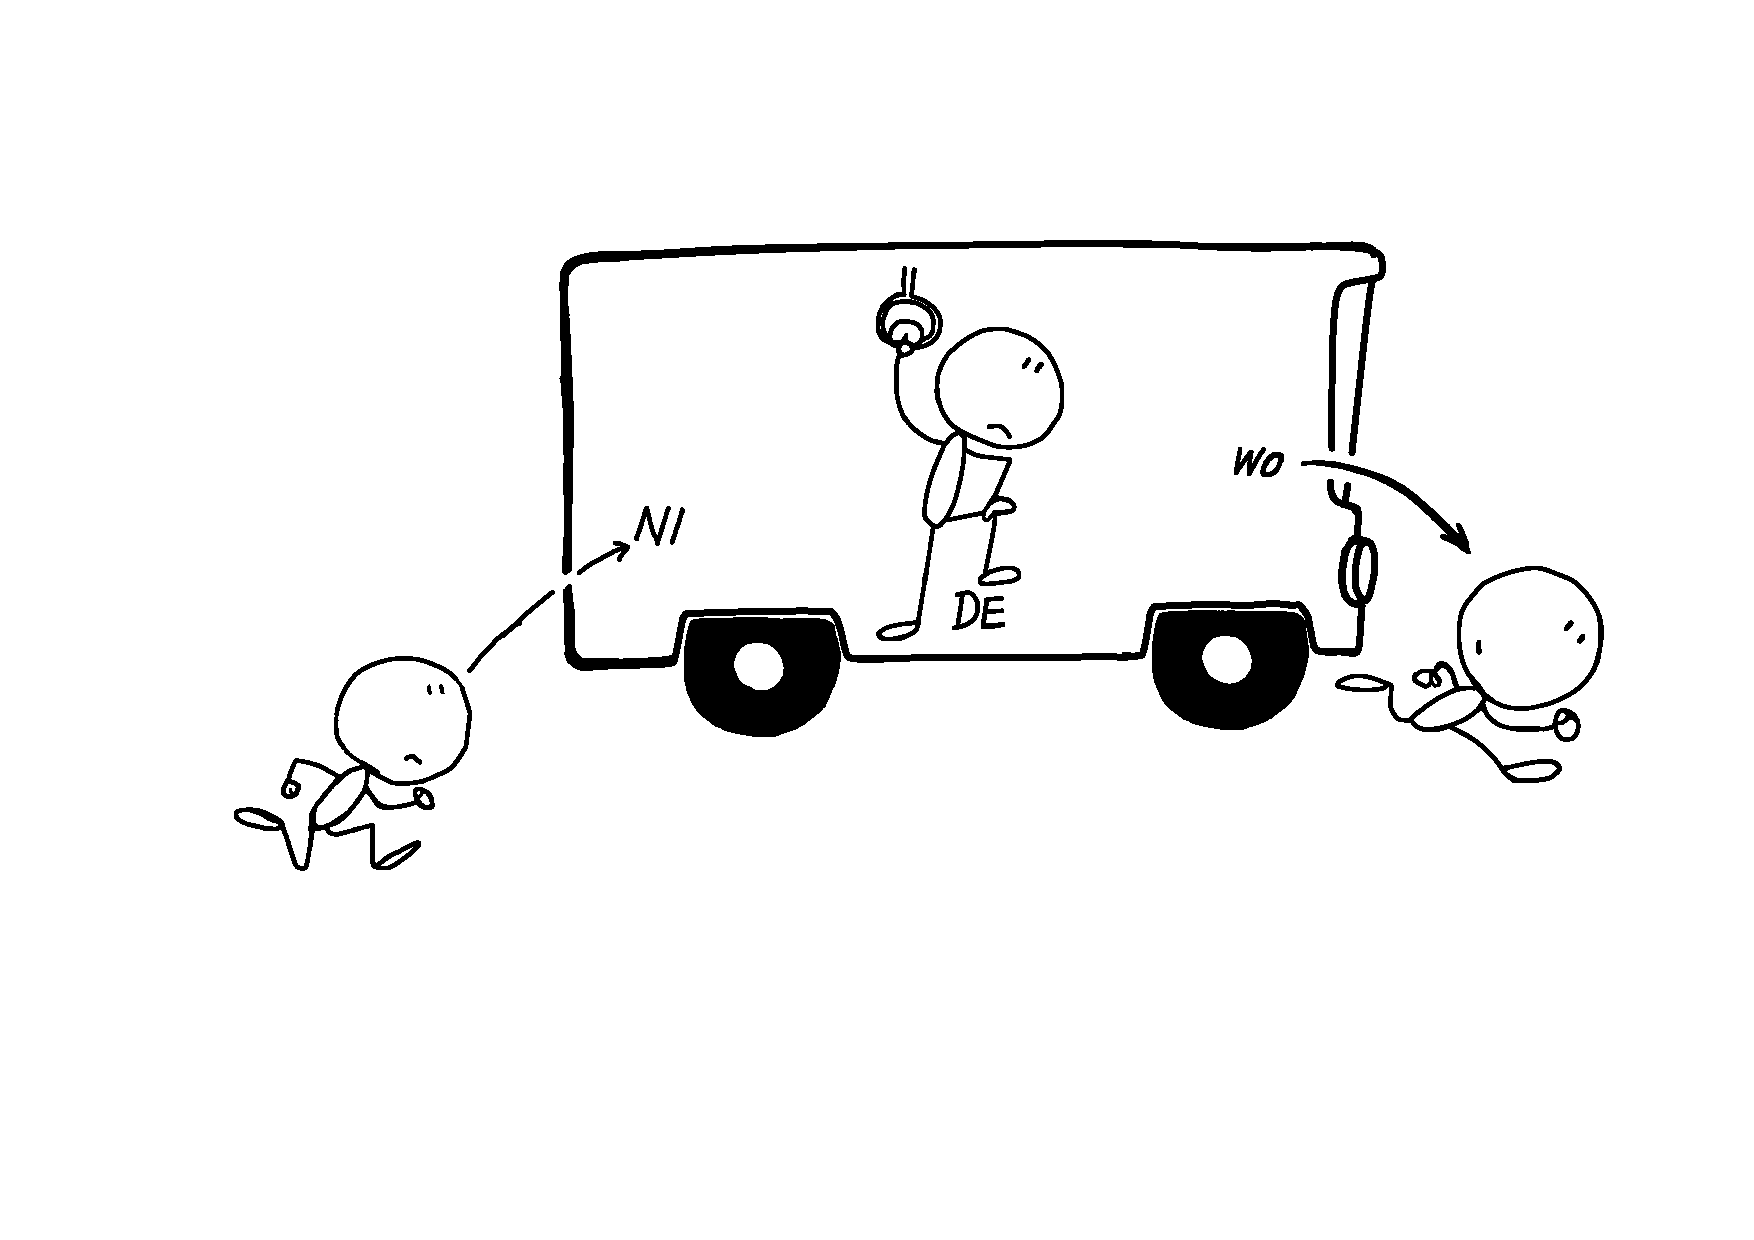
\includegraphics[trim=100 170 70 100, clip, width=.45\hsize]{subfiles/2019-06-01.pdf}
\caption{Japanese particles which have a vehicle formation}
\label{fig:vehicle-formation}
\end{figure}

\begin{figure}[htb]\centering\small
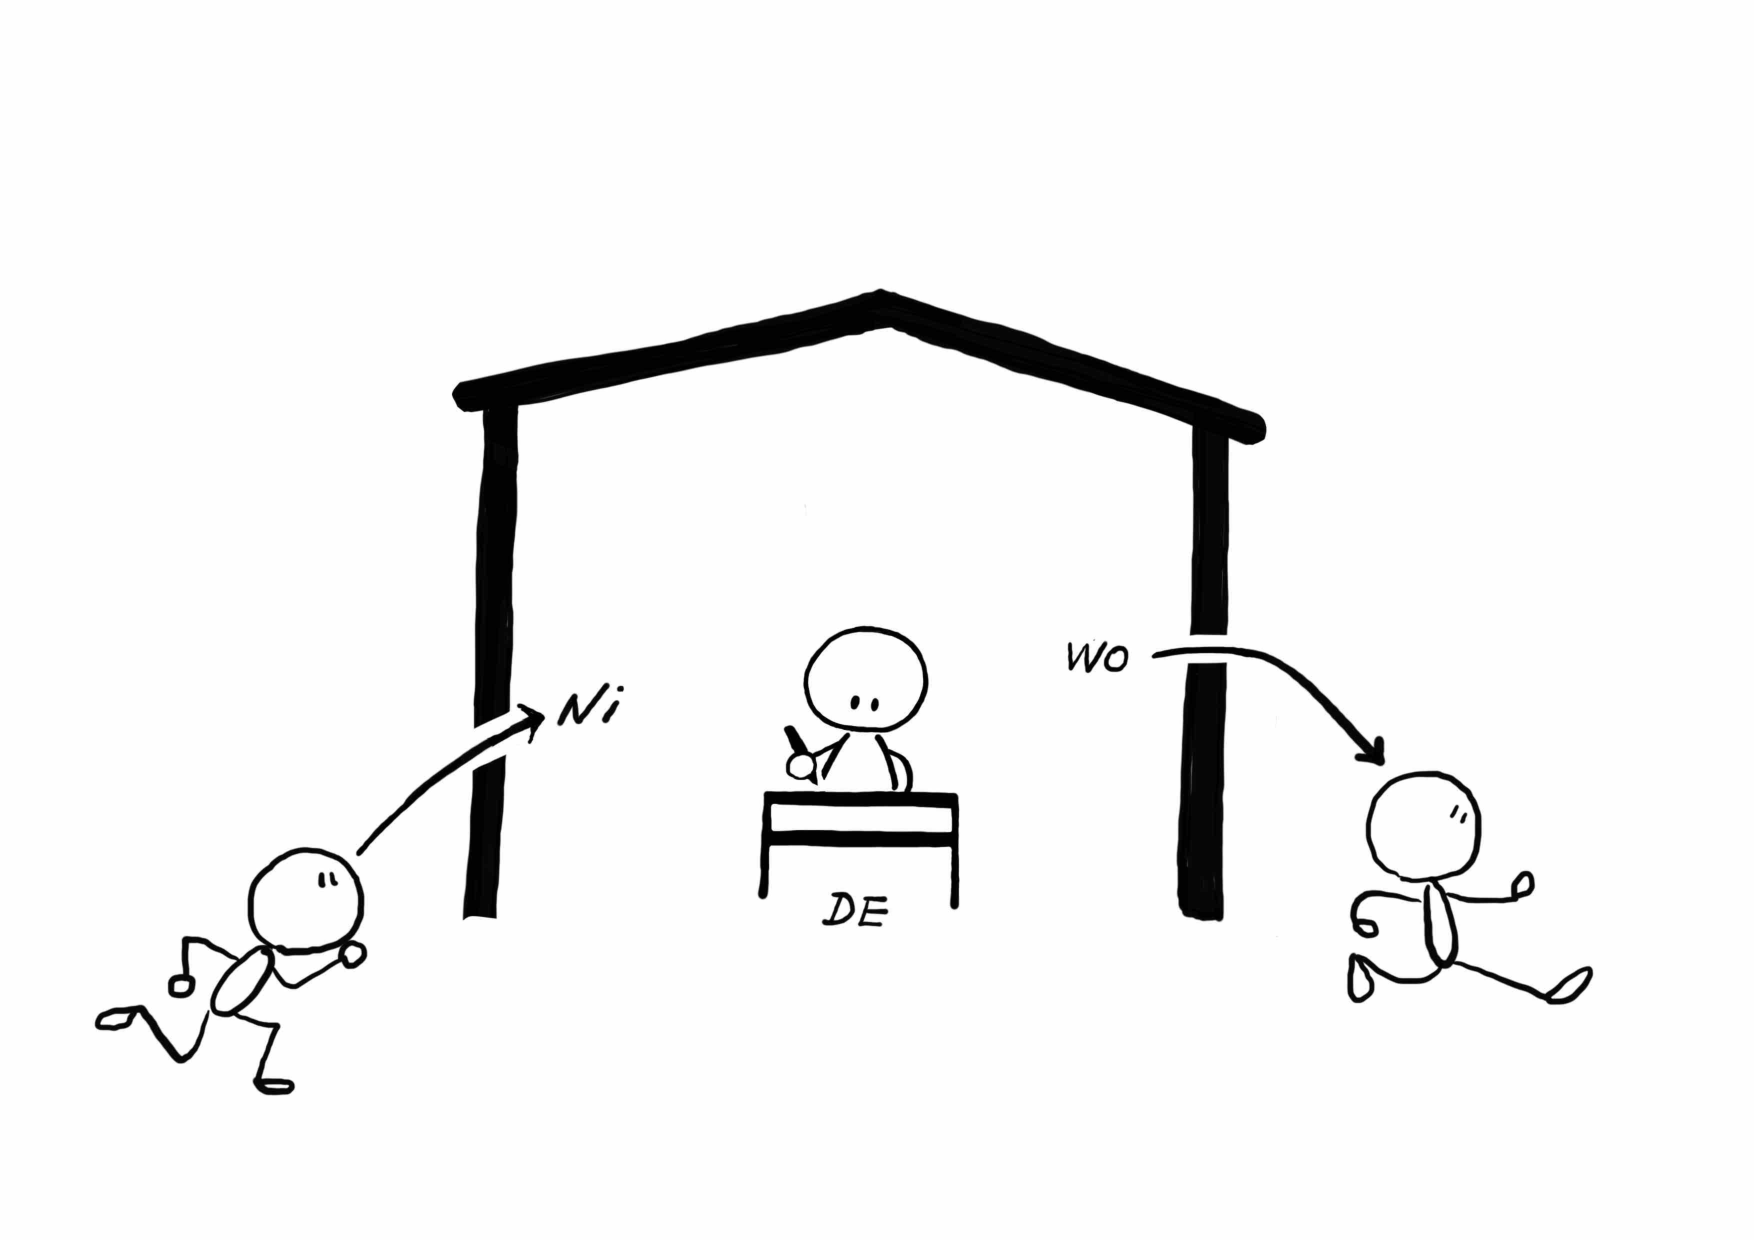
\includegraphics[trim=40 70 70 140, clip, width=.45\hsize]{subfiles/toshokan-nidewo.pdf}
\caption{Japanese particles which have a location/place formation}
\label{fig:location-formation}
\end{figure}


% 20220703
\begin{toiquestion}
\ifEnglish
Write particles that show the relationship between action verbs and nouns.
\else
行為を表す動詞と名詞の関係を示す助詞を書きなさい。
\fi
\end{toiquestion}

% 20220704
\ifEnglish
\begin{tabbing}
00000 \= 00000000000000000 \= 0000000000000000000000 \kill

\> 1. library \>
a. toshokan \underline{\hspace{2em}} iku   \\
\> \>
b. toshokan \underline{\hspace{2em}} benkyou suru\\

\> 2. bus \>
a. basu \underline{\hspace{2em}} iku   \\
\> \>
b. basu \underline{\hspace{2em}} oriru \\

\> 3. McDonald \>
a. Makudonarudo \underline{\hspace{2em}} tomodachi \underline{\hspace{2em}} ranchi suru \\
\> \>
b. Makudonarudo \underline{\hspace{2em}} biggu makku \underline{\hspace{2em}} kau \\

\> 4. home \>
a. jitaku \underline{\hspace{2em}} gozen 8 ji \underline{\hspace{2em}} deru \\
\> \>
b. jitaku \underline{\hspace{2em}} gogo 7 ji \underline{\hspace{2em}} kaeru \\

\> 5. bicycle \>
a. jitensha \underline{\hspace{2em}} daigaku \underline{\hspace{2em}} iku \\
\> \>
b. jitensha \underline{\hspace{2em}} orite aruku \\

\end{tabbing}
\else
\begin{tabbing}
00000 \= 00000000000000000 \= 0000000000000000000000 \kill

\> 1. library \>
a. 図書館\underline{\hspace{2em}} 行く   \\
\> \>
b. 図書館\underline{\hspace{2em}} 勉強する\\

\> 2. bus \>
a. バス \underline{\hspace{2em}} 行く   \\
\> \>
b. バス \underline{\hspace{2em}} 降りる \\

\> 3. McDonald \>
a. マクドナルド\underline{\hspace{2em}} 友達 \underline{\hspace{2em}} ランチする\\
\> \>
b. マクドナルド \underline{\hspace{2em}} ビッグマック \underline{\hspace{2em}} 買う \\

\> 4. home \>
a. 自宅 \underline{\hspace{2em}} 午前8時 \underline{\hspace{2em}} 出る\\
\> \>
b. 自宅 \underline{\hspace{2em}} 午後7痔 \underline{\hspace{2em}} 帰る\\

\> 5. bicycle \>
a. 自転車 \underline{\hspace{2em}} 大学 \underline{\hspace{2em}} 行く \\
\> \>
b. 自転車 \underline{\hspace{2em}} 降りて歩く \\

\end{tabbing}
\fi

\begin{toiquestion}
\ifEnglish
Practice in pairs or groups using the particle task sheet.
\else
助詞のタスクシートを使って、ペアあるいはグループで練習しなさい。
\fi
\begin{itemize}
  \item Particle 1: T51Particle01.pdf
  \item Particle 2: T51Particle02.pdf
  \item Particle 3: T51Particle03.pdf
\end{itemize}
\end{toiquestion}

\ifEnglish
As you may have noticed, the effective use of these particles can convey meaning without saying the verb at the end of the sentence.
Also, such abbreviated expressions are very natural for communication as they only state what is most necessary.
\else
もう気づいたかもしれないが、これらの助詞を効果的に用いると、文末の動詞を言わなくても意味を伝達することができる。
また、そのような省略された表現は、最も必要なことだけを述べるので、コミュニケーションとして非常に自然である。
\fi
%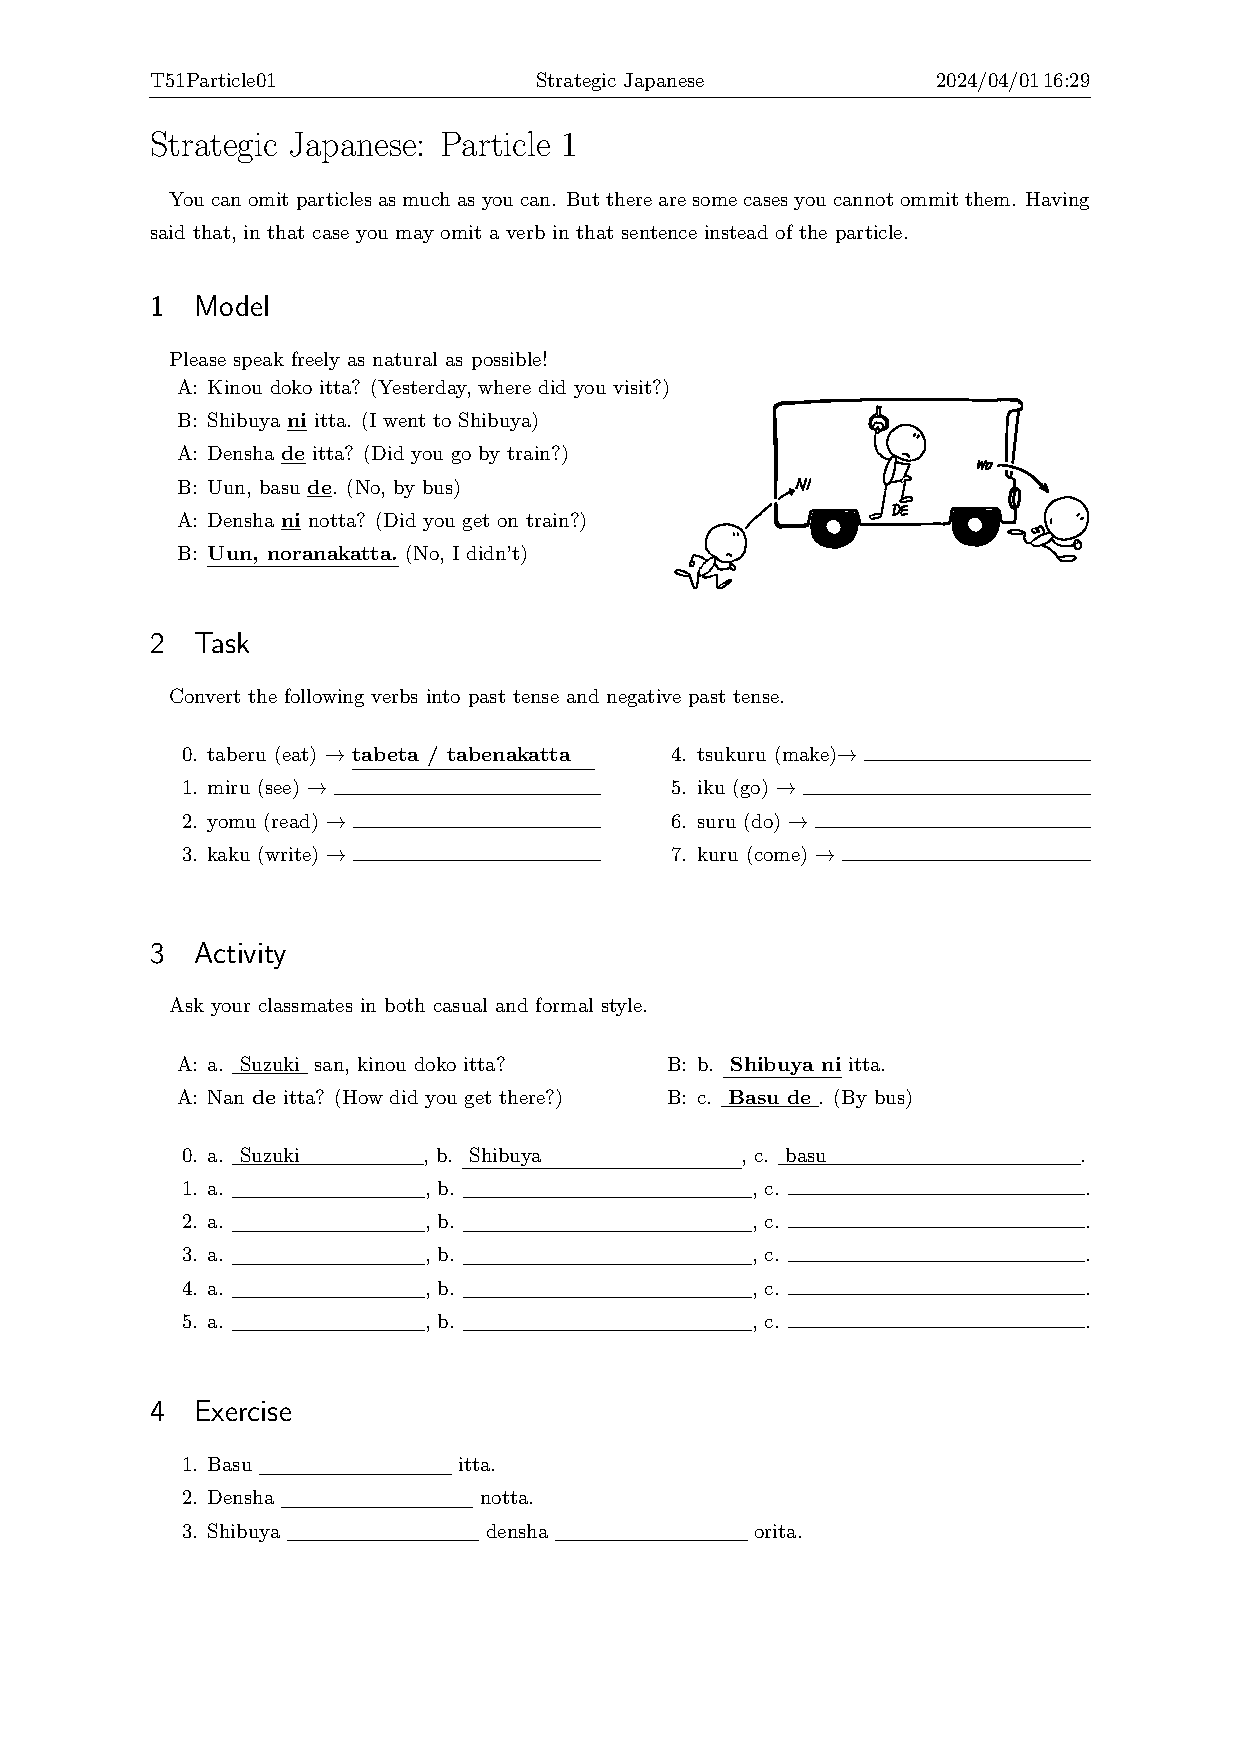
\includepdf[pages=-, scale=.86, trim=70 62 70 30, clip, offset=0mm -8.5mm, pagecommand={\thispagestyle{plain}}]{T51Particle01.pdf}
%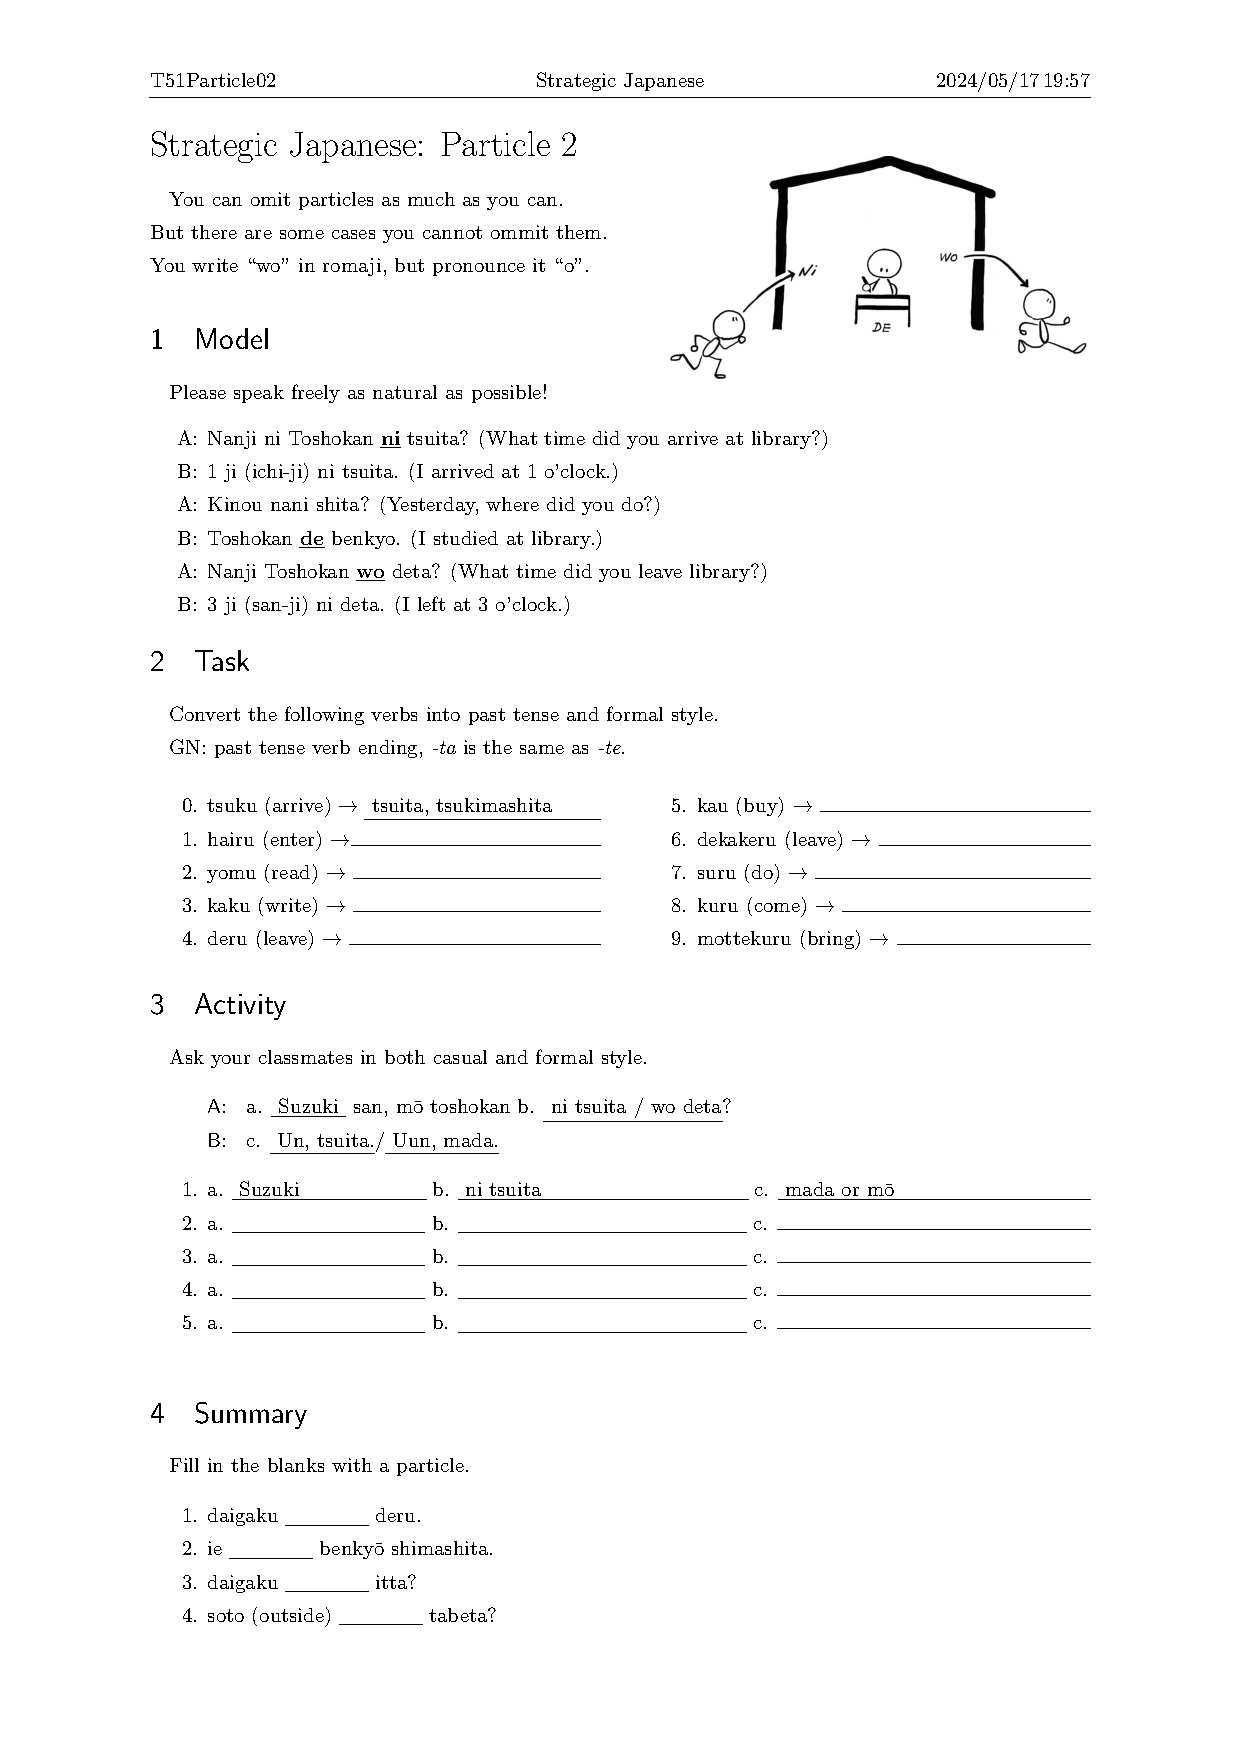
\includepdf[pages=-, scale=.86, trim=70 62 70 30, clip, offset=0mm -8.5mm, pagecommand={\thispagestyle{plain}}]{T51Particle02.pdf}
%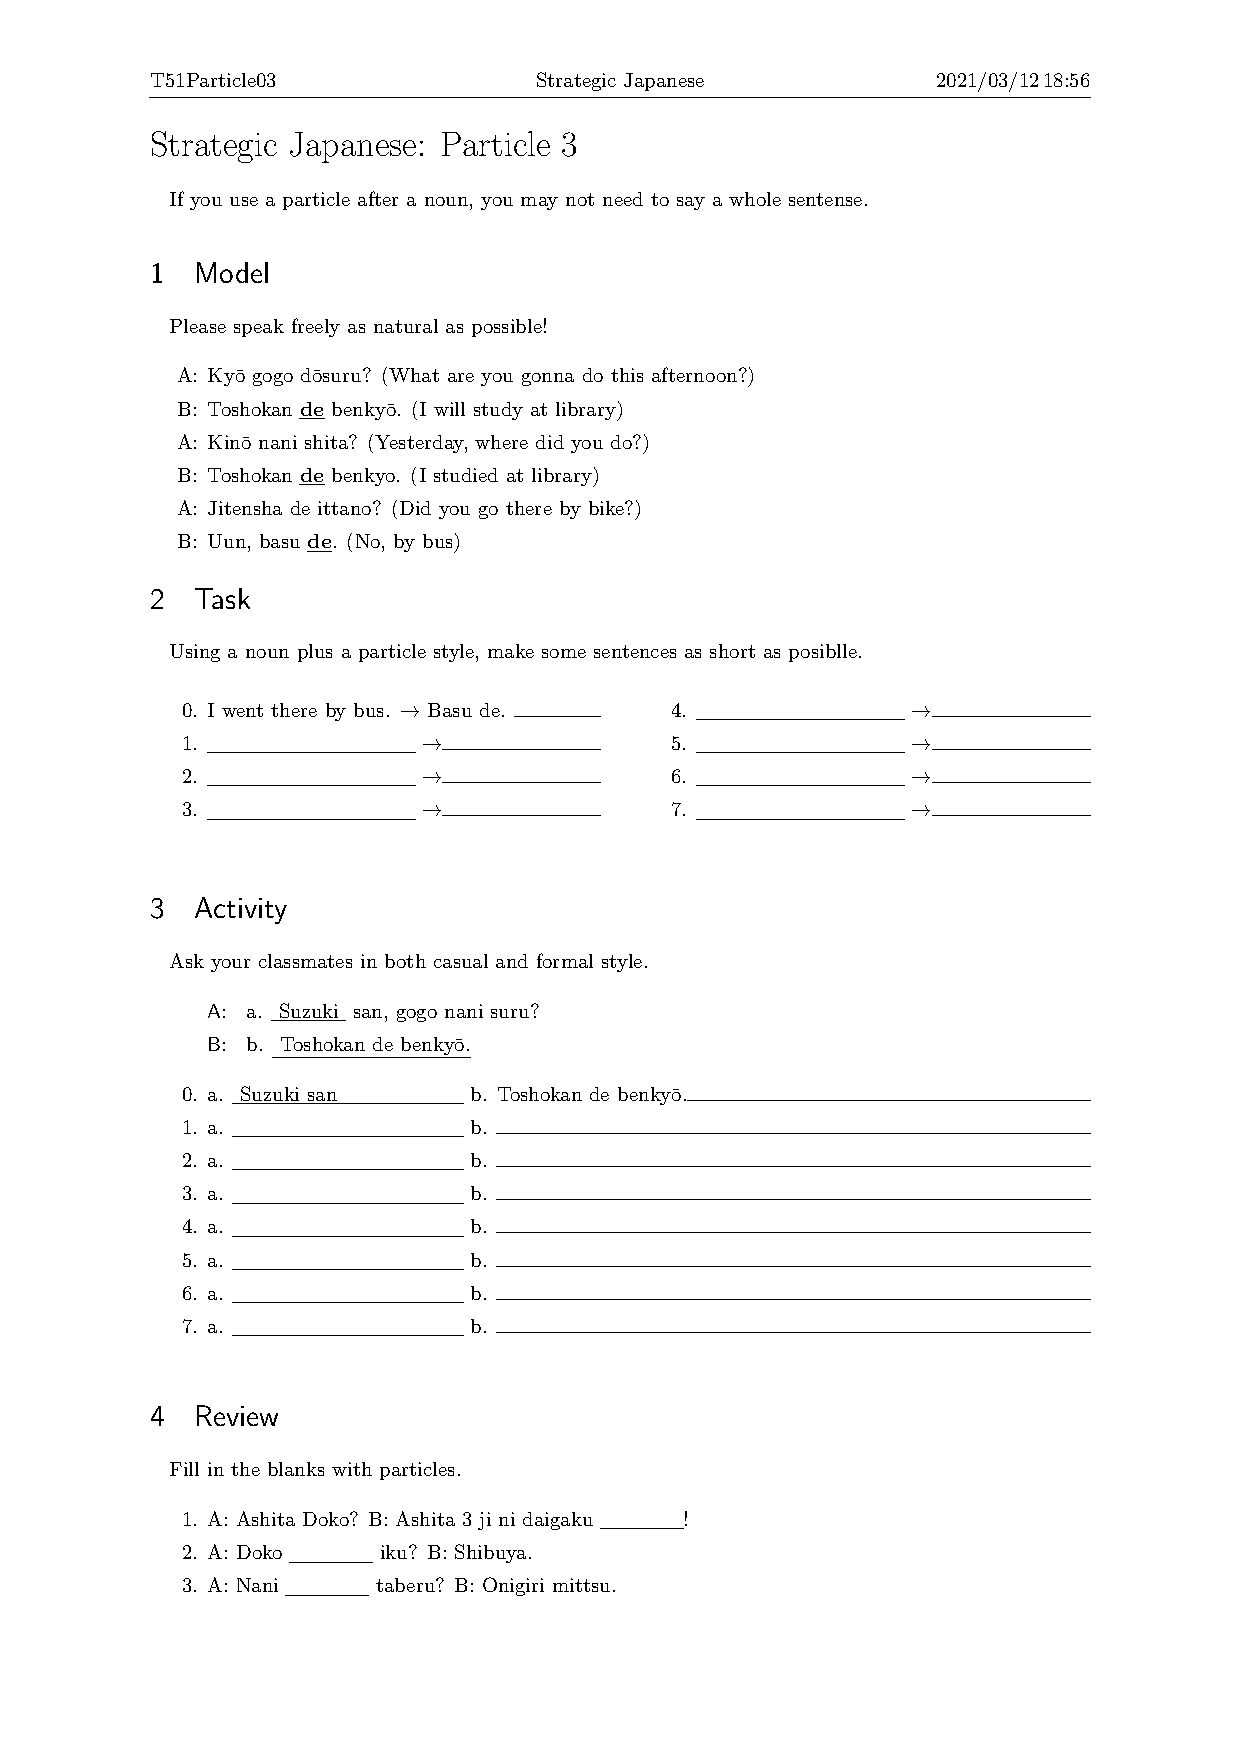
\includepdf[pages=-, scale=.86, trim=70 62 70 30, clip, offset=0mm -8.5mm, pagecommand={\thispagestyle{plain}}]{T51Particle03.pdf}

\fi%STARTFROMTHEBASICS

\ifNATURALSPEAKINGPARTONE
\ifEnglish
\chapter{Natural Speaking: Part 1}
\else
\chapter{自然に話すこと: Part 1}
\fi

\begin{abstract}

\ifEnglish
The content covered in this chapter is very important.
\else
この章で扱う内容は非常に重要である。
\fi
\ifEnglish
You will find that even short sentences can be communicated in a foreign language.
\else
短かい文でも、外国語で意思疎通が可能であることがわかるだろう。
\fi
\ifEnglish
Not only is such a short sentence easy to remember, but it also has a good rhythm, so it has the advantage of making it easy to continue interaction.
\else
このような短い文章は覚えやすいだけでなく、リズムがいいので、インタラクションを継続させやすい利点がある。
\fi
\end{abstract}

\begin{comment}
\begin{itemize}
  \item
  \ifEnglish
  Natural Speaking 1: Three words question
  \else
  自然な話し方 1: 3語で質問
  \fi

  \item
  \ifEnglish
  Natural Speaking 2: Ask something newly begun
  \else
  自然な話し方 2: 何かはじめた?
  \fi

  \item
  \ifEnglish
  Natural Speaking 3: Do you have it? / I don't know
  \else
  自然な話し方 3: 「ある」と「知らない」
  \fi

  \item
  \ifEnglish
  Natural Speaking 4: Telling an impression/feeling
  \else
  自然な話し方 4: 感想・印象・感情を話す
  \fi

  \item
  \ifEnglish
  Natural Speaking 5: Yet, already, and verb past/perfect
  \else
  自然な話し方 5: もう・まだ・過去形・完了形
  \fi

  \item
  \ifEnglish
  Natural Speaking 6: Invitation
  \else
  自然な話し方 6: 誘う・招待する
  \fi

  \item
  \ifEnglish
  Natural Speaking 7: Persuasion and reaction
  \else
  自然な話し方 7: 説得と反応
  \fi

  \item
  \ifEnglish
  Natural Speaking 8: Reporting a progressive situation
  \else
  自然な話し方 8: 進行中のことを報告する
  \fi

  \item
  \ifEnglish
  Natural Speaking 9: Potential
  \else
  自然な話し方 9: できる・ひける
  \fi

  \item
  \ifEnglish
  Natural Speaking 10: Experiences
  \else
  自然な話し方 10: 経験を話す
  \fi

  \item
  \ifEnglish
  Natural Speaking 11: Tried to do it, but..
  \else
  自然な話し方 11: 〜ようと思ったけど
  \fi

  \item
  \ifEnglish
  Natural Speaking 12: Offer advice
  \else
  自然な話し方 12: アドバイスをする
  \fi

  \item
  \ifEnglish
  Natural Speaking 13: Expressing the feeling of a regret
  \else
  自然な話し方 13: 後悔の念
  \fi

  \item
  \ifEnglish
  Natural Speaking 14: Say several reasons
  \else
  自然な話し方 14: 理由を並べて言う:
  \fi

\end{itemize}
\end{comment}

\ifEnglish
\section{Making a three-word question}
\else
\section{3語で質問}
\fi

% T51NaturalSpeaking01V03.pdf: Saikin doko itta?

\ifEnglish
You can start the topic of travel/visiting somewhere with just three words, {\it saikin doko itta\/} (where have you been recently?).
The phrase {\it saikin doko itta\/} (where have you been recently'' starts the topic of travel and visits.
\else
「最近どこ行った」という表現で、旅行・訪問のトピックが始められます。
\fi
\ifEnglish
It is a simple question in just only three words.
This is a really convenient expression.
\else
これは、たった3語で表現できる簡単な質問である。
これは実に便利な表現である。
\fi
\ifEnglish
You should relax, feel kind and talk naturally.
\else
あなたはリラックスして、優しい気持ちになって、自然に話してみてください。
\fi
\ifEnglish
It makes a natural phrase which is short and includes no particle as much as possible,
\else
できるだけ、短く、助詞を使わない文を、一息でいうと、自然な会話になる。
\fi
\ifEnglish
For the specific place name, use a word you know.
Place names are very easy to understand because they make the conversation concrete.
\else
具体的な地名は、あなたが知っている語を使えばよい。
地名は会話を具体的にするため、とても通じやすい表現になる。
\fi

\ifEnglish
Simply reply to the place name promptly.
As soon as possible, reply only with the name of the place.
Students may ask if it is rude not to use {\it desu\/} or {\it masu\/}, but since it is not necessary to express one's actions politely, it is more appropriate for communication to immediately give the answer that the other person wants rather than to reply politely.
\else
単純に地名だけを速やかに返答する。
できるだけ早く、地名だけを返答する。
学生は「です・ます」をつけないと失礼ではないかと質問するが、自分の行動を丁寧に表現する必要はないので、丁寧に返答するより、即座に相手の求める答えをする方がコミュニケーションとして適切だ。
\fi

\begin{comment}
\begin{instruction}
\ifEnglish
Task of this conversation is to note the three pieces of information: i.e., a. Interviewee's name, b. the destination, c. impressions of the place.
\else
この会話のタスクは、a.インタビュー対象者の名前、b.目的地、c.感想、の3つの情報をメモすること。
\fi
\end{instruction}

 objective
 \begin{enumerate}
  \item casual form
  \item i-adjective in non-past and past form.
  \item placenames to visit
 \end{enumerate}
\end{comment}

\ifEnglish
\subsection{Model}
\else
\subsection{モデル}
\fi

\begin{toiquestion}
\ifEnglish
Follow the model and think about what preparations you need to make to speak as naturally and freely as possible.
\else
モデルにしたがって、できるだけ自然に自由に話すには、どんな準備が必要かを考えてください。
\fi
\end{toiquestion}

\begin{description}
\ifEnglish
 \item[A:] Saikin doko itta? (Recently, where did you visit?)
 \item[B:] \underline{Shibuya (a place name)} itta! (I went to \underline{Shibuya}.)
\else
 \item[A:] 最近どこ行った?
 \item[B:] \underline{渋谷 (地名)} 行った!
\fi
\end{description}

\begin{toianswer}
\ifEnglish
To speak naturally, answer promptly when asked by the other person.
In order to answer promptly, it is necessary to prepare concrete things.
\else
自然に話すためには、相手に聞かれたら、速やかに答えることです。
速やかに答えるためには、具体的な物事を用意しておくことが必要です。
\fi
\ifEnglish
In the case of this model, the place name can be specifically prepared.
\else
このモデルの場合、具体的用意できるのは、地名です。
\fi
\ifEnglish
How many Japanese place names can you say at once?
\else
あなたは、とっさにいくつ日本の地名が言えますか。
\fi
\ifEnglish
You have to wait until the sentence pattern or expression automatically comes out of your mouth.
However, if you prepare the names of places and things in advance, you can use them immediately.
\else
文型や表現は自動的に口から出てくるまで、待たなければなりません。
しかし、地名や物の名前などは、あらかじめ準備しておけば、すぐ使えます。
\fi
\ifEnglish
Preparing to speak naturally is to learn a lot of concrete nouns, that is, to learn culture.
\else
自然に話すための準備とは、具体的な名詞を多く学ぶこと、すなわち文化を学ぶことです。
\fi
\end{toianswer}

\ifEnglish
\subsection{Task}
\else
\subsection{タスク}
\fi

\begin{toiquestion}
\ifEnglish
Write place names where you want to go.
Even if you don't have a place you want to go, write down as many place names as you know.
Write down at least 5 places you know even if you don't have any places where you want to go.
\else
行きたいところの地名を書きなさい。
行きたいところがなくても知っている地名を少なくとも5つ書きなさい。
\fi
\end{toiquestion}

\begin{enumerate}
  \item[0.] \underline{\hspace{1zw}}Shibuya\underline{\hspace{18.3zw}}
  \item \underline{\hspace{23zw}}
  \item \underline{\hspace{23zw}}
  \item \underline{\hspace{23zw}}
  \item \underline{\hspace{23zw}}
  \item \underline{\hspace{23zw}}
\end{enumerate}

\begin{toianswer}
\ifEnglish
Rather than preparing sentence patterns, it is better to prepare proper nouns.
The best way to the preparation is to consciously write down the names of places in advance.
This will help you in your listening comprehension.
What you don't understand is when you don't know the word, especially when you don't know the proper noun.
To be ignorant of proper nouns is to be ignorant of the local culture where the language is spoken.
To use language, learning culture is essential.
\else
文型を準備するよりも、固有名詞を準備したほうが良い。
準備することは、意識的に地名をあらかじめ書き出しておくことである。
聞き取りに役立つはず。
聞いてわからないのは、その語を知らない場合で、特に固有名詞を知らない場合である。
固有名詞を知らないということは、その言語の話されている地域の文化を知らないということである。
言語を使うためには、文化の学習が不可欠である。
\fi
\end{toianswer}

%\ifEnglish
%\subsection{Task B}
%\else
%\subsection{タスクB}
%\fi

\begin{toiquestion}
\ifEnglish
Choose 5 of your favorite i-adjectives.
Then write the present tense and past tense of the i-adjective.
\else
好きなイ形容詞を5つ選びなさい。
そして、そのイ形容詞の現在形と過去形を書きなさい。
\fi

\begin{enumerate}
  \item[0.] \underline{\hspace{.0zw}omoshiroi $\rightarrow$ omoshirokatta\hspace{.0zw}}
  \item \underline{\hspace{23zw}}
  \item \underline{\hspace{23zw}}
  \item \underline{\hspace{23zw}}
  \item \underline{\hspace{23zw}}
  \item \underline{\hspace{23zw}}
\end{enumerate}
\end{toiquestion}

\begin{note}
\ifEnglish
To form the past tense of i-adjectives from i-adjectives:
omoshiro\underline{i} $\rightarrow$ omoshiro\underline{katta}
\else
イ形容詞からイ形容詞の過去形を作るには、次のようにする。
おもしろ\underline{い} $\rightarrow$ おもしろ-\underline{かった})
\fi
\end{note}

\begin{toianswer}
\ifEnglish
First select a word you know and try to conjugate the past tense of that word.
Do not practice with unfamiliar words.
It is important to choose words that you like, learn from them, and use them.
\else
自分の知っている語をまず選び、その語の過去形を作ってみること。
あまり馴染みのない語で練習しないこと。
自分の好きな語を選ぶこと、その語から学習し、その語から使ってみることが重要である。
\fi
\end{toianswer}

\ifEnglish
Inflection is one of the important grammatical items to speak naturally.
This is because the conjugation is one of the words that cannot be mistaken.
You can speak the phrases in any order, but do not freely change the order of elements in a phrase.
Speaking by swapping the elements in a phrase is the same as speaking a different word.
\else
活用形は自然に話すための最も重要な文法項目の1つである。
なぜならば、活用形は言い間違いのできない語句の一つだからである。
句をどの順番で話してもよいが、句の中の要素を自由に入れ替えて話してはいけない。
句の中の要素を入れ替えて話すということは、違う語を話すのと同じことである。
\fi
\ifEnglish
But don't be afraid at all.
\else
しかし、恐れることはまったくない。
\fi
\ifEnglish
You can think of the phrase as a slightly longer noun and speak it as it is.
It should be easier than thinking, making and talking by yourself.
\else
句はちょっと長めの名詞だと見做して、そのまま話せばよい。
自分で考えて作って話すより簡単なはずである。
\fi

% 2022-07-26
\ifEnglish
\subsection{Activity}
\else
\subsection{アクティビティ}
\fi

\begin{toiquestion}
\ifEnglish
Use the following conversation pattern to ask your classmates about their recent trips.
Make a note of where and how your classmate answered.
\else
次の会話のパターンを使って、最近、行ったところについてクラスメートに聞きなさい。
クラスメートが答えた場所と感想をメモしなさい。
\fi
\end{toiquestion}

 \begin{quote}
 \begin{description}
  \item[A:] a. \underline{ Suzuki } san, saikin doko itta?
  \item[B:] b. \underline{ Shibuya } itta.
  \item[A:] \hspace*{3ex} D\={o} datta? (How was it?)
  \item[B:] c. \underline{ Omoshiro-katta (It was fun)}.
  \item[A:] S\=o, yokatta desune. (That's great!)
  \item[B:] E\=e, hontoni. (Yes, it really was!)
 \end{description}
 \end{quote}

\begin{tabular}[t]{lll}
 0 a. \underline{ Suzuki san\hspace{2.5zw}}
 & b. \underline{ Shibuya\hspace{3.9zw}}
 & c. \underline{ omoshiro-katta\hspace{2.6zw}}.\\
 1 a. \underline{\hspace{8zw}}& b. \underline{\hspace{8zw}} & c. \underline{\hspace{10zw}}.\\
 2 a. \underline{\hspace{8zw}}& b. \underline{\hspace{8zw}} & c. \underline{\hspace{10zw}}.\\
 3 a. \underline{\hspace{8zw}}& b. \underline{\hspace{8zw}} & c. \underline{\hspace{10zw}}.\\
 4 a. \underline{\hspace{8zw}}& b. \underline{\hspace{8zw}} & c. \underline{\hspace{10zw}}.\\
 5 a. \underline{\hspace{8zw}}& b. \underline{\hspace{8zw}} & c. \underline{\hspace{10zw}}.\\
% 6 a. \underline{\hspace{10zw}}& b. \underline{\hspace{10zw}} & c. \underline{\hspace{15zw}}.\\
% 7 a. \underline{\hspace{10zw}}& b. \underline{\hspace{10zw}} & c. \underline{\hspace{15zw}}.\\
\end{tabular}

\begin{toianswer}
\ifEnglish
Did you know all the place names you wrote down?
There must have been some place names you didn't know.
If you hear a place name you don't know, ask it with {\it sore, doko?\/} (where is that?).
If you don't understand the content of the conversation, you can use English from the middle of the conversation.
It is important for communication to keep the exchange of content.
\else
メモした地名をすべて知っていただろうか。
おそらく知らない地名もあったはずだ。
もし知らない地名を聞いたら、「それ、どこ」と質問しよう。
会話の内容がわからなくなったら、途中から英語を使ってもよい。
内容のやり取りを大切にすることがコミュニケーションとして重要だ。
\fi
\end{toianswer}

\ifEnglish
\subsection{Discussion}
\else
\subsection{ディスカッション}
\fi

\begin{toiquestion}
\ifEnglish
How did you feel when you were speaking naturally?
\else
自然に話している時どんな気分か。
\fi
\end{toiquestion}
\begin{toianswer} % 2022-07-27
\ifEnglish
You may have thought that you needed the reaction of the other person, that is, some facial expressions and eyes of your partners.
If you can confirm the reaction of the other person, you may have gained confidence.
Once you were confident, you would have been able to relax naturally.
You would have had time and time to think about what to say next.
\else
相手の反応、すなわち、表情や目線が必要だと思ったかもしれない。
相手の反応が確認できたら、自信が生まれてきたかもしれない。
自信が生まれてきたら、自然とリラックスできただろう。
次に何を言うかを考える時間や余裕も生まれてきただろう。
\fi
\end{toianswer}

\begin{toiquestion}
\ifEnglish
What is the point of how to speak naturally?
\else
自然な話し方のポイントは何か。
\fi
\end{toiquestion}
\begin{toianswer} % 2022-07-27
\ifEnglish
Have you ever tried to speak accurately, talking too long, speaking slowly, or delaying your response?
To speak naturally, do the exact opposite.
Do not try to speak accurately, speak as you think. Speak in the order you want to say.
speak as short as possible.
When asked, reply immediately.
This way, you will uncontiously speak out important things first.
It is important to talk about the important things first.
\else
正確に話そうと考えるあまり、長く話したり、ゆっくり話したり、返答が遅れたりすることは経験ないだろうか。
自然な話し方をするには、まったくその逆を実践すればよい。
正確に話そうとせず、思ったまま話す。思った順に話す。
できるだけ短かく話す。
聞かれたら、すぐに返答する。
こうすることで、あなたは無意識に重要なことから先に発話することになる。
重要なことを先に話すことが重要である。
\fi
\end{toianswer}

\begin{toiquestion}
\ifEnglish
What kind of techniques or words can you add to improve your speech?
\else
もっとうまく話すためにどんな技術や語を付け加えたらよいか。
\fi
\end{toiquestion}

\begin{toianswer}
\ifEnglish
It's normal to want to speak a little better.
Try using only one word that you intuitively want to say.
The point is not to remember many things at a time, but to remember only one.
\else
もう少し上手に話したいと思うのは普通である。
直感的に自分が言いたいと思った単語を1つだけ使ってみること。
急にたくさんのことを覚えるのではなく、1つだけ覚えるのがポイントである。
\fi
\end{toianswer}

%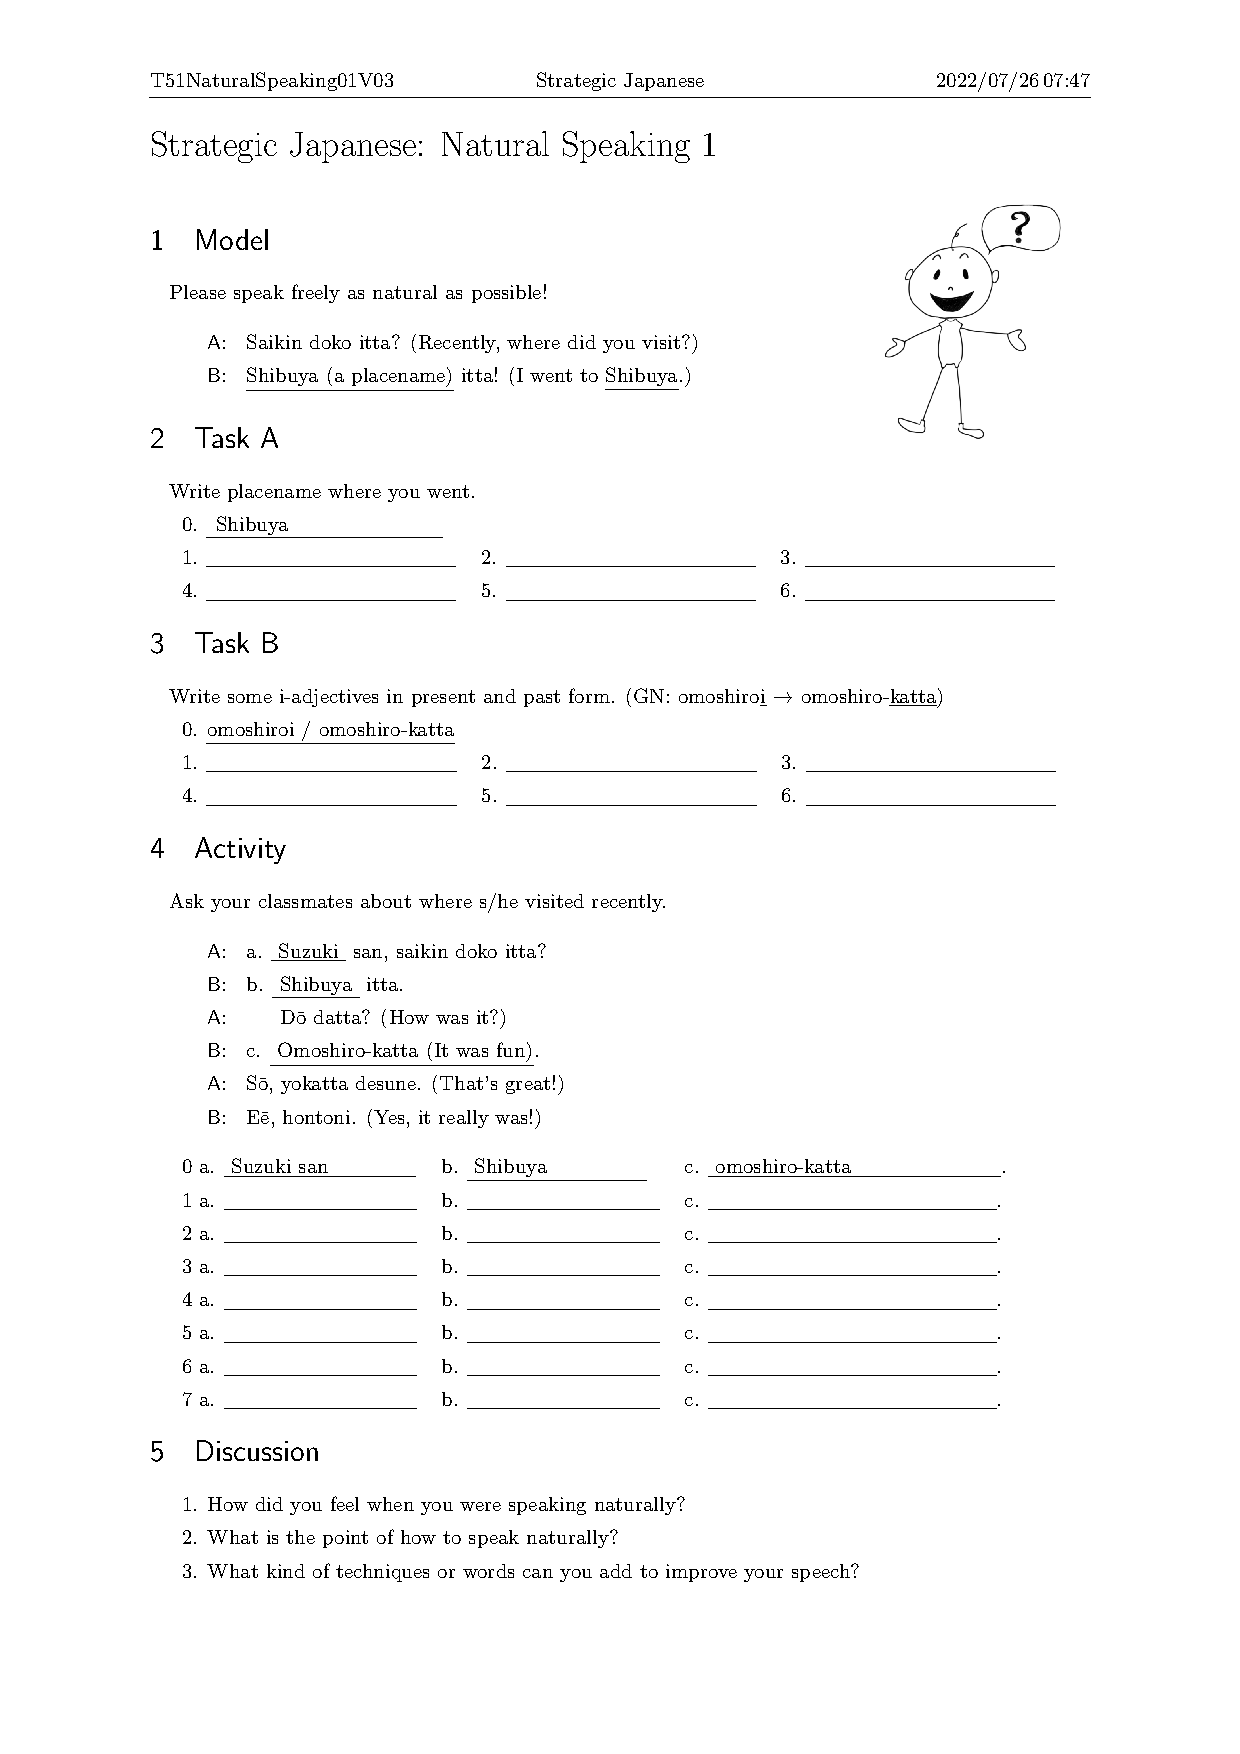
\includepdf[pages=-, scale=.86, trim=70 62 70 30, clip, offset=0mm -8.5mm, pagecommand={\thispagestyle{plain}}]{T51NaturalSpeaking01V03.pdf}
%\includepdf[pages=-, scale=.86, trim=70 62 70 30, clip, offset=0mm -8.5mm, pagecommand={\thispagestyle{plain}}]{T51NaturalSpeaking01V02.pdf}
% \item Ask students to bring a clip board. Task A: Write placename where you went; Task B: Write some adjectives in past or present form.

\ifEnglish
\section{Ask something newly begun}
\else
\section{何かはじめた?}
\fi

\ifEnglish
Natural Speaking 2 shows expressions, {\it Nanika hajimeta?\/}, {\it J\=ud\=o hajimeta\/}, {\it J\=ozu ni natta?\/}, {\it Iie, madamada\/}.
\else
Natural Speaking 2 では、「最近、何か始めた?」「柔道始めた」「上手になった」「いいえ、まだまだ」などの表現を示す。
\fi
\ifEnglish % 2022-07-29
Getting started is not as easy as it sounds.
\else
話を始めるのは思っているほど簡単なことではない。
\fi
\ifEnglish
Especially in new relationships, we know very little about the other person.
What topic should we start with?
\else
特に新しい人間関係では、相手のことをほとんど知らない。
どんなトピックから話を始めればよいのだろうか。
\fi
\ifEnglish
In the past, I could easily ask about my family and work, but nowadays it's about privacy, so it may not be an appropriate topic.
\else
かつては、家族のこと、仕事のことも気軽に尋ねることもできたが、最近はプライバシーに関わることなので、適切なトピックではないかもしれない。
\fi
\ifEnglish
As a safe topic, it may be a good idea to ask if you have a hobby that you recently started.
\else
無難なトピックとして、最近始めた趣味があるかどうかを尋ねるのはよいかもしれない。
\fi

\ifEnglish
Even if you have not started recently, it is a good idea to answer what you are doing as a hobby.
At that time, it is good to say, {\it .... yatteru\/} such as {\it Judo yatteru\/}.
\else
もし、最近始めたことがなくても、何か趣味としてやっていることを答えるのがよいアイデアだろう。
そのときは、「柔道、やっている」のように何かすでにやり始めていることを言うとよいだろう。
\fi
\ifEnglish
Even if you can do it well, you should answer that you are not doing it well at first.
\else
上手であったとしても、最初はあまり上手ではないと答えるとよい。
\fi
\ifEnglish
Don't start out boasting.
It is better to show that you are good at something after you have gotten to know each other.
\else
自慢をはじめからしない。
仲良くなってから、上手であることを見せるのがよい。
\fi
\ifEnglish
At first, it is better to be humble and say, {\it No, no\/}.
However, if you are asked to do it, you don't have to do it poorly on purpose.
\else
はじめは「いえいえ」といって謙遜したほうが良い。
しかし、「やってみて」と言われたら、わざと下手にする必要はない。
\fi

\ifEnglish
\subsection{Model}
\else
\subsection{モデル}
\fi

\begin{toiquestion}
\ifEnglish
Have you seen, heard, or spoken in your native language a scene or conversation similar to the model?
Share your experience with your group members if you have.
\else
自分の母語でモデルに似た場面や会話を見たり、聞いたり、話したりした経験があるか。
あればその経験を共有しなさい。
\fi
\end{toiquestion}

\begin{itemize}
 \item[A:]
   \ifEnglish
  Saikin, nani ka hajimeta?
  supo-tsu toka, shumi toka, nanka ... \\
  (Recently, did you start something?, sports or hobbies or ..)
   \else
   最近、何か、始めた?スポーツとか、趣味とか、なんとか...
   \fi
 \item[B:]
   \ifEnglish
   \underline{ A } hajimeta! (I have just begun \underline{{\bfseries to do A}}.)
   \else
   \underline{ A } はじめた!
   \fi
 \item[A:]
   \ifEnglish
   Dou? (How's goin'?)
   \else
   どう?
   \fi
 \item[B:]
   \ifEnglish
   Iie madamada (I cannot do it well/cool yet).
   \else
   いいえ、まだまだ。
   \fi
\end{itemize}

\begin{note}
\ifEnglish
{\it nani ka\/} v.s. {\it nani ga\/}: ``something'' vs ``what is.''
\else
何か(something)と何が(what is)
\fi
\end{note}

\begin{toianswer}
\ifEnglish
You may have similar experiences in your native language.
\else
あなたの母語においても同様の経験はあるだろう。
\fi
\ifEnglish
Think back to some of your experiences and imagine what kind of response or reaction you might receive from the other person.
\else
その経験を思い出して、相手からどんな答や反応があるだろうかを想像しなさい。
\fi
\ifEnglish
If you can remember your own past experiences, you will feel a little less nervous and easier to talk about.
\else
あなた自身が持っているかつての経験を思い出すことができれば、少し緊張がほぐれて話しやすくなるだろう。
\fi
\ifEnglish
At the beginning,
you may explicitly use the following words and phrases with your sentences:
atarashiku (newly), saikin (recently), korona ni natte (it becomes Covid-19)...
\else
冒頭で、「新しく」「最近」「コロナになって」などの語句を明示的に使っても良い。
\fi
\ifEnglish
{\it Atarashiku\/} is the adverb form of i-adjective {\it atarashii\/}, replacing the ending {\it i\/} with {\it ku\/}.
\else
「新しく」はイ形容詞「新しい」の副詞形で、語尾の「い」を「く」に置き代えたもの。
\fi
\end{toianswer}

\ifEnglish
\subsection{Task}
\else
\subsection{タスク}
\fi

\begin{toiquestion}
\ifEnglish
Make a note of what you started, such as hobbies, sports, studies, habits, etc.
\else
趣味、スポーツ、勉強、習慣など、はじめたことをメモしなさい。
\fi
\end{toiquestion}

\begin{toianswer} % 2022-08-02
\ifEnglish
Having nouns ready makes it easier to speak.
Here are some examples.

Example) cooking, soccer, guitar, jogging, yoga, calligraphy, judo, kendo, tea ceremony, etc.
\else
名詞を準備しておくことで発話しやすくなる。
いくつか例を挙げる。

例) 料理、サッカー、ギター、ジョギング、ヨガ、習字、柔道、剣道、茶道、など。
\fi
\end{toianswer}

\begin{toiquestion}
\ifEnglish
Think about what it means to be successful.
\else
「上手になった」というのはどういう意味か、考えよ。
\fi
\end{toiquestion}

\begin{toianswer}
\ifEnglish
{\it Naru\/} in the expression ``getting better'' indicates change.
{\it Jouzu\/} is a na-adjective, and when it is connected to the verb {\it naru\/} that expresses change, {\it ni\/} is added, as in {\it jouzu ni\/}.
\else
「上手になった」という表現の中の「なる」は変化を表わす。
「上手」はナ形容詞であり、変化を表わす動詞「なる」と接続するときには、「上手に」のように「に」を付ける。
\fi
\end{toianswer}

\ifEnglish % 2022-08-03
\subsection{Activity}
\else
\subsection{アクティビティ}
\fi

\begin{toiquestion}
\ifEnglish
Ask your classmates what s/he has just begun.
\else
何をはじめたかをクラスメートに聞く場面である。
\fi
\ifEnglish
Speak as naturally and freely as possible according to the following model.
\else
次のモデルにしたがって、できるだけ自然に自由に話しなさい。
\fi
\ifEnglish
When you are the listener, follow the example and take notes.
\else
あなたが聞き手のときは、例にならってメモを取りなさい。
\fi
\end{toiquestion}

\begin{quote}
\begin{description}
 \item[A:] a. \underline{ Yamamoto } san, nani ka hajimeta? supo-tsu toka, shumi toka, nanika...
 \item[B:] b. \underline{ furansugo }.
 \item[A:] J\={o}zu ni natta? (Did you do it well?/Has it become good?)
 \item[B:] c. \underline{ iie, madamada. / ee, m\={a} / ee, m\={a}m\={a}}. (No, not yet!/So so..)
\end{description}
\end{quote}

\begin{tabular}[t]{lll}
 0. a. \underline{ Yamamoto san\hspace{0.7zw}}
 &  b. \underline{ furansugo\hspace{3.0zw}}
 &  c. \underline{ iie, madamada\hspace{4.8zw}}.\\
 1. a. \underline{\hspace{8zw}}& b. \underline{\hspace{8zw}} & c. \underline{\hspace{12zw}}.\\
 2. a. \underline{\hspace{8zw}}& b. \underline{\hspace{8zw}} & c. \underline{\hspace{12zw}}.\\
 3. a. \underline{\hspace{8zw}}& b. \underline{\hspace{8zw}} & c. \underline{\hspace{12zw}}.\\
 4. a. \underline{\hspace{8zw}}& b. \underline{\hspace{8zw}} & c. \underline{\hspace{12zw}}.\\
 5. a. \underline{\hspace{8zw}}& b. \underline{\hspace{8zw}} & c. \underline{\hspace{12zw}}.\\
\end{tabular}

\begin{toianswer}
\ifEnglish
It can be a language study, like French, German, or Chinese, or it can be a hobby, a study, or a new habit.
\else
フランス語、ドイツ語、中国語のように語学でもよいし、趣味や研究や新たな習慣でもよい。
\fi
\end{toianswer}


\ifEnglish
\subsection{Discussion}
\else
\subsection{ディスカッション}
\fi

\begin{toiquestion}
\ifEnglish
Discuss what a useful topic is to start talking about other than the model.
\else
モデル以外に話を始めるのに便利なトピックを議論しなさい。
\fi
\end{toiquestion}
\begin{toianswer}
\ifEnglish
It's harder than we thought to find a topic to start talking about.
It is a good idea to always think of a topic that is suitable for starting a conversation, and check words related to that topic.
On the other hand, hearing is also difficult because you don't know what will be said.
Therefore, if you speak from yourself and are asked a question by the other person, you can tell what you have prepared in advance.
\else
話を始めるトピックは思ったより見つからない。
常日頃から会話開始にふさわしいトピックを考えておくこと、そのトピックに関連する語を調べておくとよい。
一方、聞き取りも何が言われるかわからないので、やはりこれも難しい。
だから、自分から発話して、相手に質問してもらえば、あらかじめ準備していたことを話すことができる。
\fi
\end{toianswer}


%% 2022-08-01
\ifEnglish
\subsection{Supplementary practice}
\else
\subsection{補足練習}
\fi

\begin{toiquestion}
\ifEnglish
Write things or actions you cannot do yet.
\else
まだできないことをメモしなさい。
\fi
\end{toiquestion}
\begin{toianswer}
\ifEnglish
Japanese, swimming, driving a car, kanji, playing the piano, and many other things you can't do.
\else
日本語、水泳、車の運転、漢字、ピアノなど、できないことはいろいろあるだろう。
\fi
\end{toianswer}

\begin{toiquestion}
\ifEnglish
Use noun + {\it dekiru\/} (can) and noun + {\it dekinai\/} (cannot) to state what you can and can't do.
\else
名詞+「できる」、名詞+「できない」を使って、できることとできないことを述べてみよう。
\fi
\end{toiquestion}
\begin{toianswer} % 2022-08-13
\ifEnglish
When asking a question, just ask, {\it Ryori dekiru?\/} (Can you cook?)
When answering, just say {\it dekiru\/} (I can) or {\it dekinai\/} (I can't).
Cooking, driving, swimming, mental arithmetic, jump rope, kendama, juggling, etc. It would be useful to know many words that can be expressed with nouns + {\it dekiru/dekinai\/}.
It is useful to remember how to say what you can do, such as {\it iroiro dekiru\/} (I can do many things), {\it nanimo dekinai\/} (I can't do anything), {\it yoku dekiru\/} (I can do it well), {\it zenzen dekinai\/} (I can't do anything at all), {\it maamaa dekiru\/} (I can do it to some degree), {\it sukoshi dekiru\/} (I can do a little), etc.
\else
質問するときは、「料理、できる?」と聞けばよい。
答えるときは、「できる」あるいは「できない」とだけ言えばよい。
料理、運転、水泳、暗算、縄跳び、けん玉、ジャグリングなど名詞+できる/できない、で表現できる語を多く知っておくと役に立つだろう。
いろいろできる、何にもできない、よくできる、ぜんぜんできない、まあまあできる、少しできる、など、できる程度の言い方を覚えておくと便利である。
\fi
\end{toianswer}

%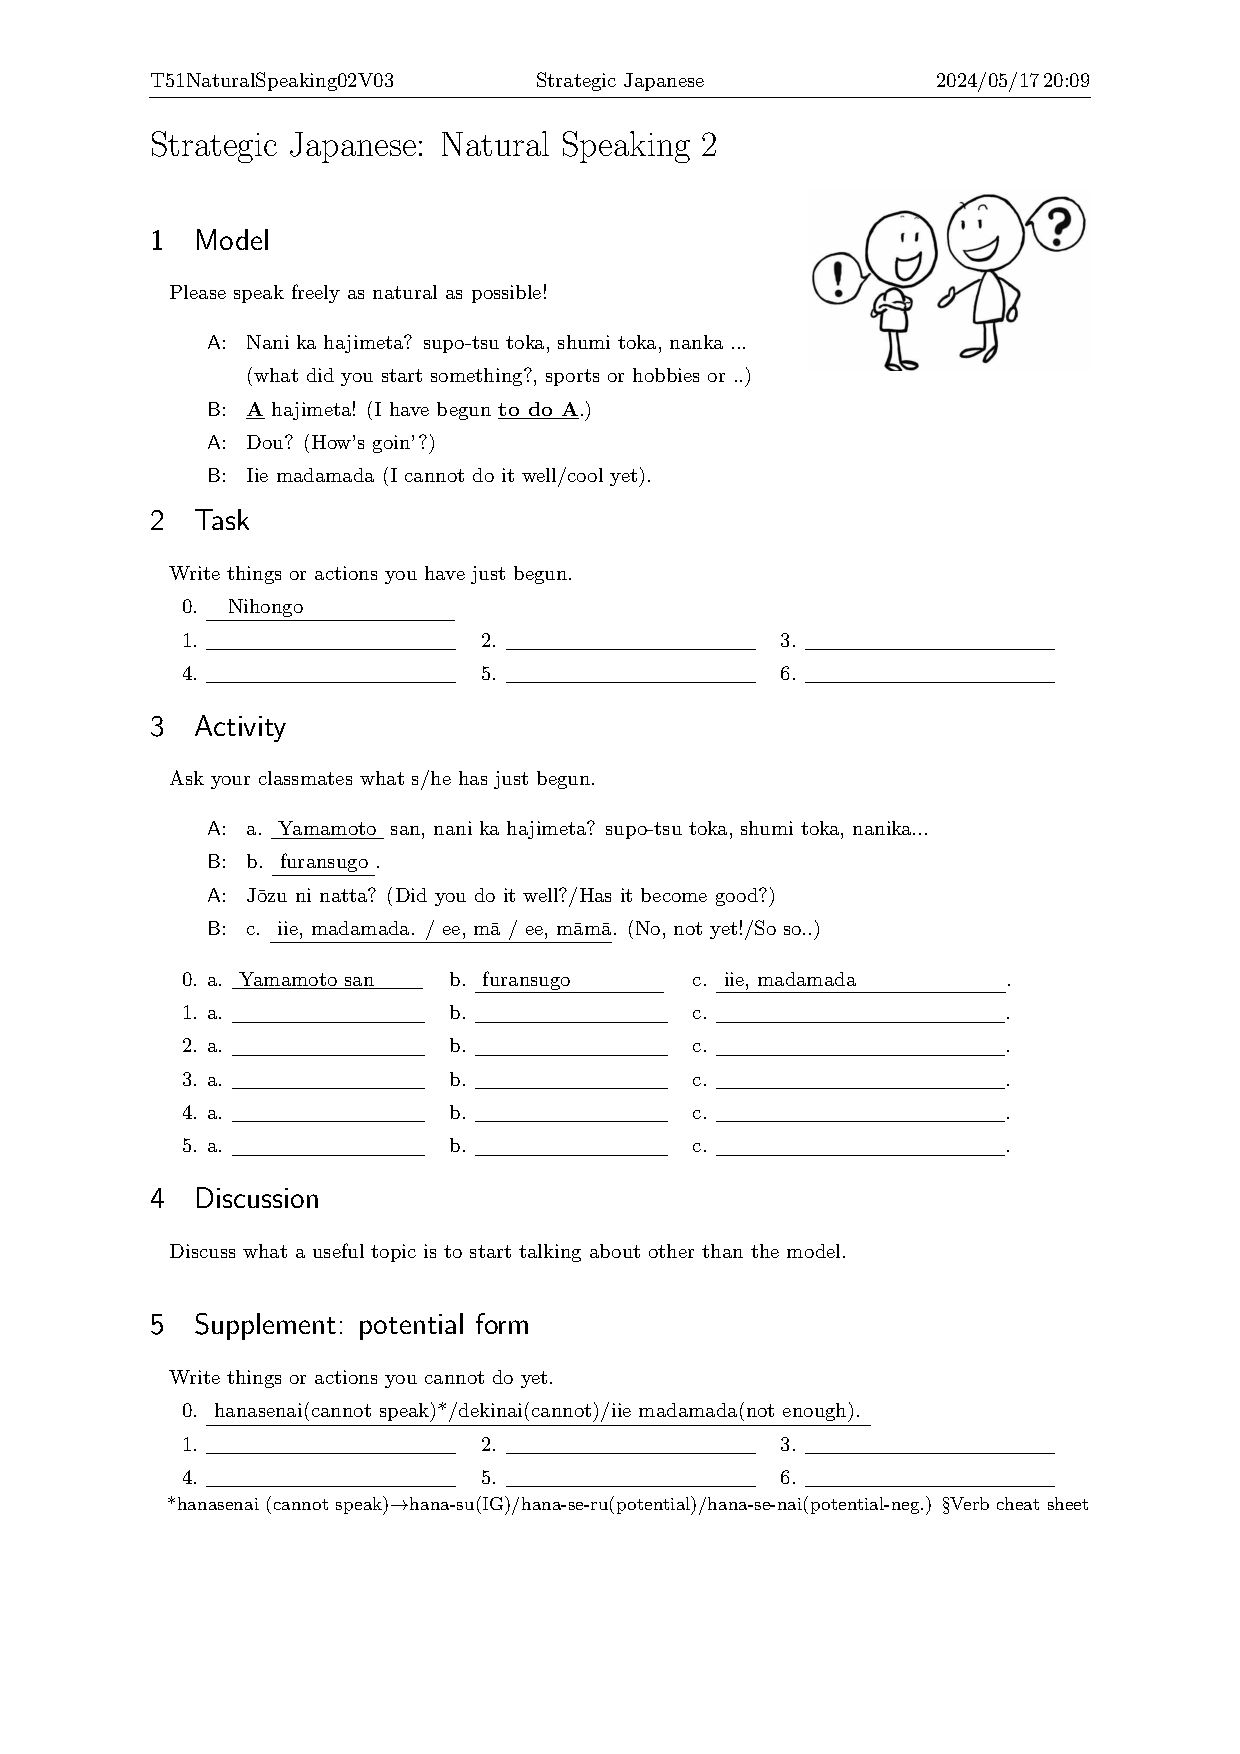
\includepdf[pages=-, scale=.86, trim=70 62 70 30, clip, offset=0mm -8.5mm, pagecommand={\thispagestyle{plain}}]{../T51NaturalSpeaking02V03.pdf}

\ifEnglish
\section{{\it Aru?\/}(Do you have it?)}
\else
  \section{「ある」は「持っている」の意味}
\fi

\ifEnglish
\subsection{Model}
\else
\subsection{モデル}
\fi
\begin{toiquestion}
\ifEnglish
Consider what {\bf aru\/} in the following model means.
\else
次のモデルにある「ある」はどんな意味であるかを考えなさい。
\fi
\end{toiquestion}

\begin{itemize}
 \item[A:] ima jikan {\bfseries aru}? (Do you have time now?)
 \item[B:] un. nani? (Yes, what?)
 \item[A:] pen {\bfseries aru}? (Do you have a pen?)
 \item[B:] aa, {\bfseries aruyo}. (Yap! I do!)
 \item[A:] ky\=o kurasu {\bfseries arimasu} ka? (Do you have a class today?)
 \item[B:] iie, {\bfseries arimasen}. (No, I don't)
\end{itemize}

\begin{note}
\ifEnglish
{\it arimasu\/}: polite expression of {\it aru\/} which is the continuative form of {\it aru\/} with the polite auxiliary verb {\it masu\/}. It is a formal expression.
\else
「あります」: 「ある」の連用形「あり」に丁寧の助動詞「ます」が付いた形。フォーマルな表現である。
\fi
\end{note}
\begin{note}
\ifEnglish
{\it arimasen\/}: the continuative form of {\it aru\/} with the negative form of the polite auxiliary verb {\it masu\/}. It is also a formal expression.
However, if you pronounce it strongly, it gives a cold impression, so it is better to reply just with {\it iie\/} (no).
\else
「ありません」: 「ある」の連用形「あり」に丁寧の助動詞「ます」の否定形「ません」が付いた形。
これもフォーマルな表現である。
しかし、強く発音すると冷たい印象を与えるので、「いいえ」とだけ、返答するのがよい。
\fi
\end{note}

\begin{toianswer}
\ifEnglish
In addition to the literal meaning of `to exist', {\it aru\/} also has the contextual meaning of `to have'.
In conversation, it is easier to ask {\it aru\/} than {\it motteiru\/}.
\else
「ある」は字義的な意味として「存在する」という意味以外に文脈的な意味として「持っている」という意味もある。
会話では「持っている?」と尋ねるよりも「ある?」と聞くほうが簡単である。
\fi%English
\end{toianswer}

\ifEnglish
\subsection{Activity}
\else
\subsection{アクティビティ}
\fi

\begin{toiquestion}
\ifEnglish
Ask your partner what they have and take notes.
\else
パートナーにどんなものを持っているかをいろいろ聞いて、メモを取りなさい。
\fi
\end{toiquestion}

\begin{itemize}
\item[A:] Suzuki san, \underline{keitai} aru? (Mr. Suzuki, do you have a mobile phone?)
\item[B:] un, aruyo./ uun, nai. (Yes, I do; No, I don't)
\end{itemize}

\setlength{\columnsep}{-10pt}
\begin{enumerate}
 \item[0.] \hrulefill\par
	   \vspace{-1.2\baselineskip}\hspace{.5em}{\bfseries Suzuki} san has {\bfseries a mobile phone, keitai}
	   \vspace{.2\baselineskip}
 \item \hrulefill
 \item \hrulefill
 \item \hrulefill
 \item \hrulefill
 \item \hrulefill
\end{enumerate}

\begin{toianswer}
\ifEnglish
Possessions are often relatively easy-to-remember words, simplified and short expressions, and proper nouns such as product names.
However, if you do not prepare in advance, it will not come out of your mouth immediately.
If you don't just memorize the words in your head, but actually speak through practice with a conversation partner, you will be able to remember them naturally even if you don't have much intention of memorizing them.
\else
所持品は比較的覚えやすい単語であるか、簡易化されて短かく表わさせたもの、商品名のような固有名詞などが多い。
しかし、あらかじめ準備しておかないとすぐに口から出てこない。
頭で覚えるだけでなく、実際に会話のパートナーと練習を通して発話すると覚えるつもりがあまりなくても自然に覚えられると思う。
\fi
\end{toianswer}

\ifEnglish
\subsection{Discussion}
\else
\subsection{ディスカッション}
\fi

\begin{toiquestion}
\ifEnglish
What kind of meaning do you think {\it aru\/} have?
\else
「ある」にはどんな意味があるか。
\fi
\end{toiquestion}
\begin{toianswer}
\ifEnglish
{\it Aru\/} basically means ``to exist,'' but it can also mean ``to possess.''
It is difficult to learn from textbooks how the basic meaning of a verb is used, so it is necessary to actually use the word to understand it.
The academic field that considers meaning such as this is called {\bf semantics\/}, and the academic field that considers usage is called {\bf pragmatics\/}.
\else
「ある」の基本的に「存在する」という意味があるが、そこから転じて、「所持する」という意味もある。
ある動詞の基本的な意味が、どのように使われるかを教科書で学ぶことは難しいので、実際にことばを使ってみて理解する必要がある。
このように意味を考える学問分野を意味論といい、使い方を考える学問分野を語用論という。
\fi
\end{toianswer}

\begin{toiquestion}
\ifEnglish
When and how can you use this expression?
\else
この表現は、いつ、どんなときに使えばよいか。
\fi
\end{toiquestion}
\begin{toianswer}
\ifEnglish
For example, when you want to borrow money or something you need, you can use it like {\it okane, aru?\/} (do you have money?);
when you want to talk to someone for a minute, you can use it like {\it nee, jikan, aru?\/} (do you have time?); and
when you are going to go out for something and you do some shopping for someone, you can use it like {\it nanika kaimono, aru?\/} (do you have something to buy?).
\else
たとえば、お金や必要なものを借りたいとき「お金、ある?」、
ちょっと誰かを話をしたいとき「ねぇ、ちょっと、時間、ある?」、
何かのついでに誰かのために買い物をしてきてあげようとするとき「買い物、ある?」のように使える。
\fi
\end{toianswer}



\ifEnglish
\section{{\it Shitteiru?\/}(Do you know?)/{\it shiranai\/}(I don't know)}
\else
\section{「知っている?」「知らない」}
\fi

\ifEnglish
People often ask questions in their daily lives.
\else
人が何かを尋ねる場面は日常生活では頻繁に見られることだろう。
\fi
\ifEnglish
When you ask someone if they know something, you can ask with {\it shitteiru?\/} (do you know?), but the negative form is {\it shiranai\/} (I don't know), not {\it shitteinai\/}.
Here, we will not learn how to use the suffix of progressive form,\,{\it -teiru\/}.
\else
人に何かを知っているかどうかを聞くときには「知っている?」と聞けばよいが、その否定形は「知らない」であって「知っていない」ではない。
ここでは、「~ている」の使い方は学ばない。
\fi
\ifEnglish
\subsection{Model}
\else
\subsection{モデル}
\fi

\begin{toiquestion}
\ifEnglish
Speak as naturally and freely as possible according to the following model.
\else
次のモデルにしたがって、できるだけ自然に自由に話しなさい。
\fi
\end{toiquestion}

\begin{itemize}
  \item[A:] \underline{Pikach\=u} {\bfseries shitte(i)ru}? (Do you know picach\=u?)
 \item[B:] Un, {\bfseries shitte(i)ru}. (Yes, I do)
 \item[A:] J\=a, \underline{Godzilla} wa? (How about Godzilla?)
 \item[B:] Uun, {\bfseries shiranai}. (No, I don't)
 \item[A:] Sensei, \underline{Godzilla} {\bfseries gozonji} desuka?\\(Professor! Do you know Godzilla?)
 \item[C:] Mochiron, {\bfseries shitte(i)masuyo}. (Of course, I do)
\end{itemize}

\begin{center}

\includegraphics[trim=5 17 100 10,clip,width=.20\hsize]{img/godzilla02.pdf}
\\\vspace*{0.2\baselineskip}
{\tiny Hilofumi Yamamoto}

\includegraphics[width=.08\hsize]{img/by-sa.png}
\vspace*{0\baselineskip}
\end{center}


\begin{note}
\ifEnglish
{\it shiru\/} (to know) $\rightarrow$ {\it shitteiru\/} (progressive: to know) /
{\it shiru\/} (dictionary form: to know) is not used in an ordinary situation;
the form of {\it -teiru\/} is used to indicate a continuing state.
If you pronounce it quickly, {\it i\/} will be omitted.
\else
知る $\rightarrow$ 知っている /
「知る」という形(辞書形)はあまり使われない。
続いている状態を表わす「~ている」の形が使われる。
早く発音すると「い」が省略される。% 2022-08-07
\fi
\end{note}

\begin{note} % 2022-08-06
\ifEnglish
{\it shiranai\/}: negative form of {\it shitteiru\/} (to know);
the form {\it shitteinai\/} is rarely used.
\else
知らない: 「知っている」の否定形。「知っていない」の形はあまり使われない。
\fi
\end{note}

\begin{note}
\ifEnglish
{\it gozonji\/}: honorific form of {\it shitteiru\/} (to know)
\else
ごぞんじ: 「知っている」の尊敬形
\fi
\end{note}

\begin{toianswer}
\ifEnglish
The verb {\it shiru\/} is often used in conversation in the form of {\it shitteiru\/}.
However, its negative form is not {\it shitteinai\/} but {\it shiranai\/}.
Many students make the mistake of answering {\it shitteinai\/}.
In addition, {\it gosonji\/} is an honorific expression for {\it shitteiru\/}, but there is no equivalent form for {\it -teiru\/}.
\else
「知る」という動詞は、会話では多く「知っている」の形で使われる。
しかし、その否定形は「知っていない」ではなく「知らない」の形で使われる。
多くの学生が「知っていない」と答えて間違える。
また、「ごぞんじ」は「知っている」の敬語表現だが、「〜ている」に相当する形はない。
\fi%English

\ifEnglish
Have a conversation using the proper nouns of singers and actors you know, celebrities in your country, famous artists, and athletes.
\else
自分の知っている歌手や俳優、自分の国の有名人、有名な芸術家、スポーツ選手などの固有名詞を使って、会話をしてみよう。
\fi
\ifEnglish
Be careful not to say {\it shitteinai\/} when answering in the negative.
\else
否定形で答えるときに、「知っていない」と言わないように注意すること。
\fi
\end{toianswer}


\ifEnglish
\subsection{Task}
\else
\subsection{タスク}
\fi

\begin{toiquestion}
\ifEnglish
Think of words that could be used for the underlined parts of the model above and make a note of them.
\else
上のモデルのアンダーラインの部分に使えそうな語を考えてメモしなさい。
\fi
\end{toiquestion}
\begin{toianswer}
\ifEnglish
It can be a manga or anime title or a character.
It is a good idea to prepare various proper nouns such as the names of world-famous artists, actors, singers, tourist spots, cities, etc. and you have a conversation with them.
\else
マンガやアニメのタイトルでもキャラクターでもよい。
世界的に有名な芸術家、俳優、歌手の名前、観光地、都市など、さまざまな固有名詞をあらかじめ準備しておいて、会話をしてみるとよい。
\fi
\end{toianswer}


\ifEnglish
\subsection{Activity}
\else
\subsection{アクティビティ}
\fi

\begin{toiquestion}
\ifEnglish
Ask your partners if they know something, and take notes.
\else
何か知っていそうなものを相手に質問して、メモをとりなさい。
\fi
\end{toiquestion}

\begin{enumerate}
 \item[0.] \hrulefill\par
	   \vspace{-1.2\baselineskip}\hspace{.5em}I asked {\bfseries Suzuki} san if he knows {\bfseries Godzilla } or not: iie, {\bfseries shiranai}/ hai, {\bfseries shitteiru}

 	   \vspace{.2\baselineskip}

 \item \hrulefill
 \item \hrulefill
 \item \hrulefill
 \item \hrulefill
 \item \hrulefill
\end{enumerate}

\begin{toianswer}
\ifEnglish
You can write your notes in either Japanese or English.
Listen carefully to what nouns your conversation partner uses.
People's names and proper nouns are difficult to hear.
If you do not actually know the person or noun, you'll find it difficult to hear.
You can use English, so ask what the person or noun is.
\else
ノートは日本語でも英語でもどちらで書いてもかまわない。
会話の相手がどんな名詞を使ったかをよく聞いてください。
人の名前や固有名詞は聞き取るのが難しい。
実際にその人物や名詞を知らなければ、聞き取るのが難しいことがわかるはずだ。
英語を使ってもよいので、その人物や名詞がどういうものなのかを尋ねてみよう。
\fi
\end{toianswer}


%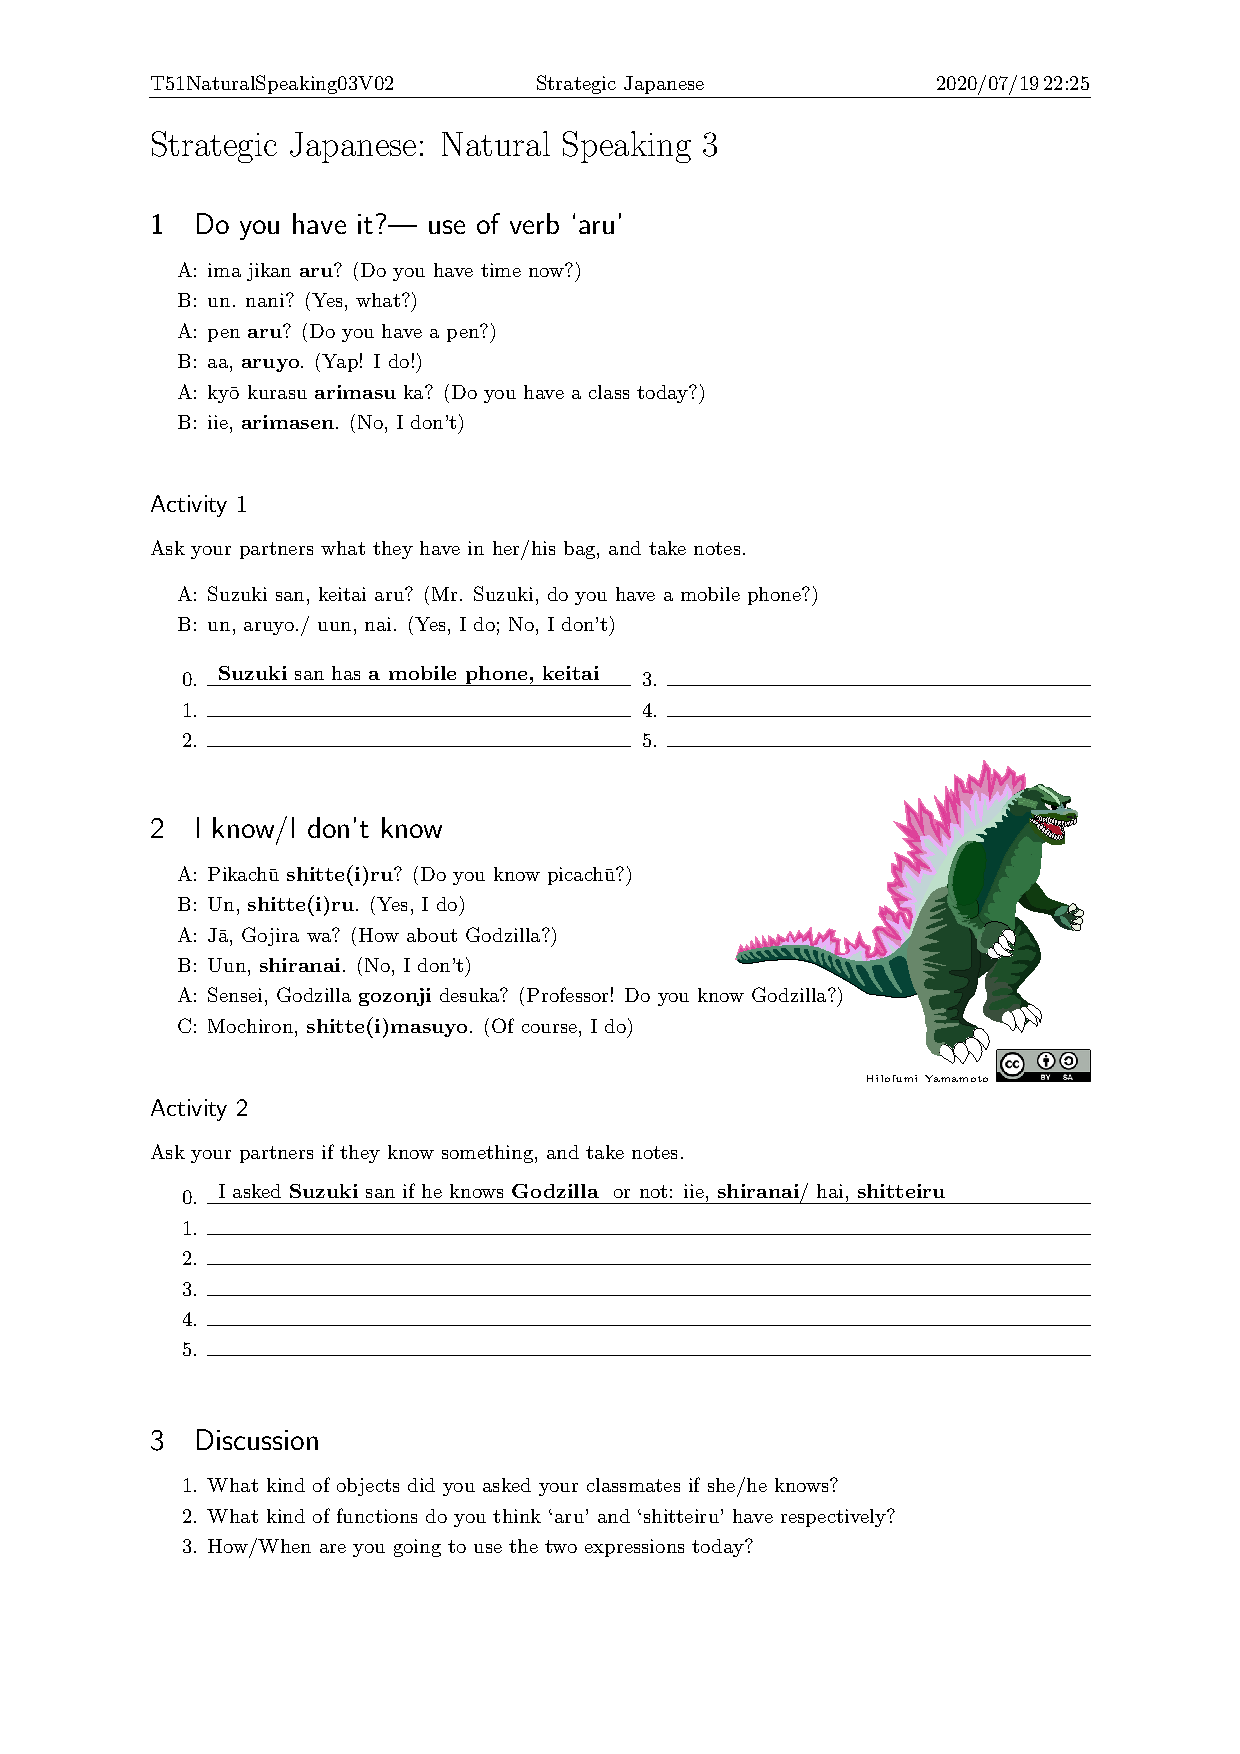
\includepdf[pages=-, scale=.86, trim=70 62 70 30, clip, offset=0mm -8.5mm, pagecommand={\thispagestyle{plain}}]{../T51NaturalSpeaking03V02.pdf}

\ifEnglish
  \section{Telling an opinion/impression/feeling}
\else
  \section{感想・印象・感情を話す}
\fi

%Natural Speaking 4 (File: T51NaturalSpeaking04V02)
\ifEnglish
Learn formal style, casual style, male and female language, feelings and monologues.
\else
フォーマル・スタイル、カジュアル・スタイル、男性言葉、女性言葉、感情や独り言を学ぶ。
\fi

\ifEnglish
\subsection{Model}
\else
\subsection{モデル}
\fi

\begin{toiquestion}
\ifEnglish
Read casual style and formal style separately and discuss how they differ.
Discuss how male and female words make you feel.
\else
カジュアル・スタイルとフォーマル・スタイルをそれぞれ読み、どんな違いがあるか、話し合いなさい。
男ことばと女ことばはそれぞれどんな感じがするか、意見を交換しなさい。
\fi
\end{toiquestion}

\begin{description}
\item Casual: (yokatta/umi ni/itta)
\begin{description}
 \item[A:] Aa \underline{{\bfseries yokatta}}! (That was good!)
 \item[B:] Nani ga? (What was good?)
 \item[A:] \underline{{\bfseries Umi ni itta}} n da (male)/no (female).
 \item[B:] Sou! \underline{{\bfseries sore wa ii}} ne. (Really! It sounds good)
\end{description}

\vspace{1\baselineskip}

\item Formal: (yokatta/umi ni/itta n desu)
\begin{description}
 \item[A:] Aa \underline{{\bfseries yokatta}}! (That was good!)
 \item[B:] Nani ga desuka? (What was good?)
 \item[A:] \underline{{\bfseries Umi ni itta}} n desu.(I went to sea.)
 \item[B:] Soudesuka! \underline{{\bfseries sore wa ii}} desune. (Really! It sounds good)
\end{description}
\end{description}

\begin{figure}[h]
  \begin{center}
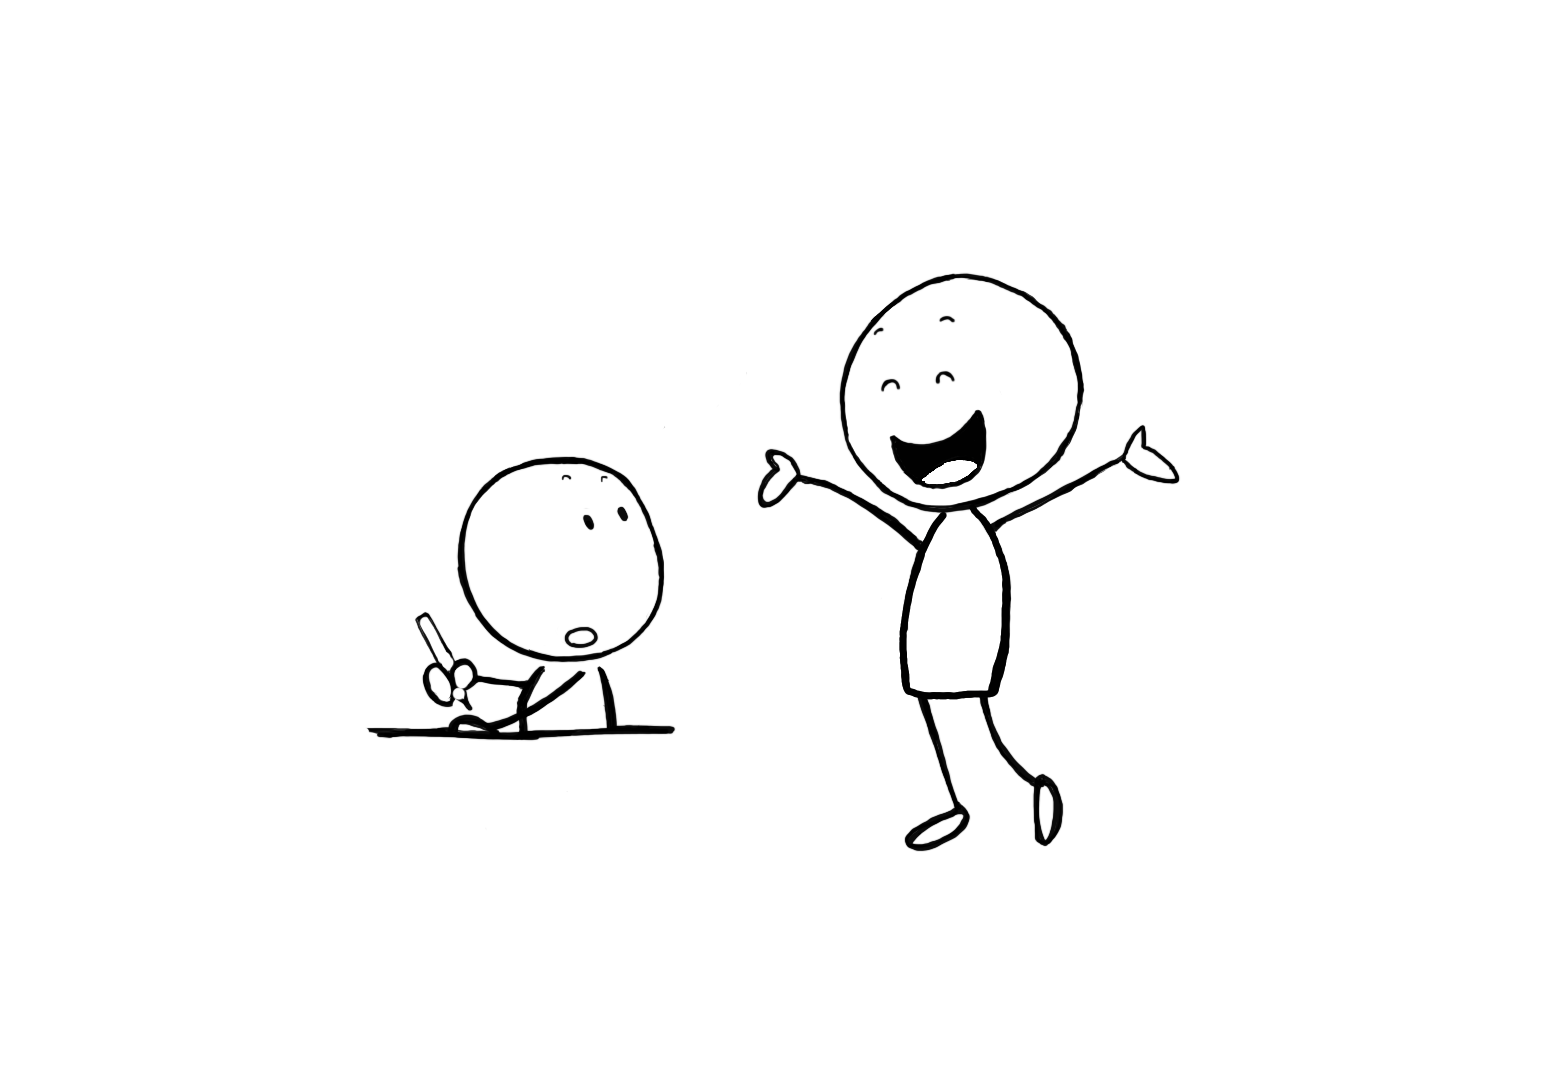
\includegraphics[trim=200 130 200 150, clip, width=.3\hsize]{img/T51NaturalSpeech04image.png}
  \end{center}
  \ifEnglish
  \caption{Aa yokatta!/It was good!}
  \else
  \caption{ああ、よかった!}
  \fi
  \label{fig:aayokatta}
\end{figure}



\ifEnglish
\subsection{Task}
\else
\subsection{タスク}
\fi

\begin{toiquestion}
\ifEnglish
Write i-adjectives in past tense and polite form.
\else
イ形容詞を過去形と丁寧語で書く。
\fi
\end{toiquestion}

\begin{enumerate}
\item[0.]
  \underline{\hspace{1em}ii/yoi\hspace{1em}$\rightarrow$\hspace{2em}yokatta\hspace{1em}$\rightarrow$\hspace{2em}yokatta desune\hspace{2.7em}}
\item \underline{\hspace{24em}} \rule{0mm}{3.5mm}
\item \underline{\hspace{24em}}
\item \underline{\hspace{24em}}
\item \underline{\hspace{24em}}
\item \underline{\hspace{24em}}
\end{enumerate}

\begin{toianswer}
\ifEnglish
To form the past tense of i-adjectives, remove the {\it i\/} at the end of the word and add {\it katta\/}.
However, in the case of {\it ii\/} (good), {\it yoi\/} is used instead of {\it ii\/} and {\it i\/} of {\it yoi\/} is replaced with {\it katta\/}.
There are some textbooks where {\it desu\/} is used as a polite form of i-adjectives, such as {\it iidesu\/} and {\it yokatta desu\/}, but some people find it a little childish, so it's better to avoid to use it.
If you really want to use an expression with {\it desu\/}, it will be natural to add a final particle such as {\it iidesu yo\/} or {\it yokatta desu yo\/}.
However, we have to decide whether to add {\it ne\/} or {\it yo\/}, and it is troublesome to add something when there is no need to attach anything.
\else
イ形容詞の過去形の作り方は、語尾の「い」を取り除いて、「かった」を付ける。
ただし、「いい」の場合は「いい」ではなく「よい」の「い」を取り除いて、「かった」を付ける。
イ形容詞の丁寧形として「いいです」「よかったです」のように「です」をそのまま付ける教科書も見られるが、少し幼稚と感じる人もいるので、避けた方がよい。
どうしても「です」を付けた表現を使いたい場合には、「いいですよ」「いいですね」「よかったですね」のように終助詞を付けると自然になる。
しかし、「ね」を付けるか、「よ」を付けるかを考えなければならないし、もともと何も付けなくてもよいときに、何かを付けることは面倒である。
\fi
\end{toianswer}

%\ifEnglish
%\subsection{Task B}
%\else
%\subsection{タスクB}
%\fi

\begin{toiquestion}
\ifEnglish
Write down what you want to tell, experiences, events you want to mention, such as good things and happy things.
\else
「よかったこと」「うれしかったこと」など、自分が伝えたいこと、経験、言及したいイベントを書きなさい。
\fi
\end{toiquestion}

\begin{enumerate}
  \item[0.] \underline{\hspace{1em}umi ni itta\hspace{18.2em}}
  \item \underline{\hspace{24em}}
  \item \underline{\hspace{24em}}
  \item \underline{\hspace{24em}}
  \item \underline{\hspace{24em}}
  \item \underline{\hspace{24em}}
\end{enumerate}

\begin{note}
\ifEnglish
When referring to a past event with a verb, use the past tense of the verb.
The formation of the past tense of verbs is the same as the formation of the te-form of verbs, except that ``te'' is replaced with ``ta.''
$\rightarrow$  \S\,\ref{te-form}, Table\,\ref{tab:teform}
\else
過去の出来事を動詞で言うときは、動詞の時制を過去にします。
動詞の過去形の作り方は、「て」を「た」に置き換える点以外は動詞のテ形の作り方と同じである。
$\rightarrow$ \S\,\ref{te-form}, Table\,\ref{tab:teform}
\fi
\end{note}

\begin{toianswer}
\ifEnglish
It can be an event such as {\it ryoko ni itta\/} (going on a trip), {\it karaoke ni itta\/} (going to karaoke), {\it dizuniirando ni itta\/} (going to Disneyland), or {\it Okinawa ni itta\/} (going to Okinawa: Southern islands in Japan), or it can be something you do in your daily life, such as {\it resutoran ni tomodachi to itta\/} (going to a restaurant with friends) or {\it kaimono ni itta\/} (going shopping).
\else
旅行に行った、カラオケに行った、ディズニーランドに行った、沖縄に行った、などイベントでもよいし、友達とレストランに行った、買い物に行ったのような日常生活で行なうことでもよい。
\fi
\end{toianswer}

\ifEnglish
\subsection{Activity}
\else
\subsection{アクティビティ}
\fi

\begin{toiquestion}
\ifEnglish
Ask your classmates in both casual style and formal style.
\else
カジュアルなスタイルとフォーマルなスタイルの両方で、クラスメートに聞いてみよ。
\fi
\end{toiquestion}

\begin{quote}
\begin{description}
 \item[A:] a. Aa, \underline{\hspace{1em}}\,yokatta.\hspace{-3.2em}\underline{\hspace{5em}}
 \item[B:] b. \underline{ Suzuki } san, nani ga \underline{\hspace{1em}}\,yokatta\hspace{-2.9em}\underline{\hspace{4em}} no?
 \item[A:] c. \underline{{\bfseries Umi ni itta}} n desu.
 \item[B:] Sou, sore wa ii ne.
\end{description}
\end{quote}

\begin{tabular}[t]{lll}
 0. a. \underline{ Yokatta \hspace{3.5zw}}
 &  b. \underline{ Suzuki\hspace{4.8zw}}
 &  c. \underline{ umi ni itta\hspace{4.5zw}}.\\
 1. a. \underline{\hspace{8zw}}& b. \underline{\hspace{8zw}} & c. \underline{\hspace{10zw}}.\\
 2. a. \underline{\hspace{8zw}}& b. \underline{\hspace{8zw}} & c. \underline{\hspace{10zw}}.\\
 3. a. \underline{\hspace{8zw}}& b. \underline{\hspace{8zw}} & c. \underline{\hspace{10zw}}.\\
 4. a. \underline{\hspace{8zw}}& b. \underline{\hspace{8zw}} & c. \underline{\hspace{10zw}}.\\
 5. a. \underline{\hspace{8zw}}& b. \underline{\hspace{8zw}} & c. \underline{\hspace{10zw}}.\\
\end{tabular}

\begin{toianswer}
\ifEnglish
In addition to {\it yokatta\/} (it was good), you can also use {\it omoshirokatta\/} (it was interesting), {\it tanoshikatta\/} (it was fun), {\it muzukashikatta\/} (it was difficult), {\it oishikatta\/} (it was delicious), {\it bikkurishita\/} (it was surprised).
\else
「よかった」以外に、「おもしろかった」「楽しかった」「難しかった」「おいしかった」「びっくりした」など使えるだろう。
\fi
\end{toianswer}


\ifEnglish
\subsection{Discussion}
\else
\subsection{ディスカッション}
\fi

\begin{toiquestion}
\ifEnglish
How did you feel when you were speaking naturally?
\else
自然に話していた時の気持ちはどうか。
\fi
\end{toiquestion}
\begin{toianswer}
\ifEnglish
Even though you didn't know what kind of response the other party would give you, you could have talked more relaxedly than before.
\else
相手からどんな返答が返ってくるかわからないのに、多少、以前よりリラックスして話せただろう。
\fi
\end{toianswer}

\begin{toiquestion}
\ifEnglish
What is the point of how to speak naturally?
\else
自然な話し方のポイントは?
\fi
\end{toiquestion}
\begin{toianswer}
\ifEnglish
Little by little, perhaps, you've come to realize that what you say matters more than the form of language.
You're starting to feel that the language form isn't difficult if you keep it short.
\else
少しずつかもしれないが、言語の形よりも話している内容の方が重要だということに気づいてきただろう。
言語の形式は短かく話せば、難しくないと感じ始めているだろう。
\fi
\end{toianswer}

\begin{toiquestion}
\ifEnglish
What kind of techniques or words can you add to improve your speech?
\else
スピーチを上達させるには、どんなテクニックや表現を加えればよいか。
\fi
\end{toiquestion}
\begin{toianswer}
\ifEnglish
In our daily lives, we often express ``feelings/impressions/impressions'' such as ``Oh, that was good'' and ``Oh, I'm happy.''
It's a good idea to find a way to express your feelings directly to someone on the Internet, learn it yourself, and use it.
\else
「ああ、よかった」「ああ、うれしい」などのように「感情・印象・感想」を発話することは生活の中で多い。
誰かに気持ちを直接伝える言い方をインターネットで見つけて自分で覚えて使ってみるのは良いことである。
\fi%English
\end{toianswer}

%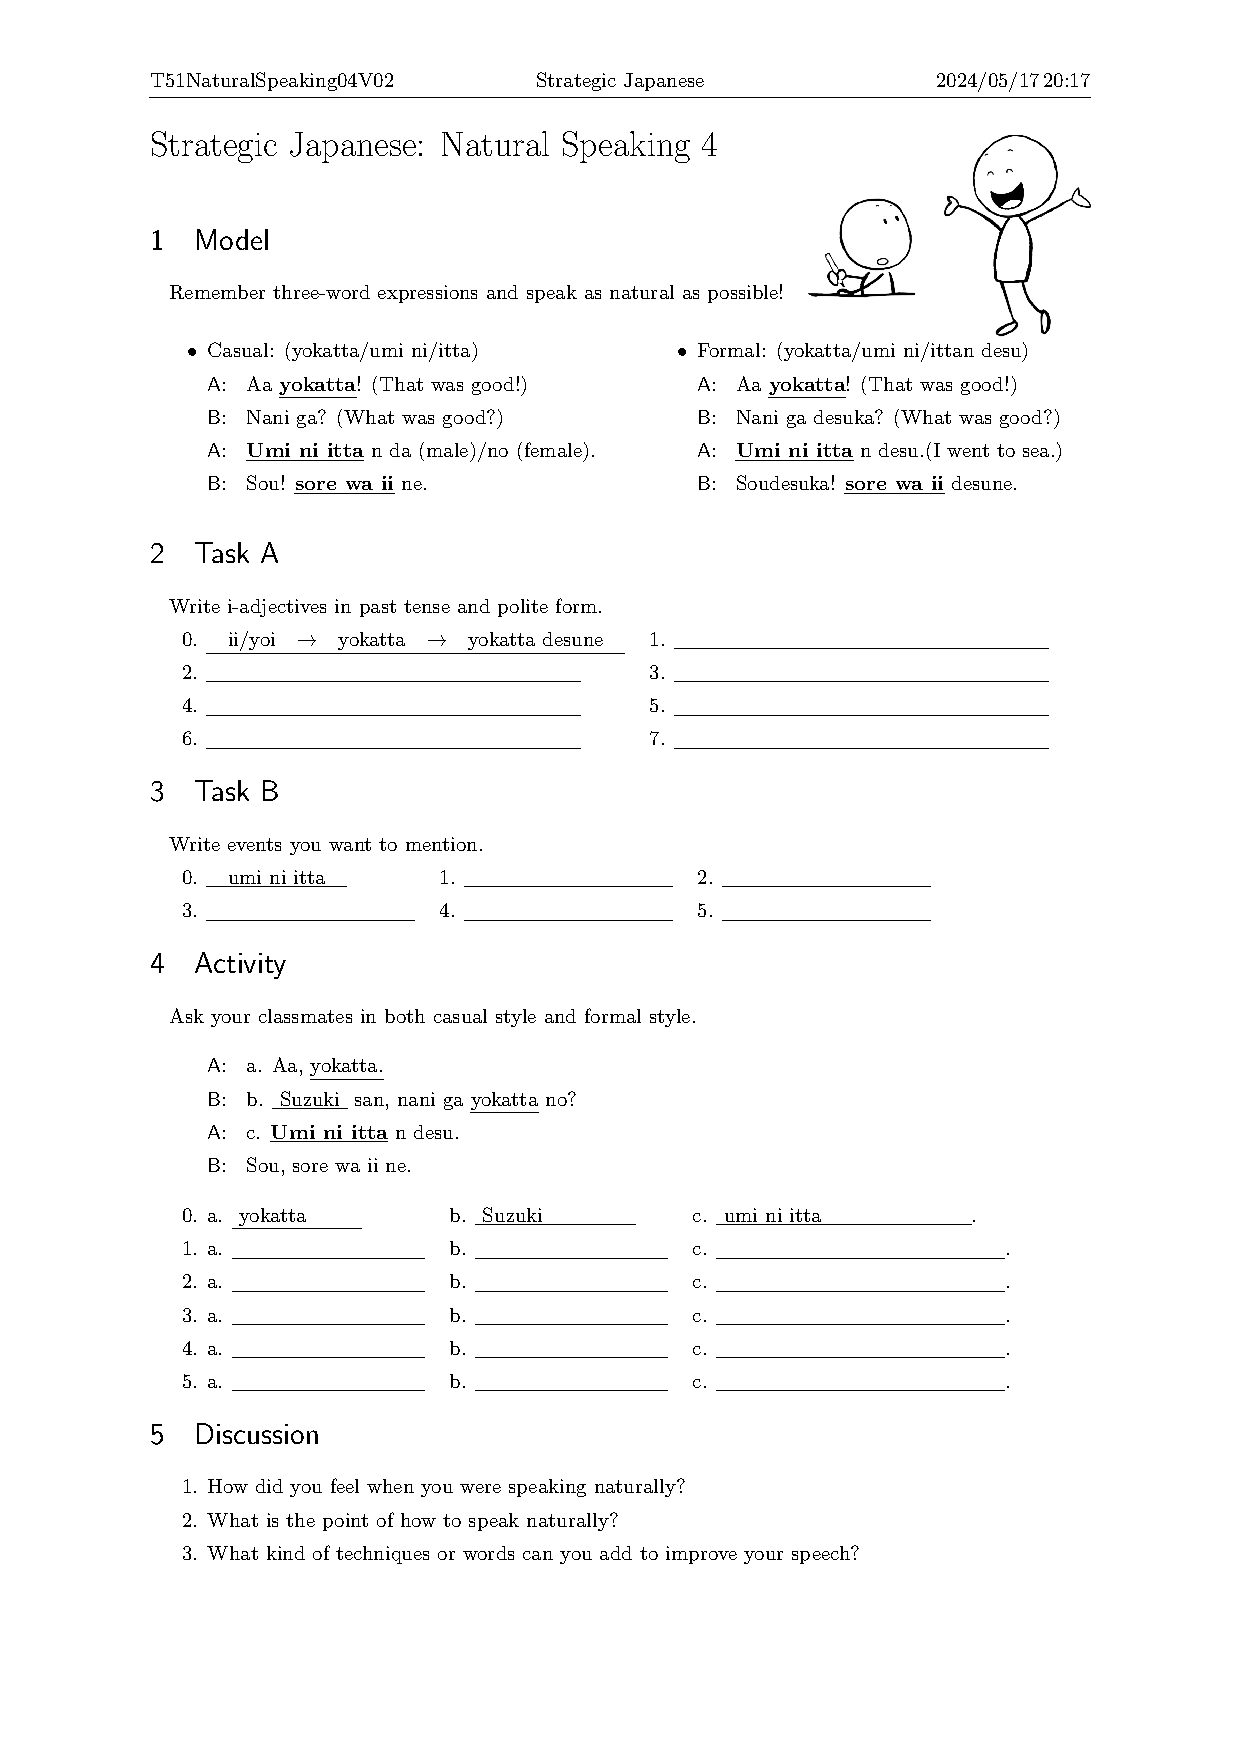
\includepdf[pages=-, scale=.86, trim=70 62 70 30, clip, offset=0mm -8.5mm, pagecommand={\thispagestyle{plain}}]{T51NaturalSpeaking04V02.pdf}

\fi%NATURALSPEAKINGPARTONE

\ifNATURALSPEAKINGPARTTWO
\ifEnglish
\chapter{Natural Speaking: Part 2}
\else
\chapter{自然に話すこと: Part 2}
\fi

\begin{abstract}
\ifEnglish
You will learn casual and formal style of conversations;
\else
カジュアルとフォーマルスタイル。
\fi
\ifEnglish
{\it mada\/} (not yet) and {\it mou\/} (have already done);
\else
「まだ」と「もう」
\fi
\ifEnglish
verb conjugation, past/perfect form;
\else
日本語の助動詞「た」は過去を示すだけでなく、完了も示せる。
否定は「まだ〜ていない」ではあるが、実際には「〜ない」と言っても良い。
\fi
\ifEnglish
invitation and response; and
\else
誘いと反応、
\fi
\ifEnglish
learn expressions to ask what your conversation person is doing on the phone or by e-mail.
\else
電話やメールなどで相手が今何をしているかを聞く表現を学ぶ。
\fi
\end{abstract}


\ifEnglish
\section{Yet, already, and verb past/perfect}
\else
\section{もう・まだ・過去形・完了形}
\fi

%Natural Speaking 5 (File: T51NaturalSpeaking05V02)

\ifEnglish
{\it Mada\/} (not yet) and {\it mou\/} (have already done);
\else
「まだ」と「もう」
\fi
\ifEnglish
Verb conjugation, past/perfect form;
Japanese auxiliary verb {\it ta\/} not only indicates the past, but also the completion;
negation is {\it mada ... teinai\/} (not yet), but it is possible to say {\it ..nai\/} (not) in fact.
\else
日本語の助動詞「た」は過去を示すだけでなく、完了も示せる。
否定は「まだ〜ていない」ではあるが、実際には「〜ない」と言っても良い。
\fi

\ifEnglish
\subsection{Model}
\else
\subsection{モデル}
\fi

\begin{toiquestion}
\ifEnglish
Please speak freely as natural as possible.
Prepare the following three words {\it nee, mou tabeta?\/}.
\else
なるべく自然に、自由に話す。
次の3語以内の表現を使う。「ねぇ、もう、食べた」
\fi
\end{toiquestion}

\begin{description}
\item Casual:
\begin{description}
 \item[A:] Nee, \underline{{\bfseries mou tabeta}}? (Have you already eaten?)
 \item[B:] \underline{{\bfseries Un, tabeta.}} (Yes, I have) /\underline{{\bfseries Uun, mada.}} (No, I haven't yet)
 \item[A:] Nee, mou \underline{{\bfseries itta}}? (Have you already been there?)
 \item[B:] \underline{{\bfseries Un, itta.}} (Yes, I have) /\underline{{\bfseries Uun, mada.}} (No, I haven't)
\end{description}
\item Formal:
\begin{description}
 \item[A:] Suzuki san, \underline{{\bfseries m\=o  tabemashita}}?
 \item[B:] \underline{{\bfseries Ee, tabemashita.}} /\underline{{\bfseries Iie, mada.}}
 \item[A:] Nee, mou \underline{{\bfseries ikimashita}}?
 \item[B:] \underline{{\bfseries Ee, ikimashita.}} /\underline{{\bfseries Iie, mada.}}
\end{description}
\end{description}

\ifEnglish
\subsection{Task}
\else
\subsection{タスク}
\fi

\begin{toiquestion}
\ifEnglish
Convert the following verbs into past tense and past formal style.
\else
動詞を過去形に変換し、過去形のフォーマルなスタイルにしなさい。
\fi
\end{toiquestion}

\begin{enumerate}
  \item[0.] {\bfseries taberu (eat) $\rightarrow$ tabeta $\rightarrow$ tabemasu $\rightarrow$ tabemashita}\hrulefill
  \item miru (see)    $\rightarrow$ \hrulefill
  \item yomu (read)   $\rightarrow$ \hrulefill
  \item kaku (write)  $\rightarrow$ \hrulefill
  \item tsukuru (make)$\rightarrow$ \hrulefill
  \item iku  (go)     $\rightarrow$ \hrulefill
  \item suru (do)     $\rightarrow$ \hrulefill
  \item kuru (come)   $\rightarrow$ \hrulefill
\end{enumerate}

\begin{toianswer} % 2022-08-16
\ifEnglish
Since {\it miru\/} (see) is a verb in the II group, it becomes {\it mita, mimashita\/}.
Since {\it yomu\/} (read), {\it kaku\/} (write), and {\it tsukuru\/} (make) are also verbs in the I group, they become {\it yonda, yomimashita\/}, {\it kaita, kakimashita\/}, and {\it tsukutta, tsukurimashita\/} respectively.
When a verb ends in {\it ru\/}, it has two possibilities, I group and II group, so be careful.
In that case, you first check if the nai(negation)-form of the verb includes A-row, neither I nor E-row.
We will find that {\it tsukuru\/} is in the I group since its nai-form is {\it tsukur-a-nai\/}.
Since the dictionary form of {\it iku\/}(go) ends with {\it ku\/}, {\it iku\/}, if you exactly follow the rules, it should be {\it iita\/}, but it conjugates irregulary {\it itta\/}, and its polite past form is {\it ikimashita\/}.
Since {\it suru\/}(do) is a group III verb, it becomes {\it shita, shimashita\/}.
Since {\it kuru\/}(come) is also a group III verb, it becomes {\it kita, kimashita\/}.
$\rightarrow$ \S\,\ref{te-form}, Table\,\ref{tab:teform}
\else
「見る」はIIグループの動詞なので、「見た、見ました」。
「読む」はIグループの「む」が辞書形の動詞なので、「読んだ、読みました」。
「書く」はIグループの「く」が辞書形の動詞なので、「書いた、書きました」。
「作る」はIグループの「る」が辞書形の動詞なので、「作った、作りました」。
ただし、「る」で終わる動詞はIIグループにもあるので、未然形が「あ行」になるかどうかを確かめる必要がある。
「作る」は未然形が「作らない」なので、Iグループであることがわかる。
「行く」はIグループの「く」が辞書形の動詞なので、ルール通りならば、「行いた」となるはずであるが、「いいた」は「いた」と区別しにくいので、例外的に「行った」になり、「行った、行きました」。
「する」はIIIグループの動詞なので、「した、しました」。
「来る」はIIIグループの動詞なので、「来た、来ました」。
$\rightarrow$ \S\,\ref{te-form}, Table\,\ref{tab:teform}
\fi
\end{toianswer}


\ifEnglish
\subsection{Activity}
\else
\subsection{アクティビティ}
\fi

\begin{toiquestion}
\ifEnglish
Ask your classmates in both casual and formal style.
\else
カジュアルなスタイルとフォーマルなスタイルの両方で、クラスメートに聞いてみなさい。
\fi
\end{toiquestion}

\begin{description}
 \item Casual:
\begin{description}
 \item[A:]  \underline{ Suzuki } san, mou \underline{tabeta}?
 \item[B:] \underline{ Un, mou tabeta.}/\underline{ Uun, mada.}
\end{description}
 \item Formal:
\begin{description}
 \item[A:] \underline{ Tanaka } sensei, mou \underline{tabemashitaka}?
 \item[C:] \underline{ Ee, mou tabemashitayo.}/\underline{ Iie, mada desuyo.}
\end{description}
\end{description}

\begin{enumerate}
  \item[0.] a.\underline{ Suzuki\hspace{6.4zw}} b.\underline{ tabeta\hspace{6.64zw}} c.\underline{ mou or mada \hspace{3.5zw}}.
  \item a.\underline{\hspace{10zw}}  b.\underline{\hspace{10zw}}  c.\underline{\hspace{10zw}}.
  \item a.\underline{\hspace{10zw}}  b.\underline{\hspace{10zw}}  c.\underline{\hspace{10zw}}.
  \item a.\underline{\hspace{10zw}}  b.\underline{\hspace{10zw}}  c.\underline{\hspace{10zw}}.
  \item a.\underline{\hspace{10zw}}  b.\underline{\hspace{10zw}}  c.\underline{\hspace{10zw}}.
  \item a.\underline{\hspace{10zw}}  b.\underline{\hspace{10zw}}  c.\underline{\hspace{10zw}}.
\end{enumerate}

\begin{toianswer}
\ifEnglish
For situations where {\it mou\/} and {\it mada\/} are used, it is good to think of situations where you have to say completed or incomplete, such as {\it gohan, dekita?\/} (is the meal ready?) or {\it shukudai, owatta?\/} (have you done your homework?).
\else
「もう」「まだ」が使う場面には、「御飯ができた」「宿題が終った」のような完了、未完了を言わなければならない場面を考えるとよい。
\fi
\end{toianswer}

\ifEnglish
\subsection{Discussion}
\else
\subsection{ディスカッション}
\fi

\begin{toiquestion}
\ifEnglish
How do you feel that you speak a way as short as possible?
\else
なるべく短い方法で話すというのはどうだったか?
\fi
\end{toiquestion}
\begin{toianswer}
\ifEnglish
In order to speak in short sentences, it is necessary to choose the most important words.
Saying more than the necessary information forces the listener to hear more than the expected words.
Speaking only the most important words makes it easier for your conversation partner to understand.
Also, if you make a mistake, you can easily correct it.
\else
短かい文で話すためには、もっとも重要な語を選ぶ必要がある。
必要な情報以外を言うと、聞き手は予測していた語以外も聞かなければならない。
もっとも重要な語だけを話すと、会話の相手にとっても理解しやすくなる。
また、言い間違えたときも、言い直しが簡単である。
\fi
\end{toianswer}

\begin{toiquestion}
\ifEnglish
What is the point of how to speak naturally?
\else
自然な話し方のポイントは?
\fi
\end{toiquestion}
\begin{toianswer}
\ifEnglish
Say briefly what your conversation partner need and expects.
If you have to think for a moment, don't be silent, say {\it eetoo\/} or {\it anoo\/} to show that you are willing to talk.
\else
必要な内容、相手の期待する内容をできるだけ短かく言うこと。
もし、瞬間的に考えなければならないときは、黙っていないで、「えーっと」「あのー」などを発話して、話す意思があることを示すこと。
\fi
\end{toianswer}

\begin{toiquestion}
\ifEnglish
What kind of techniques or words do you want to add to improve your speaking style?
\else
自分の話し方を改善するために、どのようなテクニックや単語を加えたいか?
\fi
\end{toiquestion}
\begin{toianswer}
\ifEnglish
Think of some situations where {\it mou\/} and {\it mada\/} are necessary.
Think about situations in your own language where you would use the words {\it mou\/} and {\it mada\/}.
If you don't know what you are being asked, it's a good idea to answer {\it e? nani?\/}.
\else
「もう」「まだ」が必要な場面を考える。自分の言語で「もう」「まだ」を使う場面を考えてみる。
何を尋ねられたかわからないときは、とりあえず、「えっ?何ですか?」と答えておくのもよい。
\fi
\end{toianswer}

%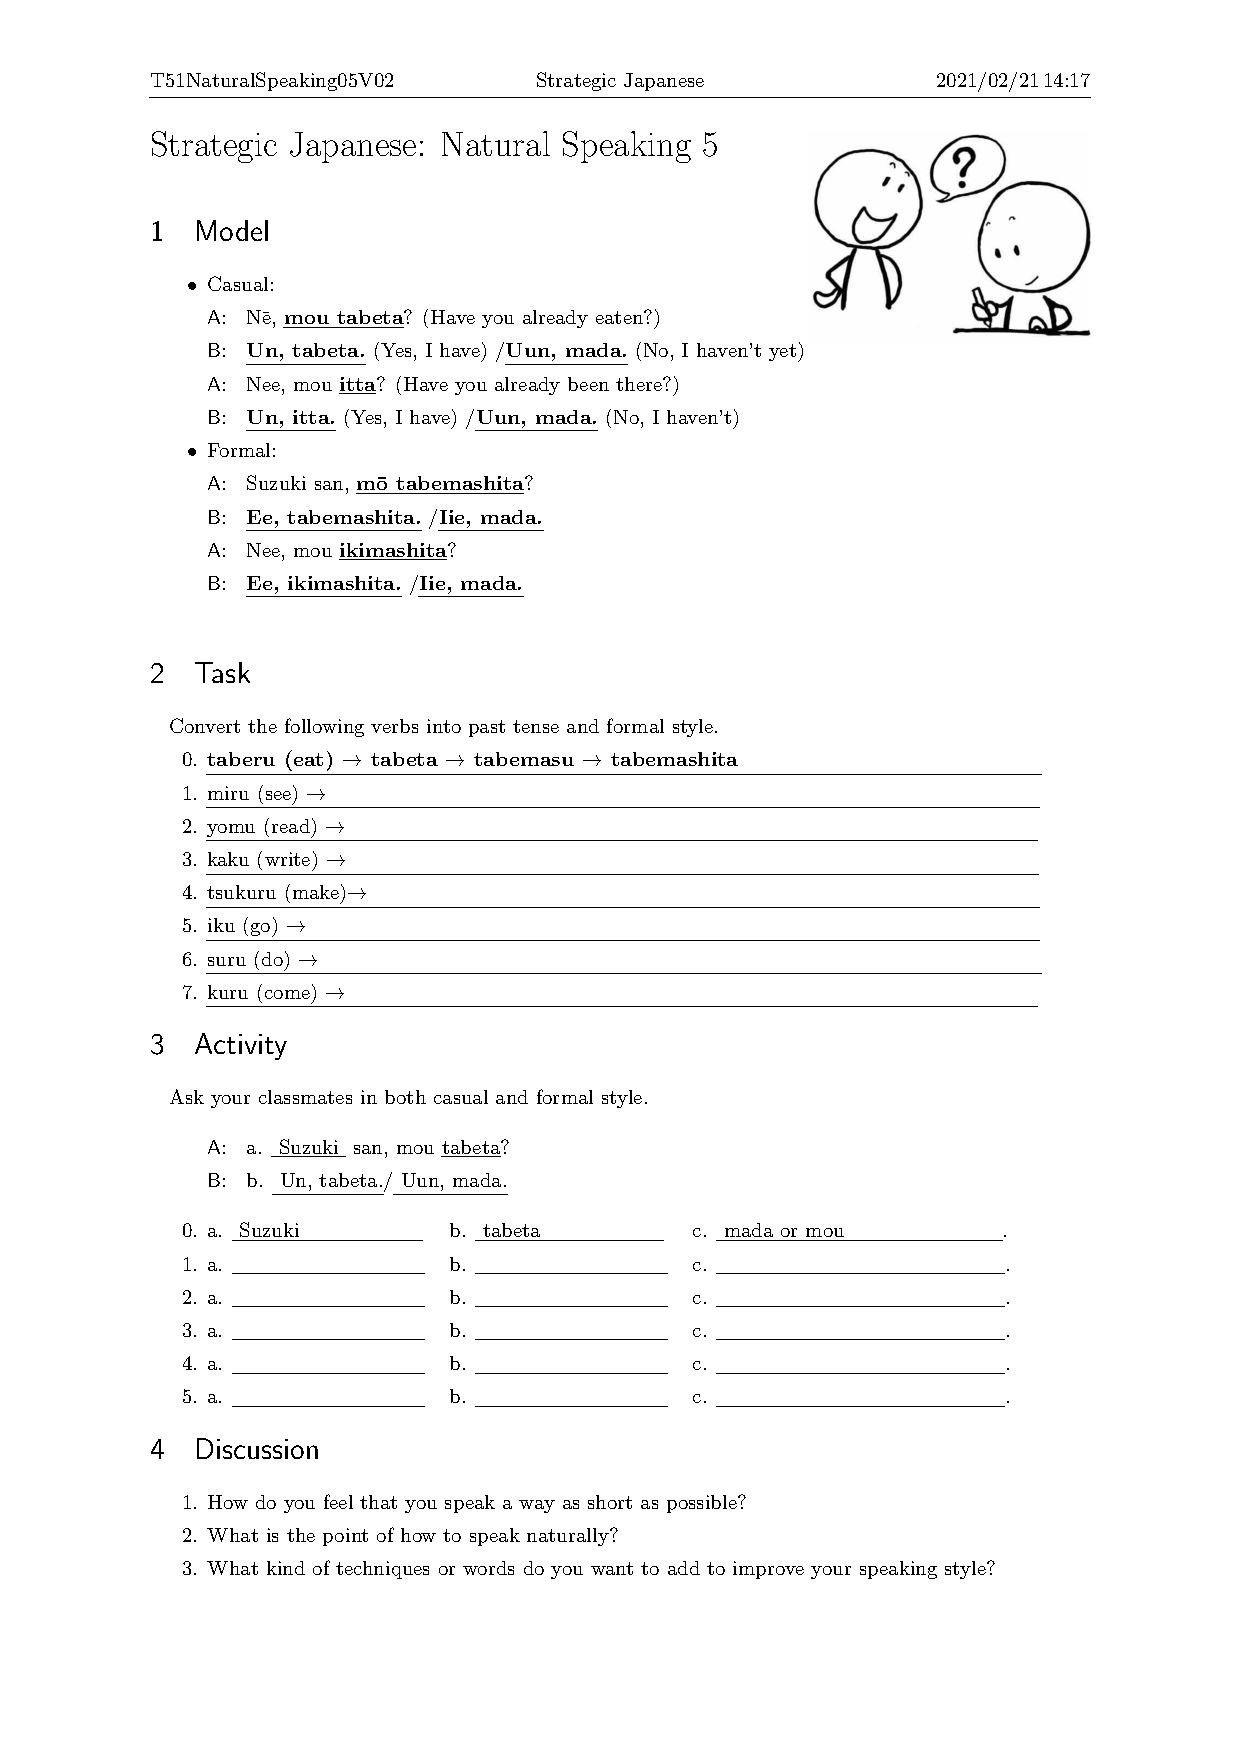
\includepdf[pages=-, scale=.86, trim=70 62 70 30, clip, offset=0mm -8.5mm, pagecommand={\thispagestyle{plain}}]{T51NaturalSpeaking05V02.pdf}

% 2022-08-16
\ifEnglish
  \section{Invitation}
\else
  \section{誘う・招待する}
\fi

%File: T51NaturalSpeaking06V02.pdf

\ifEnglish
\subsection{Model}
\else
\subsection{モデル}
\fi

\begin{toiquestion} % 2022-08-17
\ifEnglish
Find out what kinds of situations other than ``invite to dinner'' are available for inviting/inviting.
Also, observe what words are used when inviting someone.
\else
誘う・招待する場面は「食事に誘う」以外にどんな場面があるかを見つけなさい。
また、誘う・招待する場面ではどんなことばが使われるかを観察しなさい。
\fi
\end{toiquestion}

%たべいこ、たべよ
%たべにいきましょ、たべましょ

\begin{description}
\item Casual:
\begin{description}
 \item[A:] Nee, \underline{{\bfseries tabeiko / tabeyo}}? (Let's go to eat!)
 \item[B:] \underline{{\bfseries Un iko.}} (Yes, let's go) /\underline{{\bfseries Un, tabeyo.}} (Let's eat!)
\end{description}
\item Formal:
\begin{description}
 \item[A:] Suzuki san, issho ni \underline{{\bfseries tabeikimasho / tabemasho}}?
 \item[B:] \underline{{\bfseries Ee, ikimasho.}} /\underline{{\bfseries Ee, so shimasho.}}
\end{description}
\end{description}

%\ifILLUST
\begin{center}
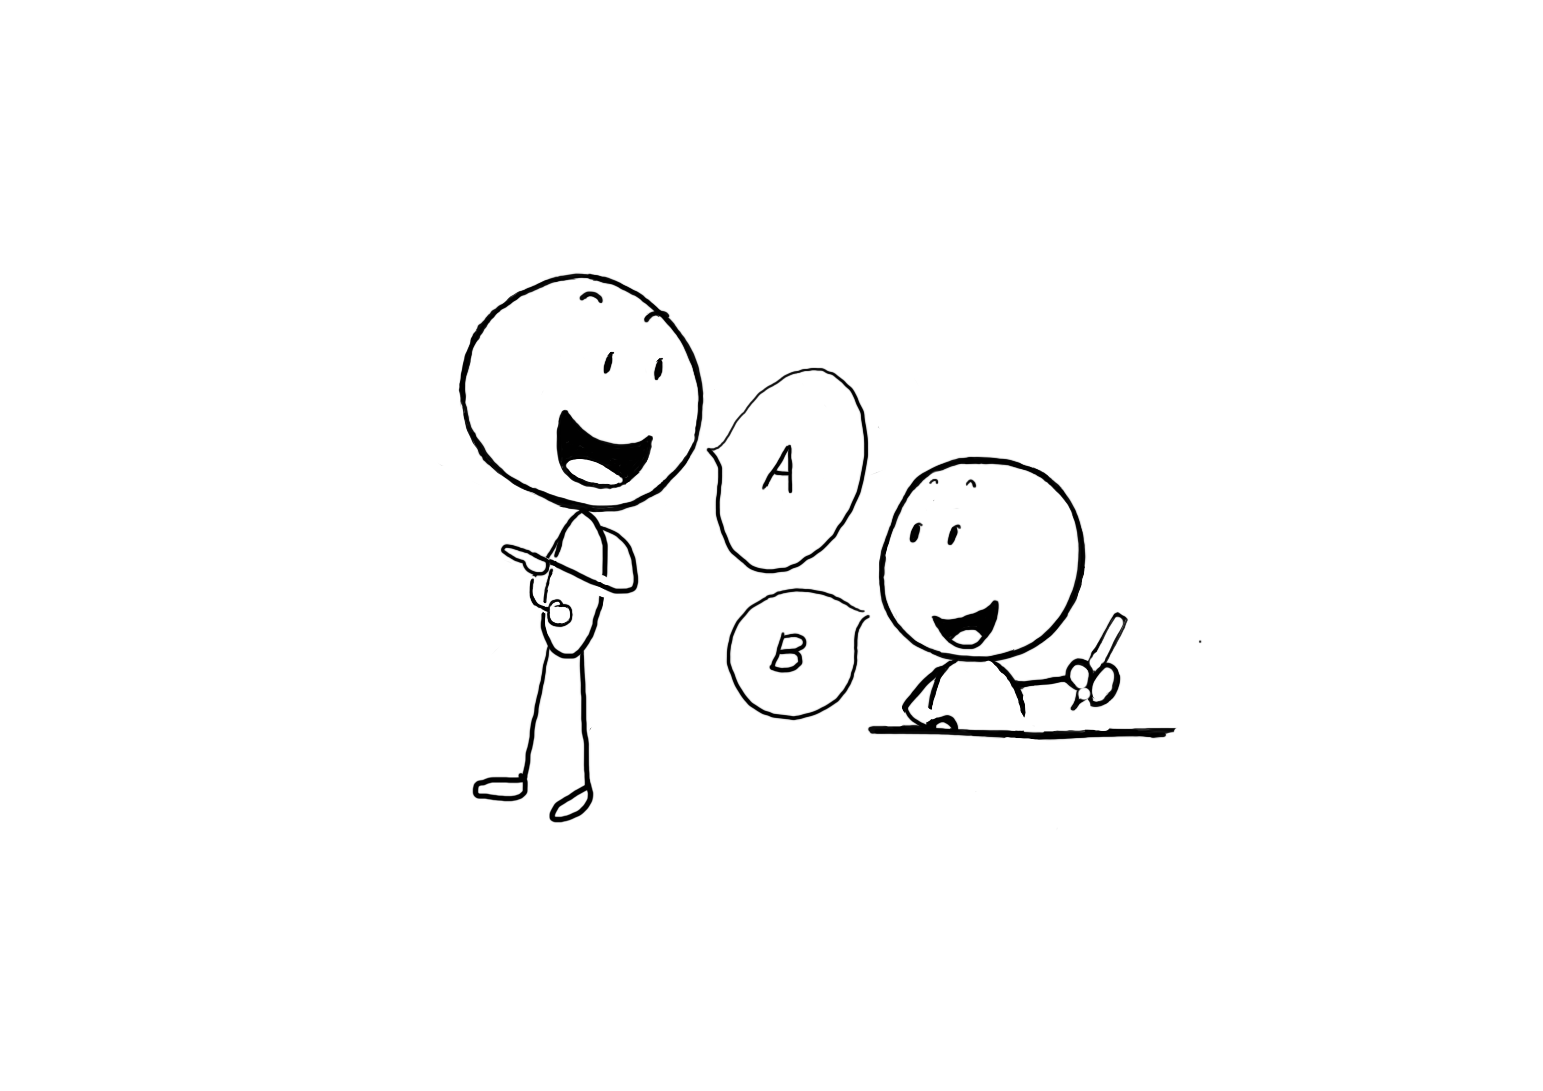
\includegraphics[trim=250 140 220 150, clip, width=.25\hsize]{img/naturalspeaking06.png}
\end{center}
\vspace*{0\baselineskip}
%\fi%ILLUST

\begin{toianswer}
\ifEnglish
You will learn casual and formal style using volitional verb form:
{\it tabe ni iko\/} (let's go to eat) is pronounced with {\it tabeiko\/} ({\it ni\/} is dropped and the word form is shortened), and {\it tabeyou\/} is shortend such as {\it tabeyo\/} which is a volitional form.
The contracted form is just how it sounds when it is actually pronounced, and it is convenient to learn how to make conjugations by learning it with its hiragana spellings.
See grammar notes for how to make intentional forms.$\rightarrow$ \S\ref{gn:volitional}
\else
意向形のカジュアル・スタイルとフォーマル・スタイルを学ぶ。
意向形の作り方は、Grammar notes (\S\ref{gn:volitional})を参照のこと。
「食べに行こう」は「たべいこ」、「食べよう」は「たべよ」として発音されることが多い。
「食べ行きましょう」は「食べいきましょ」として発音される。
縮約形は実際に発音されるときの聞こえ方であるだけで、活用形の作り方を学ぶためには平仮名の綴りで覚えるのが便利である。
\fi
\end{toianswer}

\ifEnglish
\subsection{Task}
\else
\subsection{タスク}
\fi

\begin{toiquestion}
\ifEnglish
Convert the following verbs into volitional casual and formal style.
\else
以下の動詞を意向形(カジュアルスタイルとフォーマルスタイル)に変換せよ。
\fi
\end{toiquestion}

\begin{enumerate}
 \item[0.] {\bfseries taberu (eat) $\rightarrow$ tabeiko $\rightarrow$ tabeyo $\rightarrow$ tabemasho}
 \item nomu (drink)  $\rightarrow$ \hrulefill
 \item yomu (read)   $\rightarrow$ \hrulefill
 \item kaku (write)  $\rightarrow$ \hrulefill
 \item tsukuru (make)$\rightarrow$ \hrulefill
 \item kiku (listen) $\rightarrow$ \hrulefill
 \item benkyosuru (study) $\rightarrow$ \hrulefill
 \item miru (see)    $\rightarrow$ \hrulefill
\end{enumerate}

\begin{toianswer}
\ifEnglish
In the case of {\it taberu\/} (eat), adding {\it ni iku\/} to {\it tabe\/} before {\it masu\/} of {\it tabemasu\/} gives {\it tabe ni iku\/} (go to eat).
Next, the volitional form of {\it iku\/} (go) is {\it ikou\/}, but if pronounced quickly, it becomes {\it iko\/}, and {\it u\/} is shortened and almost inaudible.
See grammar notes for how to create volitional forms.$\rightarrow$\S\ref{gn:volitional}
% {\bfseries taberu (eat) $\rightarrow$ tabeiko $\rightarrow$ tabeyo $\rightarrow$ tabemasho}

 {\it nomu\/} (drink) $\rightarrow$ {\it nomiiko\/} $\rightarrow$ {\it nomo\/} $\rightarrow$ {\it nomimasho\/};\\
 {\it yomu\/} (read) $\rightarrow$ {\it yomiiko\/} $\rightarrow$ {\it yomo\/} $\rightarrow$ {\it yomimasho\/};\\
 {\it kaku\/} (write) $\rightarrow$ {\it kakiiko\/} $\rightarrow$ {\it kako\/} $\rightarrow$ {\it kakimasho\/};\\
 {\it tsukuru\/} (make) $\rightarrow$ {\it tsukuriiko\/} $\rightarrow$ {\it tsukuro\/} $\rightarrow$ {\it tsukurimasho\/};\\
 {\it kiku\/} (listen) $\rightarrow$ {\it kikiiko\/} $\rightarrow$ {\it kiko\/} $\rightarrow$ {\it kikimasho\/};\\
 {\it benkyosuru\/} (study) $\rightarrow$ {\it benkyoshiiko\/} $\rightarrow$ {\it benkyoshiyo\/} $\rightarrow$ {\it benkyoshimasho\/};\\
 {\it miru\/} (see) $\rightarrow${\it miiko\/} $\rightarrow$ {\it miyo\/} $\rightarrow$ {\it mimasho\/}.
\else
「食べる」の場合は、「食べます」の「ます」の前の形「食べ」に「に行く」を付けると「食べに行く」となる。
次に「行く」の意向形は「行こう」であるが、速く発音すると「行こ」になり、「う」が短かくなり、ほとんど聞こえなくなる。
意向形の作り方は\S\ref{gn:volitional}を参照のこと。
\fi
\end{toianswer}

\ifEnglish
\subsection{Activity}
\else
\subsection{アクティビティ}
\fi

\begin{toiquestion}
\ifEnglish
Ask your classmates in both casual and formal style.
\else
カジュアルとフォーマルスタイルでクラスメイトに質問しなさい。
\fi
\end{toiquestion}

\begin{description}
 \item[A:] a)\underline{ Suzuki } san, b)\underline{tabeiko}?
 \item[B:] c)\underline{ Un, iko.}/\underline{ Un, tabeyo.}
\end{description}

\begin{enumerate}
  \item[0.] a.\underline{ Suzuki\hspace{6.5zw}} b.\underline{ tabeiko\hspace{6.2zw}} c.\underline{ un tabeyo\hspace{7.0zw}}.
  \item a.\underline{\hspace{10zw}} b.\underline{\hspace{10zw}}  c.\underline{\hspace{12zw}}.
  \item a.\underline{\hspace{10zw}} b.\underline{\hspace{10zw}}  c.\underline{\hspace{12zw}}.
  \item a.\underline{\hspace{10zw}} b.\underline{\hspace{10zw}}  c.\underline{\hspace{12zw}}.
  \item a.\underline{\hspace{10zw}} b.\underline{\hspace{10zw}}  c.\underline{\hspace{12zw}}.
  \item a.\underline{\hspace{10zw}} b.\underline{\hspace{10zw}}  c.\underline{\hspace{12zw}}.
\end{enumerate}

\begin{toianswer}
\ifEnglish
Using the word {\it isshoni\/} (together) is also a good idea.
It's also a good idea to practice using words like {\it eiga\/} (movie) and {\it hanabi\/} (fireworks) when you go to see it.
\else
「いっしょに」という語を使うのもよいアイデアである。
「見に行こ」のときには、「映画」「花火」のような語を使って練習してみるのもよい。
\fi
\end{toianswer}

\ifEnglish
\subsection{Discussion}
\else
\subsection{ディスカッション}
\fi

\begin{toiquestion}
\ifEnglish
How do you feel when you speak naturally in this way?
\else
このように自然に話せるようになってどんな感じがするか?
\fi
\end{toiquestion}
\begin{toianswer}
\ifEnglish
As the interaction continues, you will start to feel like you are having a real conversation, and you will gradually gain confidence.
You will be happy if you can feel that you are really speaking Japanese by yourself.
Just like your mother tongue, natural conversations are those which you can speak without preparation.
\else
やりとりが続くと会話している感じが出てきて、だんだん自信が付くだろう。
本当に自分ひとりで日本語を話していることが実感できるとうれしくなるだろう。
自分の母語と同じで、自然な会話は準備しないで話せる会話である。
\fi
\end{toianswer}


\begin{toiquestion}
\ifEnglish
What is the point of how to speak naturally?
\else
自然な話し方のコツとは何か。
\fi
\end{toiquestion}
\begin{toianswer}
\ifEnglish
What works for you may not necessarily work for others.
But sharing what worked and what didn't worked for you can help you refine your learning.
\else
自分がうまくいった方法が他の人にとってもうまくいく方法であるとは限らない。
しかし、自分がうまくいった方法やうまくいかなかった方法を共有することは学び方を工夫する点で役に立つ。
\fi
\end{toianswer}

\begin{toiquestion}
\ifEnglish
What words and techniques should you learn further to be a better speaker?
\else
話が上手になるにはどんな単語、どんなテクニックをさらに学ぶとよいか。
\fi
\end{toiquestion}
\begin{toianswer}
\ifEnglish
It is important to use the same words and expressions many times.
You can't say the same thing to the same person over and over again, so it's good to create an environment where you can talk to multiple people.
Proactively going to parties and meetings and creating opportunities to meet different people is more important than learning different words and expressions.
\else
同じ語や表現を何回も使うことが重要である。
同じ人に同じことを何回も言えないので、複数の人と話ができる環境を作るとよい。
パーティやミーティングに積極的に出かけて、いろいろな人と合うチャンスを作ることが、さまざまな語や表現を覚えるより重要である。
\fi
\end{toianswer}


%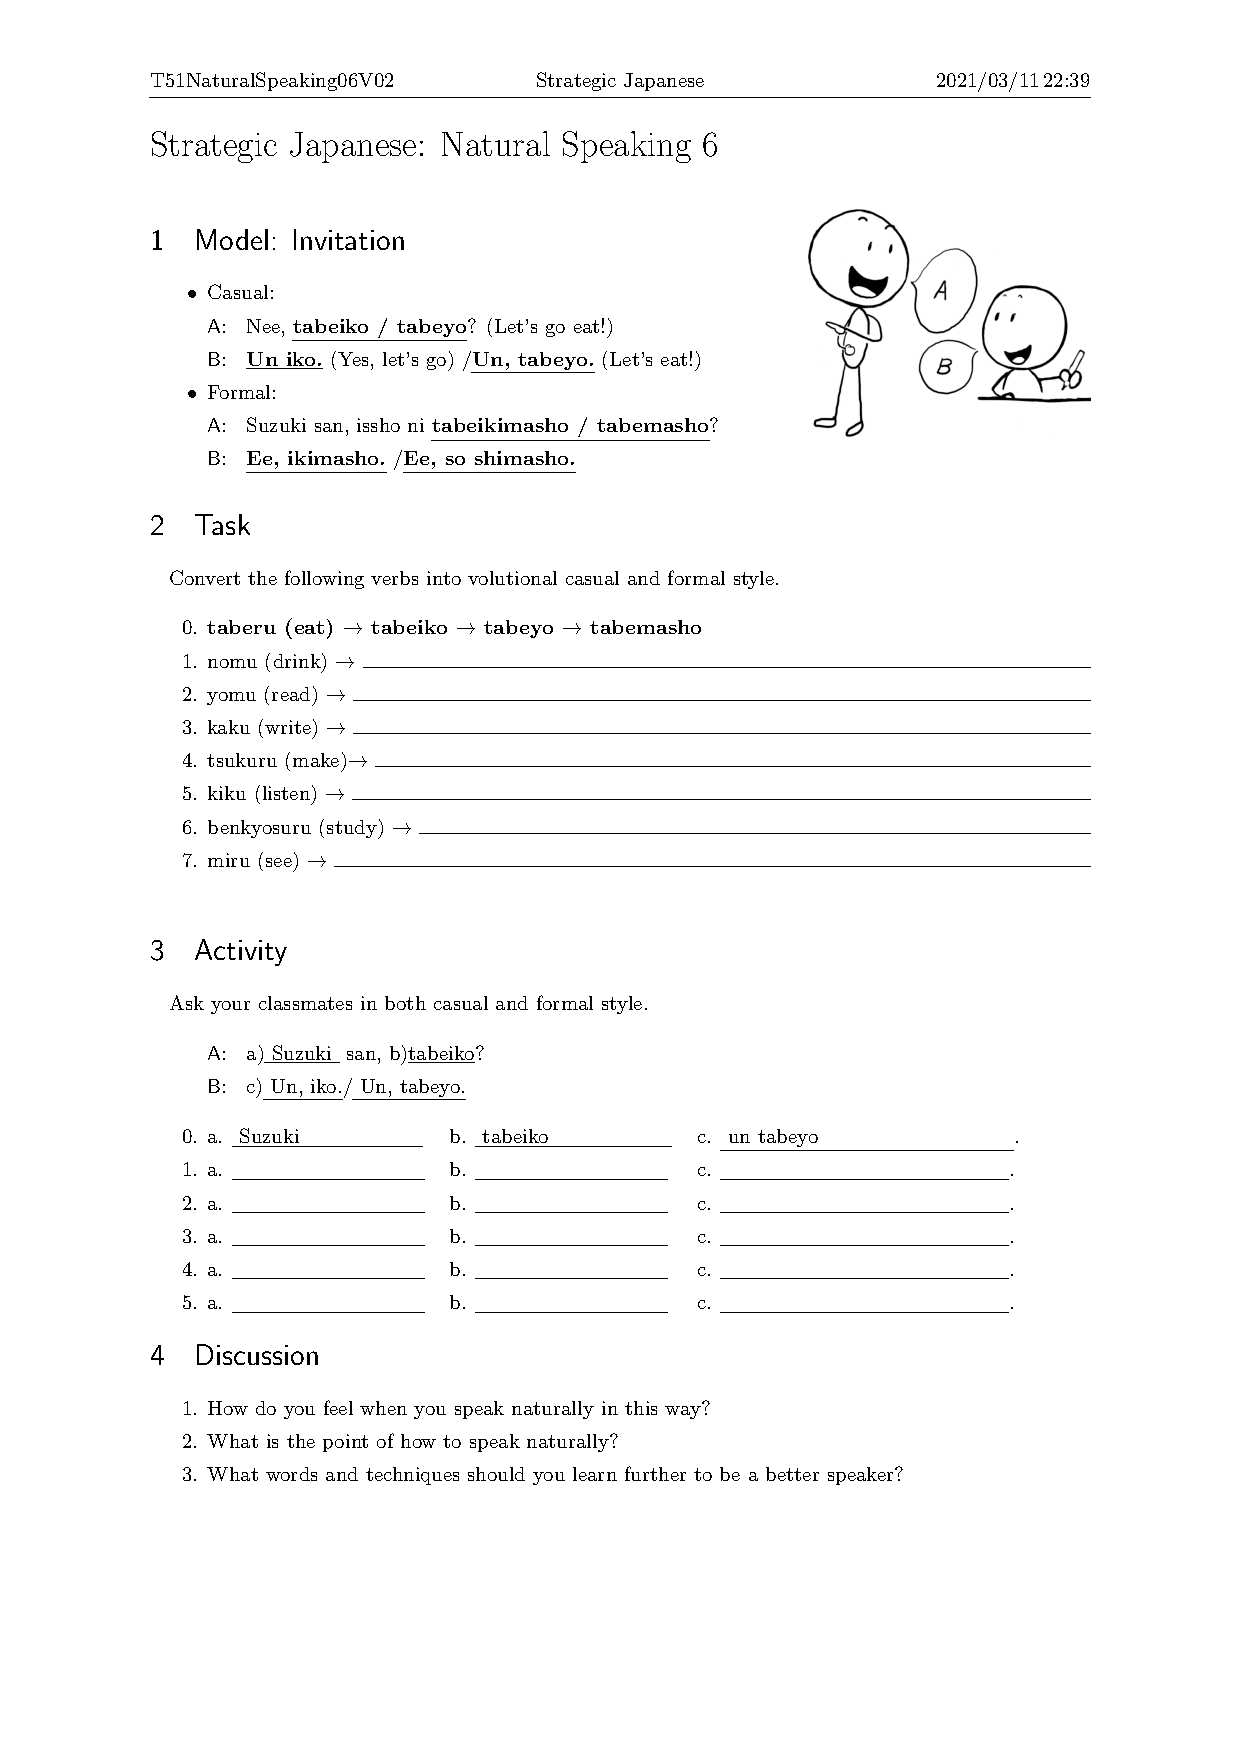
\includepdf[pages=-, scale=.86, trim=70 62 70 30, clip, offset=0mm -8.5mm, pagecommand={\thispagestyle{plain}}]{T51NaturalSpeaking06V02.pdf}

\ifEnglish
\section{Asking and reacting}
\else
\section{説得と反応}
\fi

\ifEnglish
Volitional, negative, and conditional form of verb;
``j\=a tabere ba'' (you can if you want) is a kind of rude expression but it is often used between two friends.
\else
意向形、否定形、条件形、
「じゃ、すればぁ〜」は少々ぞんざいな言い方、しかし、友達関係ではよく使う。
\fi

%File: T51NaturalSpeaking07V02.pdf

\ifEnglish
\subsection{Model}
\else
\subsection{モデル}
\fi

\begin{toiquestion}
\ifEnglish
Look at the following conversation patterns and discuss how each one makes you feel.
\else
次の会話のパターンを見て、それぞれどんな感じがするかを話し合いなさい。
\fi
\end{toiquestion}

\begin{itemize}
 \item[A:] N\=e, \underline{{\bfseries tabeyo}}? (We gonna eat this)
 \item[B:] \underline{{\bfseries Ja tabeyo.}} (OK! I will)
 \item[A:] Kore \underline{{\bfseries tabeyo}}? (Let's eat this!)
 \item[C:] \underline{{\bfseries Uun tabenai.}} (No, I don't)
 \item[A:] Kore \underline{{\bfseries tabeyo}}? (Let's eat this!)
 \item[D:] \underline{{\bfseries Uun ima wa chotto..}} (Uum..not now)
 \item[A:] N\=e, \underline{{\bfseries tabeyo}}? (We gonna eat this)
 \item[E:] \underline{{\bfseries J\=a tabereba.}} (You can if you want, but I don't)
\end{itemize}

\begin{toianswer}
\ifEnglish
{\it Ba\/} in {\it tabereba\/} is a conditional expression.
\else
「食べれば」の「ば」は条件の表現である。
\fi
\ifEnglish
Use E only when talking to friends.
\else
Eを使うときは、友達に話すときに限ること。
\fi
\end{toianswer}

%\ifILLUST
\vspace*{-10\baselineskip}
\begin{flushright}
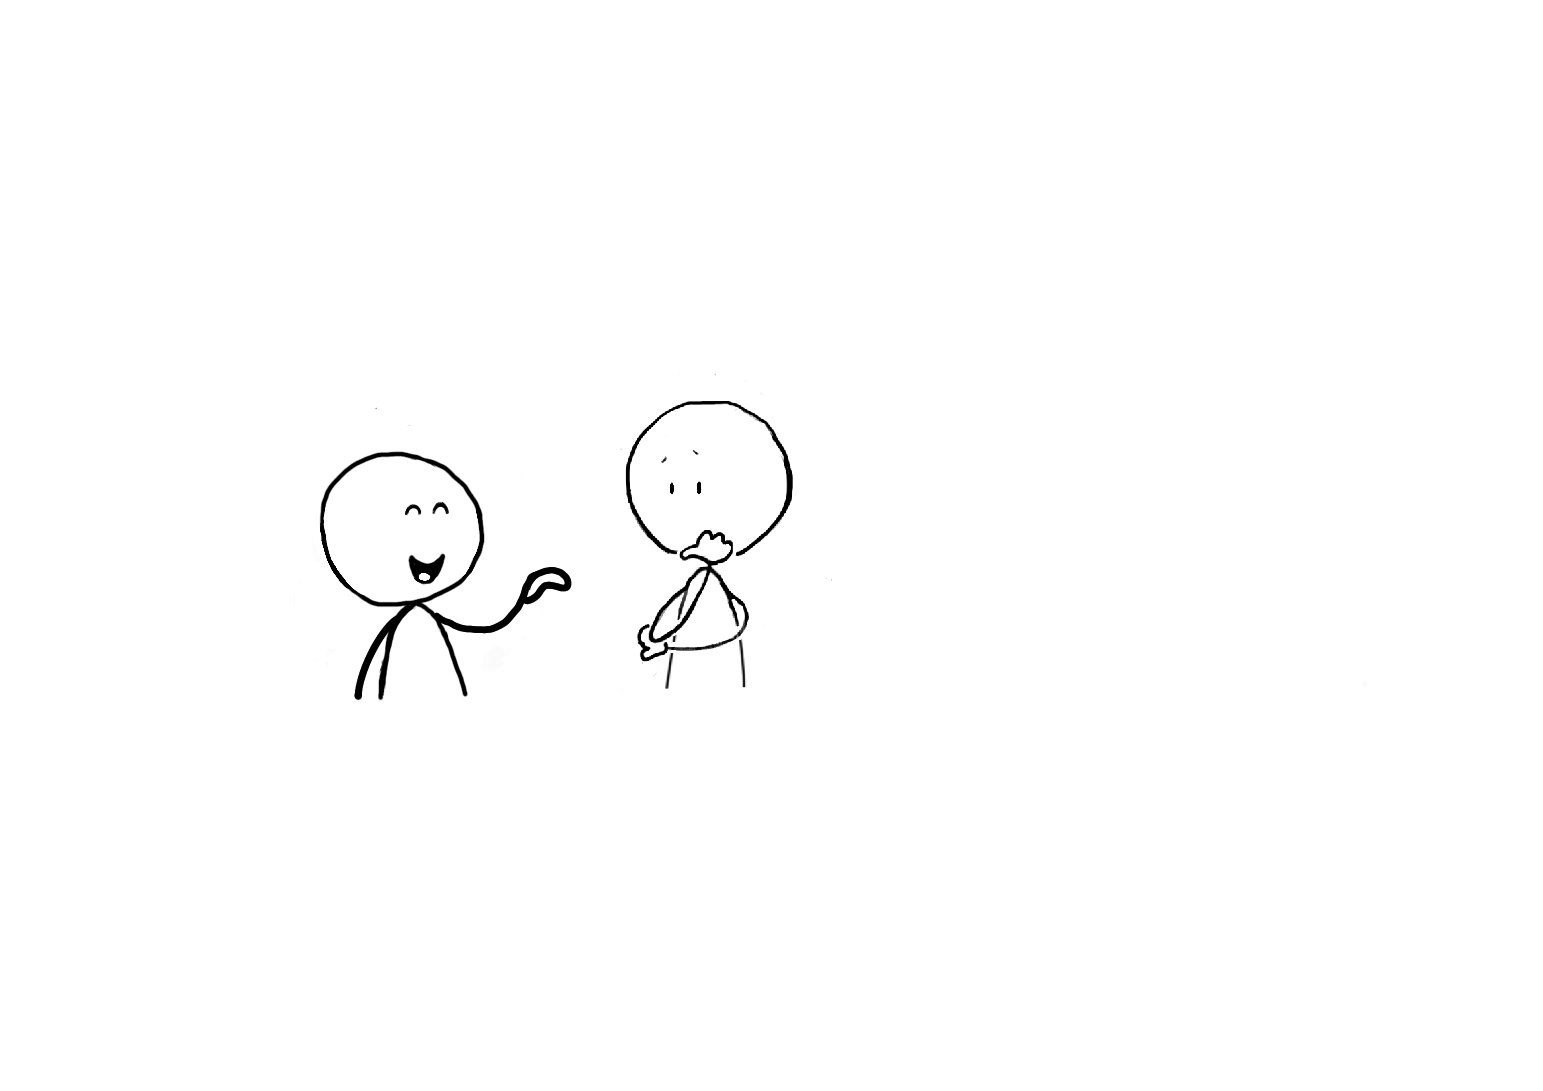
\includegraphics[trim=170 200 400 200, clip, width=.3\hsize]{img/sureba.png}
\end{flushright}
\vspace*{2\baselineskip}
%\fi%ILLUST

\ifEnglish
\subsection{Task}
\else
\subsection{タスク}
\fi

\begin{toiquestion}
\ifEnglish
Convert the following verbs into volitional form, negative form, and conditional form.
\else
以下の動詞を、意向形、否定形、条件形に変換せよ。
\fi
\end{toiquestion}

\begin{enumerate}
 \item[0.] {\bfseries taberu (eat) $\rightarrow$ tabeyo $\rightarrow$ tabenai $\rightarrow$ tabereba}
 \item nomu (drink)  $\rightarrow$ \hrulefill
 \item yomu (read)   $\rightarrow$ \hrulefill
 \item kaku (write)  $\rightarrow$ \hrulefill
 \item tsukuru (make)$\rightarrow$ \hrulefill
 \item kiku (listen) $\rightarrow$ \hrulefill
 \item benkyosuru (study) $\rightarrow$ \hrulefill
 \item miru (see)    $\rightarrow$ \hrulefill
 \item karaoke iku (go to karaoke) $\rightarrow$ \hrulefill
\end{enumerate}

\begin{toianswer}
\begin{enumerate}
\ifEnglish
 \item[0.] {\bfseries taberu (eat) $\rightarrow$ tabeyo $\rightarrow$ tabenai $\rightarrow$ tabereba}
 \item nomu        $\rightarrow$ nomo $\rightarrow$ nomanai $\rightarrow$ nomeba
 \item yomu        $\rightarrow$ yomo $\rightarrow$ yomanai $\rightarrow$ yomeba
 \item kaku        $\rightarrow$ kako $\rightarrow$ kakanai $\rightarrow$ kakeba
 \item tsukuru     $\rightarrow$ tsukuro $\rightarrow$ tsukuranai $\rightarrow$ tsukureba
 \item kiku        $\rightarrow$ kiko $\rightarrow$ kikanai $\rightarrow$ kikeba
 \item benkyosuru  $\rightarrow$ benkyoshiyo $\rightarrow$ benkyoshinai $\rightarrow$ benkyosureba
 \item miru        $\rightarrow$ miyo $\rightarrow$ minai $\rightarrow$ mireba
 \item karaoke iku $\rightarrow$ karaoke iko $\rightarrow$ karaoke ikanai $\rightarrow$ karaoke ikeba
\else
 \item[0.] {\bfseries taberu (eat) $\rightarrow$ tabeyo $\rightarrow$ tabenai $\rightarrow$ tabereba}
 \item nomu (drink)  $\rightarrow$
 \item yomu (read)   $\rightarrow$
 \item kaku (write)  $\rightarrow$
 \item tsukuru (make)$\rightarrow$
 \item kiku (listen) $\rightarrow$
 \item benkyosuru (study) $\rightarrow$
 \item miru (see)    $\rightarrow$
 \item karaoke iku (go to karaoke) $\rightarrow$
\fi
\end{enumerate}
\end{toianswer}



\ifEnglish
\subsection{Activity}
\else
\subsection{アクティビティ}
\fi

\begin{toiquestion}
\ifEnglish
ask and invite your classmates.
\else
クラスメイトを説得せよ。
\fi
\end{toiquestion}

\begin{description}
 \item[A:] a.\underline{ Suzuki } san,  N\=e, b.\underline{sushi} c.\underline{tabeyo}?
 \item[B:] d.\underline{ Un, tabenai.}/\underline{ Ja, tabeyo.}/\underline{ J\=a, tabereba.}
\end{description}

\begin{tabular}[t]{llll}
 0. a. \underline{ Suzuki\hspace{2.5zw}}
 &  b. \underline{ sushi\hspace{3.3zw}}
 &  c. \underline{ tabeiko\hspace{2.0zw}}
 &  d. \underline{ j\=a tabereba\hspace{0.5zw}}.\\
 1. a. \underline{\hspace{6zw}}& b. \underline{\hspace{6zw}} & c. \underline{\hspace{6zw}} & d. \underline{\hspace{6zw}}.\\
 2. a. \underline{\hspace{6zw}}& b. \underline{\hspace{6zw}} & c. \underline{\hspace{6zw}} & d. \underline{\hspace{6zw}}.\\
 3. a. \underline{\hspace{6zw}}& b. \underline{\hspace{6zw}} & c. \underline{\hspace{6zw}} & d. \underline{\hspace{6zw}}.\\
 4. a. \underline{\hspace{6zw}}& b. \underline{\hspace{6zw}} & c. \underline{\hspace{6zw}} & d. \underline{\hspace{6zw}}.\\
 5. a. \underline{\hspace{6zw}}& b. \underline{\hspace{6zw}} & c. \underline{\hspace{6zw}} & d. \underline{\hspace{6zw}}.\\
 6. a. \underline{\hspace{6zw}}& b. \underline{\hspace{6zw}} & c. \underline{\hspace{6zw}} & d. \underline{\hspace{6zw}}.\\
 7. a. \underline{\hspace{6zw}}& b. \underline{\hspace{6zw}} & c. \underline{\hspace{6zw}} & d. \underline{\hspace{6zw}}.\\
\end{tabular}

\begin{toianswer}
\ifEnglish
Check how to create the conditional form.
\else
条件形の作り方を確認しておく。
\fi
\end{toianswer}

\ifEnglish
\subsection{Discussion}
\else
\subsection{ディスカッション}
\fi
% 2022-08-21

\begin{toiquestion}
\ifEnglish
Make sure how to conjugate verbs.
\else
動詞の活用形を確認せよ。
\fi
\end{toiquestion}
\begin{toianswer}
\ifEnglish
In this section, you only learned how to create conditional forms.
You will learn how to use the conditional form in a later chapter.
\else
このセクションでは、条件形の作り方のみを学んだ。
条件形の具体的な使い方は後の章で学ぶ。
\fi
\end{toianswer}

\begin{toiquestion}
\ifEnglish
What kind of game can you invent for learning Japanese verb conjugation?
\else
日本語の動詞の活用を学ぶために、どのようなゲームが考案できるか。
\fi
\end{toiquestion}
\begin{toianswer} % 2022-08-23
\ifEnglish
Ask the problem and answer the solution.
Play {\it ..ba ii\/} game.
\else
問題を尋ねて、解決策を回答する。
「~ばいい」ゲームを行なう。
\fi
\begin{enumerate}
\ifEnglish
\item What do you do when you don't have money?
\item What do you do when you have a lot of homework?
\item What do you do when you're hungry?
\item what do you do when you are busy in the morning?
\item What do you do when you don't know a word?
\else
\item お金がないとき、どうする。
\item 宿題が多いとき、どうする。
\item お腹がへったとき、どうする。
\item 朝、忙しいとき、どうする。
\item 単語がわからないとき、どうする。
\fi
\end{enumerate}

\end{toianswer}


%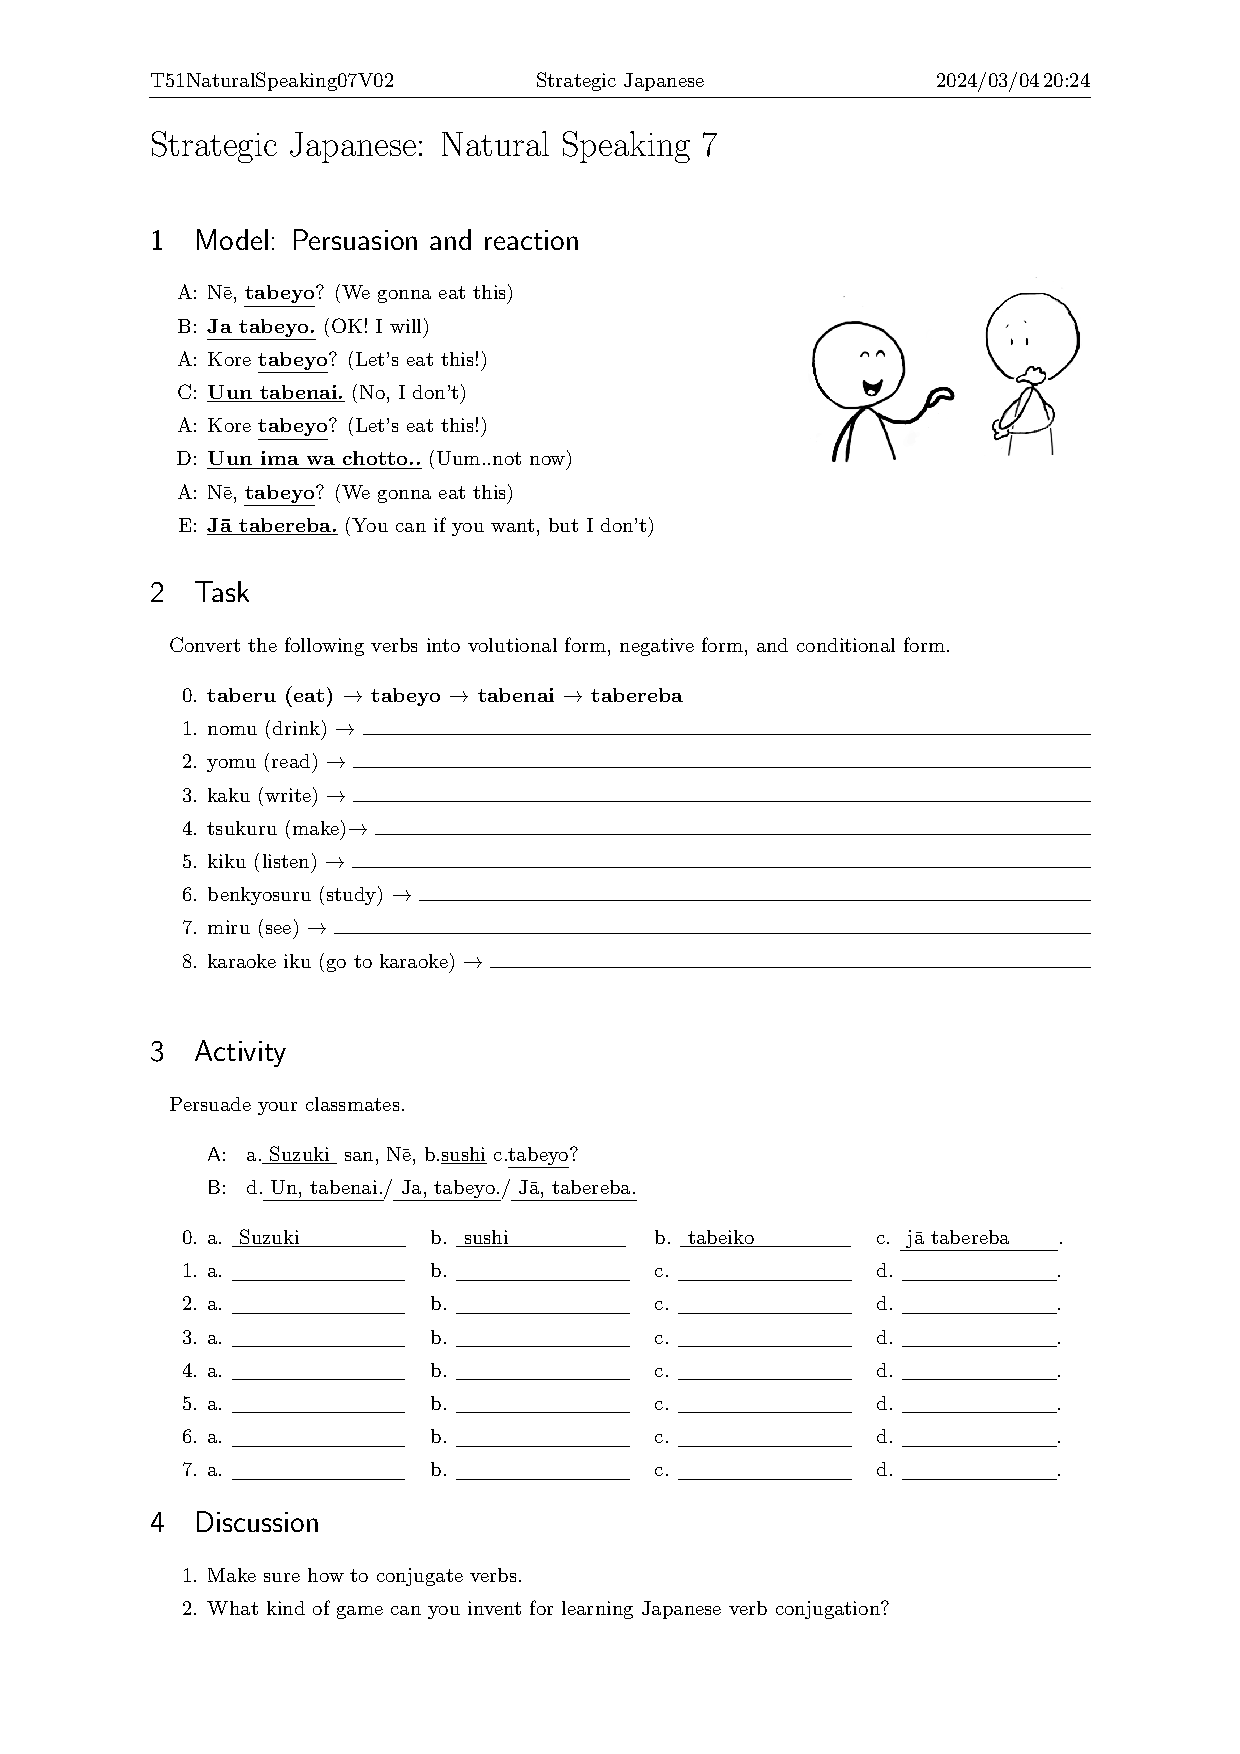
\includepdf[pages=-, scale=.86, trim=70 62 70 30, clip, offset=0mm -8.5mm, pagecommand={\thispagestyle{plain}}]{T51NaturalSpeaking07V02.pdf}

\ifEnglish
\section{Reporting a progressive situation}
\else
\section{進行中のことを報告する}
\fi

%File: T51NaturalSpeaking08V02.pdf


\ifEnglish
\subsection{Model}
\else
\subsection{モデル}
\fi

\ifEnglish
Learn the progressive tense and progressive form of verb {\it nani shiteru\/} (what are you doing?)
\else
進行形「何してる」を学ぶ。
\fi

\begin{itemize}
 \item[A:] Nani {\bfseries shiteru?} (What are you doing?)
 \item[B:] Ima, {\bfseries tabeteru.} (I'm eating now)\\
	   \underline{Kar\=eraisu}, isshoni {\bfseries d\=o?} (How about eating curry rice together?)
 \item[A:] {\bfseries Un} (Yes!)/{\bfseries \=Un yametoku} (No, no thank you)
\end{itemize}

\begin{center}
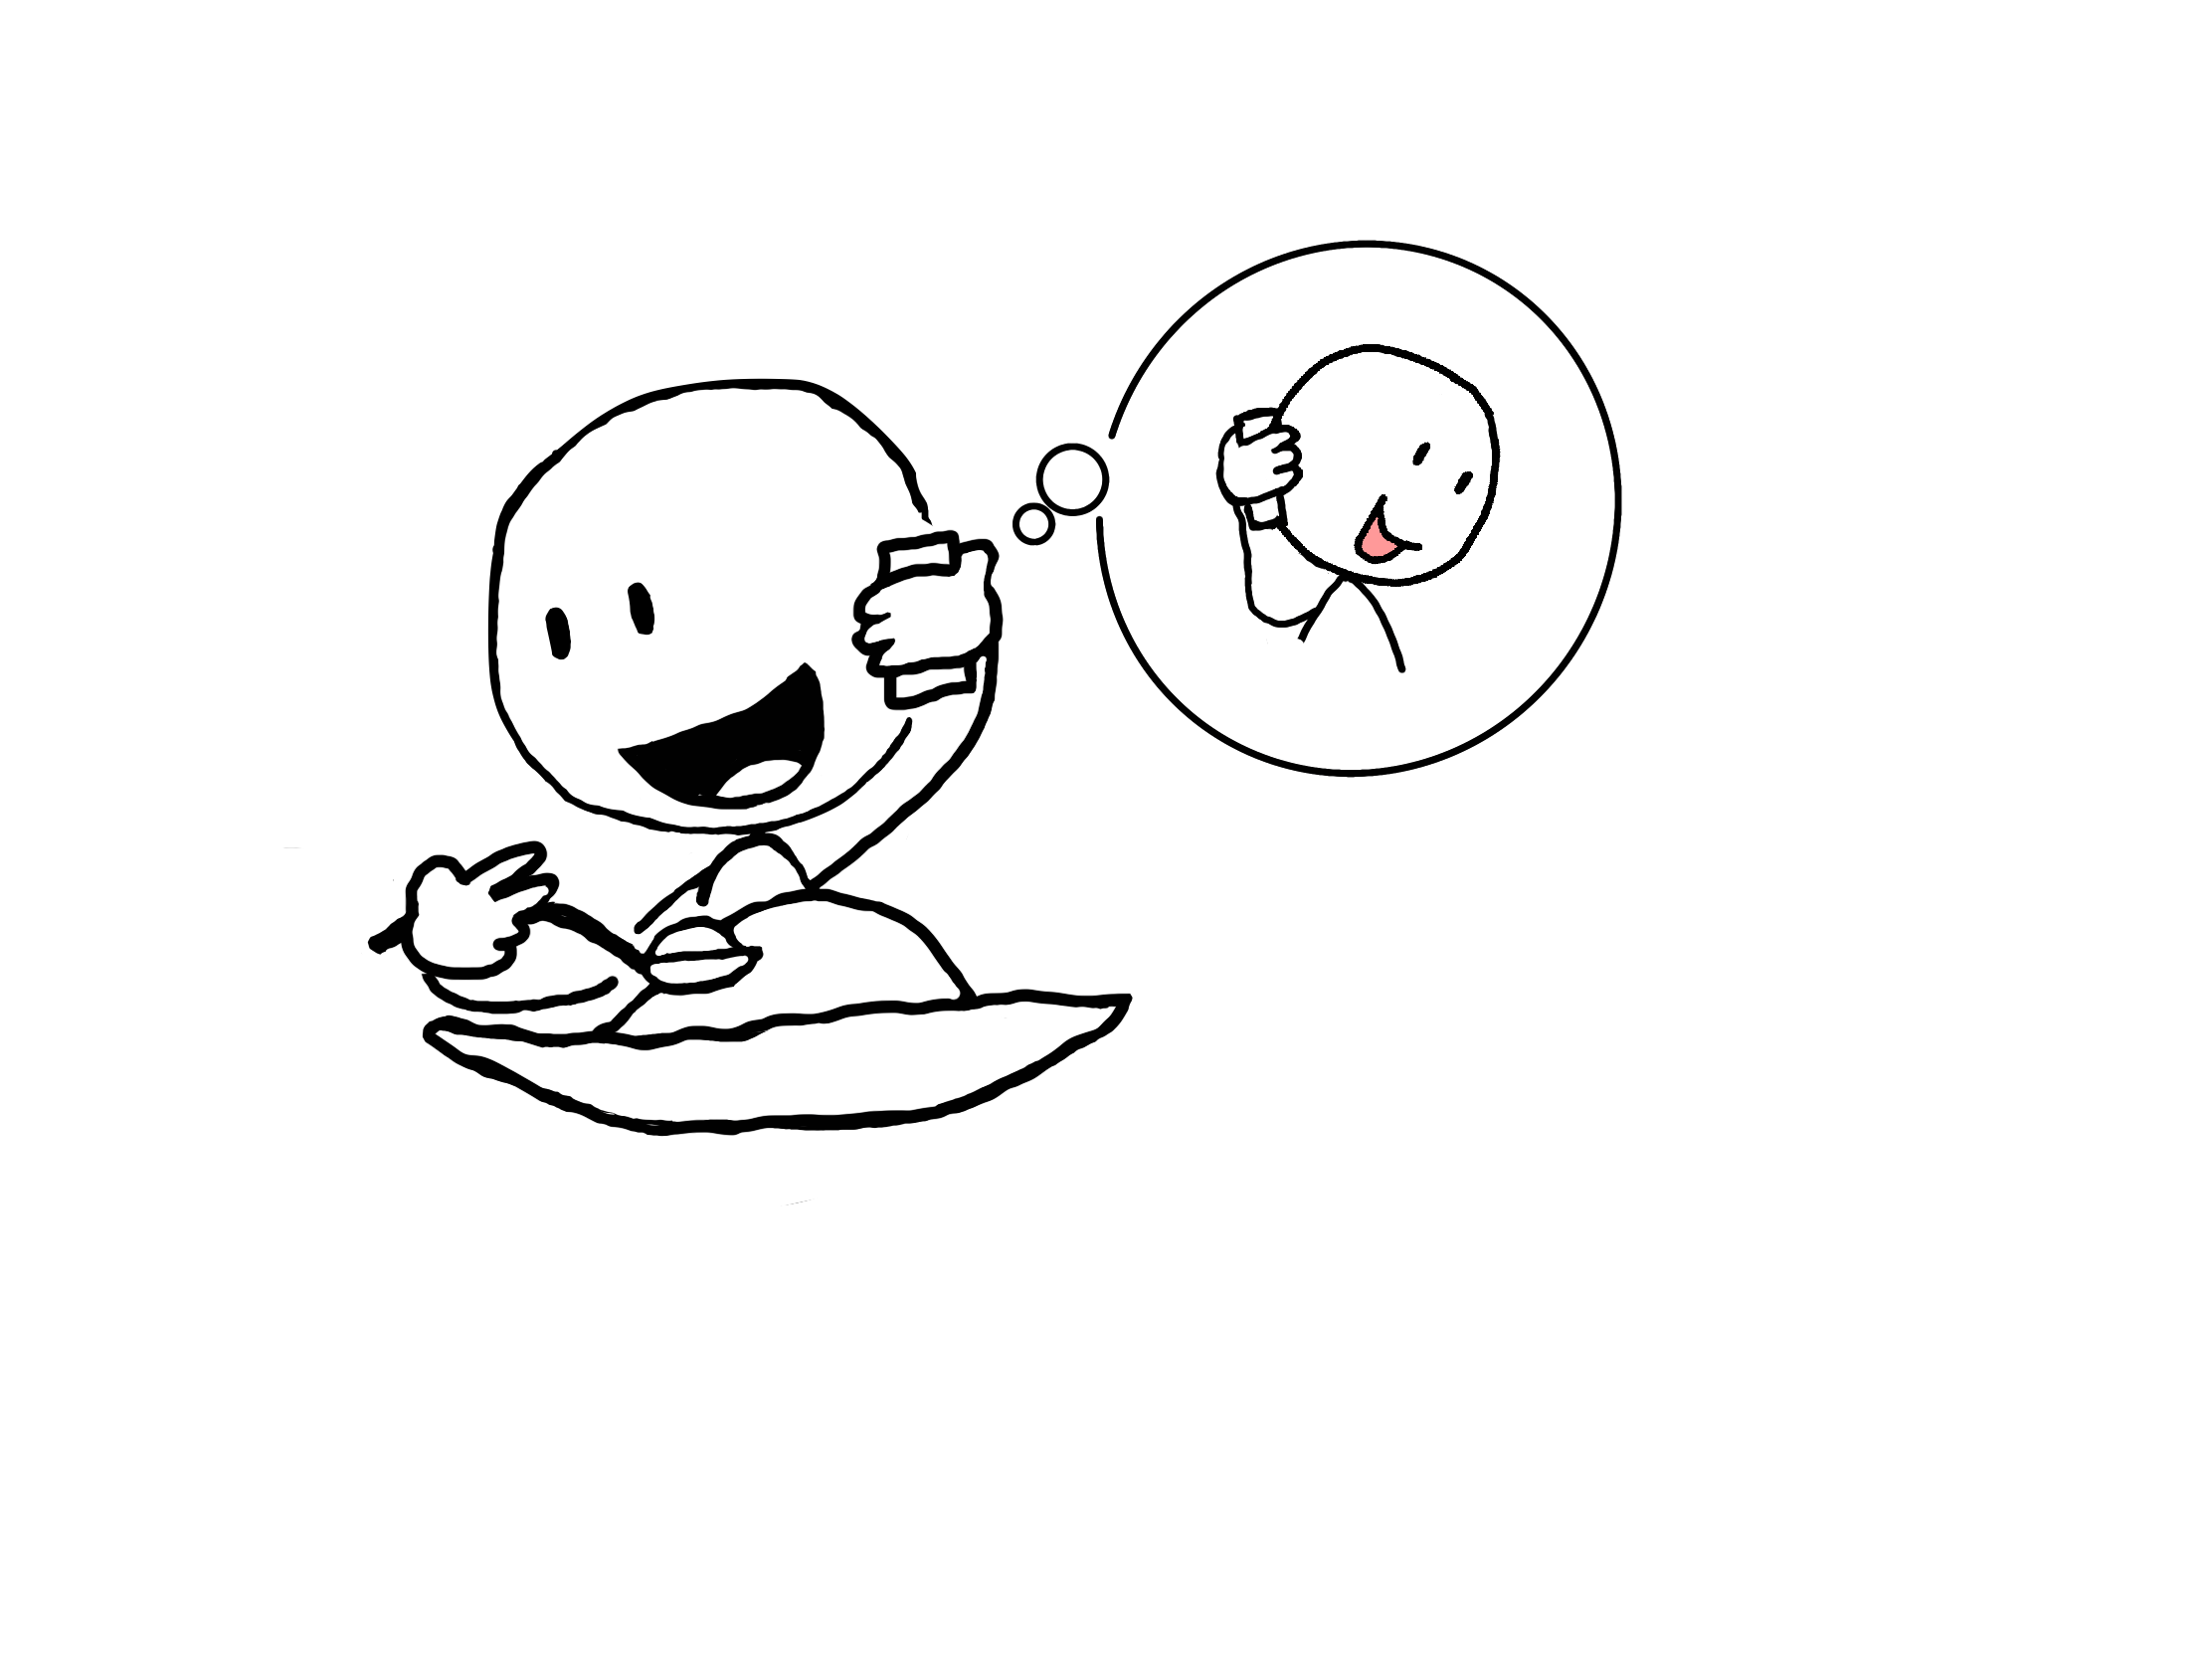
\includegraphics[trim=70 100 120 50, clip, width=.3\hsize]{img/nanishiteru.png}
\end{center}

\ifEnglish
\subsection{Task}
\else
\subsection{タスク}
\fi

\begin{toiquestion}
\ifEnglish
Convert the following verbs into a progressing form (V-teiru/V-teru).
\else
動詞を進行形(V-teiru/V-teru)に変換する。
\fi
\end{toiquestion}

\begin{multicols}{2}
 \begin{enumerate}
 \setcounter{enumi}{-1}
 \item taberu (eat)   $\rightarrow$ tabeteiru / tabeteru \hrulefill
 \item suru (do) $\rightarrow$ \hrulefill
 \item kuru (come)   $\rightarrow$ \hrulefill
 \item dekakeru (leave) $\rightarrow$ \hrulefill
 \item miru (see)  $\rightarrow$ \hrulefill
 \item tsukuru (make) $\rightarrow$ \hrulefill
 \item kau (buy)   $\rightarrow$ \hrulefill
 \item kaku (write)  $\rightarrow$ \hrulefill
 \item iku (go)   $\rightarrow$ \hrulefill
 \item yomu (read)   $\rightarrow$ \hrulefill
 \item nomu (drink)   $\rightarrow$ \hrulefill
 \item mottekuru (bring)   $\rightarrow$ \hrulefill
 \end{enumerate}
\end{multicols}

\vspace*{-1\baselineskip}

\begin{toiquestion}
\ifEnglish
Write nouns or verbs you are doing.
\else
名詞あるいは自分がやっている動詞を書く。
\fi
\end{toiquestion}

\begin{multicols}{2}
\begin{enumerate}
 \setcounter{enumi}{-1}
 \item Benky\=o $\rightarrow$ Benky\=o, isshoni d\=o?
 \item \hrulefill
 \item \hrulefill
 \item \hrulefill
 \item \hrulefill
 \item \hrulefill
 \item \hrulefill
 \item \hrulefill
\end{enumerate}
\end{multicols}

\vspace*{-1\baselineskip}

\ifEnglish
\subsection{Activity}
\else
\subsection{アクティビティ}
\fi

\begin{toiquestion}
\ifEnglish
Have a conversation with classmates and take notes.
\else
クラスメートと会話をして、メモを取る。
\fi
\end{toiquestion}

\begin{itemize}
 \item[A:] a.\underline{ Suzuki san }! Nani shiteru?
 \item[B:] b.\underline{ Kar\=eraisu tabeteru }. Isshoni d\=o?
 \item[A:] c.\underline{ Un! / Uun yametoku }.
\end{itemize}

\begin{enumerate}
 \setcounter{enumi}{-1}
 \item a.\underline{ Suzuki\hspace{5zw}}, b.\underline{ eating a curry rice\hspace{4.0zw}}, c.\underline{ no thank you\hspace{4.4zw}}.
 \item a.\underline{\hspace{8.5zw}}, b.\underline{\hspace{13zw}}, c.\underline{\hspace{11zw}}.
 \item a.\underline{\hspace{8.5zw}}, b.\underline{\hspace{13zw}}, c.\underline{\hspace{11zw}}.
 \item a.\underline{\hspace{8.5zw}}, b.\underline{\hspace{13zw}}, c.\underline{\hspace{11zw}}.
\end{enumerate}

\ifEnglish
\subsection{Discussion}
\else
\subsection{ディスカッション}
\fi

\begin{toiquestion}
\ifEnglish
Under what circumstances can this conversation be used?
\else
どのような場合にこの会話が使えるのか?
\fi
\end{toiquestion}

\begin{toiquestion}
\ifEnglish
If you use this tonight, which topic would you apply to this conversation?
\else
今夜これを使うとしたら、どの話題をこの会話に活用するか?
\fi
\end{toiquestion}

\begin{toiquestion}
\ifEnglish
Please tell us an interesting use of this grammar.
\else
この文法の面白い使い方を考えよ。
\fi
\end{toiquestion}



%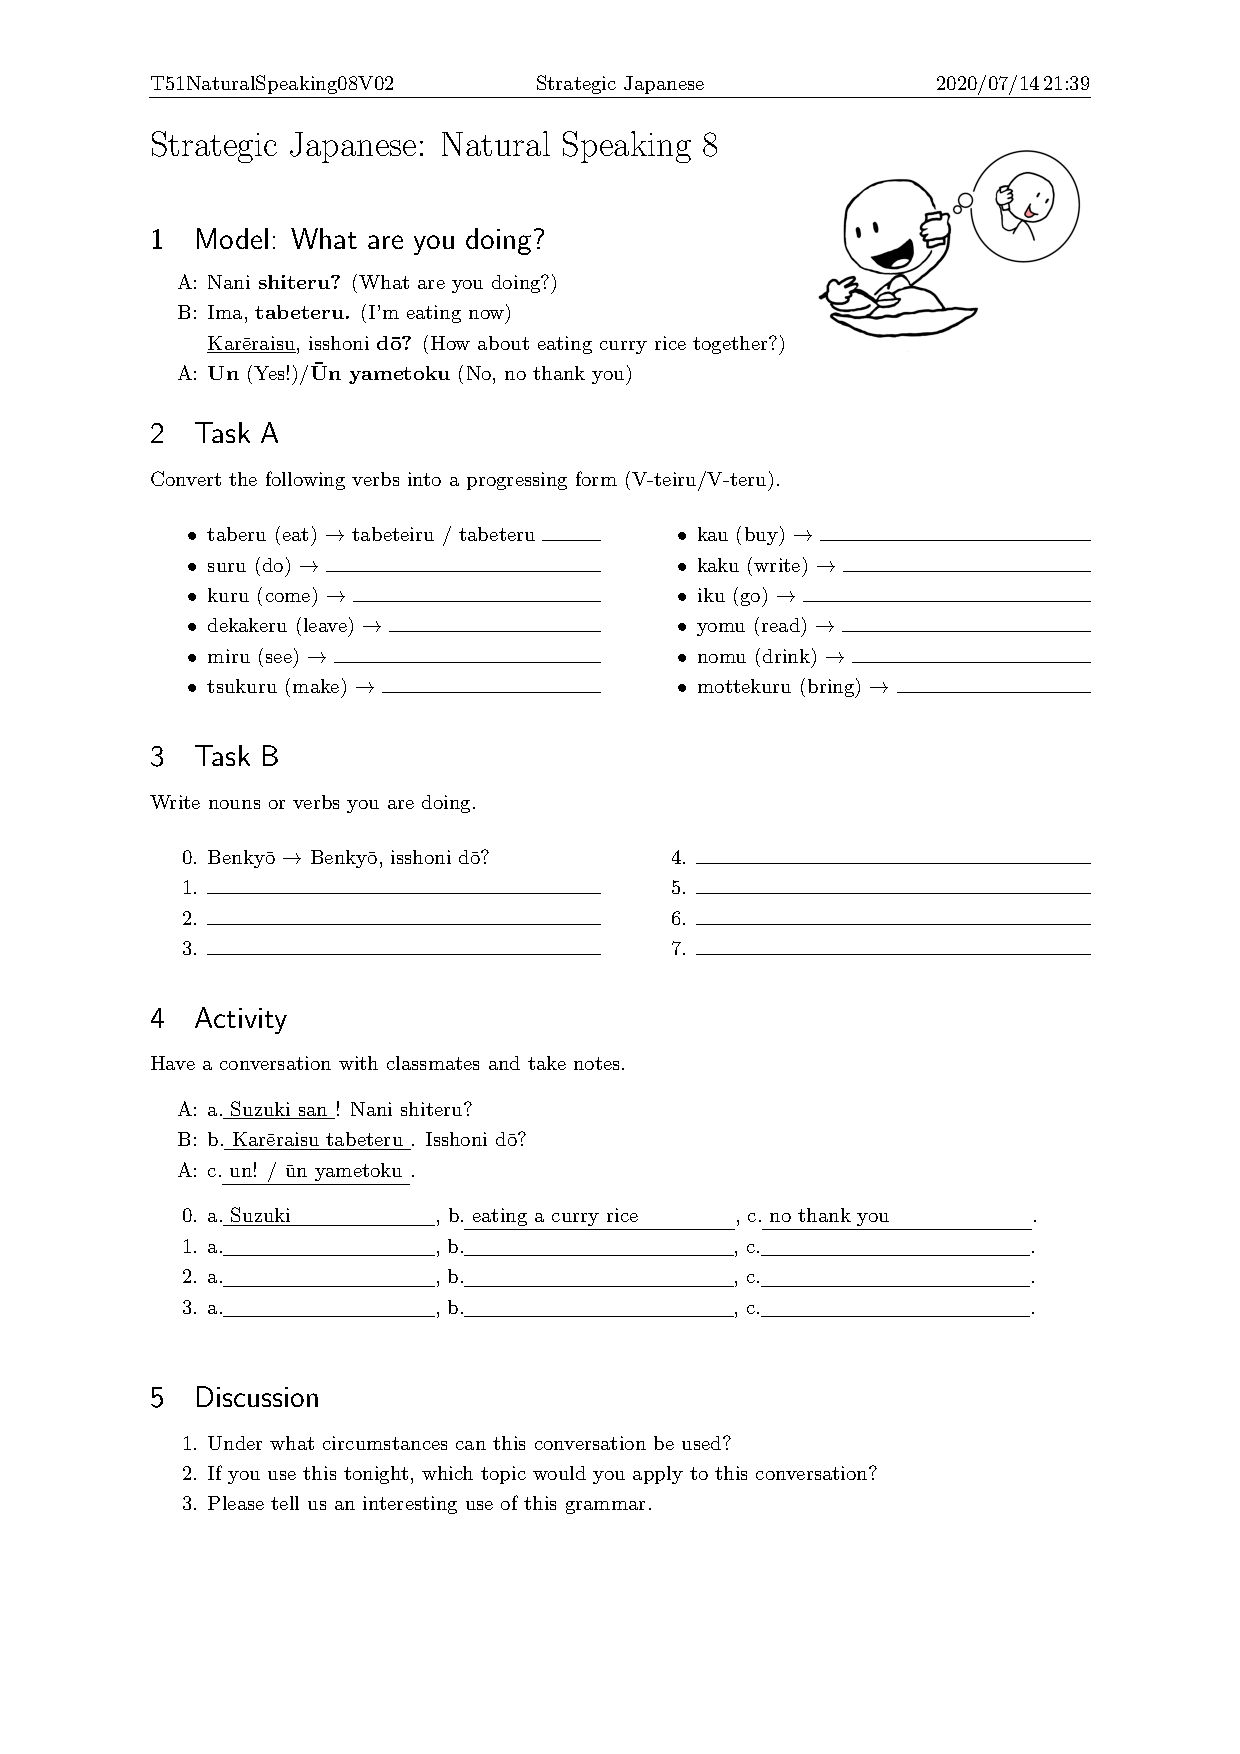
\includepdf[pages=-, scale=.86, trim=70 62 70 30, clip, offset=0mm -8.5mm, pagecommand={\thispagestyle{plain}}]{T51NaturalSpeaking08V02.pdf}

\ifEnglish
\section{Potential expression}
\else
\section{可能の表現}
\fi

%File: T51NaturalSpeaking09V02.pdf

\ifEnglish
\subsection{Model}
\else
\subsection{モデル}
\fi

\ifEnglish
You will learn a potential form of verb; {\it kore, dekiru\/} (can you do this?)
{\it sore nara\/} (if it is, I can do it)  would be convenient.
\else
可能形「これできる?」「それなら...」
\fi

\begin{toiquestion}
\ifEnglish
Discuss other situations in which {\it dekiru\/} can be used.
\else
「できる」が使える場面は以下の場面以外にどんな場面があるかを話し合いなさい。
\fi
\end{toiquestion}


\begin{itemize}
 \item[A:] kore {\bfseries dekiru?} (Can you do this?)
 \item[B:] uun, {\bfseries dekinai.} (No, I can't)
 \item[A:] j\=a, kore wa? (Well, how about this?)
 \item[B:] sore nara, {\bfseries dekiru.} (If it is, I can)
\end{itemize}

\begin{center}

\includegraphics[trim=110 20 100 40, clip, width=.18\hsize]{img/dekiru.png}
\end{center}

\begin{toianswer}
\ifEnglish
There are two cases: you can use it depending on your ability such as ``I can swim 100m'' or ``I can drive'';  you can use it depending on the situation such as ``I can swim in this river'' or ``I can't drive on this road.''
Discuss whether these usages are the same in your native language.
\else
たとえば「私は100m泳げる」「私は運転できる」のように自分の能力によって「できる」場合と、「この川では泳げる」「この道では運転できない」のように状況的に可能・不可能の場合がある。
あなたの母語でも、同じ使い方かどうかを話し合いなさい。
\fi
\end{toianswer}

\ifEnglish
\subsection{Task}
\else
\subsection{タスク}
\fi

\begin{toiquestion}
\ifEnglish
Convert the following verbs into a potential form (V-eru/V-rareru).
\else
動詞を可能形(V-eru/V-rareru)に変換する。
\fi
\end{toiquestion}

\begin{multicols}{2}
 \begin{enumerate}
 \setcounter{enumi}{-1}
 \item suru (do)        $\rightarrow$ {\bfseries dekiru}
 \item taberu (eat)     $\rightarrow$ taberareru / tabereru \hrulefill
 \item kuru (come)      $\rightarrow$ \hrulefill
 \item dekakeru (leave) $\rightarrow$ \hrulefill
 \item miru (see)       $\rightarrow$ {\bfseries mieru}
 \item kiku (hear)      $\rightarrow$ {\bfseries kikoeru}
 \item tsukuru (make)   $\rightarrow$ \hrulefill
 \item kau (buy)        $\rightarrow$ \hrulefill
 \item kaku (write)     $\rightarrow$ \hrulefill
 \item iku (go)         $\rightarrow$ \hrulefill
 \item yomu (read)      $\rightarrow$ \hrulefill
 \item nomu (drink)     $\rightarrow$ \hrulefill
 \end{enumerate}
\end{multicols}

\begin{toiquestion}
\ifEnglish
Write some items or skills you can/cannot do.
\else
自分ができる/できない項目やスキルをいくつか書け。
\fi
\end{toiquestion}

\begin{multicols}{2}
\begin{enumerate}
 \setcounter{enumi}{-1}
 \item \hrulefill\par
       \vspace{-1.2\baselineskip}\hspace{1em}{\bfseries ry\=ori}
       \vspace{.2\baselineskip}
 \item \hrulefill
 \item \hrulefill
 \item \hrulefill
 \item \hrulefill
 \item \hrulefill
\end{enumerate}
\end{multicols}

\ifEnglish
\subsection{Activity}
\else
\subsection{アクティビティ}
\fi

\begin{toiquestion}
\ifEnglish
Speak with your partners, and take notes.
\else
パートナーと話して、メモを取る。
\fi
\end{toiquestion}

\begin{itemize}
 \item[A:] a) Suzuki san b) {\bfseries ry\=ori dekiru?} (Suzukisan, can you cook?)
 \item[B:] uun, {\bfseries dekinai.} (No, I can't)
 \item[A:] j\=a, nani dekiru? (Well, what can you do?)
 \item[B:] c) {\bfseries piano hikeru/dekiru.} (I can play piano)
\end{itemize}

\begin{enumerate}
 \item[0.] \hrulefill\par
	   \vspace{-1.2\baselineskip}\hspace{.5em}a) Suzuki  \hspace{6.77em} b) ry\=ori dekinai \hspace{6.12em} c) piano hikeru
	   \vspace{.2\baselineskip}
 \item \hrulefill\par
       \vspace{-1.2\baselineskip}\hspace{.5em}a) \hspace{10em} b) \hspace{12em} c)
       \vspace{.2\baselineskip}
 \item \hrulefill\par
       \vspace{-1.2\baselineskip}\hspace{.5em}a) \hspace{10em} b) \hspace{12em} c)
       \vspace{.2\baselineskip}
 \item \hrulefill\par
       \vspace{-1.2\baselineskip}\hspace{.5em}a) \hspace{10em} b) \hspace{12em} c)
       \vspace{.2\baselineskip}
 \item \hrulefill\par
       \vspace{-1.2\baselineskip}\hspace{.5em}a) \hspace{10em} b) \hspace{12em} c)
       \vspace{.2\baselineskip}
 \item \hrulefill\par
       \vspace{-1.2\baselineskip}\hspace{.5em}a) \hspace{10em} b) \hspace{12em} c)
       \vspace{.2\baselineskip}
\end{enumerate}

\ifEnglish
\section{Discussion}
\else
\section{ディスカッション}
\fi

\begin{toiquestion}
\ifEnglish
Discuss how you can converse more fluently with your partners.
\else
もっと流暢に相手と会話がするにはどうすればよいかを話し合いなさい。
\fi
\end{toiquestion}
\begin{toianswer}
\ifEnglish
Be prepared intellectually rather than grammatically.
Think about and practice a few situations in which you will ask someone if it is possible.
It's good to refer to something, but it's easier to remember if you consider situations and prepare them by yourself.
\else
文法的な準備よりも知識的な準備をしておくこと。
誰かに可能かどうかを尋ねる場面をいくつか考えておいて、練習しておくこと。
何かを参考にするのもよいが、自分で考えて準備した方が記憶に残りやすい。
\fi
\end{toianswer}


%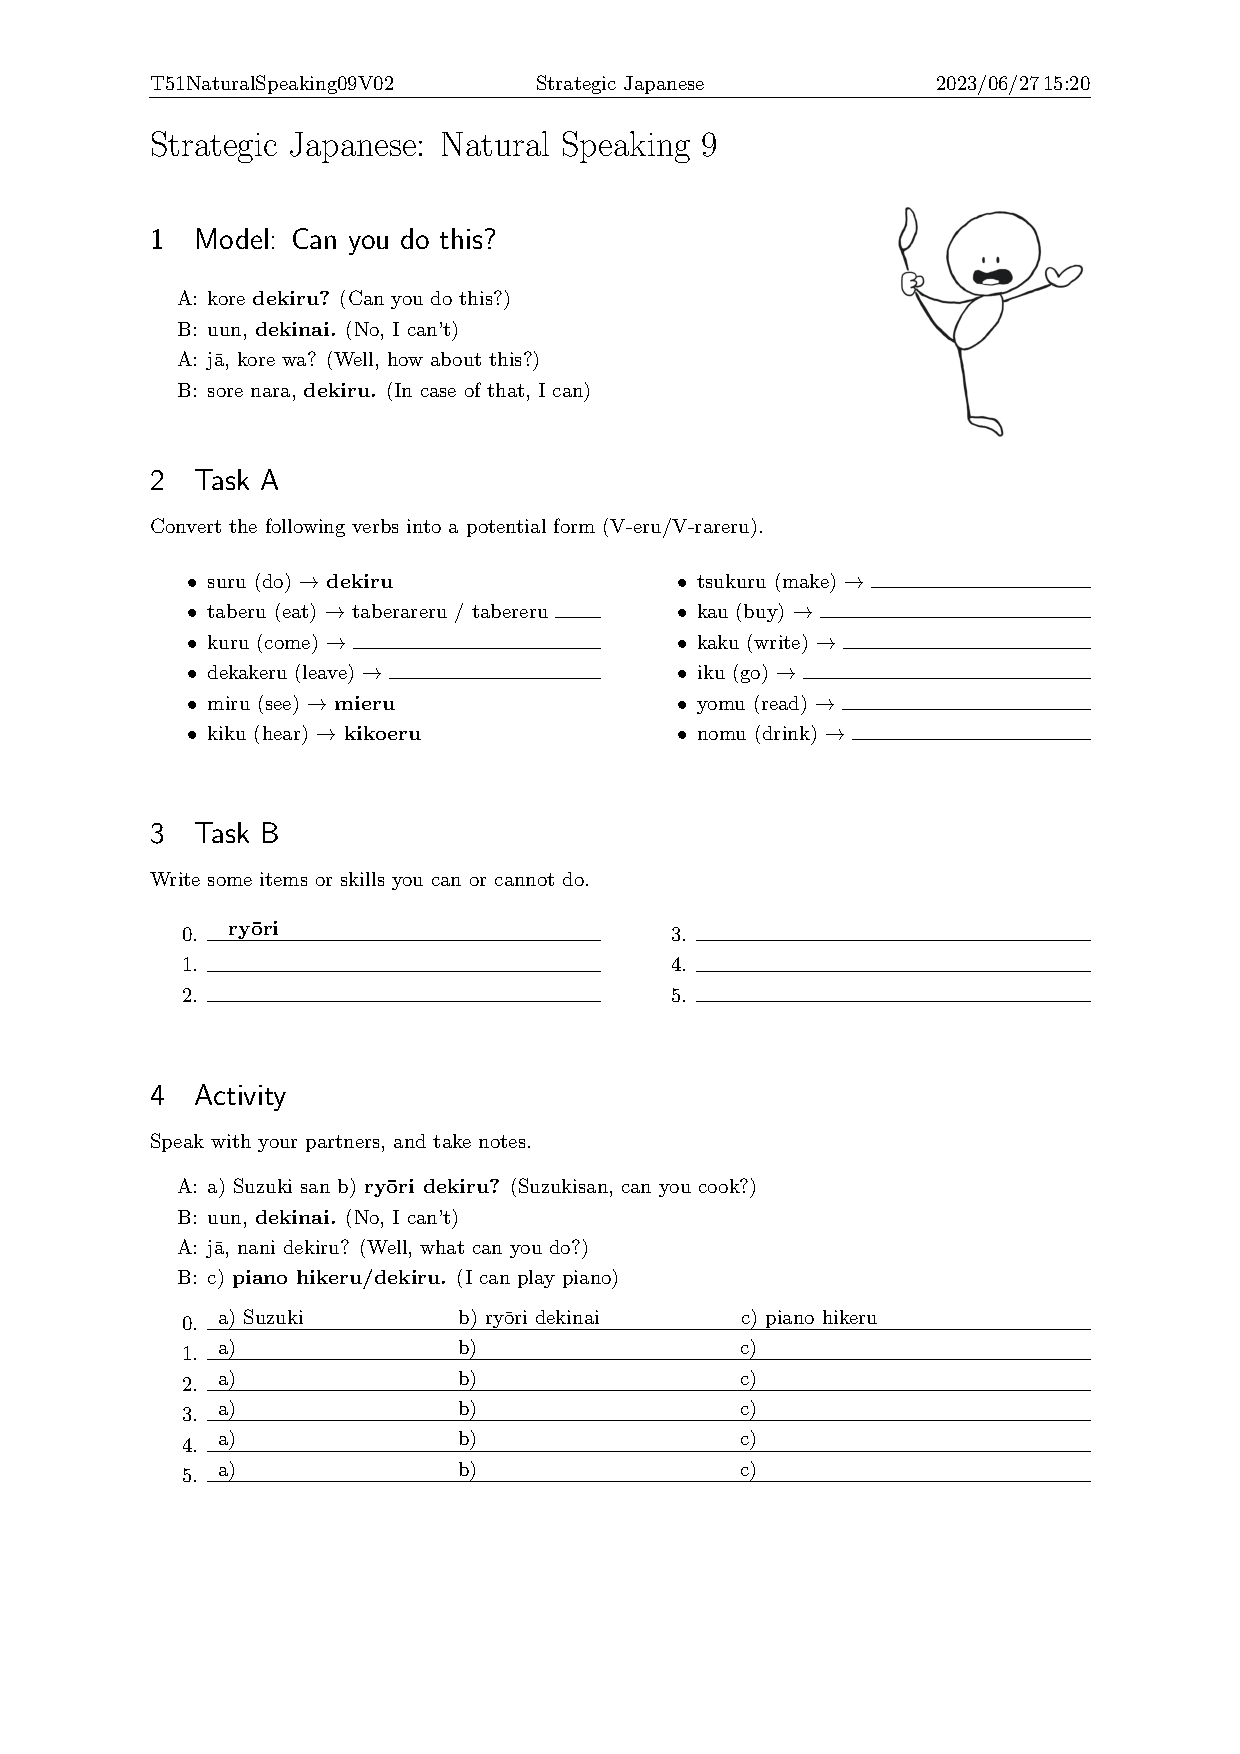
\includepdf[pages=-, scale=.86, trim=70 62 70 30, clip, offset=0mm -8.5mm, pagecommand={\thispagestyle{plain}}]{T51NaturalSpeaking09V02.pdf}

\fi%NATURALSPEAKINGPARTTWO


\ifNATURALSPEAKINGPARTTHREE
\ifEnglish
\chapter{Natural Speaking: Part 3} % 2022-08-24
\else
\chapter{自然に話すこと: Part 3}
\fi

\ifEnglish
  \section{Experiences}
\else
  \section{経験を話す}
\fi

%Natural Speaking 10 (New T51NaturalSpeaking10, Old File: T51Menu01): Using food menu, practice i-adjectives and V-ta koto ga aru.

%ビデオ「ハイ・ヌーン」を見るならば、内容的に重複するところがある。
%こちらはJC2の方にまわしたほうが良い。
%Natural Speaking 10は回数的には、JC2になる予定である。

\ifEnglish
\subsection{Japanese Food Menu}
\else
\subsection{日本食の品名}
\fi

\begin{toiquestion}
\ifEnglish
Figure\,\ref{fig:japanesefoodmenu} is a series of photographs of a typical Japanese b-class gourmet.
Discuss what the dish is and what it contains.
Discuss how many types of dishes can be classified.
\else
図\ref{fig:japanesefoodmenu}は典型的な日本のB級グルメの写真である。
どんな料理か、何が入っているかを話し合いなさい。
料理はいくつに分類できるかについても話し合いなさい。
\fi
\end{toiquestion}

\begin{figure}[htb]\centering\small
{\ttfamily\small
\begin{flushright}
a.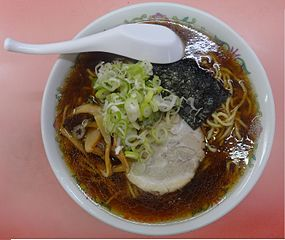
\includegraphics[trim=0 0 0 0, clip,     width=25mm, height=20mm]{img/shoyuramen.jpg}
b.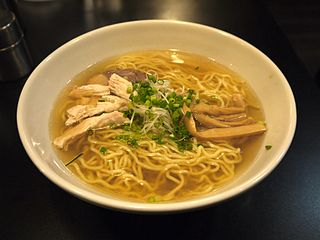
\includegraphics[trim=0 11 0 6, clip,    width=25mm, height=20mm]{img/shioramen.jpg}
c.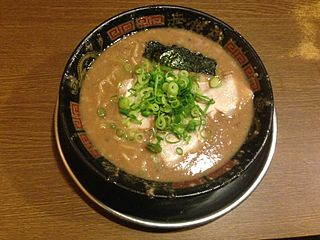
\includegraphics[trim=40 40 40 0, clip,  width=25mm, height=20mm]{img/tonkotsuramen.jpg}
d.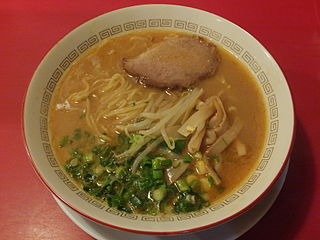
\includegraphics[trim=0 0 0 0, clip,     width=25mm, height=20mm]{img/misoramen1.jpg}

e.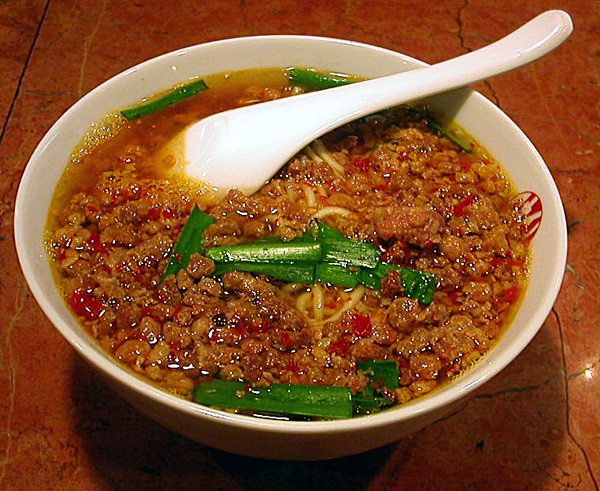
\includegraphics[trim=0 50 5 0, clip,    width=25mm, height=20mm]{img/CodazziTaiwanRamen.jpg}
f.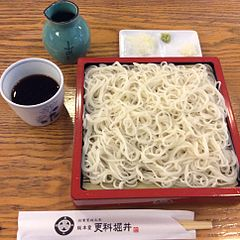
\includegraphics[trim=0 40 0 0, clip,    width=25mm, height=20mm]{img/zarusoba.jpg}
g.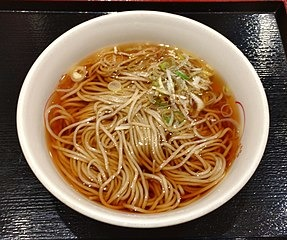
\includegraphics[trim=0 13 0 7, clip,    width=25mm, height=20mm]{img/kakesoba2.jpg}
h.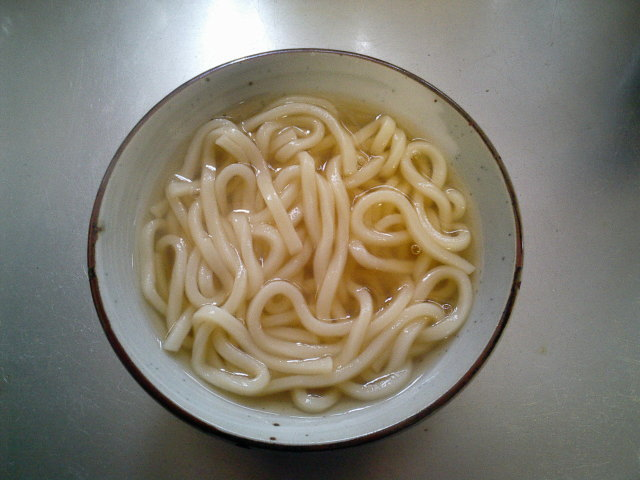
\includegraphics[trim=45 25 55 40, clip, width=25mm, height=20mm]{img/Kakeudon.jpg}

i.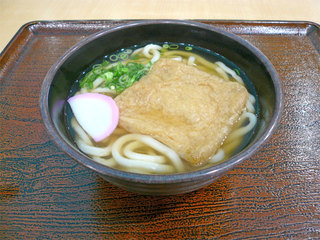
\includegraphics[trim=20 50 20 20, clip, width=25mm, height=20mm]{img/kitsuneudon.jpg}
j.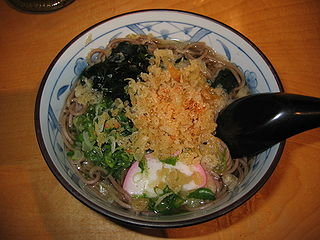
\includegraphics[trim=0 0 0 0, clip,     width=25mm, height=20mm]{img/tanukisoba.jpg}
k.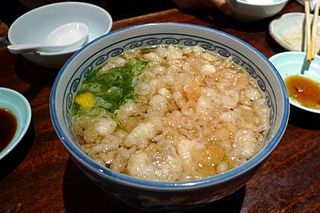
\includegraphics[trim=0 0 0 0, clip,     width=25mm, height=20mm]{img/tanukiudon.jpg}
l.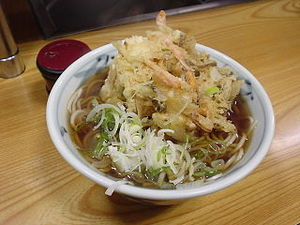
\includegraphics[trim=30 30 10 20, clip, width=25mm, height=20mm]{img/kakiagesoba.jpg}

m.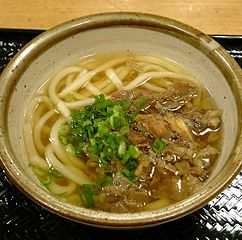
\includegraphics[trim=0 4 0 4, clip,     width=25mm, height=20mm]{img/nikuudon.jpg}
n.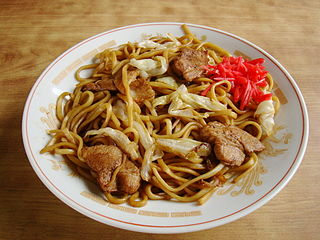
\includegraphics[trim=0 3 0 16, clip,    width=25mm, height=20mm]{img/yakisoba.JPG}
o.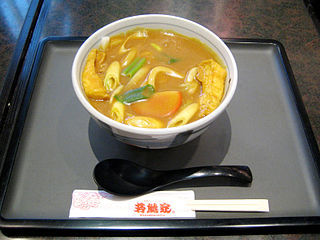
\includegraphics[trim=20 40 30 4, clip,  width=25mm, height=20mm]{img/curryudon.jpg}
p.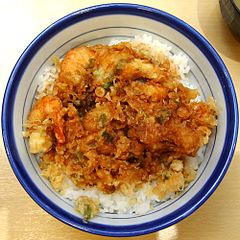
\includegraphics[trim=0 0 0 0, clip,     width=25mm, height=20mm]{img/kakiagedon.jpg}

q.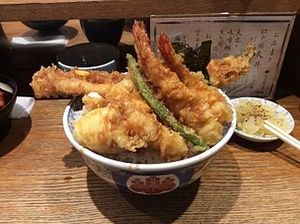
\includegraphics[trim=30 50 40 20, clip, width=25mm, height=20mm]{img/tendon.JPG}
r.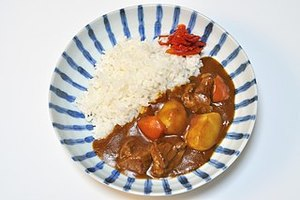
\includegraphics[trim=30 0 30 0, clip,   width=25mm, height=20mm]{img/curryrice.jpg}
s.\includegraphics[trim=0 20 0 20, clip,   width=25mm, height=20mm]{img/katsucurryrice.jpg}
t.\includegraphics[trim=0 0 0 0, clip,     width=25mm, height=20mm]{img/omurice3.jpg}
\end{flushright}
 }
\caption{Japanese food menu}
\label{fig:japanesefoodmenu}
\end{figure}

\begin{toianswer}
\begin{itemize}\small
 \item[{\ttfamily a.}] 醤油ラーメン Sh\=oyu R\=amen (Ramen noodles with soy source)
 \item[{\ttfamily b.}] 塩ラーメン Shio R\=amen (Ramen noodles with salty soup)
 \item[{\ttfamily c.}] とんこつラーメン Tonkotsu R\=amen (Ramen noodles with Pork Broth)
 \item[{\ttfamily d.}] 味噌ラーメン Miso R\=amen (Ramen noodles with miso soup)
 \item[{\ttfamily e.}] 激辛ラーメン Gekikara R\=amen (Spicy hot ramen noodles)
 \item[{\ttfamily f.}] ざるそば Zaru Soba (Soba noodles served on a bamboo draining basket)
 \item[{\ttfamily g.}] かけそば Kake Soba (Simple hot soba noodles)
 \item[{\ttfamily h.}] かけうどん Kake Udon (Simple hot udon noodles)
 \item[{\ttfamily i.}] きつねそば・うどん Kitsune Soba/Udon (Noodles topped with deep-fried tofu)
 \item[{\ttfamily j.}] たぬきそば Tanuki Soba (Soba noodles with crunchy bits of deep-fried dough)
 \item[{\ttfamily k.}] たぬきうどん Tanuki Udon (Udon noodles with crunchy bits of deep-fried dough)
 \item[{\ttfamily l.}] かきあげそば Kakiage Soba (Soba noodles topped with mixed vegetables tempura)
 \item[{\ttfamily m.}] 肉うどん Niku Udon (Udon noodles in a hot soup with beef)
 \item[{\ttfamily n.}] 焼きそば Yaki Soba (Fried noodle with vegetables and meat)
 \item[{\ttfamily o.}] カレーうどん Curry Udon (Udon noodles in a hot, thick curry soup)
 \item[{\ttfamily p.}] かきあげ丼 Kakiage Don (Rice bowl topped with mixed vegetables)
 \item[{\ttfamily q.}] 天丼 Tendon (Rice bowl topped with mixed vegetables and shrimp)
 \item[{\ttfamily r.}] カレーライス Curry Rice (Curry source over rice)
 \item[{\ttfamily s.}] カツカレーライス Katsu Curry Rice (Pork cutlet curry source over rice)
 \item[{\ttfamily t.}] オムライス Omu Rice (Pork cutlet curry over rice)
 \item Creative Commons License\footnote{Creative commons license by
       a. CCBY 多摩に暇人;
       b. CC継承4.0 Lombroso;
       %c. CC継承3.0非移植 Hykw-a4;
       c. CC継承4.0 博多からきた女;
       d. CC Lombroso;
       e. CC継承3.0非移植 小太刀;
       f. CC継承4.0国際 Edomura no Tokuzo;
       g. CC1.0 毒島みるく;
       h. GFDL;
       i. GFDL;
       j. CC継承2.0 Opponent;
       k. CC継承2.0 Ewan Munro;
       l. CC表示2.0 shibainu from Hatsudai, Shibuya, Tokyo;
       m. GFDL Hykw-a4; %nikuudon
       n. Public domain;
       o. Public domain Lombroso;
       p. CC表示2.0 chidorian;
       q. CC継承4.0国際 Edomura no Tokuzo;
       r. CC1.0 Ocdp;
       s. CC継承3.0非移植 Hykw-a4;
       %t. CC継承2.0 perago89; %360px-Omurice_by_perago89_in_Asakusa,_Tokyo.jpg
       t. CC継承2.0 hirotomo t from Japan; % convert 320px-オムライス_\(36248670142\).jpg omurice2.eps
     }
\end{itemize}
\end{toianswer}

\ifEnglish
\subsection{Task}
\else
\subsection{タスク}
\fi

\begin{toiquestion}
\ifEnglish
Ask each other and write down which you have ever eaten.
\else
経験の表現(〜たことがある)、食べ物に関する形容詞の練習。
\fi
\end{toiquestion}

\begin{itemize}
 % \item[A:] a. \underline{ Suzuki } san, nani taberu? \\\hspace{1em}(What are you going to eat?)
 \item[A:] \underline{ Suzuki } san, \underline{ kar\=e raisu } {\bfseries tabeta koto aru}? (Have you ever eaten kar\=e raisu?)
 \item[B:] \underline{ Aru (yes) / nai (no) / arimasu / arimasen }.
\end{itemize}

\begin{multicols}{2}
 \begin{enumerate}
 \setcounter{enumi}{-1}
  \item Curry rice \hrulefill
  \item \hrulefill
  \item \hrulefill
  \item \hrulefill
  \item \hrulefill
  \item \hrulefill
 \end{enumerate}
\end{multicols}

\begin{toianswer}
\ifEnglish
{\it V-ta koto ga aru\/} is an expression that expresses experience.
Replace {\it te\/} in the verb te-form with {\it ta\/} to form the verb ta-form.
\else
「~たことがある」は経験を表わす表現である。
動詞のテ形の「テ」を「タ」に置き換えて、動詞「~た」の形を作る。
\fi
\end{toianswer}

\begin{toiquestion}
\ifEnglish
Convert the following i-adjectives into the negative form.
\else
形容詞を否定形に変換する練習。
\fi
\end{toiquestion}

\begin{multicols}{2}
 \begin{enumerate}
  \setcounter{enumi}{-1}
  \item oisii? (tasty)   $\rightarrow$ \hrulefill
  \item amai? (sweet)    $\rightarrow$ \hrulefill
  \item karai? (spicy)   $\rightarrow$ \hrulefill
  \item atatakai? (warm) $\rightarrow$ \hrulefill
  \item tsumetai? (cold) $\rightarrow$ \hrulefill
  \item suppai? (sour)   $\rightarrow$ \hrulefill
  \item nigai? (bitter)  $\rightarrow$ \hrulefill
  \item atsui? (hot)     $\rightarrow$ \hrulefill
 \end{enumerate}
\end{multicols}

\begin{toianswer}
\ifEnglish
See \S\,\ref{gn:i-adj-past} for how to form the past tense of i-adjectives.
\else
イ形容詞の過去形の作り方は\S\,\ref{gn:i-adj-past}を参照する。
\fi
\end{toianswer}

\ifEnglish
\subsection{Activity}
\else
\subsection{アクティビティ}
\fi

\begin{toiquestion}
\ifEnglish
Ask your classmates what s/he will eat.
\else
クラスメートに何を食べるかを聞く。
おいしいかどうか意見を求められて、何かを言わなければならないとき、まあね、まあまあ、などと答える。
\fi
\end{toiquestion}

\begin{itemize}
 % \item[A:] a. \underline{ Suzuki } san, nani taberu? \\\hspace{1em}(What are you going to eat?)
 \item[A:] a. \underline{ Suzuki } san, nani taberu? (What are you going to eat?)
 \item[B:] b. \underline{ Kar\=e raisu }. (Curry rice.)
 \item[A:] Sore oishii? (Is that tasty?)
 \item[B:] c. \underline{ Un, oishiiyo. / ee, m\=ane. (so so) /}\\\hspace{1.1em}\underline{  \=un, shiranai (don't know) / m\=a, nantonaku (somehow seems good)}.
\end{itemize}

\begin{flushright}
\vspace{-6\baselineskip}
\includegraphics[trim=0 0 0 0, clip, angle=0, width=25mm]{img/Japanese-food-menu.png}
\vspace{2\baselineskip}
\end{flushright}

\begin{enumerate}
 \itemsep=4pt
 %\item[]\hspace{2em}Suzuki san\hspace{6.8em}Curry rice\hspace{7em}Ee, m\=ane\\[-20pt]
 \item[0.] a. \underline{\hspace{10em}} b. \underline{\hspace{10em}}  c. \hrulefill.
 \item a. \underline{\hspace{10em}} b. \underline{\hspace{10em}}  c. \hrulefill.
 \item a. \underline{\hspace{10em}} b. \underline{\hspace{10em}}  c. \hrulefill.
 \item a. \underline{\hspace{10em}} b. \underline{\hspace{10em}}  c. \hrulefill.
 \item a. \underline{\hspace{10em}} b. \underline{\hspace{10em}}  c. \hrulefill.
 \item a. \underline{\hspace{10em}} b. \underline{\hspace{10em}}  c. \hrulefill.
 \item a. \underline{\hspace{10em}} b. \underline{\hspace{10em}}  c. \hrulefill.
\end{enumerate}

\begin{toianswer}
\ifEnglish
If you think about it a little, you'll understand that there aren't many situations where you can clearly say ``it's not delicious.''
\else
はっきりと「おいしくない」という場面は、多くないことは少し考えればわかるだろう。
\fi
\end{toianswer}


\ifEnglish
\subsection{Discussion}
\else
\subsection{ディスカッション}
\fi

\begin{toiquestion}
\ifEnglish
What is important to speak naturally?
\else
自然に話すには何が重要か。
\fi
\end{toiquestion}
\begin{toiquestion}
\ifEnglish
What kinds of words do you need to improve my conversations?
\else
会話を上達させるためにはどんな単語が必要ですか。
\fi
\end{toiquestion}
\begin{toiquestion}
\ifEnglish
What kinds of techniques can you add to make your speech more natural?
\else
より自然に話すためには、どんなテクニックをプラスすればいいのでしょうか?
\fi
\end{toiquestion}

%\includepdf[pages=-, scale=.86, trim=70 62 70 30, clip, offset=0mm -8.5mm, pagecommand={\thispagestyle{plain}}]{T51NaturalSpeaking10V02.pdf}
%\includepdf[pages=-, scale=.86, trim=70 62 70 30, clip, offset=0mm -8.5mm, pagecommand={\thispagestyle{plain}}]{T51Menu02.pdf}


\ifEnglish % 2022-08-27
\section{Tried to do it, but..}
\else
\section{〜ようと思ったけど}
\fi

%Natural Speaking 11 (old T51Verb01.pdf) 意向形の練習。

%\ifEnglish
%  Natural Use of Verbs part 1: ..y\=oto omotta kedo.
%\else
%  自然な動詞の使い方: 「〜ようと思ったけど」
%\fi

\ifEnglish
\subsection{Model}
\else
\subsection{モデル}
\fi

\begin{itemize}
 \item[A:] kinou itta? (Did you go there yesterday?)
 \item[B:] {\bfseries ikou to omotta} kedo... (I tried to go there, but..)
 \item[A:] dou shita no? (What happened?)
 \item[B:] ikanakatta (I did not go there.)
 \item[A:] doushite? (Why?)
 \item[B:] chotto isogashikatta (I was busy) / wasureta (I forgot)
\end{itemize}

%%\ifILLUST
%\vspace*{-10\baselineskip}
%\begin{flushright}
%\includegraphics[trim=50 80 150 50, clip, width=.3\hsize]{komattakao.pdf}
%%\fbox{\includegraphics[trim=50 80 130 80, clip, width=.3\hsize]{../pictures/yooto.png}}
\begin{center}
  \fbox{\includegraphics[trim=40 100 110 80, clip, width=.3\hsize]{img/yooto.png}}
\end{center}
%\end{flushright}
%\vspace*{04\baselineskip}
%%\fi%ILLUST

\ifEnglish
\subsection{Task}
\else
\subsection{タスク}
\fi

\begin{toiquestion}
\ifEnglish
Convert the following verbs into past tense and volitional form.
GN(grammar notes) or Verb Cheet Sheet are available.
\else
次の動詞を過去形と動詞の形に変換せよ。
GN(文法ノート)や動詞のチートシートが用意されている。
\fi
\end{toiquestion}

\begin{multicols}{2}
\begin{enumerate}
\setcounter{enumi}{-1}
 \item tsukuru (make) $\rightarrow$ tsukutta, tsukur\=o \hrulefill
 \item suru (do)     $\rightarrow$ \hrulefill
 \item kuru (come)   $\rightarrow$ \hrulefill
 \item hairu (enter) $\rightarrow$\hrulefill
 \item deru (leave)  $\rightarrow$ \hrulefill
 \item dekakeru (leave) $\rightarrow$ \hrulefill
 \item yomu (read)   $\rightarrow$ \hrulefill
 \item kaku (write)  $\rightarrow$ \hrulefill
 \item iku (go)   $\rightarrow$ \hrulefill
 \item asobu (play)   $\rightarrow$ \hrulefill
 \item taberu (eat)   $\rightarrow$ \hrulefill
 \item nomu (drink)   $\rightarrow$ \hrulefill
 \item kau (buy)   $\rightarrow$ \hrulefill
 \item miru (see)   $\rightarrow$ \hrulefill
 \item mottekuru (bring)   $\rightarrow$ \hrulefill
 \item kureru (give me)   $\rightarrow$ \hrulefill
\end{enumerate}
\end{multicols}

\begin{toianswer}
\ifEnglish
As usual, we'll go through 3G, 2G, and then 1G.
{\it Suru\/} and {\it kuru\/} are converted such as:
3G {\bfseries suru} $\rightarrow$ {\bfseries shiyou}, {\bfseries kuru}    $\rightarrow$ {\bfseries koyou}.
2G replaces {\it ru\/} at the end of verbs in the dictionary form with {\it you\/} such as:
2G tabe{\bfseries ru}  $\rightarrow$ tabe{\bfseries you}.
1G replaces {\it u\/} with {\it ou\/} at the end of verbs in dictionary form such as:
1G tsukur{\bfseries u} $\rightarrow$ tsukur{\bfseries ou}.
\else
いつものように、3G, 2G, そして、1Gの順で説明する。
「する」と「くる」は次のように変換する。
 3G {\bfseries suru} $\rightarrow$ {\bfseries shiyou}, {\bfseries kuru}    $\rightarrow$ {\bfseries koyou}
2Gは辞書形の動詞語末のruをyouに置き換える。
 2G tabe{\bfseries ru}  $\rightarrow$ tabe{\bfseries you};
1Gは辞書形の動詞語末のuをouに置き換える。
 1G tsukur{\bfseries u} $\rightarrow$ tsukur{\bfseries ou},
   ka{\bfseries u} $\rightarrow$ ka{\bfseries ou}.
\fi
\end{toianswer}

\ifEnglish
\subsection{Activity}
\else
\subsection{アクティビティ}
\fi

\begin{toiquestion}
\ifEnglish
Have a conversation and take notes.
\else
会話をして、ノートを取りなさい。
\fi
\end{toiquestion}

\begin{itemize}
 \item[A:] a.\underline{a. Suzuki \hspace{1zw}} san! doushita no?
 \item[B:] b.\underline{b. Ikou \hspace{1zw}} to omotta kedo...
 \item[A:] doushita no?
 \item[B:] \underline{ ikanakatta \hspace{1zw}}.
 \item[A:] doushite?
 \item[B:] c.\underline{ chotto isogashikatta.\hspace{1zw}}
\end{itemize}

\begin{enumerate}
 \setcounter{enumi}{-1}
 \item a.\underline{ Suzuki \hspace{6.5em}}, b.\underline{ go (ikou) \hspace{7.45em}}, c.\underline{ isogashikatta \hspace{1.2em}}.
 \item a.\underline{\hspace{10em}}, b.\underline{\hspace{9em}}, c.\hrulefill.
 \item a.\underline{\hspace{10em}}, b.\underline{\hspace{9em}}, c.\hrulefill.
 \item a.\underline{\hspace{10em}}, b.\underline{\hspace{9em}}, c.\hrulefill.
 \item a.\underline{\hspace{10em}}, b.\underline{\hspace{9em}}, c.\hrulefill.
 \item a.\underline{\hspace{10em}}, b.\underline{\hspace{9em}}, c.\hrulefill.
 \item a.\underline{\hspace{10em}}, b.\underline{\hspace{9em}}, c.\hrulefill.
\end{enumerate}

\ifEnglish
\subsection{Discussion}
\else
\subsection{ディスカッション}
\fi

\begin{toiquestion}
\ifEnglish
What kind of verbs did you want to use more?
\else
もっと使ってみたいと思ったのはどんな動詞か?
\fi
\end{toiquestion}
\begin{toianswer}
\ifEnglish
It is good to consider not only the verb, but also the reason.
\else
動詞だけでなく、理由もいっしょに考えておくとよい。
\fi
\end{toianswer}

\begin{toiquestion}
\ifEnglish
In which timings did you want to use those verbs?
\else
その動詞をどのタイミングで使いたいと思ったか?
\fi
\end{toiquestion}
\begin{toianswer}
\ifEnglish
It can be used when for some reason you cannot do it.
Of course, the reason is that you don't want to do it.
\else
何か理由があって、それができなかったときに使える。
もちろん、やりたくないというのも理由である。
\fi
\end{toianswer}


\begin{toiquestion}
\ifEnglish
What kind of techniques do you need to use when you speak with your partners more fluently?
\else
流暢に会話するためには、どのようなテクニックが必要か?
\fi
\end{toiquestion}
\begin{toianswer}
\ifEnglish
Respond immediately when someone asks you a question.
If you don't know what you want to say, just say {\it eeto\/} or {\it sonou\/} and don't keep silence.
\else
相手に聞かれたらすぐに返答すること。
言いたいことがわからないときは、「えーと」「そのう」など言っておき、黙ったままでいないこと。
\fi
\end{toianswer}


%\includepdf[pages=-, scale=.86, trim=70 62 70 30, clip, offset=0mm -8.5mm, pagecommand={\thispagestyle{plain}}]{T51Verb01.pdf}
%\includepdf[pages=-, scale=.86, trim=70 62 70 30, clip, offset=0mm -8.5mm, pagecommand={\thispagestyle{plain}}]{T51NaturalSpeaking11V02OLDVerb01.pdf}


\ifEnglish
  \section{Request/offer advice}
\else
  \section{アドバイスを求める・する}
\fi

\ifEnglish
\subsection{Model}
\else
\subsection{モデル}
\fi

\begin{toiquestion}
\ifEnglish
Learn expressions for asking for advice.
Read the following model with the expression {\it ..ba ii\/}.
\else
アドバイスを求める表現について学ぶ。
「~ばいい」の表現に注目して次のモデルを読みなさい。
\fi
\end{toiquestion}

\begin{itemize}
 \item[A:] \underline{Happyou}, dou {\bfseries sureba ii?} (My presentation, how should I do it?)
 \item[B:] \underline{Senpai ni} {\bfseries kikeba ii} yo! (Asking your senior would be a good idea!)
 \item[C:] {\bfseries Dousureba ii darounee}... (How can you do for it...I don't know either!)
\end{itemize}

\begin{toianswer}
\ifEnglish
The expression {\it ...ba ii\/} is certainly a conditional expression, but the usage here is an expression when giving advice to someone.
\else
「~ばいい」の表現は確かに条件の表現だが、ここでの使い方は誰かにアドバイスするときの表現である。
\fi
\end{toianswer}


\ifEnglish
\subsection{Task}
\else
\subsection{タスク}
\fi

\begin{toiquestion}
\ifEnglish
Convert the following verbs into conditional form.
\else
動詞を条件形に変換する。
\fi
\end{toiquestion}

\begin{multicols}{2}
\begin{enumerate}
 \setcounter{enumi}{-1}
 \item suru (do) $\rightarrow$ sureba ii \hrulefill
 \item kuru (come)   $\rightarrow$ \hrulefill
 \item taberu (eat)   $\rightarrow$ \hrulefill
 \item dekakeru (leave) $\rightarrow$ \hrulefill
 \item miru (see)  $\rightarrow$ \hrulefill
 \item tsukuru (make) $\rightarrow$ \hrulefill
 \item kau (buy)   $\rightarrow$ \hrulefill
 \item kaku (write)  $\rightarrow$ \hrulefill
 \item iku (go)   $\rightarrow$ \hrulefill
 \item yomu (read)   $\rightarrow$ \hrulefill
 \item nomu (drink)   $\rightarrow$ \hrulefill
 \item mottekuru (bring)   $\rightarrow$ \hrulefill
 \end{enumerate}
\end{multicols}

\begin{toianswer}
\ifEnglish
See grammar notes for conditional expressions and how to create conditional forms.
\else
条件の表現、条件形の作り方はGrammar notesを参照のこと。
\fi
\end{toianswer}

\begin{toiquestion}
\ifEnglish
Write down what you don't know how to deal with.
\else
どうしたらいいかわからないことを書き出す。
\fi
\end{toiquestion}

\begin{multicols}{2}
\begin{enumerate}
 \setcounter{enumi}{-1}
 \item \hrulefill
 \vspace{-1.1\baselineskip}
 \item[] \ \ happyou
 \item \hrulefill
 \item \hrulefill
 \item \hrulefill
 \item \hrulefill
 \item \hrulefill
 \item \hrulefill
 \item \hrulefill
\end{enumerate}
\end{multicols}

\begin{toianswer}
\ifEnglish
How to write documents, how to cook, and how to make friends are also good.
If you know how to do them, think about how you would advise them.
\else
書類の書き方、料理の作り方、友達の作り方などもよい。
もし、それらの方法を知っている場合には、どうアドバイスするかを考えてみよう。
\fi
\end{toianswer}

\ifEnglish
\subsection{Activity}
\else
\subsection{アクティビティ}
\fi
\begin{toiquestion}
\ifEnglish
Have a conversation and take notes.
\else
会話をして、メモを取る。
\fi
\end{toiquestion}

\begin{itemize}
 \item[A:] a.\underline{ Suzuki } san! b.\underline{ Happyou }, dou sureba ii?
 \item[B:] c.\underline{ Senpai ni kikeba ii} yo!
\end{itemize}

\begin{enumerate}
 \setcounter{enumi}{-1}
 \item a.\underline{ Suzuki \hspace{6.1zw}}, b.\underline{ happyo\hspace{6.2zw}}, c.\underline{ senpai ni kikeba ii\hspace{4zw}}.
 \item a.\underline{\hspace{10zw}}, b.\underline{\hspace{10zw}}, c.\underline{\hspace{13zw}}.
 \item a.\underline{\hspace{10zw}}, b.\underline{\hspace{10zw}}, c.\underline{\hspace{13zw}}.
 \item a.\underline{\hspace{10zw}}, b.\underline{\hspace{10zw}}, c.\underline{\hspace{13zw}}.
\end{enumerate}

\begin{toianswer}
\ifEnglish
If you don't know, answer {\it watashi mo wakaranai\/} (I don't know either).
{\it watashi mo wakaranai kedo, issho ni kangaemashou\/} (I don't know either. But let's check it out together).
{\it isshoni shirabemashou\/} (let's look it up together) or {\it toshokan he itte mimashou\/} (let's go to the library) are also good.
\else
わからないときは、「私もわからない」と答えよう。
「私もわからない。いっしょに考えましょう」というのもよい。
「いっしょに調べましょう」「図書館へ行ってみましょう」などもよい。
\fi
\end{toianswer}

\ifEnglish
\subsection{Discussion}
\else
\subsection{ディスカッション}
\fi

\begin{toiquestion}
\ifEnglish
What kind of conjugation do you use for {\it ..ba\/} form?
\else
「~ば」の形はどのような活用をする?
\fi
\end{toiquestion}
\begin{toianswer}
\ifEnglish
3G is {\it suru\/} $\rightarrow$ {\it sureba\/}, {\it kuru\/} $\rightarrow$ {\it kureba\/}.
2G is {\it ..ru\/} $\rightarrow$ {\it ..reba\/}, for example {\it miru\/} $\rightarrow$ {\it mireba\/}, {\it taberu\/} $\rightarrow$ {\it tabereba\/}.
1G is {\it ...u\/} $\rightarrow$ {\it ...eru\/}, for example {\it kaku\/} $\rightarrow$ {\it kakeba\/}, {\it yomu\/} $\rightarrow$ {\it yomeba\/}.
\else
3Gは「する」$\rightarrow$「すれば」、「くる」$\rightarrow$「くれば」。
2Gは「る」$\rightarrow$「れば」、たとえば「見る」$\rightarrow$「見れば」、「食べる」$\rightarrow$「食べれば」。
1Gは「u」$\rightarrow$「eば」、たとえば「書く」$\rightarrow$「書けば」、「読む」$\rightarrow$「読めば」。
\fi
\label{v-ba}
\end{toianswer}

\begin{toiquestion}
\ifEnglish
When are you going to use this expression?
\else
いつこの表現を使うか。
\fi
\end{toiquestion}
\begin{toianswer}
\ifEnglish
It can also be used when giving advice to someone.
In addition, although you are not very confident, you can use it like ``I wonder if I/we should do this'' when stating an idea.
\else
誰かにアドバイスするときにも使える。
その他、あまり自信はないが、何かアイデアを述べるとき、「こうすればいいかなぁ」のように使える。
\fi
\end{toianswer}

%\includepdf[pages=-, scale=.86, trim=70 62 70 30, clip, offset=0mm -8.5mm, pagecommand={\thispagestyle{plain}}]{T51NaturalSpeaking12Verb02.pdf}
%\includepdf[pages=-, scale=.86, trim=70 62 70 30, clip, offset=0mm -8.5mm, pagecommand={\thispagestyle{plain}}]{T51Verb02.pdf}

\ifEnglish % 2022-08-28
  \section{Expressing the feeling of a regret}
\else
  \section{後悔の念}
\fi

\ifEnglish
\subsection{Model}
\else
\subsection{モデル}
\fi

\begin{toiquestion}
\ifEnglish
Learn {\it ..ba yokatta\/} (I should have done) as a way to use natural verbs.
Practice expressing your impressions using past tense i-adjectives such as {\it omoshirokatta\/} (it was funny/interesting) and {\it tanoshikatta \/} (it was fun).
\else
自然な動詞の使い方として、「すればよかった」を学ぶ。
「おもしろかった」「たのしかった」などイ形容詞過去形を使って、感想を述べる練習をする。
\fi
\end{toiquestion}

\begin{itemize}
 \item[A:] Kinou no paatii, \underline{tanoshikatta!} (The party in yesterday was fun!)
 \item[B:] Aa, {\bfseries ikeba yokatta!} (I should've been there!)
 \item[A:] Sou! {\bfseries ikeba yokatta noni!} (Sorry, you should've been there!)
 \item[B:] Honto! {\bfseries zannen!} (True! I missed a chance!)
\end{itemize}

\begin{toianswer}
\ifEnglish
It's common to regret things you didn't do in the past, but few people say it.
I guess the reason why it is possible that the form of expression is difficult or why there are not many opportunities to say it.
However, telling someone that you regret it might give you a chance next time.
\else
過去しなかったことを後悔することはよくあるが、それを言う人は少ない。
理由はよくわからないが、表現の形式が難しかったり、言う機会があまり多くないことなどが考えられる。
しかし、後悔していることを伝えることは、次回、誰かがチャンスをくれるかもしれない。
\fi
\end{toianswer}

\ifEnglish
\subsection{Task}
\else
\subsection{タスク}
\fi

\begin{toiquestion}
\ifEnglish
Convert the following verbs into conditional form.
\else
動詞を条件形に書き換えよ。
\fi
\end{toiquestion}

\begin{multicols}{2}
 \begin{itemize}
 \setcounter{enumi}{-1}
 \item suru (do) $\rightarrow$ sureba yokatta \hrulefill
 \item kuru (come)   $\rightarrow$ \hrulefill
 \item taberu (eat)   $\rightarrow$ \hrulefill
 \item dekakeru (leave) $\rightarrow$ \hrulefill
 \item miru (see)  $\rightarrow$ \hrulefill
 \item tsukuru (make) $\rightarrow$ \hrulefill
 \item kau (buy)   $\rightarrow$ \hrulefill
 \item kaku (write)  $\rightarrow$ \hrulefill
 \item iku (go)   $\rightarrow$ \hrulefill
 \item yomu (read)   $\rightarrow$ \hrulefill
 \item nomu (drink)   $\rightarrow$ \hrulefill
 \item mottekuru (bring)   $\rightarrow$ \hrulefill
 \end{itemize}
\end{multicols}

\begin{toianswer}
\ifEnglish
See \S\,\ref{v-ba} for how to form the conditional form of verbs.
\else
動詞の条件形の作り方は、\S\,\ref{v-ba}を参照のこと。
\fi
\end{toianswer}

\begin{toiquestion}
\ifEnglish
Write down event names with your impression which you attended or things you did recently.
\else
参加したイベントや、最近行ったことなど、印象に残っているイベント名を書いてみよ。
\fi
\end{toiquestion}

\begin{multicols}{2}
\begin{enumerate}
 \setcounter{enumi}{-1}
 \item \hrulefill
 \vspace{-1.1\baselineskip}
 \item[]  party, fun/tanoshikatta
 \item \hrulefill
 \item \hrulefill
 \item \hrulefill
 \item \hrulefill
 \item \hrulefill
 \item \hrulefill
 \item \hrulefill
\end{enumerate}
\end{multicols}

\begin{toianswer}
\ifEnglish
You should be able to use most adjectives.
In the case of Japanese, choose i-adjectives and practice them in the past tense.
\else
だいたいの形容詞が使えるはずだ。
日本語の場合はイ形容詞を選んで過去形にして練習しておく。
\fi
\end{toianswer}

\ifEnglish
\subsection{Activity}
\else
\subsection{アクティビティ}
\fi

\begin{toiquestion}
\ifEnglish
Have a conversation and take notes.
\else
会話をして、メモを取る。
\fi
\end{toiquestion}

\begin{itemize}
 \item[A:] Kinou no a.\underline{ eiga }, b.\underline{ omoshirokatta! }
 \item[B:] c.\underline{ Ikeba yokatta } yo!
 \item[A:] Sou! c.\underline{ ikeba yokatta } noni!
 \item[B:] Ah, zannen!
\end{itemize}

\begin{enumerate}
 \setcounter{enumi}{-1}
 \item a.\underline{ Eiga\hspace{8.6zw}}, b.\underline{ omoshirokatta \hspace{3.4zw}}, c.\underline{ ikeba yokatta\hspace{3.4zw}}.
 \item a.\underline{\hspace{11zw}}, b.\underline{\hspace{11zw}}, c.\underline{\hspace{10zw}}.
 \item a.\underline{\hspace{11zw}}, b.\underline{\hspace{11zw}}, c.\underline{\hspace{10zw}}.
 \item a.\underline{\hspace{11zw}}, b.\underline{\hspace{11zw}}, c.\underline{\hspace{10zw}}.
\end{enumerate}

\begin{toianswer}
\ifEnglish
The word {\it noni\/} expresses regret.
Instead of saying {\it zannen\/} (I'm sorry), you can repeat the same words as {\it ikeba yokattane\/} (Yes, you should've gone there).
{\it Ja, jikai\/} (Well, next time), {\it ja, tsugi wa zehi\/} (well, next time definitely) are also good.
Discuss what kind of answers there are otherwise.
\else
「のに」ということばは残念な気持ちを表わす。
「残念」という以外にも、「行けばよかったね」と同じことばを繰り返してもよい。
「じゃ、次回」「じゃ、次は是非」という返答もよい。
それに類する回答にどんなものがあるかを話し合いなさい。
\fi
\end{toianswer}

\ifEnglish
\subsection{Discussion}
\else
\subsection{ディスカッション}
\fi

\begin{toiquestion}
\ifEnglish
What kind of conjugation do you use for v-ba form?
\else
動詞+「ば」の形はどのような活用をするか?
\fi
\end{toiquestion}
\begin{toianswer}
\ifEnglish
See \S\,\ref{v-ba} for how to form the conditional form of verbs.
\else
動詞の条件形の作り方は、\S\,\ref{v-ba}を参照のこと。
\fi
\end{toianswer}

\begin{toiquestion}
\ifEnglish
Have you ever missed an opportunity?
If so, please share your experience.
If not, listen to the experience and respond with {\it ..ba yokattane\/}.
\else
あなたは今迄に「チャンスを逃した」経験はあるか。
もし、あれば、そのときの経験を共有しなさい。
もし、なければ、経験を聞いて、「~ばよかったね」と反応しなさい。
\fi
\end{toiquestion}

\begin{toiquestion}
\ifEnglish
Could you have conversations with your partners more fluently?
\else
パートナーとの会話がより流暢にできるようになったかどうか話し合え?
\fi
\end{toiquestion}
\begin{toianswer}
\ifEnglish
We have learned that it is important to react immediately so far.
When you can't respond, just say something by saying {\it eeto\/}, {\it anou\/}, etc.
When you really have nothing else to say, look at the eyes of your lister and just nod.
Either way, you must let them know you are listening.
If you don't, you're ignoring the person you are now communicating with.
This must be avoided at all costs.
\else
ここまでに「すぐ反応する」のが重要だと説明した。
反応できないときには、「ええと」「あのう」などを言ってとにかく「何かを言う」こと。
他に本当に何も言えなかったときには、相手の目を見て「うなづく」こと。
いずれにしても、相手のことを聞いていることを伝えなければならない。
そうしなければ、相手を無視していることになる。
これは絶対に避けなければならない。
\fi
\end{toianswer}

%\includepdf[pages=-, scale=.86, trim=70 62 70 30, clip, offset=0mm -8.5mm, pagecommand={\thispagestyle{plain}}]{T51NaturalSpeaking13Verb03.pdf}
%\includepdf[pages=-, scale=.86, trim=70 62 70 30, clip, offset=0mm -8.5mm, pagecommand={\thispagestyle{plain}}]{T51Verb03.pdf}

\ifEnglish
\section{Describe several reasons}
\else
\section{理由を並べて言う}
\fi

%File: T51Discourse01.pdf

\ifEnglish
\subsection{Model}
\else
\subsection{モデル}
\fi

\begin{toiquestion}
\ifEnglish
To describe several reasons, you will use a construction of {\it ...shi, ...shi, ...\/}.
\else
理由を並べて言うときは、「...し、...し、...」の構文を使う。
\fi
\end{toiquestion}

\begin{itemize}
\item[A:] Doushite \underline{pa-thi- ni ikanai n desuka}? (why won't you go to the party?)
\item[B:] Anou, okane ga nai {\bfseries shi}, shukudai ga aru {\bfseries shi}.. (well, because I have no money, and I have homework...)
\item[A:] Soudesuka. Zannen, tanoshii {\bfseries noni} .. (so, so sorry, but it's fun)
\end{itemize}

\begin{toianswer}
\ifEnglish
{\it Doushite ...n desuka\/} (why ...?) is a sentence structure for asking the reason.
After {\it ...no ni\/}, it comes the opposite content.
For example, {\it oishiinoni, dare mo tabenai\/} (it's delicious, but no one eats it) or {\it kono manga wa omoshiroi noni, dare mo yomanai\/} (this manga is interesting, but no one reads it).
When it ends with {\it ...no ni\/}, it feels like ``it's weird or it's a shame.''
\else
「どうして...んですか」は理由を尋ねる構文である。
「~のに」の後ろには反対の内容がくる。
たとえば、「おいしいのに、誰も食べない」「このマンガはおもしろいのに、誰も読まない」など。
「~のに」で終わると、「変だ、残念だ」という感じがする。
\fi
\end{toianswer}

\ifEnglish
\subsection{Task}
\else
\subsection{タスク}
\fi

\begin{toiquestion}
\ifEnglish
Convert the following verbs into negative form.
\else
動詞を否定形にする。
\fi
\end{toiquestion}

\begin{multicols}{2}
 \begin{enumerate}
 \setcounter{enumi}{-1}
 \item suru (do) $\rightarrow$ shinai% \hrulefill
 \item kuru (come)   $\rightarrow$ \hrulefill
 \item taberu (eat)   $\rightarrow$ \hrulefill
 \item dekakeru (leave) $\rightarrow$ \hrulefill
 \item miru (see)  $\rightarrow$ \hrulefill
 \item tsukuru (make) $\rightarrow$ \hrulefill
 \item kau (buy)   $\rightarrow$ \hrulefill
 \item kaku (write)  $\rightarrow$ \hrulefill
 \item iku (go)   $\rightarrow$ \hrulefill
 \item yomu (read)   $\rightarrow$ \hrulefill
 \item nomu (drink)   $\rightarrow$ \hrulefill
 \item mottekuru (bring)   $\rightarrow$ \hrulefill
 \end{enumerate}
\end{multicols}

\begin{toianswer}
\ifEnglish
See \S\,\ref{gn:verb-negative} for how to form the negative form of a verb.
\else
動詞の否定形の作り方は、\S\,\ref{gn:verb-negative}を参照。
\fi
\end{toianswer}

\begin{toiquestion}
\ifEnglish
Write down the events and actions that people don't want to do.
Then, imagine how you feel about not wanting to do it, and write down the reasons.
\else
人がやりたがらないイベントや行動を書き出してみよ。
そして、やりたくない気持ちを想像して、理由を書き出してみよ。
\fi
\end{toiquestion}

\begin{enumerate}
 \setcounter{enumi}{-1}
 \item {\bfseries party, okane ga nai/shukudai ga aru }\hrulefill
 \item \hrulefill
 \item \hrulefill
 \item \hrulefill
 \item \hrulefill
 \item \hrulefill
 \item \hrulefill
 \item \hrulefill
\end{enumerate}

\begin{toianswer}
\ifEnglish
For events, travel, excursions, sports competitions, etc. For lessons, use the piano, calligraphy, tea, flowers, etc. Use things that take time and money as materials for conversation.
\else
イベントなら、旅行、遠足、スポーツ大会など、習い事なら、ピアノ、習字、お茶、お花など、時間やお金がかかることを会話の材料に使う。
\fi
\end{toianswer}


\ifEnglish
\subsection{Activity}
\else
\subsection{アクティビティ}
\fi

\begin{toiquestion}
\ifEnglish
Have a conversation and take notes.
\else
会話をして、メモを取る。
\fi
\end{toiquestion}

\begin{itemize}
  \item[A:] Doushite a.\underline{ pa-thi- ni ikanai no}?              {\tiny\hfill Why aren't you going to the party?}
  \item[B:] b.\underline{ okane ga nai shi, shukudai mo aru shi...}   {\tiny\hfill I don't have any money, I have homework, I...}
  \item[A:] Sou? c.\underline{ tanoshii } noni!                       {\tiny\hfill Yeah? The party is fun.}
\end{itemize}

\begin{enumerate}
 \setcounter{enumi}{-1}
 \item a.\underline{\hspace{6zw}} b.\underline{\hspace{18zw}} c.\underline{\hspace{8.5zw}}.
 \vspace{-1.1\baselineskip}
 \item[] \hspace{2zw}Party\hspace{4zw} okane ga nai, shukudai mo aru\hspace{5zw}tanoshii noni
 \item a.\underline{\hspace{6zw}} b.\underline{\hspace{18zw}} c.\underline{\hspace{8.5zw}}.
 \item a.\underline{\hspace{6zw}} b.\underline{\hspace{18zw}} c.\underline{\hspace{8.5zw}}.
 \item a.\underline{\hspace{6zw}} b.\underline{\hspace{18zw}} c.\underline{\hspace{8.5zw}}.
 \item a.\underline{\hspace{6zw}} b.\underline{\hspace{18zw}} c.\underline{\hspace{8.5zw}}.
 \item a.\underline{\hspace{6zw}} b.\underline{\hspace{18zw}} c.\underline{\hspace{8.5zw}}.
\end{enumerate}

\begin{toianswer}
\ifEnglish
In this case, if the reasons are listed side by side, it is possible to express not only the assertion but also the intention of refusal.
This is probably the same for any language.
If you put the reasons side by side, you can claim it indirectly without saying it directly.
\else
この場合、理由を並べて言うと、主張するだけでなく、断りの意思を表現することができる。
このことは、おそらく、どの言語でも同じであろう。
理由を並べて言うと、直接的に言わなくても、間接的に主張することができる。
\fi
\end{toianswer}

\ifEnglish
\subsection{Discussion}
\else
\subsection{ディスカッション}
\fi

\begin{toiquestion}
\ifEnglish
In what other situations do you use this expression, ... shi, ...shi?
\else
この「...し、...し」という表現は、他にどんな場面で使いますか?
\fi
\end{toiquestion}
\begin{toianswer}
\ifEnglish
When you are asked if two similar pictures are the same, you can use {\it iro ga chigau shi, katachi mo hen da shi, ...\/} (the colors are different, the shapes are strange, and so on).
\else
二つの似た絵が同じかどうかを聞かれて答えるとき、「色が違うし、形も変だし、...」のように使える。
\fi
\end{toianswer}

\begin{toiquestion}
\ifEnglish
What words can you use together with this expression?
\else
この表現と一緒に使えるのはどんな単語か?
\fi
\end{toiquestion}
\begin{toianswer}
\ifEnglish
Use words with similar tendencies and content.
If it is negative, arrange the words with negative tendency, and if it is positive, arrange the words with positive tendency.
\else
同じ傾向や内容を持つ単語を使う。
マイナスなら、マイナス傾向の単語を並べ、プラスなら、プラス傾向の単語を並べるとよい。
\fi
\end{toianswer}


%\includepdf[pages=-, scale=.86, trim=70 62 70 30, clip, offset=0mm -8.5mm, pagecommand={\thispagestyle{plain}}]{T51Discourse01.pdf}

\fi%NATURALSPEAKINGPARTTHREE

\ifSTRATEGICPATTERNS
\ifEnglish
\chapter{Strategic patterns}
\else
\chapter{ストラテジー: Strategic patterns}
\fi

\begin{comment}
\begin{enumerate}
 \item
   \ifEnglish
   Talk to yourself
   \else
   ひとり言をいう: Talk to yourself
   \fi

 \item
  \ifEnglish
  Giving a response---Aizuchi words
  \else
  相づちを打つ: Giving a response---Aizuchi words
  \fi

 \item
  \ifEnglish
  Three-word conversational sentences
  \else
  3語で話す: Three-word conversational sentences
  \fi

 \item
  \ifEnglish
  Expressing your feelings
  \else
  感じていることをいう: Expressing your feelings
  \fi

 \item
  \ifEnglish
  Making a verb
  \else
  動詞を作ってみよう: Making a verb
  \fi

 \item
  \ifEnglish
  Pronounce English in a Japanese way
  \else
  英語を日本語風に発音する: Pronounce English in a Japanese way
  \fi

 \item
  \ifEnglish
  Making and using metaphors
  \else
  比喩を作って使ってみよう
  \fi
\end{enumerate}
\end{comment}

\ifEnglish
\section{Talk to yourself}
\else
\section{ひとり言をいう: Talk to yourself}
\fi

%File: T51Mono00.pdf

\ifEnglish
Say some monologues and train your mouth muscles.
Practicing talking to yourself is a way to practice the muscles of your mouth, jaw, and tongue.
The best way to move the muscles necessary for Japanese is to speak Japanese over and over again.
However, it is not possible to say the same words over and over again to others.
Speaking to oneself is a natural act, even if someone happens to be listening.
\else
ひとり言を言って、日本語の口の筋トレをしよう。
ひとり言をいう練習は、口、顎、舌の筋肉の練習である。
日本語に必要な筋肉の動かし方は、何度も日本語を話して動かすのがよい。
しかし、同じことばを他人に何度も言うことはできない。
ひとり言は誰もいないところで、話すことばであるが、誰かがたまたま聞いていたとしても自然な行為である。
\fi

\ifEnglish
\subsection{Model}
\else
\subsection{モデル}
\fi

\begin{toiquestion}
\ifEnglish
Please talk to yourself with the following words as natural as possible!
\else
つぎのことばをできるだけ自然なひとり言でいってみよ。
\fi
\end{toiquestion}

\begin{itemize}
 \item[A:] Uma! (deliciou), Sugo! (cool!),  Samu! (it's cold!)
\end{itemize}

\vspace*{-2\baselineskip}
\begin{flushright}
%\fbox{\includegraphics[trim=270 150 180 140, clip, width=.2\hsize]{../pictures/uma.png}}
\includegraphics[trim=270 150 180 140, clip, width=.2\hsize]{img/uma.png}
\end{flushright}
\vspace*{-4\baselineskip}

\ifEnglish
\subsection{List of monologue}
\else
\subsection{ひとり言のリスト}
\fi

\begin{enumerate}
 \itemsep=-1pt
 \item \ifEnglish
       {\bfseries imi wakaran; imi wakaran n\=a:} what does it mean?
       \else
       意味わからんなぁ
       \fi
 \item \ifEnglish
       {\bfseries nande?:} why?
       \else
       基本怒ってる時にしか言わないが「意味わからん」「なんで?」などは言ったことがある気がする。
       \fi
 \item \ifEnglish
       {\bfseries korewa sugoi!:} it's cool!
       \else
       これはすごい
       \fi
 \item \ifEnglish
       {\bfseries ett\=o:} let me see.
       \else
       えっとー,
       \fi
 \item \ifEnglish
       {\bfseries e\=e:} what?
       \else
       えーっ,
       \fi
 \item \ifEnglish
       {\bfseries yossha!:} (I made it!)
       \else
       よっしゃ
       \fi
%\item \ifEnglish
%      {\bfseries majika! jibun:} really!; when you made an small mistake which you usually never do.
%      \else
%      普段ならしないようなミスをした時に、"まじかじぶん..."と呟くことが多い。
%      \fi
\item \ifEnglish
      {\bfseries \=un, naruhodo:} well, I see..; when you are thinking.
      \else
      考え事をしている際に「うーん」や「なるほど」など無意識に発することがある。
      \fi
 \item \ifEnglish
       {\bfseries urusa; urusai; urus\=en\=a (m):} what a nuisance!
       \else
       うるさ、うるさい、うるせえな
       \fi
 \item \ifEnglish
       {\bfseries tasukete kur\=eee:} help me, please!
       \else
       助けてくれぇ
       \fi
 \item \ifEnglish
       {\bfseries matte!:} wait; hold on.
       \else
       待って!
       \fi
 \item \ifEnglish
       {\bfseries yabett!: } oh! no!, it's bad.
       \else
       やべっ(なにか忘れ物をしたと気づいた時)
       \fi
 \item \ifEnglish
       {\bfseries itai!: ouchi!}
       \else
       痛い!(実際は痛くないこともある)
       \fi
% \item \ifEnglish
%       {\bfseries hommaka?:} (really?)
%      \else
%      (数学などの議論で、自明だと思っていた箇所を振り返って)「ほんまか?」
%      \fi
% \item \ifEnglish
%       {\bfseries nem\=iiii:} sleepy!
%       \else
%       ねみー
%       \fi
 \item \ifEnglish
       {\bfseries \=nto:} well..
       \else
       んーと
       \fi
% \item \ifEnglish
%       {\bfseries kanzen ni rikaishita:} understood completedly.
%       \else
%       完全に理解した
%       \fi
 \item \ifEnglish
       {\bfseries tsukaret\=aaaaa:} I am tired!
       \else
       疲れたー。
       \fi
 \item \ifEnglish
       {\bfseries a! chigau:} oh, it's wrong!
       \else
       あ、違う。
       \fi
 \item \ifEnglish
       {\bfseries mendokusa; mendoiiiii; mendokus\=e (m)}: tedious, it's a pain in the ass.
       \else
       めんどくさ, めんどくせえ, めんどぃーーー
       \fi
 \item \ifEnglish
       {\bfseries \=a, nandedar\=o:} why does this happen?
       \else
       あー、なんでだろう。
       \fi
 \item \ifEnglish
       {\bfseries muri!; fukan\=o!:} impossible.
       \else
       無理、不可能
       \fi
 \item \ifEnglish
       {\bfseries uma!:} delicious!; when tasting and surprized that it's delicious.
       \else
       料理を作って味見した際の「うまっ」。
       \fi
% \item \ifEnglish
%       {\bfseries \=n, nande kono bubun er\=a derunda?:} umm, why does this make an error?
%       \else
%       ん~…なんでこの部分エラー出るんだ…
%       \fi
 \item \ifEnglish
       {\bfseries nande kore ugokunda?:} why does this work?
       \else
       なんでこれ動くんだ?
       \fi
 \item \ifEnglish
       {\bfseries kono heya samuku nai:} it's cold, isn't it?
       \else
       この部屋寒くね?
       \fi
 \item \ifEnglish
       {\bfseries saaate gambarimasuka: } well, get things done!
      \else
      さーて、頑張りますか
      \fi
 \item \ifEnglish
       {\bfseries zenzen wakaran:} I don't get it at all.
       \else
       ぜんぜんわからん
       \fi
% \item \ifEnglish
%       {\bfseries ha? zenzen wakaran; nanmo wakaran:} I don't get it all.
%       \else
%       は?全然わからん; 何もわからん
%       \fi
% \item \ifEnglish
%       {\bfseries a! suman, orega warukatta:} oh, I am sorry,.. I am bad.
%       \else
%       あっ…, すまん俺が悪かった…
%       \fi
% \item \ifEnglish
%       {\bfseries kore zettai konpaira kurutteru desho:} this compiler definitely does not work well.
%       \else
%       これ絶対コンパイラ狂ってるでしょ
%       \fi
\item \ifEnglish
      {\bfseries are? nani shiy\=otoshitetandake?:} what? what am I gonna doing?
      \else
      あれ、何しようとしてたんだっけ
      \fi
 \item \ifEnglish
       {\bfseries \=a, tsukareta:} oh, I am tired.
       \else
       あー疲れた
       \fi
 \item \ifEnglish
       {\bfseries honto?:} oh, really?
       \else
       ホント?
       \fi
 \item \ifEnglish
       {\bfseries a! toketa kamo:} oh, maybe, it's solved!
       \else
       こいつがこうなって...あっ解けたかも。
       \fi
\end{enumerate}

\begin{toianswer}
\ifEnglish
If you're just looking at this list, you won't know how to use it, so check out the video to see what it actually says.
It is also good to choose a pattern of soliloquies from manga.
\else
このリストだけを見ていたのでは、使い方はよくわからないので、実際に言っているところをビデオで探してみるとよい。
マンガから独り言のパターンを選ぶのもよい。
\fi
\end{toianswer}


\ifEnglish
\subsection{Task}
\else
\subsection{タスク}
\fi

\begin{toiquestion}
\ifEnglish
Using the list of monologue, talk to yourself.
\else
上のリストを使って、ひとり言を言ってみよ。
\fi
\end{toiquestion}
\begin{toianswer}
\ifEnglish
{\it Aa, mou taberarenai. Onaka, ippai\/} (I can't eat anymore. I'm full)
\else
あー、もう食べられない。お腹、いっぱい。
\fi
\end{toianswer}


\begin{toiquestion}
\ifEnglish
Write the list of monologues which you have ever talked in your language.
\else
思わず母語で言ってしまったひとり言を書きなさい。
\fi
\end{toiquestion}
\begin{toianswer}
\ifEnglish
If you learn to say things to yourself that you often say to yourself in Japanese, you will be able to say those things to yourself naturally, like a habit.
\else
自分でよく言う独り言を日本語でも言えるようにしておけば、その独り言を癖のように自然に言うことができる。
\fi
\end{toianswer}


\begin{toiquestion}
\ifEnglish
Ask Japanese speakers what kind of monologues s/he has ever said in Japanese,
\else
どんなひとり言を言ったことがあるか、日本人に聞いてみなさい。
\fi
\end{toiquestion}

\begin{toiquestion}
\ifEnglish
Make your own list
\else
自分のひとり言のリストを作ってみよ
\fi
\end{toiquestion}

%\includepdf[pages=-, scale=.86, trim=70 62 70 30, clip, offset=0mm -8.5mm, pagecommand={\thispagestyle{plain}}]{T51Mono00.pdf}
%\ifOBOSOLUTE
%\includepdf[pages=-, scale=.86, trim=70 62 70 30, clip, offset=0mm -8.5mm, pagecommand={\thispagestyle{plain}}]{T51Mono01.pdf}
%\fi%OBOSOLUTE

\ifEnglish
\section{Giving a response: Aizuchi words}
\else
\section{相づちを打つ: Giving a response---Aizuchi words}
\fi

%File: T51Response01.pdf: List of aizuchi words and technique.

\ifEnglish
\subsection{List: \fbox{\small f..formal, c..casual, b..both}}
\else
\subsection{リスト: \fbox{\small f..formal, c..casual, b..both}}
\fi

\begin{enumerate}%\small
%https://www.zehitomo.com/blog/client/english-conversation-words
%1. Yes
  \item
    \ifEnglish
    {\bfseries hai, ee}: yes/formal[f] %はい/ええ
    \else
    はい/いいえ [f]
    \fi
%日本語でのニュアンス「はい」
%かしこまったビジネスシーンや初対面の人には、YESが適しています。但し、YESが続いてしまうと逆に違和感や聞いていない感じがするようなので、はいかいいえで答えるべき時だけ使ったほうがベターです。聞いていますよのときは違う表現を心掛けましょう。日本の相づちの感覚で「聞いてますよ」の姿勢を見せるために使ってしまうとちょっと誤解を招きやすいようです。
%2. Yup
  \item
    \ifEnglish
    {\bfseries un, aa}: yup,yah/casual[c] %うん/ああ
    \else
    うん, ああ [c]
   \fi
%日本語でのニュアンス「うん」
%とてもカジュアルに響きます。仕事や学校で使うと幼稚な印象を与えるようです。友人同士の間で使っていきましょう。
%3. Yeah
  \item
    \ifEnglish
    {\bfseries s\=o, s\=odesuka}: yeah,is that so? [c,f]%そう/そうか
    \else
    そう/そうですか [c,f]
    \fi
%日本語でのニュアンス「そう」「そうだね」
%こちらもカジュアルな雰囲気があります。友人同士の間で使っていきましょう。
%4. Sounds correct
  \item
    \ifEnglish
    {\bfseries yosas\=o}: sounds good/both[b]%よさそう
    \else
    よさそう [b]
    \fi
%日本語でのニュアンス「はい」「そのとおりです」
%相手の言っていることが合っている場合に使えます。例えば、名前や電話番号を確認されるようなとき、フォーマルなシーンで使うことが多いようです。
%5. Right
  \item
    \ifEnglish
    {\bfseries s\=o omou}: I think so [b]%思う
    \else
    そう思う [b]
    \fi
%日本語でのニュアンス「はい」「そうですね」「私もそう思います」
%賛成の意味を表現したいときに使えます。フォーマルな場面では、You are right や That’s right.で略さない言い方がベターかもしれません。
%6. It is. (She is/He is)
  \item
    \ifEnglish
    {\bfseries desun\=e}: it is! [b]%ですねぇ
    \else
    ですねぇ [b]
    \fi
%日本語でのニュアンス「そうですね」「ですね」
%相手の言ったことに対して完全同意するときに、言葉のセンテンスの冒頭を強調します。It's hot today. 「今日は暑いですね」It is.「(ホントにそう)ですね」という感じです。
%7. Totally
  \item
    \ifEnglish
    {\bfseries ee mattaku}: totally [b]%ええ、まったく
    \else
    ええ, まったく [b]
    \fi

%日本語でのニュアンス「まったくその通り」
%カジュアルに強い共感と表す言葉です。ビジネスでは控えたほうがいいようです。また、少し古い表現なので若者言葉ではありません。
%8. Sure.
  \item
    \ifEnglish
    {\bfseries ii, iidesune}: ok [b]%いい,いいですね
    \else
    いい, いいですね [b]
    \fi
  \item
    \ifEnglish
    {\bfseries iiy\=o}: ok, you can/I will [c]%いいよ
    \else
    いいよ [c]
    \fi
%日本語でのニュアンス「いいよ」「もちろん」「確かに」
%相手の意見に対して賛成するとき、また、相手からの依頼に対して快く許可や承認の気持ちを含める時に使えます。
%使う相手は友人同士のほうが多いようですがビジネスでもよく使われる万能の表現です。
%9. I see
\item
  \ifEnglish
  {\bfseries naruhodo, sokka}: I see [b,c]%なるほど、そっか
  \else
  なるほど, そっか [b,c]
  \fi
%日本語でのニュアンス「そっか」「そうなんですね」「なるほど」
%相手の話を理解しましたよという意思表示です。なるほどね、そういうことかと気付いたときや発見したときに使える表現です。
%10. Certainly
\item
  \ifEnglish
  {\bfseries tashikani}: certainly [b]%確かに
  \else
  確かに [b]
  \fi
%日本語でのニュアンス「かしこまりました」「承知いたしました」
%フォーマルな場面では、この表現が一番使われるようです。上司、お客様、取引先からなど、何かを依頼されたときに使うのが一般的です。おっしゃる通りです、私もそう思いますと同意を示すときにも使います。
%11. Definitely
\item
  \ifEnglish
  {\bfseries zettai?}: absolutely [c]%ぜったい
  \else
  ぜったい [c]
  \fi
%日本語でのニュアンス「間違いありません」「確かに」「絶対に」
%上司や先生に何か指示をされて「はい」の表現として必ず完了させます!のような響きがあります。
%12. Exactly
\item
  \ifEnglish
  {\bfseries sono t\=ori}: exactly [c]%そのとおり
  \else
  そのとおり [c]
  \fi
%日本語でのニュアンス「その通りです」「まさしく!」
%同意の気持ちを表すときに使われます。カジュアルでもフォーマルでも使えるマルチな言い回しです。
%13. Absolutely
% \item そのとおり
%日本語でのニュアンス「その通りだと思います」「まさにそのとおり!」
%相手が言ったことに完全に同意や賛成をする時、Yesを強調する表現になります。Absolutely yes.ということも良くあります。反対するときは、Absolutely not. 一緒に覚えておきましょう。
%14. Really?
\item
  \ifEnglish
  {\bfseries honto ni?, maji de?, h\=e?}: really? [b,c,c]%ほんとに,マジで?,へぇ?
  \else
  ほんとに, マジで?, へぇ? [b,c,c]
  \fi
%日本語でのニュアンス「ホントに?」「マジで?」「へぇ」
%驚きの表現を表したいときに使えます。お馴染みの相づちなので使う人は多いと思われますが、繰り返すと印象が良くないこともあるので他の言い回しも使っていきましょう。カジュアルな場面に留めるのがベターです。
%15. Seriously?
\item
  \ifEnglish
  {\bfseries s\=o nano?}: is that so? [c]%そうなの?
  \else
  そうなの? [c]
  \fi
%日本語でのニュアンス「ホントに?」「そうなの?」
%上のReally?と同じカジュアルさを持つ表現です。Really?を使うことが多いようですが、使う頻度はSeriously?のほうが高いかも?
%16. Is that so?
% \item ホントですか?
%日本語でのニュアンス「ホントですか?」「そうなんですか?」
%Really?やSeriously?よりも少し丁寧さが加わった表現です。連発を防ぐために覚えておくと便利。ビジネスシーンでも使えます。
%17. That makes sense.
% \item そういうこと!
% \item それはもっとも
% \item ごもっとも!
%日本語でのニュアンス「そういうことなんですね」「それはもっともですね」
%make senseはネイティブはあらゆるシーンでよく使い、頷きの表現としても有効です。「理にかなう、筋が通っている、頷ける、納得できる」などの意志を伝えるときに使えます。
%18. Probably.
\item
  \ifEnglish
  {\bfseries osoraku, tabun}: probably [b,b]%おそらく,たぶん,そうかも
  \else
  おそらく, たぶん, そうかも [b]
  \fi
%日本語でのニュアンス「(確率のたかい)おそらく」「そうかもね」
%Maybeをよく使っている人は、Probablyを覚えてみましょう。Maybeよりも高い確率で「そうだろう」と表現するときに使います。
%19. Can be(Could be)
\item
  \ifEnglish
  {\bfseries kamo,kamoshirenai, dar\=one}: can be, could be [c]%かもしれないね,だろうね,かもしれない
  \else
  かも, だろうね, かもしれない [c]
  \fi
%日本語でのニュアンス「そうかもしれないね!」「そうだろうね!」
%相手の意見や考えに対して、その確率高いよねと返したいときに使える表現です。Could beになると少し確率が下がって、「あり得なくもないよね」という感じになります。
% 20 I’m glad to hear that.
%      日本語でのニュアンス
%      「それはよかった」「良かったですね!」
\item
  \ifEnglish
  {\bfseries sore wa yokatta}: that's good, cool [b]% それはよかった
  \else
  それはよかった [b]
  \fi
\item
  \ifEnglish
  {\bfseries daro?}: see? it's right! [c]% だろ?
  \else
  だろ? [c]
  \fi
\item
  \ifEnglish
  {\bfseries desho?}: see? I knew it! [c]%
  \else
  でしょう? [c]
  \fi
%相手の話の内容に対してそれを聞けて嬉しいですという共感を示す言葉です。
\item % 2022-08-31
  \ifEnglish
  {\bfseries bikkuri!}: amazing! [c]%
  \else
  びっくり [c]
  \fi
\item
  \ifEnglish
  {\bfseries sugo-i!}: excellent! [c]%
  \else
  すごーい! [c]
  \fi
\item
  \ifEnglish
  {\bfseries hora!}: look at it! [c]%
  \else
  ほら! [c]
  \fi
\item
  \ifEnglish
  {\bfseries shinjirarenai!}: unbelievable! [c]%
  \else
  信じられない [c]
  \fi
\end{enumerate}

\ifEnglish
\subsection{Game}
\else
\subsection{ゲーム}
\fi

\begin{toiquestion}
\ifEnglish
  Play the game in the following way while using {\it Aizuchi\/}.
\else
「あいづち」を使いながら、次の方法でゲームをしなさい。
\fi
\end{toiquestion}

\begin{enumerate} % 2022-08-30
\item
\ifEnglish
  Make a three member group.
\else
  3人組になる。
\fi
\item
  \ifEnglish
  Member A says an aizuchi-word to Member B, B says an aizuchi-word to Member C, C says an aizuchi-word to A. Repeat this as quickly as possible.
  \else
  Aがあいづち語をBに言う、Bはあいづち語をCに言う、Cはあいづち語をAに言う。できるだけ早くこれを繰り返す。
  \fi
\item
  \ifEnglish
  Who failed to say any words as quickly as possible, will lose the game.
  \else
  できるだけ早く言葉を発することに失敗した者が、ゲームに負け。
  \fi
\end{enumerate}

\begin{toianswer}
\ifEnglish
The advantage of this game is answering quickly and knowing various Aizuchi patterns.
\else
このゲームに有利なのは、速く答えること、いろいろなあいづちパターンを知っていること、である。
\fi
\end{toianswer}

\ifEnglish
\subsection{Activity}
\else
\subsection{アクティビティ}
\fi

\begin{toiquestion}
\ifEnglish
Chat with your partners with aizuchi words with the following topics.
\else
あいづちを使って次のトピックでクラスメートと話しなさい。
\fi
\end{toiquestion}

%\setlength{\columnsep}{-10pt}
\begin{enumerate}
\item
\ifEnglish
An impression of this class: kono kurasu dou?.
\else
このクラスの印象
\fi
\item
\ifEnglish
An impression of Japanese people.
\else
日本人の印象
\fi
\item
\ifEnglish
An impression of prices of foods in Japan: tabemono no nedan dou omou? takai?.
\else
日本の食品の価格の印象
\fi
\item
\ifEnglish
An impression of Japanese anime: anime suki?.
\else
日本のアニメの印象
\fi
\end{enumerate}

\begin{toianswer} % 2022-09-07
\ifEnglish
In addition to Aizuchi, there are attitudes such as affirmation, denial, and suspension that should be prepared for the other party's utterances.
It is a good idea to prepare convenient expressions to express these attitudes.
\else
あいづち以外に、相手の発話に対して用意しておくべき反応として、「肯定」「否定」「保留」などの態度が考えられる。
これらの態度を表現するのに便利な表現を用意しておくとよい。
\fi
\end{toianswer}

\ifEnglish
\subsection{Discussion}
\else
\subsection{ディスカッション}
\fi

\begin{toiquestion}
\ifEnglish
What other Aizuchi words do you know? Share some examples of aizuchi with us.
\else
他にどんなあいずち語を知っているか。それをシェアしなさい。
\fi
\end{toiquestion}
\begin{toianswer}
\ifEnglish
If there is an aizuchi word that sounds the same as your native language and is uttered at the same timing, use it skillfully.
\else
もし、あなたの母語と同じ音、同じタイミングで発話されるあいづち語があれば、それを上手に使おう。
\fi
\end{toianswer}

\begin{toiquestion}
\ifEnglish
How many times aizuchi words can you continue to use, and how many times more can you not use? Discuss the limits of aizuchi words.
\else
あいずちは何回まで使えるか、あいずちの限界について話し合え。
\fi
\end{toiquestion}
\begin{toianswer}
\ifEnglish
In English, if it is short, it can be used as many times as you want.
If it is a long, it is considered a catchphrase.
This is thHachidaishu part of speech datasete same in Japanese.
\else
英語の場合、短いものなら、何回でも使える。
長いものは、口癖だと思われる。
これは日本語でも同じである。
\fi
\end{toianswer}

\begin{toiquestion}
\ifEnglish
Besides aizuchi words, what other techniques can be used to keep the conversation going?
\else
あいずちの他に、会話を止めないためには、どんなテクニックを使えばよいか。
\fi
\end{toiquestion}
\begin{toianswer}
\ifEnglish
It is common practice to insert interjections such as {\it eeto\/} (um) and {\it anou\/} (um).
You can also ask, {\it chotto wakaranai. Tanaka san wa dou omou?\/} (I don't know, what do you think Mr. Tanaka?).
It might be a bit more forceful, but you can also say {\it tokorode,..\/} (by the way) and change the topic.
\else
「ええと」「あのう」のように間投詞を入れることは一般的な方法である。
「ちょっと、わからないが、田中さんはどう思う?」と質問することもできる。
少し強引な方法かもしれないが、「ところで」と言ってトピックを変えてしまう方法もある。
\fi
\end{toianswer}


%\includepdf[pages=-, scale=.86, trim=70 62 70 30, clip, offset=0mm -8.5mm, pagecommand={\thispagestyle{plain}}]{T51Response01.pdf}
%\includepdf[pages=-, scale=.86, trim=70 62 70 30, clip, offset=0mm -8.5mm, pagecommand={\thispagestyle{plain}}]{T51Response.pdf}

\ifEnglish
\section{Three-word conversational sentences}
\else
\section{3語で話す: Three-word conversational sentences}
\fi

%File: T51Threewords.pdf: Three-word conversational sentences


\ifEnglish
\subsection{Speak Japanese within three words}
\else
\subsection{3語以内で日本語を話す}
\fi
\begin{toiquestion}
\ifEnglish
Speak as short as possible.  Two words phrases are easy now.  Challenge three-word phrases.
 ` . ' stands for the sentence may stop with it.
 ` ,.. ' stands for the sentence will continue but you may not need to utter anything.
 ` ? ' stands for the sentence is an interrogative one.
\else
なるべく短く話す。2語フレーズは簡単。3語フレーズに挑戦しましょう。
\fi
\end{toiquestion}

\begin{enumerate}
 \item \=e, zehi, d\=ozo. (By all means, please)%ええ、ぜひ、どうぞ。
 \item itsudemo d\=ozo. (Please at any time)%いつでもどうぞ。
 \item kore d\=o desuka? (What about this?)%これどうですか。
 \item korekara d\=o desuka? (How about now?)%これからどうですか?
 \item ima made mada. (Until now, it's not yet)%今まで、まだ。

 \item amari shiranai. (I do not know too much)%あまり知らない。
 \item yoku wakaranai desune. (I do not know)%よくわからないですね。
 \item s\=o omou. (I think so)%そう思う。
 \item ima, totemo ninki. (Now, it's very popular)%今、とても人気。
 \item tokuni arimasen. (Nothing special)%特にありません。

 \item betsubetsuni onegai shimasu. (We will pay it sparately)%別々に示す。
% \item betsubetsuni shimesu. (Sparately shown)%別々に示す。

 \item mitakattara mireba... (If you want to see it, go ahead)
% \item mitakatta monoga mireru. (I can see what I wish to see)%見たかったものが見れる。
% \item shitakatta kotoga dekiru. (I can do what I wish to do)%したかったことができる。
% \item koreni taisuru koto,.. (Something for this,)%これに対すること、
% \item sonnani nai. (There are not so much)%そんなにない。

 \item jitsuwa d\=o dar\=o. (How is it in fact?)%実はどうだろう?
 \item koko wa Ueno no doubutsuench. (Here is Zoo in Ueno)%ここは上野の動物園
% \item kochira \=Osaka no Ts\=utenkaku. (Here, Ts\=utenkaku in Osaka)%こちら、大阪の通天閣。
 \item kochira \=Osaka no Ts\=utenkaku. (Here, Ts\=utenkaku in Osaka)%こちら、大阪の通天閣。
 \item ochitsuke, tonikaku, ochitsuke. (calm down, anyway, calm down)%落ち付け、とにかく、落ち付け
 \item minna genki janai to. (I hope everybody is fine/doing well)
 \item iroiro tsukiawasete gomenne. (I'm sorry I've put you through so much)% いろいろ付き合わせてごめんね。
 \item kore tsukatte iikana? (Can I use this?)%これ使っていいかな。
 \item korette sugoku nai? (isn't this amazing?) %これってすごくない?
% \item washiraga genki janaito,.. (If we are not lively,)%わしらが元気じゃないと、
% \item \=Osaka moriagara-hen. (Osaka is not gonna be an enjoyable place: Osaka diarect)%大阪盛り上がらへん。
\end{enumerate}

\begin{toianswer}
\ifEnglish
You can repeat, {\it ochitsuke, tonikaku, ochitsuke\/} (calm down, anyway, calm down).
If you think about it like that, you can think that most conversational phrases can be uttered in 3 words or less.
\else
「落ち付け、とにかく、落ち付け」のように繰り返してもよい。
そのように考えるとほとんどの会話のフレーズは3語以内で発話できると考えてもよいだろう。
\fi
\end{toianswer}

\ifEnglish
\subsection{Task}
\else
\subsection{タスク}
\fi

\begin{toiquestion}
\ifEnglish
Make your own three-word phrases and write them down the below.
Then share those phrases with your partners.
\else
自分で3語のフレーズを作って、書き出してみよ。
そのフレーズを共有せよ。
\fi
\end{toiquestion}
\begin{toianswer}
\ifEnglish
If you watch TV or the Internet, you can easily find three-word phrases, so it's not that difficult.
Please give it a try.
\else
3語フレーズはテレビやインターネットを見ていたら、すぐに見つかるので、あまり難しくない。
ぜひやってみてほしい。
\fi
\end{toianswer}

\ifEnglish
\subsection{Activity}
\else
\subsection{アクティビティ}
\fi

\begin{toiquestion}
\ifEnglish
Share three-word phrases with classmates and write down them.
\else
3語フレーズをクラスメートと共有し、書き出しなさい。
\fi
\end{toiquestion}

\begin{itemize}
 \item[A:] a.\underline{ Suzuki san }! donna no aru? (What kind of it do you have?)
 \item[B:] Bokuno(m)/watashino(f) wa b.\underline{ nan dar\=o n\=e ..} desune. (Mine is ``I don't get it'')
\end{itemize}

\begin{enumerate}
 \setcounter{enumi}{-1}
 \item a.\underline{\hspace{9zw}} b.\underline{\hspace{24zw}}.
 \vspace{-1.1\baselineskip}
 \item[] \hspace{3zw}Suzuki\hspace{6zw}nan dar\=o n\=e ...
 \item a.\underline{\hspace{9zw}} b.\underline{\hspace{24zw}}.
 \item a.\underline{\hspace{9zw}} b.\underline{\hspace{24zw}}.
 \item a.\underline{\hspace{9zw}} b.\underline{\hspace{24zw}}.
 \item a.\underline{\hspace{9zw}} b.\underline{\hspace{24zw}}.
 \item a.\underline{\hspace{9zw}} b.\underline{\hspace{24zw}}.
\end{enumerate}

\begin{toianswer}
\ifEnglish
It is convenient to say {\it watashi wa nan darounee\/} (my opinion/impression is so so...) as an expression when thinking for a moment.
\else
「私は、何、だろうねぇ」は、ちょっと考え込んでいるときの表現として発話すると便利である。
\fi
\end{toianswer}


\ifEnglish
\subsection{Discussion}
\else
\subsection{ディスカッション}
\fi

\begin{toiquestion}
\ifEnglish
Discuss how you felt when you spoke with a three-word phrase.
\else
3語フレーズで話したとき、どのように感じたかを話し合え。
\fi
\end{toiquestion}
\begin{toianswer} % 2022-09-11
\ifEnglish
Everyone has different perceptions of things, so there is no definite one, but at least, if you decide on speaking with only three words and start speaking, you may have felt a little easier.
The next time it felt easier, you would feel a little more confident.
Always try to think of ways to simplify the way you speak something.
\else
ものの感じ方は人それぞれなので、決ったものはないが、少なくとも、3語と決めて話しはじめると多少簡単に感じたのではないだろうか。
次に簡単と感じたなら、少し自信がついたような気がしただろう。
常に言い方を簡単にする工夫を考えてみることを続けてみよう。
\fi
\end{toianswer}

\begin{toiquestion}
\ifEnglish
Discuss if three-word phrases are easy / difficult 1) to learn, 2) to pronounce, and 3) to remember.
\else
3語のフレーズは、1)学ぶのは簡単か難しいか、2)発音するのは簡単か難しいか、3)覚えるのは簡単か難しいか、話し合え。
\fi
\end{toiquestion}
\begin{toianswer} % 2022-09-18
\ifEnglish
Try speaking a three-word phrase and you'll find it easier.
It will be easier to remember.
Shorter phrases will make it easier to understand parts that were difficult to pronounce.
Also, once you memorize a short phrase, you will want to try pronouncing it a little faster next time.
\else
3語のフレーズを話してみるとやさしくなることがわかるだろう。
覚えるのもやさしくなるだろう。
短いフレーズにしてみると発音の難しいと感じていた箇所もわかりやすくなるだろう。
また、短いフレーズにして覚えると次に少し速く発音してみようと思うだろう。
\fi
\end{toianswer}

\begin{toiquestion}
\ifEnglish
Discuss how to connect a three-word phrase to another.
\else
3語フレーズを他のフレーズにつなげる方法について話し合え。
\fi
\end{toiquestion}
\begin{toianswer}
\ifEnglish
Don't try to connect to long phrases from the beginning, think about connecting to short phrases first.
\else
初めから、長いフレーズに繋げるようとせず、まず短いフレーズに繋げることを考えること。
\fi
\end{toianswer}

\begin{toiquestion}
\ifEnglish
Discuss how to look for more three-word phrases.
\else
他の3語フレーズの探し方について話し合え。
\fi
\end{toiquestion}
\begin{toianswer}
\ifEnglish
To speak well, listen to many different conversation scenes.
It has long been recommended to practice listening to radio broadcasts in the language and transcribing it.
Nowadays, various video files are uploaded on the Internet, so you can choose your favorite video and practice listening.
\else
上手に話すためには、さまざまな会話の場面をたくさん聞くこと。
昔からその言語で放送されるラジオを聞いて、書き写す練習が推奨されてきた。
今はインターネットにいろいろなビデオ・ファイルがアップロードされているので、自分の好きな動画を選んで聞き取りの練習ができる。
\fi
\end{toianswer}


%\includepdf[pages=-, scale=.86, trim=70 62 70 30, clip, offset=0mm -8.5mm, pagecommand={\thispagestyle{plain}}]{T51Threewords.pdf}

\ifEnglish
\section{Expressing your feelings}
\else
\section{感じていることをいう: Expressing your feelings}
\fi

%File: T51Impression.pdf; Expressing your feelings---Adjectives

\ifEnglish
\subsection{Expressing what you think/feel: Adjectives or something}
\else
\subsection{思うこと/感じることを表現する: 形容詞}
\fi

\begin{toiquestion}
\ifEnglish
Expressing your feelings with adjectives and other words.
\else
形容詞、その他の語を使って感情を表現する。
\fi
\end{toiquestion}

%https://www.zehitomo.com/blog/client/english-conversation-words
\begin{multicols}{2}
 \begin{enumerate}
  \item {\bfseries atsui}: It's hot % 暑い
  \item {\bfseries bikkuri shita}: I'm surprized! % びっくりした!
  \item {\bfseries iraira (shiteiru)}: irritated % イライラしている
  \item {\bfseries samui}: It's cold % 寒い
  \item {\bfseries gakkari}: I'm disappointed % がっかり
  \item {\bfseries guai ga warui}: I'm sick % 具合が悪い
  \item {\bfseries itai}: I'm in pain % 痛い
  \item {\bfseries kinch\=o shiteiru}: I'm nervous % 緊張している
  \item {\bfseries hazukashii}: I'm ashamed of... % はずかしい
  \item {\bfseries kanashii}: I'm sad % かなしい
  \item {\bfseries kowai}: scared % こわい
  \item {\bfseries manzoku manzoku}: I'm satisfied % 満足
  \item {\bfseries nemutai}: I'm sleepy % 眠たい
  \item {\bfseries nodo kawaita}: I'm thirsty % 喉、渇いた
  \item {\bfseries okotteiru}: I'm angry % 怒っている
  \item {\bfseries onaka ga suiteiru}: I'm hungry % お腹がすいている
  \item {\bfseries onaka ippai}: I'm full % お腹がいっぱい
  \item {\bfseries samishii}: lonely % さみしい
  \item {\bfseries tanoshii}: I have fun % たのしい
  \item {\bfseries tsumaranai}: I'm bored % つまらない
  \item {\bfseries tsukaret\=a}: I'm tired % 疲れた
  \item {\bfseries ureshii}: happy % うれしい
  \item {\bfseries urusai}: noisy % うるさい
  \item {\bfseries wakuwaku suru}: I'm exciting % わくわくする
 \end{enumerate}
\end{multicols}

\begin{toianswer}
\ifEnglish
It is convenient to use i-adjectives to express emotions.
Na-adjectives can also be used, but the conjugation is the same as nouns, so you don't have to worry about the conjugation.
Therefore, remember to use i-adjectives when expressing emotions.
\else
感情を表現するには、イ形容詞を使うと便利である。
ナ形容詞も使えるが、そのときの活用は名詞と同じなので、特に活用形について意識することはない。
したがって、感情を表現するときは、イ形容詞を使うということを覚えておけばよい。
\fi
\end{toianswer}


\ifEnglish
\subsection{Task}
\else
\subsection{タスク}
\fi

\begin{toiquestion}
\ifEnglish
Write down why you think or feel that way.
\else
そのように思う・感じる理由を書け。
\fi
\end{toiquestion}

\begin{multicols}{2}
\begin{enumerate}
 \setcounter{enumi}{-1}
 \item \hrulefill
 \vspace{-1.1\baselineskip}
 \item[] \hspace{3zw}onaka ga hetta ...
 \item \hrulefill
 \item \hrulefill
 \item \hrulefill
 \item \hrulefill
 \item \hrulefill
\end{enumerate}
\end{multicols}

\begin{toianswer}
\ifEnglish
Often there is no clear reason.
It is also useful to remember how to say things when the reason is not clear.
You can use expressions such as {\it nanto naku,\/} (somehow; no special reason) {\it sonna ki ga shita\/} (I felt like that).
\else
明確な理由がない場合も多々ある。
理由がはっきりしないときの言い方も覚えておくと便利である。
「なんとなく」「そんな気がした」などの表現が使える。
\fi
\end{toianswer}

\ifEnglish
\subsection{Activity}
\else
\subsection{アクティビティ}
\fi

\begin{toiquestion}
\ifEnglish
Use words to express your feelings, as in the following conversation.
\else
次の会話に倣って、気持ちを表すことばを使いなさい。
\fi
\end{toiquestion}

\begin{itemize}
 \item [A:] a) \underline{ {\bfseries Suzuki} } san d\=oshita no? (what happens?)
 \item [B:] b) \underline{ purezento moratta! } c) {\bfseries ureshii!} (I've got a present. I am happy)
 \item [A:] a) \underline{ {\bfseries Suzuki} } san d\=oshita no? (what happens?)
 \item [B:] b) \underline{ ashita eiga iku. } c) {\bfseries wakuwaku} (I will go to the movies. I'm exciting)
\end{itemize}

% \setcounter{enumi}{-1}
\begin{enumerate}
 \item[0-a.] a)\underline{\hspace{6.25em}} b)\underline{\hspace{13.25em}} c)\hrulefill
 \vspace{-1.1\baselineskip}
 \item[] \hspace{1.5em} Suzuki\hspace{6em}purezento moratta\hspace{4.8em}ureshii
 \item[0-b.] a)\underline{\hspace{6.25em}} b)\underline{\hspace{13.25em}} c)\hrulefill
 \vspace{-1.1\baselineskip}
 \item[] \hspace{1.5em} Suzuki\hspace{6em}eiga iku\hspace{9.5em}wakuwaku
 \item a)\underline{\hspace{6.25em}} b)\underline{\hspace{13.25em}} c)\hrulefill
 \item a)\underline{\hspace{6.25em}} b)\underline{\hspace{13.25em}} c)\hrulefill
 \item a)\underline{\hspace{6.25em}} b)\underline{\hspace{13.25em}} c)\hrulefill
 \item a)\underline{\hspace{6.25em}} b)\underline{\hspace{13.25em}} c)\hrulefill
 \item a)\underline{\hspace{6.25em}} b)\underline{\hspace{13.25em}} c)\hrulefill
\end{enumerate}

\ifEnglish
\subsection{Discussion}
\else
\subsection{ディスカッション}
\fi

\begin{toiquestion}
\ifEnglish
What kinds of words do you think you need more of to express your feelings?
\else
感情を表現するのにもっと必要だと思った単語はどんな単語か。
\fi
\end{toiquestion}
\begin{toiquestion}
\ifEnglish
When would you like to use a sentence today to express an emotion?
\else
感情を表現する文を今日どんな時に使ってみようと思うか。
\fi
\end{toiquestion}

% \item How to Increase Output (T51HowToIncreaseOutput01.pdf): Output oriented language input/What kind of scene is suitable for output?
%参考: \href{https://www.zehitomo.com/blog/client/english-conversation-words}{ネイティブが英会話で必ず使う相づちフレーズ20選!}

%\includepdf[pages=-, scale=.86, trim=70 62 70 30, clip, offset=0mm -8.5mm, pagecommand={\thispagestyle{plain}}]{T51Impression.pdf}

\ifEnglish
  \section{Making a verb}
\else
  \section{動詞を作ってみよう: Making a verb}
\fi

%File: T51LangStra01.pdf; Making a verb

\ifEnglish
\subsection{Making a verb}
\else
\subsection{動詞を作る}
\fi

\begin{toiquestion}
\ifEnglish
You can use a Japanese noun as a verb as the followings.
Discuss how to inflect other English verbs.
\else
日本語の名詞を動詞として使う場合は、以下のようにします。
他の英語の動詞についてどう変化させるか話し合いなさい。
\fi
\end{toiquestion}

\begin{enumerate}
\ifEnglish
 \item NOUN + ``suru'' $\rightarrow$ VERB(III): tennis + suru = tennis suru
 \item NOUN + ``ru'' $\rightarrow$ VERB(I): Google + ru = guguru.
\else
 \item 名詞 + する $\rightarrow$ 動詞III: テニス + する = テニスする; テニスして
 \item 名詞 + る  $\rightarrow$ 動詞I: グーグル + る = ググる; ググって
\fi
\end{enumerate}

\ifEnglish
\subsection{Task}
\else
\subsection{タスク}
\fi

\begin{toiquestion}
\ifEnglish
Pick up a noun, such as the name of a musical instrument, the name of a cook, the name of a means, the name of a tool, the name of a food, etc.,
convert it into a verb, and write it down below.
Then share those phrases with your partner.
\else
楽器の名前、料理人の名前、手段の名前、道具の名前、食べ物の名前などの名詞を取り上げ、動詞に変換し、書き出してみましょう。
そして、それらのフレーズをパートナーと共有しましょう。
\fi
\end{toiquestion}

\begin{multicols}{2}
 \begin{enumerate}
   \item \hrulefill
   \item \hrulefill
   \item \hrulefill
   \item \hrulefill
   \item \hrulefill
   \item \hrulefill
   \item \hrulefill
   \item \hrulefill
 \end{enumerate}
\end{multicols}

\ifEnglish
\subsection{Activity}
\else
\subsection{アクティビティ}
\fi

\begin{toiquestion}
\ifEnglish
Share three-word phrases with classmates and write down them.
Try to have a simple conversation using the verbs you have made up, as in the following example.
\else
3語フレーズをクラスメートと共有し、書き出しなさい。
以下の例のように自分で作った動詞を使って、簡単な会話をしてみなさい。
\fi
\end{toiquestion}

\begin{itemize}
 \item[A:] a.\underline{ Suzuki san }! b.\underline{ Gugutta }? (Did you look it up on Google?)
 \item[B:] c.\underline{ Un gugutta./ Uun mada.} (Yes I did / No, not yet)
 \item[A:] a.\underline{ Tanaka san }! b.\underline{ Tenisu suru }? (Did you play tennis now?)
 \item[B:] c.\underline{ Un suru / Uun chotto ima wa} (Yes I will / No, not now)
 \item[A:] a.\underline{ Tanaka san }! b.\underline{ Tenisu shita }? (Have you ever played tennis?)
 \item[B:] c.\underline{ Un shita / Uun mada.} (Yes, I have / No, not yet)
\end{itemize}

\begin{enumerate}
 \setcounter{enumi}{-1}
 \item a.\underline{\hspace{8zw}} b.\underline{\hspace{12zw}} c.\hrulefill.
 \vspace{-1.1\baselineskip}
 \item[] \hspace{3zw} Suzuki \hspace{5zw} Gugutta \hspace{7zw} Uun mada
 \item a.\underline{\hspace{8zw}} b.\underline{\hspace{12zw}} c.\hrulefill.
 \item a.\underline{\hspace{8zw}} b.\underline{\hspace{12zw}} c.\hrulefill.
 \item a.\underline{\hspace{8zw}} b.\underline{\hspace{12zw}} c.\hrulefill.
 \item a.\underline{\hspace{8zw}} b.\underline{\hspace{12zw}} c.\hrulefill.
 \item a.\underline{\hspace{8zw}} b.\underline{\hspace{12zw}} c.\hrulefill.
 \item a.\underline{\hspace{8zw}} b.\underline{\hspace{12zw}} c.\hrulefill.
\end{enumerate}

\ifEnglish
\subsection{Discussion}
\else
\subsection{ディスカッション}
\fi

\begin{toiquestion}
\ifEnglish
Discuss what kinds of nouns can be used as verbs.
\else
どんな種類の名詞が動詞として使えるか、話し合いなさい。
\fi
\end{toiquestion}
\begin{toiquestion}
\ifEnglish
Discuss when you think a verbalized noun is necessary.
\else
どんな時動詞化された名詞が必要だと思うか話し合いなさい。
\fi
\end{toiquestion}
\begin{toiquestion}
\ifEnglish
Check verbalized nouns you made if there is a formal verb of that.
\else
あなたが作った動詞化された名詞に、その正式な動詞があるかどうかをチェックしてください。
\fi
\end{toiquestion}

%\includepdf[pages=-, scale=.86, trim=70 62 70 30, clip, offset=0mm -8.5mm, pagecommand={\thispagestyle{plain}}]{T51LangStra01.pdf}

\ifEnglish
\section{Pronounce English in a Japanese way}
\else
\section{英語を日本語風に: Pronounce English in a Japanese way}
\fi

\begin{toiquestion}
\ifEnglish
It is convenient to use English when you do not know what to say in Japanese.
If you pronounce it like Japanese instead of like English, you may accidentally use it as a foreign word.
Discuss how to pronounce in Japanese style.
\else
日本語で何と言うかわからないときには英語を使うのが便利である。
英語風に発音しないで日本語風に発音すると偶然外来語として使える場合がある。
日本語風に発音する方法について話し合う。
\fi
\end{toiquestion}

\ifEnglish
\subsection{Pronounciation}
\else
\subsection{発音}
\fi

\begin{toiquestion}
\ifEnglish
Choose some English words and try pronouncing them in Japanese style by yourself.
\else
英単語をいくつか選んで、自分で日本風に発音してみましょう。
\fi
\end{toiquestion}

\begin{multicols}{2}
\begin{enumerate}
 \item artist $\rightarrow$ AAtIstO
 \item chocolate $\rightarrow$ chOcOlEItO
 \item straight $\rightarrow$ sUtOlEItO
 \item super market $\rightarrow$ sUpAA mAAkEttO
 \item express $\rightarrow$ EkUsUpUlEsU
 \item train  $\rightarrow$
 \item toilet  $\rightarrow$
 \item spring  $\rightarrow$
 \item Disneyland  $\rightarrow$
 \item Universal Studio  $\rightarrow$
\end{enumerate}
\end{multicols}


\ifEnglish
\subsection{Task}
\else
\subsection{タスク}
\fi

\begin{toiquestion}
\ifEnglish
Discuss what rules exist in the above.
\else
上記の中にどんなルールが存在するかを話し合いなさい。
\fi
\end{toiquestion}
\begin{toiquestion}
\ifEnglish
Discuss how each vowel is different from the English vowel.
\else
それぞれの母音は英語の母音とどう違うかを話し合いなさい。
\fi
\end{toiquestion}
\begin{toiquestion}
\ifEnglish
Discuss how each consonant is different from the English consonant.
\else
それぞれの子音は英語の子音とどう違うかを話し合いなさい。
\fi
\end{toiquestion}

\begin{toiquestion}
\ifEnglish
Choose some English words and try pronouncing them in Japanese style by yourself.
\else
英単語をいくつか選んで、自分で日本語風に発音してみましょう。
\fi
\end{toiquestion}

\begin{multicols}{2}
 \begin{enumerate}
   \item \hrulefill
   \item \hrulefill
   \item \hrulefill
   \item \hrulefill
   \item \hrulefill
   \item \hrulefill
   \item \hrulefill
   \item \hrulefill
 \end{enumerate}
\end{multicols}

\ifEnglish
\subsection{Activity}
\else
\subsection{アクティビティ}
\fi

\begin{toiquestion}
\ifEnglish
Try to have a simple conversation using an English word in Japanese style pronounciation.
Write down words your partner used and try to repeat the pronounciation of the word.
\else
英単語を使って日本語風の発音で簡単な会話をしてみましょう。
相手が使った単語をメモして、その単語の発音を繰り返してみてください。
\fi
\end{toiquestion}

\begin{multicols}{2}
 \begin{enumerate}
   \item \hrulefill
   \item \hrulefill
   \item \hrulefill
   \item \hrulefill
   \item \hrulefill
   \item \hrulefill
   \item \hrulefill
   \item \hrulefill
 \end{enumerate}
\end{multicols}

\ifEnglish
\subsection{Discussion}
\else
\subsection{ディスカッション}
\fi

\begin{toiquestion}
\ifEnglish
Discuss when this technique would be useful.
\else
このテクニックはどんな時に有効かを話し合え。
\fi
\end{toiquestion}
\begin{toiquestion}
\ifEnglish
Discuss who this technique works on.
\else
このテクニックは誰に対して有効かを話し合え。
\fi
\end{toiquestion}
\begin{toiquestion}
\ifEnglish
Check to see if the English word pronounced in a Japanese way exists in Japanese.
\else
日本語風に発音した英単語は日本語として存在するかどうかを確かめなさい。
\fi
\end{toiquestion}
\begin{toiquestion}
\ifEnglish
Make sure that the meaning of the imported word is the same as the meaning of the English word.
\else
外来語としての日本語単語の意味と英単語の意味が同じかどうかを確かめなさい。
\fi
\end{toiquestion}

%参考: \href{https://www.sljfaq.org/afaq/english-in-japanese.html}{How do I write an English word in Japanese?}

%YouTube: 外来語をそのまま発音しても通じないでしょうか.mp4

%\includepdf[pages=-, scale=.86, trim=70 62 70 30, clip, offset=0mm -8.5mm, pagecommand={\thispagestyle{plain}}]{T51LangStra03.pdf}

\begin{comment}
\ifEnglish
  \section{Making and using metaphors}
\else
  \section{比喩を作って使ってみよう: Making and using metaphors}
\fi
\end{comment}

%\includepdf[pages=-, scale=.86, trim=70 62 70 30, clip, offset=0mm -8.5mm, pagecommand={\thispagestyle{plain}}]{T51BasicVerb03.pdf}
%\ifOBOSOLUTE
%\includegraphics[bb=0 0 1200 1029,clip,width=.8\hsize]{DRAnAgpUEAEUO1M.png}
%\includepdf[pages=-, scale=.86, trim=70 62 70 30, clip, offset=0mm -8.5mm, pagecommand={\thispagestyle{plain}}]{T51Verbs.pdf}
%\includepdf[pages=-, scale=.86, trim=70 62 70 30, clip, offset=0mm -8.5mm, pagecommand={\thispagestyle{plain}}]{T52-20182_Verbs01.pdf}
%\fi%OBOSOLUTE


%\ifOBOSOLUTE
%\includepdf[pages=-, scale=.86, trim=70 62 70 30, clip, offset=0mm -8.5mm, pagecommand={\thispagestyle{plain}}]{T51Verb002.pdf}
%\includepdf[pages=-, scale=.86, trim=70 62 70 30, clip, offset=0mm -8.5mm, pagecommand={\thispagestyle{plain}}]{T51Verb003.pdf}
%\includepdf[pages=-, scale=.86, trim=70 62 70 30, clip, offset=0mm -8.5mm, pagecommand={\thispagestyle{plain}}]{T51Verb005.pdf}
%\includepdf[pages=-, scale=.86, trim=70 62 70 30, clip, offset=0mm -8.5mm, pagecommand={\thispagestyle{plain}}]{T51Menu01.pdf}
%\fbox{\includegraphics[page=1,height=1.0\hsize,angle=90]{T51Verb002.pdf}}
%\fbox{\includegraphics[page=1,height=1.0\hsize,angle=90]{T51Verb003.pdf}}
%\fi%OBOSOLUTE
\fi%STRATEGICPATTERNS



\ifGRAMMARNOTES
\ifEnglish
\chapter{Grammar notes}
\else
\chapter{文法ノート}
\fi

\begin{description}


\item[gozonji]
\ifEnglish
{\it gozonji\/}: honorific form of {\it shitteiru\/} (to know)
\else
ごぞんじ: 「知っている」の尊敬形
\fi

\item[i-adj]
\label{gn:i-adj-past}
\ifEnglish
 converting present form to past form:
\else
 現在形から過去の形へ変換:
\fi

\ifEnglish
 oishi\underline{i} $\rightarrow$ oishi\underline{katta}
\else
 おいし\underline{い} $\rightarrow$ おいし\underline{かった})
\fi

\ifEnglish
 Kino, eiga wo mita. omoshiro\underline{katta}.

 (Yesterday, I watch a movie. The movie was very interesting.)
\else
 昨日、映画を見た。とてもおもしろ\underline{かった}。
\fi



\item[nani ka:]
\ifEnglish
{\it nani ka\/} vs {\it nani ga\/}: ``something'' vs ``what is.''
\else
何か(something)と何が(what is)
\fi


\item[shitteiru:]
\ifEnglish
{\it shiru\/} (to know) $\rightarrow$ {\it shitteiru\/} (progressive: to know) /
{\it shiru\/} (dictionary form: to know) s not used in an ordinary situation.
The form of {\it -teiru\/} is used to indicate a continuing state.
\else
知る $\rightarrow$ 知っている /
「知る」という形(辞書形)はあまり使われない。
続いている状態を表わす「~ている」の形が使われる。
\fi
\item[te-form] % 2022-08-14
\label{te-form}
\ifEnglish
How to form the te-form of a verb:
If you replace {\it te\/} in the te-form with {\it ta\/}, it becomes a past tense or perfect verb form.
However, we do not have a name to call it such as ta-form.
\else
動詞のテ形の作り方:
テ形の「て」を「た」に代えれば、過去形や完了形の動詞の形になる。
しかし、「タ形」という呼び方はない。
\fi
\ifEnglish
Think of how to make a te-form of verbs in order of group III, group II, and group I.
Consider the verbs {\it suru\/} (do) and {\it kuru\/} (come) in the III group.
III group is an irregular conjugation verb, so you have to memorize each one. {\it suru\/} is {\it shite\/}, and {\it kuru\/} is {\it kite\/}.

The verbs in the II group include with sounds such as {\it i\/} or {\it e\/} before {\it ru\/} or {\it masu\/}.
Here, we consider {\it miru\/} (see) and {\it taberu\/} (eat)  as representatives of the each.
For example, {\it miru\/} is converted into {\it mite\/}, and {\it taberu\/} is converted into {\it tabete\/}.
As long as you know that it is a verb of the II group, there is no change in the inflectional ending.

The I group should refer to Table\,\ref{tab:teform}.
It looks complicated, but it's all changed for the sake of simplicity of its pronounciation.
The te-form is basically formed from the continuous form, that is, the sound before {\it masu\/}.
The form before this {\it masu\/} is called the masu form.
If you add {\it te\/} to {\it kaki\/} in the masu form of {\it kaki-\/}, it will be {\it kakite\/}, but for the ease of saying, it will be {\it kaite\/} in fact.
Similarly, adding {\it te\/} to {\it oyogi} (swim) will be {\it oyogite\/}, but in this case, it becomes {\it oyoide\/}.
When you add {\it te\/} to each of {\it shinu\/} (die), {\it tobu\/} (fly), and {\it yomu\/} (read),  each will be {\it shinite\/}, {\it tobite\/}, and {\it yomite\/}, but each will be {\it shinde\/}, {\it tonde\/}, and {\it yonde\/} in fact.
When you add {\it te\/}  to each of {\it iu\/} (say), {\it tatsu\/} (stand) and {\it kiru\/} (cut), each will be {\it iite\/}, {\it tachite\/}, and {\it kirite\/}, but each will be {\it itte\/}, {\it tatte\/}, {\it kitte\/} in fact.
However, since there are verbs ending in {\it ru\/} in the II group, it is necessary to check whether the nai-form becomes {\it a\/}-row in the 50-sound table.
{\it tsukuru\/}(make) belongs to the I group because its nai-form is {\it tsukur-a-nai\/}.
Considering this way, when memorizing verbs, it is convenient to memorize not only the dictionary form but also the nai-form together.
According to the rules, {\it iku\/} (go) should be {\it ikite\/}$\rightarrow${\it iite\/}, but since {\it iite\/} is difficult to distinguish from {\it ite\/} (be, stay), it becomes an exceptional {\it itte\/}.
It would be easier to say it by converting it to the te-form rather than just adding {\it te\/} to the masu-form.
\else
IIIグループ、IIグループ、Iグループの順で考える。
IIIグループの動詞「する」「くる」を考える。
IIIグループは不規則活用動詞なので、それぞれ覚えなければならない。「する」は「して」、「くる」は「きて」。

IIグループの動詞は「る」や「ます」の前がiやeである動詞群である。
ここではそれぞれの代表として「見る」と「食べる」を考える。
「見る」は「見て」、「食べる」は「食べて」のように、「る」「ます」「ない」の前をそのまま「て」に置き換えるとよい。
IIグループの動詞であることさえわかれば、活用語尾の変化は一切ない。

Iグループは表\ref{tab:teform}を参考にするとよい。
複雑そうに見えるが、すべて言いやすさのために変化している。
テ形は基本的に連用形、すなわち、「ます」の前の音から作られている。
この「ます」の前の形をマス形と呼ぶことにする。
「書きます」のマス形「書き」に「て」を付けるとそのままであれば、「書きて」となるが、言いやすさを優先すると、「書いて」となる。
同様に「泳ぎます」のマス形「泳ぎ」に「て」を付けると「泳ぎて」となるが、この場合も「泳いで」となる。
「死ぬ」「飛ぶ」「読む」のマス形「死に」「飛び」「読み」にそれぞれ「て」を付けると「死にて」「飛びて」「読みて」となるが、この場合、「死んで」「飛んで」「読んで」となる。
「言う」「立つ」「切る」のマス形「言い」「立ち」「切り」にそれぞれ「て」を付けると「言いて」「立ちて」「切りて」となるが、この場合、「言って」「立って」「切って」となる。
ただし、「る」で終わる動詞はIIグループにもあるので、未然形が「あ行」になるかどうかを確かめる必要がある。
「作る」は未然形が「作らない」なので、Iグループであることがわかる。
このように考えると動詞を覚えるときには、辞書形だけでなく、未然形もいっしょに覚えておくのが便利である。
「行く」はルール通りならば、「行きて」$\rightarrow$「行いて」となるはずであるが、「いいて」は「いて」と区別しにくいので、例外的に「行って」になる。
マス形に「て」を付けた形よりテ形に変換した方が言いやすいだろう。
\fi

\item[verb-negative]
\label{gn:verb-negative}
\ifEnglish
How to form the negative form of a verb:
3G {\it kuru\/} (come)$\rightarrow${\it konai\/}, {\it suru\/} (do)$\rightarrow${\it shinai\/}.
2G {\it ...ru\/}$\rightarrow${\it ...nai\/}, for example, {\it miru\/} (see)$\rightarrow${\it minai\/}, {\it taberu\/}$\rightarrow${\it tabenai\/}.
1G {\it ...u\/}$\rightarrow${\it ...anai\/}, for example, {\it kaku\/} (write)$\rightarrow${\it kakanai\/}, {\it yomu\/}$\rightarrow${\it yomanai\/}. However, if 1G verb dictionary form ends with {\it ...au\/} then it is replaced with {\it ...wanai\/}, for example, {\it kau\/} (buy)$\rightarrow${\it kawanai\/}.
\else
動詞の否定形の作り方:
  3G「くる」$\rightarrow$「こない」、「する」$\rightarrow$「しない」。
  2G「...ru」$\rightarrow$「...nai」、たとえば、「見る」$\rightarrow$「見ない」、「食べる」$\rightarrow$「食べない」。
  1G「...u」$\rightarrow$「...anai」、たとえば、「書く」$\rightarrow$「書かない」、「買う」$\rightarrow$「買わない」。
\fi

\item[volitional form:] % 2022-08-17
\label{gn:volitional}
\ifEnglish
III Group, {\it suru\/}$\rightarrow${\it shiyou\/}, {\it kuru\/}$\rightarrow${\it koyou\/};
II Group, {\it miru\/}$\rightarrow$See, {\it taberu\/}$\rightarrow${\it tabeyou\/};
I Group, {\it kaku\/}$\rightarrow${\it kakou\/}, {\it oyogu\/}$\rightarrow${\it oyogou\/}, {\it hanasu\/}$\rightarrow${\it hanasou\/}, {\it tatu\/}$\rightarrow${\it tatou\/}, {\it shinu\/}$\rightarrow${\it shinou\/}, {\it tobu\/}$\rightarrow${\it tobou\/}, {\it nomu\/}$\rightarrow${\it nomou\/}, {\it toru\/}$\rightarrow${\it torou\/}, {\it kau\/}$\rightarrow${\it kaou\/}.
$\rightarrow$ Table\,\ref{IGroup}
\else
IIIグループ, する$\rightarrow$しよう、くる$\rightarrow$こよう;
IIグループ, 見る$\rightarrow$見よう、食べる$\rightarrow$食べよう;
Iグループ, 書く$\rightarrow$書こう、泳ぐ$\rightarrow$泳ごう、話す$\rightarrow$話そう、立つ$\rightarrow$立とう、死ぬ$\rightarrow$死のう、飛ぶ$\rightarrow$飛ぼう、飲む$\rightarrow$飲もう、取る$\rightarrow$取ろう、買う$\rightarrow$買おう。
$\rightarrow$ 表\,\ref{IGroup}
\fi
\end{description}
\fi%GRAMMARNOTES


\ifTASKSHEETS
\ifEnglish
\chapter{Tasksheets}
\else
\chapter{タスクシート}
\fi

\ifEnglish
\section{Overview}
\else
\section{概要}
\fi

\ifEnglish
\section{List}
\else
\section{リスト}
\fi

\begin{enumerate}
  \item Uchi kuru? Quick response; T51Preparation01.pdf
  \item A day in my life; verb chart and conjugation; T51BasicVerb01V02.pdf
  \item Do you want to have it?; {\it motteiru\/}, {\it iru\/}; T51BasicVerb02V02.pdf
  \item Particle 1: T51Particle01.pdf
  \item Particle 2: T51Particle02.pdf
  \item Particle 3: T51Particle03.pdf
  \item Natural Speaking 1: T51NaturalSpeaking01V03.pdf
  \item Natural Speaking 2: T51NaturalSpeaking02V03.pdf
  \item Natural Speaking 3: T51NaturalSpeaking03V02.pdf
  \item Natural Speaking 4: T51NaturalSpeaking04V02.pdf
  \item Natural Speaking 5: T51NaturalSpeaking05V02.pdf
  \item Natural Speaking 6: T51NaturalSpeaking06V02.pdf
  \item Natural Speaking 7: T51NaturalSpeaking07V02.pdf
  \item Natural Speaking 8: T51NaturalSpeaking08V02.pdf
  \item Natural Speaking 9: T51NaturalSpeaking09V02.pdf
  \item Natural Speaking 10: T51NaturalSpeaking10V02.pdf
  \item Natural Speaking 11: T51NaturalSpeaking11V02OLDVerb01.pdf
  \item Natural Speaking 12: T51NaturalSpeaking12Verb02.pdf
  \item Natural Speaking 13: T51NaturalSpeaking13Verb03.pdf
  \item Natural Speaking 14: T51Discourse01.pdf
  \item Strategic Japanese: Monologue T51Mono00.pdf
  \item Strategic Japanese: Aizuchi T51Response01.pdf
  \item Strategic Japanese: Three words phrases T51Threewords.pdf
  \item Strategic Japanese: Expressing your feelings---Adjectives T51Impression.pdf
  \item Strategic Japanese: Making a verb T51LangStra01.pdf
  \item Strategic Japanese: Pronounce English in a Japanese way T51LangStra03.pdf
\end{enumerate}

\includepdf[pages=-, scale=.86, trim=70 62 70 30, clip, offset=0mm -8.5mm, pagecommand={\thispagestyle{plain}}]{./subfiles/T51Preparation01.pdf}

\includepdf[pages=-, scale=.86, trim=70 62 70 30, clip, offset=0mm -8.5mm, pagecommand={\thispagestyle{plain}}]{./subfiles/T51BasicVerb01V02.pdf}

\includepdf[pages=-, scale=.86, trim=70 62 70 30, clip, offset=0mm -8.5mm, pagecommand={\thispagestyle{plain}}]{./subfiles/T51BasicVerb02V03.pdf}

% particles
\includepdf[pages=-, scale=.86, trim=70 62 70 30, clip, offset=0mm -8.5mm, pagecommand={\thispagestyle{plain}}]{./subfiles/T51Particle01.pdf}
\includepdf[pages=-, scale=.86, trim=70 62 70 30, clip, offset=0mm -8.5mm, pagecommand={\thispagestyle{plain}}]{./subfiles/T51Particle02.pdf}
\includepdf[pages=-, scale=.86, trim=70 62 70 30, clip, offset=0mm -8.5mm, pagecommand={\thispagestyle{plain}}]{./subfiles/T51Particle03.pdf}

% natural speaking 01
\includepdf[pages=-, scale=.86, trim=70 62 70 30, clip, offset=0mm -8.5mm, pagecommand={\thispagestyle{plain}}]{./subfiles/T51NaturalSpeaking01V03.pdf}

% natural speaking 02
\includepdf[pages=-, scale=.86, trim=70 62 70 30, clip, offset=0mm -8.5mm, pagecommand={\thispagestyle{plain}}]{./subfiles/T51NaturalSpeaking02V03.pdf}
   
% natural speaking 03
\includepdf[pages=-, scale=.86, trim=70 62 70 30, clip, offset=0mm -8.5mm, pagecommand={\thispagestyle{plain}}]{./subfiles/T51NaturalSpeaking03V02.pdf}

% natural speaking 04
\includepdf[pages=-, scale=.86, trim=70 62 70 30, clip, offset=0mm -8.5mm, pagecommand={\thispagestyle{plain}}]{./subfiles/T51NaturalSpeaking04V02.pdf}

% natural speaking 05
\includepdf[pages=-, scale=.86, trim=70 62 70 30, clip, offset=0mm -8.5mm, pagecommand={\thispagestyle{plain}}]{./subfiles/T51NaturalSpeaking05V02.pdf}

% natural speaking 06
\includepdf[pages=-, scale=.86, trim=70 62 70 30, clip, offset=0mm -8.5mm, pagecommand={\thispagestyle{plain}}]{./subfiles/T51NaturalSpeaking06V02.pdf}

% natural speaking 07
\includepdf[pages=-, scale=.86, trim=70 62 70 30, clip, offset=0mm -8.5mm, pagecommand={\thispagestyle{plain}}]{./subfiles/T51NaturalSpeaking07V02.pdf}

% natural speaking 08
\includepdf[pages=-, scale=.86, trim=70 62 70 30, clip, offset=0mm -8.5mm, pagecommand={\thispagestyle{plain}}]{./subfiles/T51NaturalSpeaking08V02.pdf}

% natural speaking 09
\includepdf[pages=-, scale=.86, trim=70 62 70 30, clip, offset=0mm -8.5mm, pagecommand={\thispagestyle{plain}}]{./subfiles/T51NaturalSpeaking09V02.pdf}

% natural speaking 10
\includepdf[pages=-, scale=.86, trim=70 62 70 30, clip, offset=0mm -8.5mm, pagecommand={\thispagestyle{plain}}]{./subfiles/T51NaturalSpeaking10V02.pdf}
%\includepdf[pages=-, scale=.86, trim=70 62 70 30, clip, offset=0mm -8.5mm, pagecommand={\thispagestyle{plain}}]{T51Menu02.pdf}

% natural speaking 11
%\includepdf[pages=-, scale=.86, trim=70 62 70 30, clip, offset=0mm -8.5mm, pagecommand={\thispagestyle{plain}}]{T51Verb01.pdf}
\includepdf[pages=-, scale=.86, trim=70 62 70 30, clip, offset=0mm -8.5mm, pagecommand={\thispagestyle{plain}}]{./subfiles/T51NaturalSpeaking11V02OLDVerb01.pdf}

% natural speaking 12
\includepdf[pages=-, scale=.86, trim=70 62 70 30, clip, offset=0mm -8.5mm, pagecommand={\thispagestyle{plain}}]{./subfiles/T51NaturalSpeaking12Verb02.pdf}
%\includepdf[pages=-, scale=.86, trim=70 62 70 30, clip, offset=0mm -8.5mm, pagecommand={\thispagestyle{plain}}]{T51Verb02.pdf}

% natural speaking 13
\includepdf[pages=-, scale=.86, trim=70 62 70 30, clip, offset=0mm -8.5mm, pagecommand={\thispagestyle{plain}}]{./subfiles/T51NaturalSpeaking13Verb03.pdf}
%\includepdf[pages=-, scale=.86, trim=70 62 70 30, clip, offset=0mm -8.5mm, pagecommand={\thispagestyle{plain}}]{T51Verb03.pdf}

% natural speaking 14
\includepdf[pages=-, scale=.86, trim=70 62 70 30, clip, offset=0mm -8.5mm, pagecommand={\thispagestyle{plain}}]{./subfiles/T51Discourse01.pdf}

% Strategic Japanese: Monologue
\includepdf[pages=-, scale=.86, trim=70 62 70 30, clip, offset=0mm -8.5mm, pagecommand={\thispagestyle{plain}}]{./subfiles/T51Mono00.pdf}
%\ifOBOSOLUTE
%\includepdf[pages=-, scale=.86, trim=70 62 70 30, clip, offset=0mm -8.5mm, pagecommand={\thispagestyle{plain}}]{T51Mono01.pdf}
%\fi%OBOSOLUTE

% Strategic Japanese: Aizuchi
\includepdf[pages=-, scale=.86, trim=70 62 70 30, clip, offset=0mm -8.5mm, pagecommand={\thispagestyle{plain}}]{./subfiles/T51Response01.pdf}
%\includepdf[pages=-, scale=.86, trim=70 62 70 30, clip, offset=0mm -8.5mm, pagecommand={\thispagestyle{plain}}]{T51Response.pdf}

% Strategic Japanese: Three words phrases
\includepdf[pages=-, scale=.86, trim=70 62 70 30, clip, offset=0mm -8.5mm, pagecommand={\thispagestyle{plain}}]{./subfiles/T51Threewords.pdf}

% Strategic Japanese: Expressing your feelings---Adjectives
\includepdf[pages=-, scale=.86, trim=70 62 70 30, clip, offset=0mm -8.5mm, pagecommand={\thispagestyle{plain}}]{./subfiles/T51Impression.pdf}

% Strategic Japanese: Making a verb T51LangStra01.pdf
\includepdf[pages=-, scale=.86, trim=70 62 70 30, clip, offset=0mm -8.5mm, pagecommand={\thispagestyle{plain}}]{./subfiles/T51LangStra01.pdf}

% Strategic Japanese: Pronounce English in a Japanese way T51LangStra03.pdf
\includepdf[pages=-, scale=.86, trim=70 62 70 30, clip, offset=0mm -8.5mm, pagecommand={\thispagestyle{plain}}]{./subfiles/T51LangStra03.pdf}

\fi%TASKSHEETS

\ifCHARTSANDLISTS
\ifEnglish
\chapter{Charts and lists}
\else
\chapter{表とリスト}
\fi

\ifEnglish
\section{Verbs}
\else
\section{動詞}
\fi

\begin{enumerate}
  \item Verb Cheat Sheet (File: T51BasicVerb01)
  \item Verb Cheat Sheet Base and Disk (File: T51Verb001)
%  \item Conjugations Base (File: T51Verb002 or conjutable-v03-base.pdf)
%  \item Conjugations Base (File: T51Verb002 or conjutable-v03-base.pdf)
%  \item Conjugations Disk (File: T51Verb003 or conjutable-v03-disk.pdf)
  \item List of verbs (File: T51Verb004)
\end{enumerate}

\ifEnglish
\section{Adjectives}
\else
\section{形容詞・形容動詞}
\fi
\label{adjectives}

\begin{enumerate}
  \item List of adjectives (File: T51Adjective001)
\end{enumerate}

\includepdf[pages=-, scale=.86, trim=70 62 70 30, clip, offset=0mm -8.5mm, pagecommand={\thispagestyle{plain}}]{./subfiles/T51Verb00.pdf}
\includepdf[pages=-, scale=.86, trim=30 62 30 30, clip, offset=0mm -8.5mm, pagecommand={\thispagestyle{plain}}]{./subfiles/T51Verb006.pdf}
\includepdf[pages=-, scale=.86, trim=70 62 70 30, clip, offset=0mm -8.5mm, pagecommand={\thispagestyle{plain}}]{./subfiles/T51Verb004.pdf}

\includepdf[pages=-, scale=.86, trim=70 62 70 30, clip, offset=0mm -8.5mm, pagecommand={\thispagestyle{plain}}]{./subfiles/T51Adjective001.pdf}

\fi%CHARTSANDLISTS

\ifPOSTSCRIPT
  \ifEnglish
\chapter*{Postscript}
\else
\chapter*{あとがき}
\fi

\section*{意識しないものを調べる仕事}

言語はまばたきのように意識してもできるが、日常では意識しないで使うものである。
意識しないということは、その実情について知らないか、不明である可能性がある。
身近にあるものなのに知らないのである。
しかし、身近にあるけれども知らないものはこの世の中にいくらでもある。

言語学概論にあたる本講義で心がけたことがある。
それは「言語学ありきの言語分析」という愚かなことをしないように、
まずは言語の現象を見つめ、「なぜだ」と考えることである。
そして、その考える行為そのものが言語学であるということを学生に伝えることである。

東工大の1クオータ1単位科目は7.5回(1週1回90分)である。
これだけの限られた時間で言語学の基礎をどう実践すればいいかを考えた。
圧倒的に時間が足りない。
伝えられることは限られている。
すべてをやろうとするのは明らかに無謀である。
将来的に自分で学ぶ力をつけてもらう以外に方法はない。
教科書を読み上げる授業などナンセンスである。
「東工大には言語学という科目があって、そこで言語について考え、自分で調べ、友と議論する練習をした」と、
いつの日か思い出せるような授業ができればよい、そういう授業を設計したいと考え、実施することにした。

\vspace*{1\baselineskip}

\begin{flushright}
 {\large 山 元 啓 史}\hspace*{3zw}

 {\small

 東京工業大学教授\hspace*{2zw}
 
% 大岡山キャンパスにて
 
% \today
 }
\end{flushright}


\begin{comment}
\begin{enumerate}
 \item 授業は隣の人とのおしゃべりが中心、
 \item 毎回振り返りのレポート、
 \item 試験問題を学生自らが作り、
 \item 鉛筆を転がすような試験ではなく、
 \item 本質が議論できるよう口述試験を受け、
 \item テーマを自分で選び、
 \item 決められた作法で書くことを学び、
 \item 自分で何かを明らかにする、
 \item 徹底的に能動的でなければ参加できない形式にした。
\end{enumerate}
\end{comment}

\fi%POSTSCRIPT

\bibliographystyle{jecon}
\bibliography{koten,testing}

\ifINDEX
  \printindex
\fi%INDEX

\ifNOTESPACE
  \newpage
  \underline{Notes}
  \newpage
\fi%NOTESPACE

\ifBACKPAGES
\cleardoublepage
\thispagestyle{empty}
\noindent
\ifEnglish
{\Large \underline{Back cover:}}
\else
{\Large \underline{裏表紙について}}
\fi

\setlength\unitlength{1mm}
\begin{picture}(50,180)(0,0)
 \put(80,117){\includegraphics[width=30mm]{img/Quintus_Horatius_Flaccus.eps}}
 \put(80,110) {
 \begin{minipage}[c]{70mm}\scriptsize
  \ifEnglish
  Quintus Horatius Flaccus\\
  BC.65.12.8--BC.8.11.27\\
  Roman poet from Southern Italy
  \else
  クィントゥス・ホラティウス・フラックス\\
  Quintus Horatius Flaccus\\
  BC.65.12.8--BC.8.11.27\\
  古代ローマ時代の南イタリアの詩人
  \fi
 \end{minipage}
 }

 \put(10,130){\fbox{\includegraphics[width=60mm]{img/Carpe_Diem.eps}}}

 \put(10,100){
  \begin{minipage}[c]{60mm}\small
   \ifEnglish
   In the sundial of the photograph, it is engraved with ``Carpe Diem'' in Latin, ``Seize the day'' in English.
   It means that you will enjoy the day and living the best.
   It is a phrase that appears in the poetry of ancient Roman poet Horatius in the 1st century BC.
   The phrase also appears in the movie ``Dead Poets Society'', 1989 played by Robin William.
   \else
    写真の日時計にはラテン語で``Carpe Diem''(カルペ・ディアム)と彫ってあります。
   英語では``Seize the day''、
   日本語では「その日を摘め」と訳されています。
   そこには「その日を楽しみ、精一杯いきること」という意味があります。
   紀元前1世紀の古代ローマの詩人ホラティウスの詩に登場する句で、
   映画``Dead Poets Society''(1989年、邦題「いまを生きる」ロビン・ウィリアムズ主演)にも出てきます。
   \fi
  \end{minipage}
 }

 \put(0,20){
 \begin{minipage}[c]{.8\hsize}\small
  \ifEnglish
  \booktitleE: \booksubtitleE\\
  \version\\
  Hilofumi Yamamoto, Ph.D.\\
  Tokyo Institute of Technology
  \else
  \booktitleJ: \booksubtitleJ\\
  \version\\
  著者: 山元啓史\\
  東京工業大学
  \fi

  \vspace{.5\baselineskip}

  \fbox{\includegraphics[trim=0 180 490 180,clip,width=20mm]{img/cclicense.eps}}
 \end{minipage}
 }
\end{picture}

\newpage
\thispagestyle{empty}
\begin{picture}(50,160)(0,0)\centering
 \put(07, 51){\fbox{\includegraphics[width=100mm]{img/Carpe_Diem.eps}}}
 \put(42, 41){\Large\sc Carpe Diem}
\end{picture}
% \input{mooc-backcover.tex}
\fi%BACKPAGES
\end{document}


